\documentclass[twoside]{book}

% Packages required by doxygen
\usepackage{calc}
\usepackage{doxygen}
\usepackage{graphicx}
\usepackage[utf8]{inputenc}
\usepackage{makeidx}
\usepackage{multicol}
\usepackage{multirow}
\usepackage{textcomp}
\usepackage[table]{xcolor}

% Font selection
\usepackage[T1]{fontenc}
\usepackage{mathptmx}
\usepackage[scaled=.90]{helvet}
\usepackage{courier}
\usepackage{amssymb}
\usepackage{sectsty}
\renewcommand{\familydefault}{\sfdefault}
\allsectionsfont{%
  \fontseries{bc}\selectfont%
  \color{darkgray}%
}
\renewcommand{\DoxyLabelFont}{%
  \fontseries{bc}\selectfont%
  \color{darkgray}%
}

% Page & text layout
\usepackage{geometry}
\geometry{%
  a4paper,%
  top=2.5cm,%
  bottom=2.5cm,%
  left=2.5cm,%
  right=2.5cm%
}
\tolerance=750
\hfuzz=15pt
\hbadness=750
\setlength{\emergencystretch}{15pt}
\setlength{\parindent}{0cm}
\setlength{\parskip}{0.2cm}
\makeatletter
\renewcommand{\paragraph}{%
  \@startsection{paragraph}{4}{0ex}{-1.0ex}{1.0ex}{%
    \normalfont\normalsize\bfseries\SS@parafont%
  }%
}
\renewcommand{\subparagraph}{%
  \@startsection{subparagraph}{5}{0ex}{-1.0ex}{1.0ex}{%
    \normalfont\normalsize\bfseries\SS@subparafont%
  }%
}
\makeatother

% Headers & footers
\usepackage{fancyhdr}
\pagestyle{fancyplain}
\fancyhead[LE]{\fancyplain{}{\bfseries\thepage}}
\fancyhead[CE]{\fancyplain{}{}}
\fancyhead[RE]{\fancyplain{}{\bfseries\leftmark}}
\fancyhead[LO]{\fancyplain{}{\bfseries\rightmark}}
\fancyhead[CO]{\fancyplain{}{}}
\fancyhead[RO]{\fancyplain{}{\bfseries\thepage}}
\fancyfoot[LE]{\fancyplain{}{}}
\fancyfoot[CE]{\fancyplain{}{}}
\fancyfoot[RE]{\fancyplain{}{\bfseries\scriptsize Generated on Fri Oct 9 2015 07\-:40\-:18 for C\-A\-R\-M\-A Analysis by Doxygen }}
\fancyfoot[LO]{\fancyplain{}{\bfseries\scriptsize Generated on Fri Oct 9 2015 07\-:40\-:18 for C\-A\-R\-M\-A Analysis by Doxygen }}
\fancyfoot[CO]{\fancyplain{}{}}
\fancyfoot[RO]{\fancyplain{}{}}
\renewcommand{\footrulewidth}{0.4pt}
\renewcommand{\chaptermark}[1]{%
  \markboth{#1}{}%
}
\renewcommand{\sectionmark}[1]{%
  \markright{\thesection\ #1}%
}

% Indices & bibliography
\usepackage{natbib}
\usepackage[titles]{tocloft}
\setcounter{tocdepth}{3}
\setcounter{secnumdepth}{5}
\makeindex

% Hyperlinks (required, but should be loaded last)
\usepackage{ifpdf}
\ifpdf
  \usepackage[pdftex,pagebackref=true]{hyperref}
\else
  \usepackage[ps2pdf,pagebackref=true]{hyperref}
\fi
\hypersetup{%
  colorlinks=true,%
  linkcolor=blue,%
  citecolor=blue,%
  unicode%
}

% Custom commands
\newcommand{\clearemptydoublepage}{%
  \newpage{\pagestyle{empty}\cleardoublepage}%
}


%===== C O N T E N T S =====

\begin{document}

% Titlepage & ToC
\hypersetup{pageanchor=false}
\pagenumbering{roman}
\begin{titlepage}
\vspace*{7cm}
\begin{center}%
{\Large C\-A\-R\-M\-A Analysis }\\
\vspace*{1cm}
{\large Generated by Doxygen 1.8.6}\\
\vspace*{0.5cm}
{\small Fri Oct 9 2015 07:40:18}\\
\end{center}
\end{titlepage}
\clearemptydoublepage
\tableofcontents
\clearemptydoublepage
\pagenumbering{arabic}
\hypersetup{pageanchor=true}

%--- Begin generated contents ---
\chapter{libcarma}
\label{md__home_vish_code_trunk_cpp_libcarma__r_e_a_d_m_e}
\hypertarget{md__home_vish_code_trunk_cpp_libcarma__r_e_a_d_m_e}{}
A library to model a time series as a continuous-\/time A\-R\-M\-A process 
\chapter{Bug List}
\label{bug}
\hypertarget{bug}{}

\begin{DoxyRefList}
\item[\label{bug__bug000001}%
\hypertarget{bug__bug000001}{}%
Class \hyperlink{class_universe}{Universe} ]N\-I\-L \begin{DoxyWarning}{Warning}
Read the documentation 
\end{DoxyWarning}
\begin{DoxyCopyright}{Copyright}
Vishal Kasliwal 
\end{DoxyCopyright}

\end{DoxyRefList}
\chapter{Namespace Index}
\section{Namespace List}
Here is a list of all namespaces with brief descriptions\-:\begin{DoxyCompactList}
\item\contentsline{section}{\hyperlink{namespacebinary_s_m_b_h_demo}{binary\-S\-M\-B\-H\-Demo} }{\pageref{namespacebinary_s_m_b_h_demo}}{}
\item\contentsline{section}{\hyperlink{namespace_c_a_r_m_a}{C\-A\-R\-M\-A} }{\pageref{namespace_c_a_r_m_a}}{}
\item\contentsline{section}{\hyperlink{namespace_c_a_r_m_a_demo}{C\-A\-R\-M\-A\-Demo} }{\pageref{namespace_c_a_r_m_a_demo}}{}
\item\contentsline{section}{\hyperlink{namespacelib}{lib} }{\pageref{namespacelib}}{}
\item\contentsline{section}{\hyperlink{namespacepython}{python} }{\pageref{namespacepython}}{}
\item\contentsline{section}{\hyperlink{namespacepython_1_1libcarma}{python.\-libcarma} }{\pageref{namespacepython_1_1libcarma}}{}
\item\contentsline{section}{\hyperlink{namespacepython_1_1libcarma_1_1libcarma}{python.\-libcarma.\-libcarma} }{\pageref{namespacepython_1_1libcarma_1_1libcarma}}{}
\item\contentsline{section}{\hyperlink{namespacerand_demo}{rand\-Demo} }{\pageref{namespacerand_demo}}{}
\item\contentsline{section}{\hyperlink{namespacesetup}{setup} }{\pageref{namespacesetup}}{}
\end{DoxyCompactList}

\chapter{Hierarchical Index}
\section{Class Hierarchy}
This inheritance list is sorted roughly, but not completely, alphabetically\-:\begin{DoxyCompactList}
\item \contentsline{section}{C\-A\-R\-M\-A\-:\-:binary\-S\-M\-B\-H}{\pageref{class_c_a_r_m_a_1_1binary_s_m_b_h}}{}
\item \contentsline{section}{C\-A\-R\-M\-A}{\pageref{class_c_a_r_m_a}}{}
\item \contentsline{section}{Ensemble\-Sampler}{\pageref{class_ensemble_sampler}}{}
\item \contentsline{section}{C\-A\-R\-M\-A\-:\-:Keplers\-Eqn\-Data}{\pageref{struct_c_a_r_m_a_1_1_keplers_eqn_data}}{}
\item \contentsline{section}{L\-C\-Data}{\pageref{class_l_c_data}}{}
\item \contentsline{section}{Ln\-Like\-Args}{\pageref{struct_ln_like_args}}{}
\item \contentsline{section}{Ln\-Like\-Data}{\pageref{struct_ln_like_data}}{}
\item object\begin{DoxyCompactList}
\item \contentsline{section}{python.\-libcarma.\-libcarma.\-epoch}{\pageref{classpython_1_1libcarma_1_1libcarma_1_1epoch}}{}
\item \contentsline{section}{python.\-libcarma.\-libcarma.\-lc}{\pageref{classpython_1_1libcarma_1_1libcarma_1_1lc}}{}
\begin{DoxyCompactList}
\item \contentsline{section}{python.\-libcarma.\-libcarma.\-basic\-L\-C}{\pageref{classpython_1_1libcarma_1_1libcarma_1_1basic_l_c}}{}
\end{DoxyCompactList}
\item \contentsline{section}{python.\-libcarma.\-libcarma.\-task}{\pageref{classpython_1_1libcarma_1_1libcarma_1_1task}}{}
\begin{DoxyCompactList}
\item \contentsline{section}{python.\-libcarma.\-libcarma.\-basic\-Task}{\pageref{classpython_1_1libcarma_1_1libcarma_1_1basic_task}}{}
\end{DoxyCompactList}
\end{DoxyCompactList}
\item \contentsline{section}{Task}{\pageref{class_task}}{}
\end{DoxyCompactList}

\chapter{Class Index}
\section{Class List}
Here are the classes, structs, unions and interfaces with brief descriptions\-:\begin{DoxyCompactList}
\item\contentsline{section}{\hyperlink{classpython_1_1libcarma_1_1libcarma_1_1basic_l_c}{python.\-libcarma.\-libcarma.\-basic\-L\-C} }{\pageref{classpython_1_1libcarma_1_1libcarma_1_1basic_l_c}}{}
\item\contentsline{section}{\hyperlink{classpython_1_1libcarma_1_1libcarma_1_1basic_task}{python.\-libcarma.\-libcarma.\-basic\-Task} }{\pageref{classpython_1_1libcarma_1_1libcarma_1_1basic_task}}{}
\item\contentsline{section}{\hyperlink{class_c_a_r_m_a_1_1binary_s_m_b_h}{C\-A\-R\-M\-A\-::binary\-S\-M\-B\-H} }{\pageref{class_c_a_r_m_a_1_1binary_s_m_b_h}}{}
\item\contentsline{section}{\hyperlink{class_c_a_r_m_a}{C\-A\-R\-M\-A} }{\pageref{class_c_a_r_m_a}}{}
\item\contentsline{section}{\hyperlink{class_ensemble_sampler}{Ensemble\-Sampler} }{\pageref{class_ensemble_sampler}}{}
\item\contentsline{section}{\hyperlink{classpython_1_1libcarma_1_1libcarma_1_1epoch}{python.\-libcarma.\-libcarma.\-epoch} \\*Class to hold individual epochs of a light curve }{\pageref{classpython_1_1libcarma_1_1libcarma_1_1epoch}}{}
\item\contentsline{section}{\hyperlink{struct_c_a_r_m_a_1_1_keplers_eqn_data}{C\-A\-R\-M\-A\-::\-Keplers\-Eqn\-Data} }{\pageref{struct_c_a_r_m_a_1_1_keplers_eqn_data}}{}
\item\contentsline{section}{\hyperlink{classpython_1_1libcarma_1_1libcarma_1_1lc}{python.\-libcarma.\-libcarma.\-lc} \\*Class to hold light curve }{\pageref{classpython_1_1libcarma_1_1libcarma_1_1lc}}{}
\item\contentsline{section}{\hyperlink{class_l_c_data}{L\-C\-Data} }{\pageref{class_l_c_data}}{}
\item\contentsline{section}{\hyperlink{struct_ln_like_args}{Ln\-Like\-Args} }{\pageref{struct_ln_like_args}}{}
\item\contentsline{section}{\hyperlink{struct_ln_like_data}{Ln\-Like\-Data} }{\pageref{struct_ln_like_data}}{}
\item\contentsline{section}{\hyperlink{classpython_1_1libcarma_1_1libcarma_1_1task}{python.\-libcarma.\-libcarma.\-task} }{\pageref{classpython_1_1libcarma_1_1libcarma_1_1task}}{}
\item\contentsline{section}{\hyperlink{class_task}{Task} }{\pageref{class_task}}{}
\end{DoxyCompactList}

\chapter{File Index}
\section{File List}
Here is a list of all files with brief descriptions\-:\begin{DoxyCompactList}
\item\contentsline{section}{/home/vish/code/trunk/cpp/libcarma/\hyperlink{_final_analysis_8py}{Final\-Analysis.\-py} }{\pageref{_final_analysis_8py}}{}
\item\contentsline{section}{/home/vish/code/trunk/cpp/libcarma/\hyperlink{_get_all_data_8py}{Get\-All\-Data.\-py} }{\pageref{_get_all_data_8py}}{}
\item\contentsline{section}{/home/vish/code/trunk/cpp/libcarma/\hyperlink{_initial_analysis_8py}{Initial\-Analysis.\-py} }{\pageref{_initial_analysis_8py}}{}
\item\contentsline{section}{/home/vish/code/trunk/cpp/libcarma/\hyperlink{_kalman_fast_8py}{Kalman\-Fast.\-py} }{\pageref{_kalman_fast_8py}}{}
\item\contentsline{section}{/home/vish/code/trunk/cpp/libcarma/\hyperlink{mpl__settings_8py}{mpl\-\_\-settings.\-py} }{\pageref{mpl__settings_8py}}{}
\item\contentsline{section}{/home/vish/code/trunk/cpp/libcarma/\hyperlink{_plot_a_r_m_a_regions_8py}{Plot\-A\-R\-M\-A\-Regions.\-py} }{\pageref{_plot_a_r_m_a_regions_8py}}{}
\item\contentsline{section}{/home/vish/code/trunk/cpp/libcarma/include/\hyperlink{_acquire_8hpp}{Acquire.\-hpp} }{\pageref{_acquire_8hpp}}{}
\item\contentsline{section}{/home/vish/code/trunk/cpp/libcarma/include/\hyperlink{_c_a_r_m_a_8hpp}{C\-A\-R\-M\-A.\-hpp} }{\pageref{_c_a_r_m_a_8hpp}}{}
\item\contentsline{section}{/home/vish/code/trunk/cpp/libcarma/include/\hyperlink{_constants_8hpp}{Constants.\-hpp} }{\pageref{_constants_8hpp}}{}
\item\contentsline{section}{/home/vish/code/trunk/cpp/libcarma/include/\hyperlink{_correlation_8hpp}{Correlation.\-hpp} }{\pageref{_correlation_8hpp}}{}
\item\contentsline{section}{/home/vish/code/trunk/cpp/libcarma/include/\hyperlink{_d_l_a_p_a_c_k_e_8hpp}{D\-L\-A\-P\-A\-C\-K\-E.\-hpp} }{\pageref{_d_l_a_p_a_c_k_e_8hpp}}{}
\item\contentsline{section}{/home/vish/code/trunk/cpp/libcarma/include/\hyperlink{_gauss_m_v_8hpp}{Gauss\-M\-V.\-hpp} }{\pageref{_gauss_m_v_8hpp}}{}
\item\contentsline{section}{/home/vish/code/trunk/cpp/libcarma/include/\hyperlink{_kepler_8hpp}{Kepler.\-hpp} }{\pageref{_kepler_8hpp}}{}
\item\contentsline{section}{/home/vish/code/trunk/cpp/libcarma/include/\hyperlink{_m_c_m_c_8hpp}{M\-C\-M\-C.\-hpp} }{\pageref{_m_c_m_c_8hpp}}{}
\item\contentsline{section}{/home/vish/code/trunk/cpp/libcarma/include/\hyperlink{_obj_8hpp}{Obj.\-hpp} }{\pageref{_obj_8hpp}}{}
\item\contentsline{section}{/home/vish/code/trunk/cpp/libcarma/include/\hyperlink{_spherical_8hpp}{Spherical.\-hpp} }{\pageref{_spherical_8hpp}}{}
\item\contentsline{section}{/home/vish/code/trunk/cpp/libcarma/include/\hyperlink{_state_space_8hpp}{State\-Space.\-hpp} }{\pageref{_state_space_8hpp}}{}
\item\contentsline{section}{/home/vish/code/trunk/cpp/libcarma/include/\hyperlink{_universe_8hpp}{Universe.\-hpp} }{\pageref{_universe_8hpp}}{}
\item\contentsline{section}{/home/vish/code/trunk/cpp/libcarma/include/\hyperlink{_utilities_8hpp}{Utilities.\-hpp} }{\pageref{_utilities_8hpp}}{}
\item\contentsline{section}{/home/vish/code/trunk/cpp/libcarma/src/\hyperlink{_acquire_8cpp}{Acquire.\-cpp} }{\pageref{_acquire_8cpp}}{}
\item\contentsline{section}{/home/vish/code/trunk/cpp/libcarma/src/\hyperlink{_c_a_r_m_a_8cpp}{C\-A\-R\-M\-A.\-cpp} }{\pageref{_c_a_r_m_a_8cpp}}{}
\item\contentsline{section}{/home/vish/code/trunk/cpp/libcarma/src/\hyperlink{compute_c_fs_8cpp}{compute\-C\-Fs.\-cpp} }{\pageref{compute_c_fs_8cpp}}{}
\item\contentsline{section}{/home/vish/code/trunk/cpp/libcarma/src/\hyperlink{_constants_8cpp}{Constants.\-cpp} }{\pageref{_constants_8cpp}}{}
\item\contentsline{section}{/home/vish/code/trunk/cpp/libcarma/src/\hyperlink{_correlation_8cpp}{Correlation.\-cpp} }{\pageref{_correlation_8cpp}}{}
\item\contentsline{section}{/home/vish/code/trunk/cpp/libcarma/src/\hyperlink{_d_l_a_p_a_c_k_e_8cpp}{D\-L\-A\-P\-A\-C\-K\-E.\-cpp} }{\pageref{_d_l_a_p_a_c_k_e_8cpp}}{}
\item\contentsline{section}{/home/vish/code/trunk/cpp/libcarma/src/\hyperlink{fit_a_r_m_a_8cpp}{fit\-A\-R\-M\-A.\-cpp} }{\pageref{fit_a_r_m_a_8cpp}}{}
\item\contentsline{section}{/home/vish/code/trunk/cpp/libcarma/src/\hyperlink{_gauss_m_v_8cpp}{Gauss\-M\-V.\-cpp} }{\pageref{_gauss_m_v_8cpp}}{}
\item\contentsline{section}{/home/vish/code/trunk/cpp/libcarma/src/\hyperlink{_kepler_8cpp}{Kepler.\-cpp} }{\pageref{_kepler_8cpp}}{}
\item\contentsline{section}{/home/vish/code/trunk/cpp/libcarma/src/\hyperlink{_m_c_m_c_8cpp}{M\-C\-M\-C.\-cpp} }{\pageref{_m_c_m_c_8cpp}}{}
\item\contentsline{section}{/home/vish/code/trunk/cpp/libcarma/src/\hyperlink{_obj_8cpp}{Obj.\-cpp} }{\pageref{_obj_8cpp}}{}
\item\contentsline{section}{/home/vish/code/trunk/cpp/libcarma/src/\hyperlink{plot_a_r_m_a_regions_8cpp}{plot\-A\-R\-M\-A\-Regions.\-cpp} }{\pageref{plot_a_r_m_a_regions_8cpp}}{}
\item\contentsline{section}{/home/vish/code/trunk/cpp/libcarma/src/\hyperlink{_spherical_8cpp}{Spherical.\-cpp} }{\pageref{_spherical_8cpp}}{}
\item\contentsline{section}{/home/vish/code/trunk/cpp/libcarma/src/\hyperlink{_state_space_8cpp}{State\-Space.\-cpp} }{\pageref{_state_space_8cpp}}{}
\item\contentsline{section}{/home/vish/code/trunk/cpp/libcarma/src/\hyperlink{test_kalman_c_p_p_8cpp}{test\-Kalman\-C\-P\-P.\-cpp} }{\pageref{test_kalman_c_p_p_8cpp}}{}
\item\contentsline{section}{/home/vish/code/trunk/cpp/libcarma/src/\hyperlink{test_method_8cpp}{test\-Method.\-cpp} }{\pageref{test_method_8cpp}}{}
\item\contentsline{section}{/home/vish/code/trunk/cpp/libcarma/src/\hyperlink{test_point_8cpp}{test\-Point.\-cpp} }{\pageref{test_point_8cpp}}{}
\item\contentsline{section}{/home/vish/code/trunk/cpp/libcarma/src/\hyperlink{_universe_8cpp}{Universe.\-cpp} }{\pageref{_universe_8cpp}}{}
\item\contentsline{section}{/home/vish/code/trunk/cpp/libcarma/src/\hyperlink{_utilities_8cpp}{Utilities.\-cpp} }{\pageref{_utilities_8cpp}}{}
\item\contentsline{section}{/home/vish/code/trunk/cpp/libcarma/src/\hyperlink{write_kepler_l_c_8cpp}{write\-Kepler\-L\-C.\-cpp} }{\pageref{write_kepler_l_c_8cpp}}{}
\item\contentsline{section}{/home/vish/code/trunk/cpp/libcarma/src/\hyperlink{write_mock_l_c_8cpp}{write\-Mock\-L\-C.\-cpp} }{\pageref{write_mock_l_c_8cpp}}{}
\end{DoxyCompactList}

\chapter{Namespace Documentation}
\hypertarget{namespace_final_analysis}{\section{Final\-Analysis Namespace Reference}
\label{namespace_final_analysis}\index{Final\-Analysis@{Final\-Analysis}}
}
\subsection*{Functions}
\begin{DoxyCompactItemize}
\item 
def \hyperlink{namespace_final_analysis_aa2936d2049a535da38d4b9777acc0e22}{M\-A\-D}
\end{DoxyCompactItemize}
\subsection*{Variables}
\begin{DoxyCompactItemize}
\item 
int \hyperlink{namespace_final_analysis_a8237fbcf96157871ca15161b8c911d6a}{s1} = 2
\item 
int \hyperlink{namespace_final_analysis_a6e5fab082186d13ccafedfe0f8a36fd3}{s2} = 9
\item 
float \hyperlink{namespace_final_analysis_abc30d10b634674cdb4958c494025d3ce}{fwid} = 8.\-5
\item 
float \hyperlink{namespace_final_analysis_a655a72c0122ba74cfe825ce4a0fd48e0}{fhgt} = 5.\-25
\item 
int \hyperlink{namespace_final_analysis_ae1013699910a86a41a0a50eeba068419}{dots\-Per\-Inch} = 600
\item 
int \hyperlink{namespace_final_analysis_ab8aad06278d0423ea7c2ef145097954b}{nbins} = 100
\item 
float \hyperlink{namespace_final_analysis_aad4e1075c61393b18c1fe9942acd8789}{sec\-Per\-Sidereal\-Day} = 86164.\-0905
\item 
float \hyperlink{namespace_final_analysis_ae7544fab9b92313efce519dfcbe443ef}{int\-Time} = 6.\-019802903
\item 
float \hyperlink{namespace_final_analysis_a52de26ab1dba066ec7d2b10dd3bd8544}{read\-Time} = 0.\-5189485261
\item 
int \hyperlink{namespace_final_analysis_a9481028e551e6a7d0abf48c81f22cf86}{num\-Int\-L\-C} = 270
\item 
tuple \hyperlink{namespace_final_analysis_aa27dc5884cf09a2ac3f1fb3489bb359b}{deltat} = (\hyperlink{namespace_final_analysis_a9481028e551e6a7d0abf48c81f22cf86}{num\-Int\-L\-C}$\ast$(\hyperlink{namespace_final_analysis_ae7544fab9b92313efce519dfcbe443ef}{int\-Time}+\hyperlink{namespace_final_analysis_a52de26ab1dba066ec7d2b10dd3bd8544}{read\-Time}))
\item 
string \hyperlink{namespace_final_analysis_abf963966146e1751a9c7aeb6a4df238a}{Tri\-File\-Path} = base\-Path+'mcmc\-Out\-\_\-\%d\-\_\-\%d.\-dat'
\item 
tuple \hyperlink{namespace_final_analysis_a05fafd47a96b32e6c3dc6e30dac35672}{Tri\-File} = open(\hyperlink{namespace_final_analysis_abf963966146e1751a9c7aeb6a4df238a}{Tri\-File\-Path})
\item 
tuple \hyperlink{namespace_final_analysis_a7c83462f12c6791e4425510419b04eb4}{line} = Tri\-File.\-readline()
\item 
tuple \hyperlink{namespace_final_analysis_acd9913ccc0f466893ae0a193d0a17388}{values} = line.\-split()
\item 
tuple \hyperlink{namespace_final_analysis_a11e023099f2819c75bd7ecb02c7671c3}{nsteps} = int(\hyperlink{namespace_final_analysis_acd9913ccc0f466893ae0a193d0a17388}{values}\mbox{[}1\mbox{]})
\item 
tuple \hyperlink{namespace_final_analysis_aa7ae3a71cd02bd6488a119cf3041b24e}{nwalkers} = int(\hyperlink{namespace_final_analysis_acd9913ccc0f466893ae0a193d0a17388}{values}\mbox{[}1\mbox{]})
\item 
tuple \hyperlink{namespace_final_analysis_ae4b307ed4519c8b02333909f683f76d6}{ndim} = int(\hyperlink{namespace_final_analysis_acd9913ccc0f466893ae0a193d0a17388}{values}\mbox{[}1\mbox{]})
\item 
tuple \hyperlink{namespace_final_analysis_abcbb56dee8740482b79123ed446a959e}{walkers} = np.\-zeros((\hyperlink{namespace_final_analysis_a11e023099f2819c75bd7ecb02c7671c3}{nsteps},\hyperlink{namespace_final_analysis_aa7ae3a71cd02bd6488a119cf3041b24e}{nwalkers},\hyperlink{namespace_final_analysis_ae4b307ed4519c8b02333909f683f76d6}{ndim}))
\item 
tuple \hyperlink{namespace_final_analysis_a3df48ee06c31fdb1cf340b4fbcf9f9f6}{deviances} = np.\-zeros((\hyperlink{namespace_final_analysis_a11e023099f2819c75bd7ecb02c7671c3}{nsteps},\hyperlink{namespace_final_analysis_aa7ae3a71cd02bd6488a119cf3041b24e}{nwalkers}))
\item 
tuple \hyperlink{namespace_final_analysis_a84eaae13a656db02c1fb234b67fa211f}{median\-Walker} = np.\-zeros((\hyperlink{namespace_final_analysis_a11e023099f2819c75bd7ecb02c7671c3}{nsteps},\hyperlink{namespace_final_analysis_ae4b307ed4519c8b02333909f683f76d6}{ndim}))
\item 
tuple \hyperlink{namespace_final_analysis_ac362b5ee700f3dc97ef8f58b9c95f019}{median\-Dev\-Walker} = np.\-zeros((\hyperlink{namespace_final_analysis_a11e023099f2819c75bd7ecb02c7671c3}{nsteps},\hyperlink{namespace_final_analysis_ae4b307ed4519c8b02333909f683f76d6}{ndim}))
\item 
tuple \hyperlink{namespace_final_analysis_a221de63368631e4bf8a334f9f0b4fcdb}{step\-Arr} = np.\-arange(\hyperlink{namespace_final_analysis_a11e023099f2819c75bd7ecb02c7671c3}{nsteps})
\item 
list \hyperlink{namespace_final_analysis_aa61b8c8a4b0a4c679d09737c3ae4c39c}{samples} = \hyperlink{namespace_final_analysis_abcbb56dee8740482b79123ed446a959e}{walkers}\mbox{[}chop\-:,\-:,\-:\mbox{]}
\item 
list \hyperlink{namespace_final_analysis_a0a76ade78d1bb36b45ca6950b6a340a9}{sample\-Deviances} = \hyperlink{namespace_final_analysis_a3df48ee06c31fdb1cf340b4fbcf9f9f6}{deviances}\mbox{[}chop\-:,\-:\mbox{]}
\item 
float \hyperlink{namespace_final_analysis_a68c248ca9c873f73a8e36a8ee251cb55}{D\-I\-C} = 0.\-5
\item 
tuple \hyperlink{namespace_final_analysis_ad0acefcc028d6b5ed6a5df8a33837c93}{lbls} = list()
\item 
tuple \hyperlink{namespace_final_analysis_ac46e153da6c229304def2ef1594ad6d0}{sorted\-D\-I\-C\-Vals} = sorted(dict\-D\-I\-C.\-items(),key=operator.\-itemgetter(1))
\item 
tuple \hyperlink{namespace_final_analysis_a4cb7be1a71ae9339b38be19665d4816b}{p\-Best} = int(\hyperlink{namespace_final_analysis_ac46e153da6c229304def2ef1594ad6d0}{sorted\-D\-I\-C\-Vals}\mbox{[}0\mbox{]}\mbox{[}0\mbox{]}.split()\mbox{[}0\mbox{]})
\item 
tuple \hyperlink{namespace_final_analysis_a52c1bec46dd832ef73e9e1d21d28155b}{q\-Best} = int(\hyperlink{namespace_final_analysis_ac46e153da6c229304def2ef1594ad6d0}{sorted\-D\-I\-C\-Vals}\mbox{[}0\mbox{]}\mbox{[}0\mbox{]}.split()\mbox{[}1\mbox{]})
\item 
float \hyperlink{namespace_final_analysis_a503e1ab9c53535c8cf3182b5bd683239}{Rel\-Prob\-Of\-Min\-Inf\-Loss} = 100.\-0
\item 
string \hyperlink{namespace_final_analysis_a8286808e6828d6957c0b9b9159314b08}{best\-File\-Path} = base\-Path+'mcmc\-Out\-\_\-\%d\-\_\-\%d.\-dat'
\item 
tuple \hyperlink{namespace_final_analysis_a2990113fcd9a31e44606ce17d678f9fb}{best\-File} = open(\hyperlink{namespace_final_analysis_a8286808e6828d6957c0b9b9159314b08}{best\-File\-Path})
\item 
tuple \hyperlink{namespace_final_analysis_a02480d595c49c0f2494cb9b94dc93ad8}{rand\-Step} = r.\-randint(chop,\hyperlink{namespace_final_analysis_a11e023099f2819c75bd7ecb02c7671c3}{nsteps}-\/1)
\item 
tuple \hyperlink{namespace_final_analysis_a9dab2cf8612b12f65a094eac2c433ac1}{rand\-Walker} = r.\-randint(0,\hyperlink{namespace_final_analysis_aa7ae3a71cd02bd6488a119cf3041b24e}{nwalkers}-\/1)
\item 
list \hyperlink{namespace_final_analysis_a8d45e2b4a2cbacf49eab526ac11ecc77}{phi\-Best} = \mbox{[}dim for dim in \hyperlink{namespace_final_analysis_abcbb56dee8740482b79123ed446a959e}{walkers}\mbox{[}\hyperlink{namespace_final_analysis_a02480d595c49c0f2494cb9b94dc93ad8}{rand\-Step},\hyperlink{namespace_final_analysis_a9dab2cf8612b12f65a094eac2c433ac1}{rand\-Walker},1\-:\hyperlink{namespace_final_analysis_a4cb7be1a71ae9339b38be19665d4816b}{p\-Best}+1\mbox{]}.tolist()\mbox{]}
\item 
list \hyperlink{namespace_final_analysis_ae73eb98f29c137ecea3dc1021ba665b5}{theta\-Best} = \mbox{[}dim for dim in \hyperlink{namespace_final_analysis_abcbb56dee8740482b79123ed446a959e}{walkers}\mbox{[}\hyperlink{namespace_final_analysis_a02480d595c49c0f2494cb9b94dc93ad8}{rand\-Step},\hyperlink{namespace_final_analysis_a9dab2cf8612b12f65a094eac2c433ac1}{rand\-Walker},\hyperlink{namespace_final_analysis_a4cb7be1a71ae9339b38be19665d4816b}{p\-Best}+1\-:\hyperlink{namespace_final_analysis_a4cb7be1a71ae9339b38be19665d4816b}{p\-Best}+\hyperlink{namespace_final_analysis_a52c1bec46dd832ef73e9e1d21d28155b}{q\-Best}+1\mbox{]}\mbox{]}
\item 
list \hyperlink{namespace_final_analysis_ab9b839125655898989c2bba36c4b2d82}{sigma\-Best} = \hyperlink{namespace_final_analysis_abcbb56dee8740482b79123ed446a959e}{walkers}\mbox{[}\hyperlink{namespace_final_analysis_a02480d595c49c0f2494cb9b94dc93ad8}{rand\-Step},\hyperlink{namespace_final_analysis_a9dab2cf8612b12f65a094eac2c433ac1}{rand\-Walker},0\mbox{]}
\item 
string \hyperlink{namespace_final_analysis_ad8aaf10ff3415780cc1c8fcd7990395a}{y\-File\-Path} = base\-Path+'y.\-dat'
\item 
tuple \hyperlink{namespace_final_analysis_a73049f17326c78323b2344dc7cb4c05d}{y\-File} = open(\hyperlink{namespace_final_analysis_ad8aaf10ff3415780cc1c8fcd7990395a}{y\-File\-Path})
\item 
tuple \hyperlink{namespace_final_analysis_ab417da76d397a990dd95199dccc1b61b}{num\-Pts} = int(\hyperlink{namespace_final_analysis_acd9913ccc0f466893ae0a193d0a17388}{values}\mbox{[}1\mbox{]})
\item 
tuple \hyperlink{namespace_final_analysis_a38df881ad911780b915aa9e19ebb7dc6}{num\-Obs} = int(\hyperlink{namespace_final_analysis_acd9913ccc0f466893ae0a193d0a17388}{values}\mbox{[}1\mbox{]})
\item 
tuple \hyperlink{namespace_final_analysis_a1c2fa47f2afa602b9c2d25ec8580ff42}{mean\-Y} = float(\hyperlink{namespace_final_analysis_acd9913ccc0f466893ae0a193d0a17388}{values}\mbox{[}1\mbox{]})
\item 
tuple \hyperlink{namespace_final_analysis_a90758b7deb047594ad04ead892b7627e}{t} = np.\-zeros((\hyperlink{namespace_final_analysis_ab417da76d397a990dd95199dccc1b61b}{num\-Pts},2))
\item 
tuple \hyperlink{namespace_final_analysis_af061a7f615d51259e7a6720b6f39f02d}{y} = np.\-zeros((\hyperlink{namespace_final_analysis_ab417da76d397a990dd95199dccc1b61b}{num\-Pts},2))
\item 
tuple \hyperlink{namespace_final_analysis_a94fb4e8e60fe4cb0595dee2bbaf20c81}{mask} = np.\-zeros(\hyperlink{namespace_final_analysis_ab417da76d397a990dd95199dccc1b61b}{num\-Pts})
\item 
tuple \hyperlink{namespace_final_analysis_a53f403035b6d6abe6c7e2d7c07601b1d}{x} = np.\-zeros((\hyperlink{namespace_final_analysis_ab417da76d397a990dd95199dccc1b61b}{num\-Pts},2))
\item 
tuple \hyperlink{namespace_final_analysis_a8fb9ac591a57f2affeeb677906de4d5f}{v} = np.\-zeros((\hyperlink{namespace_final_analysis_ab417da76d397a990dd95199dccc1b61b}{num\-Pts},2))
\item 
tuple \hyperlink{namespace_final_analysis_a887a21357f13ebf746beb132e8508849}{Ln\-Like} = K\-F.\-get\-Ln\-Like(\hyperlink{namespace_final_analysis_af061a7f615d51259e7a6720b6f39f02d}{y},\hyperlink{namespace_final_analysis_a94fb4e8e60fe4cb0595dee2bbaf20c81}{mask},X,P,X\-Minus,P\-Minus,F,I,D,Q,H,R,K)
\item 
tuple \hyperlink{namespace_final_analysis_a7071cf368ec253b5f7165fa535e161ef}{y\-Max} = np.\-max(\hyperlink{namespace_final_analysis_af061a7f615d51259e7a6720b6f39f02d}{y}\mbox{[}np.\-nonzero(\hyperlink{namespace_final_analysis_af061a7f615d51259e7a6720b6f39f02d}{y}\mbox{[}\-:,0\mbox{]}),0\mbox{]})
\item 
tuple \hyperlink{namespace_final_analysis_a542cfbfe4821ac9a631cbe8102ad7de6}{y\-Min} = np.\-min(\hyperlink{namespace_final_analysis_af061a7f615d51259e7a6720b6f39f02d}{y}\mbox{[}np.\-nonzero(\hyperlink{namespace_final_analysis_af061a7f615d51259e7a6720b6f39f02d}{y}\mbox{[}\-:,0\mbox{]}),0\mbox{]})
\item 
tuple \hyperlink{namespace_final_analysis_a1876ad5867611d2150568c7311e8badb}{v\-Max} = np.\-std(\hyperlink{namespace_final_analysis_a8fb9ac591a57f2affeeb677906de4d5f}{v}\mbox{[}np.\-nonzero(\hyperlink{namespace_final_analysis_a8fb9ac591a57f2affeeb677906de4d5f}{v}\mbox{[}\-:,0\mbox{]}),0\mbox{]})
\item 
tuple \hyperlink{namespace_final_analysis_a5dff2737a91aa5a7c56b78a13ebf95ec}{v\-Min} = -\/np.\-std(\hyperlink{namespace_final_analysis_a8fb9ac591a57f2affeeb677906de4d5f}{v}\mbox{[}np.\-nonzero(\hyperlink{namespace_final_analysis_a8fb9ac591a57f2affeeb677906de4d5f}{v}\mbox{[}\-:,0\mbox{]}),0\mbox{]})
\item 
int \hyperlink{namespace_final_analysis_afbe11458d00db6f07dc367e9d9074744}{n\-Bins} = 50
\item 
tuple \hyperlink{namespace_final_analysis_ae53b90e1254d309f41585c93c7d59100}{bin\-Max} = np.\-nanmax(bin\-Vals)
\item 
tuple \hyperlink{namespace_final_analysis_af73c4fbd388650228620f11e8128489b}{new\-Bin\-Vals} = np.\-zeros(\hyperlink{namespace_final_analysis_afbe11458d00db6f07dc367e9d9074744}{n\-Bins})
\item 
tuple \hyperlink{namespace_final_analysis_ac7e5340352eec13fbd15cb78ce1d7c13}{new\-Bin\-Errors} = np.\-zeros(\hyperlink{namespace_final_analysis_afbe11458d00db6f07dc367e9d9074744}{n\-Bins})
\item 
tuple \hyperlink{namespace_final_analysis_a3e720a14f79520011003b9f32ec0e4b2}{t\-Max} = np.\-nanmax(\hyperlink{namespace_final_analysis_a90758b7deb047594ad04ead892b7627e}{t}\mbox{[}\-:,1\mbox{]})
\item 
tuple \hyperlink{namespace_final_analysis_ac252eee289b29b77df2090f24e7f6dfb}{bin\-Width} = np.\-asscalar(bin\-Edges\mbox{[}1\mbox{]}-\/bin\-Edges\mbox{[}0\mbox{]})
\end{DoxyCompactItemize}


\subsection{Function Documentation}
\hypertarget{namespace_final_analysis_aa2936d2049a535da38d4b9777acc0e22}{\index{Final\-Analysis@{Final\-Analysis}!M\-A\-D@{M\-A\-D}}
\index{M\-A\-D@{M\-A\-D}!FinalAnalysis@{Final\-Analysis}}
\subsubsection[{M\-A\-D}]{\setlength{\rightskip}{0pt plus 5cm}def Final\-Analysis.\-M\-A\-D (
\begin{DoxyParamCaption}
\item[{}]{a}
\end{DoxyParamCaption}
)}}\label{namespace_final_analysis_aa2936d2049a535da38d4b9777acc0e22}


Definition at line 29 of file Final\-Analysis.\-py.



\subsection{Variable Documentation}
\hypertarget{namespace_final_analysis_a2990113fcd9a31e44606ce17d678f9fb}{\index{Final\-Analysis@{Final\-Analysis}!best\-File@{best\-File}}
\index{best\-File@{best\-File}!FinalAnalysis@{Final\-Analysis}}
\subsubsection[{best\-File}]{\setlength{\rightskip}{0pt plus 5cm}tuple Final\-Analysis.\-best\-File = open({\bf best\-File\-Path})}}\label{namespace_final_analysis_a2990113fcd9a31e44606ce17d678f9fb}


Definition at line 158 of file Final\-Analysis.\-py.

\hypertarget{namespace_final_analysis_a8286808e6828d6957c0b9b9159314b08}{\index{Final\-Analysis@{Final\-Analysis}!best\-File\-Path@{best\-File\-Path}}
\index{best\-File\-Path@{best\-File\-Path}!FinalAnalysis@{Final\-Analysis}}
\subsubsection[{best\-File\-Path}]{\setlength{\rightskip}{0pt plus 5cm}string Final\-Analysis.\-best\-File\-Path = base\-Path+'mcmc\-Out\-\_\-\%d\-\_\-\%d.\-dat'}}\label{namespace_final_analysis_a8286808e6828d6957c0b9b9159314b08}


Definition at line 157 of file Final\-Analysis.\-py.

\hypertarget{namespace_final_analysis_ae53b90e1254d309f41585c93c7d59100}{\index{Final\-Analysis@{Final\-Analysis}!bin\-Max@{bin\-Max}}
\index{bin\-Max@{bin\-Max}!FinalAnalysis@{Final\-Analysis}}
\subsubsection[{bin\-Max}]{\setlength{\rightskip}{0pt plus 5cm}tuple Final\-Analysis.\-bin\-Max = np.\-nanmax(bin\-Vals)}}\label{namespace_final_analysis_ae53b90e1254d309f41585c93c7d59100}


Definition at line 276 of file Final\-Analysis.\-py.

\hypertarget{namespace_final_analysis_ac252eee289b29b77df2090f24e7f6dfb}{\index{Final\-Analysis@{Final\-Analysis}!bin\-Width@{bin\-Width}}
\index{bin\-Width@{bin\-Width}!FinalAnalysis@{Final\-Analysis}}
\subsubsection[{bin\-Width}]{\setlength{\rightskip}{0pt plus 5cm}tuple Final\-Analysis.\-bin\-Width = np.\-asscalar(bin\-Edges\mbox{[}1\mbox{]}-\/bin\-Edges\mbox{[}0\mbox{]})}}\label{namespace_final_analysis_ac252eee289b29b77df2090f24e7f6dfb}


Definition at line 283 of file Final\-Analysis.\-py.

\hypertarget{namespace_final_analysis_aa27dc5884cf09a2ac3f1fb3489bb359b}{\index{Final\-Analysis@{Final\-Analysis}!deltat@{deltat}}
\index{deltat@{deltat}!FinalAnalysis@{Final\-Analysis}}
\subsubsection[{deltat}]{\setlength{\rightskip}{0pt plus 5cm}tuple Final\-Analysis.\-deltat = ({\bf num\-Int\-L\-C}$\ast$({\bf int\-Time}+{\bf read\-Time}))}}\label{namespace_final_analysis_aa27dc5884cf09a2ac3f1fb3489bb359b}


Definition at line 27 of file Final\-Analysis.\-py.

\hypertarget{namespace_final_analysis_a3df48ee06c31fdb1cf340b4fbcf9f9f6}{\index{Final\-Analysis@{Final\-Analysis}!deviances@{deviances}}
\index{deviances@{deviances}!FinalAnalysis@{Final\-Analysis}}
\subsubsection[{deviances}]{\setlength{\rightskip}{0pt plus 5cm}tuple Final\-Analysis.\-deviances = np.\-zeros(({\bf nsteps},{\bf nwalkers}))}}\label{namespace_final_analysis_a3df48ee06c31fdb1cf340b4fbcf9f9f6}


Definition at line 62 of file Final\-Analysis.\-py.

\hypertarget{namespace_final_analysis_a68c248ca9c873f73a8e36a8ee251cb55}{\index{Final\-Analysis@{Final\-Analysis}!D\-I\-C@{D\-I\-C}}
\index{D\-I\-C@{D\-I\-C}!FinalAnalysis@{Final\-Analysis}}
\subsubsection[{D\-I\-C}]{\setlength{\rightskip}{0pt plus 5cm}float Final\-Analysis.\-D\-I\-C = 0.\-5}}\label{namespace_final_analysis_a68c248ca9c873f73a8e36a8ee251cb55}


Definition at line 105 of file Final\-Analysis.\-py.

\hypertarget{namespace_final_analysis_ae1013699910a86a41a0a50eeba068419}{\index{Final\-Analysis@{Final\-Analysis}!dots\-Per\-Inch@{dots\-Per\-Inch}}
\index{dots\-Per\-Inch@{dots\-Per\-Inch}!FinalAnalysis@{Final\-Analysis}}
\subsubsection[{dots\-Per\-Inch}]{\setlength{\rightskip}{0pt plus 5cm}int Final\-Analysis.\-dots\-Per\-Inch = 600}}\label{namespace_final_analysis_ae1013699910a86a41a0a50eeba068419}


Definition at line 19 of file Final\-Analysis.\-py.

\hypertarget{namespace_final_analysis_a655a72c0122ba74cfe825ce4a0fd48e0}{\index{Final\-Analysis@{Final\-Analysis}!fhgt@{fhgt}}
\index{fhgt@{fhgt}!FinalAnalysis@{Final\-Analysis}}
\subsubsection[{fhgt}]{\setlength{\rightskip}{0pt plus 5cm}float Final\-Analysis.\-fhgt = 5.\-25}}\label{namespace_final_analysis_a655a72c0122ba74cfe825ce4a0fd48e0}


Definition at line 18 of file Final\-Analysis.\-py.

\hypertarget{namespace_final_analysis_abc30d10b634674cdb4958c494025d3ce}{\index{Final\-Analysis@{Final\-Analysis}!fwid@{fwid}}
\index{fwid@{fwid}!FinalAnalysis@{Final\-Analysis}}
\subsubsection[{fwid}]{\setlength{\rightskip}{0pt plus 5cm}float Final\-Analysis.\-fwid = 8.\-5}}\label{namespace_final_analysis_abc30d10b634674cdb4958c494025d3ce}


Definition at line 17 of file Final\-Analysis.\-py.

\hypertarget{namespace_final_analysis_ae7544fab9b92313efce519dfcbe443ef}{\index{Final\-Analysis@{Final\-Analysis}!int\-Time@{int\-Time}}
\index{int\-Time@{int\-Time}!FinalAnalysis@{Final\-Analysis}}
\subsubsection[{int\-Time}]{\setlength{\rightskip}{0pt plus 5cm}float Final\-Analysis.\-int\-Time = 6.\-019802903}}\label{namespace_final_analysis_ae7544fab9b92313efce519dfcbe443ef}


Definition at line 24 of file Final\-Analysis.\-py.

\hypertarget{namespace_final_analysis_ad0acefcc028d6b5ed6a5df8a33837c93}{\index{Final\-Analysis@{Final\-Analysis}!lbls@{lbls}}
\index{lbls@{lbls}!FinalAnalysis@{Final\-Analysis}}
\subsubsection[{lbls}]{\setlength{\rightskip}{0pt plus 5cm}tuple Final\-Analysis.\-lbls = list()}}\label{namespace_final_analysis_ad0acefcc028d6b5ed6a5df8a33837c93}


Definition at line 107 of file Final\-Analysis.\-py.

\hypertarget{namespace_final_analysis_a7c83462f12c6791e4425510419b04eb4}{\index{Final\-Analysis@{Final\-Analysis}!line@{line}}
\index{line@{line}!FinalAnalysis@{Final\-Analysis}}
\subsubsection[{line}]{\setlength{\rightskip}{0pt plus 5cm}tuple Final\-Analysis.\-line = Tri\-File.\-readline()}}\label{namespace_final_analysis_a7c83462f12c6791e4425510419b04eb4}


Definition at line 49 of file Final\-Analysis.\-py.

\hypertarget{namespace_final_analysis_a887a21357f13ebf746beb132e8508849}{\index{Final\-Analysis@{Final\-Analysis}!Ln\-Like@{Ln\-Like}}
\index{Ln\-Like@{Ln\-Like}!FinalAnalysis@{Final\-Analysis}}
\subsubsection[{Ln\-Like}]{\setlength{\rightskip}{0pt plus 5cm}tuple Final\-Analysis.\-Ln\-Like = K\-F.\-get\-Ln\-Like({\bf y},{\bf mask},X,P,X\-Minus,P\-Minus,F,I,D,Q,H,R,K)}}\label{namespace_final_analysis_a887a21357f13ebf746beb132e8508849}


Definition at line 237 of file Final\-Analysis.\-py.

\hypertarget{namespace_final_analysis_a94fb4e8e60fe4cb0595dee2bbaf20c81}{\index{Final\-Analysis@{Final\-Analysis}!mask@{mask}}
\index{mask@{mask}!FinalAnalysis@{Final\-Analysis}}
\subsubsection[{mask}]{\setlength{\rightskip}{0pt plus 5cm}tuple Final\-Analysis.\-mask = np.\-zeros({\bf num\-Pts})}}\label{namespace_final_analysis_a94fb4e8e60fe4cb0595dee2bbaf20c81}


Definition at line 221 of file Final\-Analysis.\-py.

\hypertarget{namespace_final_analysis_a1c2fa47f2afa602b9c2d25ec8580ff42}{\index{Final\-Analysis@{Final\-Analysis}!mean\-Y@{mean\-Y}}
\index{mean\-Y@{mean\-Y}!FinalAnalysis@{Final\-Analysis}}
\subsubsection[{mean\-Y}]{\setlength{\rightskip}{0pt plus 5cm}tuple Final\-Analysis.\-mean\-Y = float({\bf values}\mbox{[}1\mbox{]})}}\label{namespace_final_analysis_a1c2fa47f2afa602b9c2d25ec8580ff42}


Definition at line 217 of file Final\-Analysis.\-py.

\hypertarget{namespace_final_analysis_ac362b5ee700f3dc97ef8f58b9c95f019}{\index{Final\-Analysis@{Final\-Analysis}!median\-Dev\-Walker@{median\-Dev\-Walker}}
\index{median\-Dev\-Walker@{median\-Dev\-Walker}!FinalAnalysis@{Final\-Analysis}}
\subsubsection[{median\-Dev\-Walker}]{\setlength{\rightskip}{0pt plus 5cm}tuple Final\-Analysis.\-median\-Dev\-Walker = np.\-zeros(({\bf nsteps},{\bf ndim}))}}\label{namespace_final_analysis_ac362b5ee700f3dc97ef8f58b9c95f019}


Definition at line 77 of file Final\-Analysis.\-py.

\hypertarget{namespace_final_analysis_a84eaae13a656db02c1fb234b67fa211f}{\index{Final\-Analysis@{Final\-Analysis}!median\-Walker@{median\-Walker}}
\index{median\-Walker@{median\-Walker}!FinalAnalysis@{Final\-Analysis}}
\subsubsection[{median\-Walker}]{\setlength{\rightskip}{0pt plus 5cm}tuple Final\-Analysis.\-median\-Walker = np.\-zeros(({\bf nsteps},{\bf ndim}))}}\label{namespace_final_analysis_a84eaae13a656db02c1fb234b67fa211f}


Definition at line 76 of file Final\-Analysis.\-py.

\hypertarget{namespace_final_analysis_ab8aad06278d0423ea7c2ef145097954b}{\index{Final\-Analysis@{Final\-Analysis}!nbins@{nbins}}
\index{nbins@{nbins}!FinalAnalysis@{Final\-Analysis}}
\subsubsection[{nbins}]{\setlength{\rightskip}{0pt plus 5cm}int Final\-Analysis.\-nbins = 100}}\label{namespace_final_analysis_ab8aad06278d0423ea7c2ef145097954b}


Definition at line 20 of file Final\-Analysis.\-py.

\hypertarget{namespace_final_analysis_afbe11458d00db6f07dc367e9d9074744}{\index{Final\-Analysis@{Final\-Analysis}!n\-Bins@{n\-Bins}}
\index{n\-Bins@{n\-Bins}!FinalAnalysis@{Final\-Analysis}}
\subsubsection[{n\-Bins}]{\setlength{\rightskip}{0pt plus 5cm}int Final\-Analysis.\-n\-Bins = 50}}\label{namespace_final_analysis_afbe11458d00db6f07dc367e9d9074744}


Definition at line 274 of file Final\-Analysis.\-py.

\hypertarget{namespace_final_analysis_ae4b307ed4519c8b02333909f683f76d6}{\index{Final\-Analysis@{Final\-Analysis}!ndim@{ndim}}
\index{ndim@{ndim}!FinalAnalysis@{Final\-Analysis}}
\subsubsection[{ndim}]{\setlength{\rightskip}{0pt plus 5cm}tuple Final\-Analysis.\-ndim = int({\bf values}\mbox{[}1\mbox{]})}}\label{namespace_final_analysis_ae4b307ed4519c8b02333909f683f76d6}


Definition at line 60 of file Final\-Analysis.\-py.

\hypertarget{namespace_final_analysis_ac7e5340352eec13fbd15cb78ce1d7c13}{\index{Final\-Analysis@{Final\-Analysis}!new\-Bin\-Errors@{new\-Bin\-Errors}}
\index{new\-Bin\-Errors@{new\-Bin\-Errors}!FinalAnalysis@{Final\-Analysis}}
\subsubsection[{new\-Bin\-Errors}]{\setlength{\rightskip}{0pt plus 5cm}tuple Final\-Analysis.\-new\-Bin\-Errors = np.\-zeros({\bf n\-Bins})}}\label{namespace_final_analysis_ac7e5340352eec13fbd15cb78ce1d7c13}


Definition at line 278 of file Final\-Analysis.\-py.

\hypertarget{namespace_final_analysis_af73c4fbd388650228620f11e8128489b}{\index{Final\-Analysis@{Final\-Analysis}!new\-Bin\-Vals@{new\-Bin\-Vals}}
\index{new\-Bin\-Vals@{new\-Bin\-Vals}!FinalAnalysis@{Final\-Analysis}}
\subsubsection[{new\-Bin\-Vals}]{\setlength{\rightskip}{0pt plus 5cm}tuple Final\-Analysis.\-new\-Bin\-Vals = np.\-zeros({\bf n\-Bins})}}\label{namespace_final_analysis_af73c4fbd388650228620f11e8128489b}


Definition at line 277 of file Final\-Analysis.\-py.

\hypertarget{namespace_final_analysis_a11e023099f2819c75bd7ecb02c7671c3}{\index{Final\-Analysis@{Final\-Analysis}!nsteps@{nsteps}}
\index{nsteps@{nsteps}!FinalAnalysis@{Final\-Analysis}}
\subsubsection[{nsteps}]{\setlength{\rightskip}{0pt plus 5cm}tuple Final\-Analysis.\-nsteps = int({\bf values}\mbox{[}1\mbox{]})}}\label{namespace_final_analysis_a11e023099f2819c75bd7ecb02c7671c3}


Definition at line 52 of file Final\-Analysis.\-py.

\hypertarget{namespace_final_analysis_a9481028e551e6a7d0abf48c81f22cf86}{\index{Final\-Analysis@{Final\-Analysis}!num\-Int\-L\-C@{num\-Int\-L\-C}}
\index{num\-Int\-L\-C@{num\-Int\-L\-C}!FinalAnalysis@{Final\-Analysis}}
\subsubsection[{num\-Int\-L\-C}]{\setlength{\rightskip}{0pt plus 5cm}int Final\-Analysis.\-num\-Int\-L\-C = 270}}\label{namespace_final_analysis_a9481028e551e6a7d0abf48c81f22cf86}


Definition at line 26 of file Final\-Analysis.\-py.

\hypertarget{namespace_final_analysis_a38df881ad911780b915aa9e19ebb7dc6}{\index{Final\-Analysis@{Final\-Analysis}!num\-Obs@{num\-Obs}}
\index{num\-Obs@{num\-Obs}!FinalAnalysis@{Final\-Analysis}}
\subsubsection[{num\-Obs}]{\setlength{\rightskip}{0pt plus 5cm}tuple Final\-Analysis.\-num\-Obs = int({\bf values}\mbox{[}1\mbox{]})}}\label{namespace_final_analysis_a38df881ad911780b915aa9e19ebb7dc6}


Definition at line 213 of file Final\-Analysis.\-py.

\hypertarget{namespace_final_analysis_ab417da76d397a990dd95199dccc1b61b}{\index{Final\-Analysis@{Final\-Analysis}!num\-Pts@{num\-Pts}}
\index{num\-Pts@{num\-Pts}!FinalAnalysis@{Final\-Analysis}}
\subsubsection[{num\-Pts}]{\setlength{\rightskip}{0pt plus 5cm}tuple Final\-Analysis.\-num\-Pts = int({\bf values}\mbox{[}1\mbox{]})}}\label{namespace_final_analysis_ab417da76d397a990dd95199dccc1b61b}


Definition at line 209 of file Final\-Analysis.\-py.

\hypertarget{namespace_final_analysis_aa7ae3a71cd02bd6488a119cf3041b24e}{\index{Final\-Analysis@{Final\-Analysis}!nwalkers@{nwalkers}}
\index{nwalkers@{nwalkers}!FinalAnalysis@{Final\-Analysis}}
\subsubsection[{nwalkers}]{\setlength{\rightskip}{0pt plus 5cm}tuple Final\-Analysis.\-nwalkers = int({\bf values}\mbox{[}1\mbox{]})}}\label{namespace_final_analysis_aa7ae3a71cd02bd6488a119cf3041b24e}


Definition at line 56 of file Final\-Analysis.\-py.

\hypertarget{namespace_final_analysis_a4cb7be1a71ae9339b38be19665d4816b}{\index{Final\-Analysis@{Final\-Analysis}!p\-Best@{p\-Best}}
\index{p\-Best@{p\-Best}!FinalAnalysis@{Final\-Analysis}}
\subsubsection[{p\-Best}]{\setlength{\rightskip}{0pt plus 5cm}tuple Final\-Analysis.\-p\-Best = int({\bf sorted\-D\-I\-C\-Vals}\mbox{[}0\mbox{]}\mbox{[}0\mbox{]}.split()\mbox{[}0\mbox{]})}}\label{namespace_final_analysis_a4cb7be1a71ae9339b38be19665d4816b}


Definition at line 144 of file Final\-Analysis.\-py.

\hypertarget{namespace_final_analysis_a8d45e2b4a2cbacf49eab526ac11ecc77}{\index{Final\-Analysis@{Final\-Analysis}!phi\-Best@{phi\-Best}}
\index{phi\-Best@{phi\-Best}!FinalAnalysis@{Final\-Analysis}}
\subsubsection[{phi\-Best}]{\setlength{\rightskip}{0pt plus 5cm}list Final\-Analysis.\-phi\-Best = \mbox{[}dim for dim in {\bf walkers}\mbox{[}{\bf rand\-Step},{\bf rand\-Walker},1\-:{\bf p\-Best}+1\mbox{]}.tolist()\mbox{]}}}\label{namespace_final_analysis_a8d45e2b4a2cbacf49eab526ac11ecc77}


Definition at line 184 of file Final\-Analysis.\-py.

\hypertarget{namespace_final_analysis_a52c1bec46dd832ef73e9e1d21d28155b}{\index{Final\-Analysis@{Final\-Analysis}!q\-Best@{q\-Best}}
\index{q\-Best@{q\-Best}!FinalAnalysis@{Final\-Analysis}}
\subsubsection[{q\-Best}]{\setlength{\rightskip}{0pt plus 5cm}tuple Final\-Analysis.\-q\-Best = int({\bf sorted\-D\-I\-C\-Vals}\mbox{[}0\mbox{]}\mbox{[}0\mbox{]}.split()\mbox{[}1\mbox{]})}}\label{namespace_final_analysis_a52c1bec46dd832ef73e9e1d21d28155b}


Definition at line 145 of file Final\-Analysis.\-py.

\hypertarget{namespace_final_analysis_a02480d595c49c0f2494cb9b94dc93ad8}{\index{Final\-Analysis@{Final\-Analysis}!rand\-Step@{rand\-Step}}
\index{rand\-Step@{rand\-Step}!FinalAnalysis@{Final\-Analysis}}
\subsubsection[{rand\-Step}]{\setlength{\rightskip}{0pt plus 5cm}tuple Final\-Analysis.\-rand\-Step = r.\-randint(chop,{\bf nsteps}-\/1)}}\label{namespace_final_analysis_a02480d595c49c0f2494cb9b94dc93ad8}


Definition at line 181 of file Final\-Analysis.\-py.

\hypertarget{namespace_final_analysis_a9dab2cf8612b12f65a094eac2c433ac1}{\index{Final\-Analysis@{Final\-Analysis}!rand\-Walker@{rand\-Walker}}
\index{rand\-Walker@{rand\-Walker}!FinalAnalysis@{Final\-Analysis}}
\subsubsection[{rand\-Walker}]{\setlength{\rightskip}{0pt plus 5cm}tuple Final\-Analysis.\-rand\-Walker = r.\-randint(0,{\bf nwalkers}-\/1)}}\label{namespace_final_analysis_a9dab2cf8612b12f65a094eac2c433ac1}


Definition at line 182 of file Final\-Analysis.\-py.

\hypertarget{namespace_final_analysis_a52de26ab1dba066ec7d2b10dd3bd8544}{\index{Final\-Analysis@{Final\-Analysis}!read\-Time@{read\-Time}}
\index{read\-Time@{read\-Time}!FinalAnalysis@{Final\-Analysis}}
\subsubsection[{read\-Time}]{\setlength{\rightskip}{0pt plus 5cm}float Final\-Analysis.\-read\-Time = 0.\-5189485261}}\label{namespace_final_analysis_a52de26ab1dba066ec7d2b10dd3bd8544}


Definition at line 25 of file Final\-Analysis.\-py.

\hypertarget{namespace_final_analysis_a503e1ab9c53535c8cf3182b5bd683239}{\index{Final\-Analysis@{Final\-Analysis}!Rel\-Prob\-Of\-Min\-Inf\-Loss@{Rel\-Prob\-Of\-Min\-Inf\-Loss}}
\index{Rel\-Prob\-Of\-Min\-Inf\-Loss@{Rel\-Prob\-Of\-Min\-Inf\-Loss}!FinalAnalysis@{Final\-Analysis}}
\subsubsection[{Rel\-Prob\-Of\-Min\-Inf\-Loss}]{\setlength{\rightskip}{0pt plus 5cm}float Final\-Analysis.\-Rel\-Prob\-Of\-Min\-Inf\-Loss = 100.\-0}}\label{namespace_final_analysis_a503e1ab9c53535c8cf3182b5bd683239}


Definition at line 153 of file Final\-Analysis.\-py.

\hypertarget{namespace_final_analysis_a8237fbcf96157871ca15161b8c911d6a}{\index{Final\-Analysis@{Final\-Analysis}!s1@{s1}}
\index{s1@{s1}!FinalAnalysis@{Final\-Analysis}}
\subsubsection[{s1}]{\setlength{\rightskip}{0pt plus 5cm}int Final\-Analysis.\-s1 = 2}}\label{namespace_final_analysis_a8237fbcf96157871ca15161b8c911d6a}


Definition at line 15 of file Final\-Analysis.\-py.

\hypertarget{namespace_final_analysis_a6e5fab082186d13ccafedfe0f8a36fd3}{\index{Final\-Analysis@{Final\-Analysis}!s2@{s2}}
\index{s2@{s2}!FinalAnalysis@{Final\-Analysis}}
\subsubsection[{s2}]{\setlength{\rightskip}{0pt plus 5cm}int Final\-Analysis.\-s2 = 9}}\label{namespace_final_analysis_a6e5fab082186d13ccafedfe0f8a36fd3}


Definition at line 16 of file Final\-Analysis.\-py.

\hypertarget{namespace_final_analysis_a0a76ade78d1bb36b45ca6950b6a340a9}{\index{Final\-Analysis@{Final\-Analysis}!sample\-Deviances@{sample\-Deviances}}
\index{sample\-Deviances@{sample\-Deviances}!FinalAnalysis@{Final\-Analysis}}
\subsubsection[{sample\-Deviances}]{\setlength{\rightskip}{0pt plus 5cm}list Final\-Analysis.\-sample\-Deviances = {\bf deviances}\mbox{[}chop\-:,\-:\mbox{]}}}\label{namespace_final_analysis_a0a76ade78d1bb36b45ca6950b6a340a9}


Definition at line 104 of file Final\-Analysis.\-py.

\hypertarget{namespace_final_analysis_aa61b8c8a4b0a4c679d09737c3ae4c39c}{\index{Final\-Analysis@{Final\-Analysis}!samples@{samples}}
\index{samples@{samples}!FinalAnalysis@{Final\-Analysis}}
\subsubsection[{samples}]{\setlength{\rightskip}{0pt plus 5cm}list Final\-Analysis.\-samples = {\bf walkers}\mbox{[}chop\-:,\-:,\-:\mbox{]}}}\label{namespace_final_analysis_aa61b8c8a4b0a4c679d09737c3ae4c39c}


Definition at line 103 of file Final\-Analysis.\-py.

\hypertarget{namespace_final_analysis_aad4e1075c61393b18c1fe9942acd8789}{\index{Final\-Analysis@{Final\-Analysis}!sec\-Per\-Sidereal\-Day@{sec\-Per\-Sidereal\-Day}}
\index{sec\-Per\-Sidereal\-Day@{sec\-Per\-Sidereal\-Day}!FinalAnalysis@{Final\-Analysis}}
\subsubsection[{sec\-Per\-Sidereal\-Day}]{\setlength{\rightskip}{0pt plus 5cm}float Final\-Analysis.\-sec\-Per\-Sidereal\-Day = 86164.\-0905}}\label{namespace_final_analysis_aad4e1075c61393b18c1fe9942acd8789}


Definition at line 23 of file Final\-Analysis.\-py.

\hypertarget{namespace_final_analysis_ab9b839125655898989c2bba36c4b2d82}{\index{Final\-Analysis@{Final\-Analysis}!sigma\-Best@{sigma\-Best}}
\index{sigma\-Best@{sigma\-Best}!FinalAnalysis@{Final\-Analysis}}
\subsubsection[{sigma\-Best}]{\setlength{\rightskip}{0pt plus 5cm}list Final\-Analysis.\-sigma\-Best = {\bf walkers}\mbox{[}{\bf rand\-Step},{\bf rand\-Walker},0\mbox{]}}}\label{namespace_final_analysis_ab9b839125655898989c2bba36c4b2d82}


Definition at line 186 of file Final\-Analysis.\-py.

\hypertarget{namespace_final_analysis_ac46e153da6c229304def2ef1594ad6d0}{\index{Final\-Analysis@{Final\-Analysis}!sorted\-D\-I\-C\-Vals@{sorted\-D\-I\-C\-Vals}}
\index{sorted\-D\-I\-C\-Vals@{sorted\-D\-I\-C\-Vals}!FinalAnalysis@{Final\-Analysis}}
\subsubsection[{sorted\-D\-I\-C\-Vals}]{\setlength{\rightskip}{0pt plus 5cm}tuple Final\-Analysis.\-sorted\-D\-I\-C\-Vals = sorted(dict\-D\-I\-C.\-items(),key=operator.\-itemgetter(1))}}\label{namespace_final_analysis_ac46e153da6c229304def2ef1594ad6d0}


Definition at line 143 of file Final\-Analysis.\-py.

\hypertarget{namespace_final_analysis_a221de63368631e4bf8a334f9f0b4fcdb}{\index{Final\-Analysis@{Final\-Analysis}!step\-Arr@{step\-Arr}}
\index{step\-Arr@{step\-Arr}!FinalAnalysis@{Final\-Analysis}}
\subsubsection[{step\-Arr}]{\setlength{\rightskip}{0pt plus 5cm}tuple Final\-Analysis.\-step\-Arr = np.\-arange({\bf nsteps})}}\label{namespace_final_analysis_a221de63368631e4bf8a334f9f0b4fcdb}


Definition at line 82 of file Final\-Analysis.\-py.

\hypertarget{namespace_final_analysis_a90758b7deb047594ad04ead892b7627e}{\index{Final\-Analysis@{Final\-Analysis}!t@{t}}
\index{t@{t}!FinalAnalysis@{Final\-Analysis}}
\subsubsection[{t}]{\setlength{\rightskip}{0pt plus 5cm}tuple Final\-Analysis.\-t = np.\-zeros(({\bf num\-Pts},2))}}\label{namespace_final_analysis_a90758b7deb047594ad04ead892b7627e}


Definition at line 219 of file Final\-Analysis.\-py.

\hypertarget{namespace_final_analysis_ae73eb98f29c137ecea3dc1021ba665b5}{\index{Final\-Analysis@{Final\-Analysis}!theta\-Best@{theta\-Best}}
\index{theta\-Best@{theta\-Best}!FinalAnalysis@{Final\-Analysis}}
\subsubsection[{theta\-Best}]{\setlength{\rightskip}{0pt plus 5cm}list Final\-Analysis.\-theta\-Best = \mbox{[}dim for dim in {\bf walkers}\mbox{[}{\bf rand\-Step},{\bf rand\-Walker},{\bf p\-Best}+1\-:{\bf p\-Best}+{\bf q\-Best}+1\mbox{]}\mbox{]}}}\label{namespace_final_analysis_ae73eb98f29c137ecea3dc1021ba665b5}


Definition at line 185 of file Final\-Analysis.\-py.

\hypertarget{namespace_final_analysis_a3e720a14f79520011003b9f32ec0e4b2}{\index{Final\-Analysis@{Final\-Analysis}!t\-Max@{t\-Max}}
\index{t\-Max@{t\-Max}!FinalAnalysis@{Final\-Analysis}}
\subsubsection[{t\-Max}]{\setlength{\rightskip}{0pt plus 5cm}tuple Final\-Analysis.\-t\-Max = np.\-nanmax({\bf t}\mbox{[}\-:,1\mbox{]})}}\label{namespace_final_analysis_a3e720a14f79520011003b9f32ec0e4b2}


Definition at line 279 of file Final\-Analysis.\-py.

\hypertarget{namespace_final_analysis_a05fafd47a96b32e6c3dc6e30dac35672}{\index{Final\-Analysis@{Final\-Analysis}!Tri\-File@{Tri\-File}}
\index{Tri\-File@{Tri\-File}!FinalAnalysis@{Final\-Analysis}}
\subsubsection[{Tri\-File}]{\setlength{\rightskip}{0pt plus 5cm}tuple Final\-Analysis.\-Tri\-File = open({\bf Tri\-File\-Path})}}\label{namespace_final_analysis_a05fafd47a96b32e6c3dc6e30dac35672}


Definition at line 48 of file Final\-Analysis.\-py.

\hypertarget{namespace_final_analysis_abf963966146e1751a9c7aeb6a4df238a}{\index{Final\-Analysis@{Final\-Analysis}!Tri\-File\-Path@{Tri\-File\-Path}}
\index{Tri\-File\-Path@{Tri\-File\-Path}!FinalAnalysis@{Final\-Analysis}}
\subsubsection[{Tri\-File\-Path}]{\setlength{\rightskip}{0pt plus 5cm}string Final\-Analysis.\-Tri\-File\-Path = base\-Path+'mcmc\-Out\-\_\-\%d\-\_\-\%d.\-dat'}}\label{namespace_final_analysis_abf963966146e1751a9c7aeb6a4df238a}


Definition at line 47 of file Final\-Analysis.\-py.

\hypertarget{namespace_final_analysis_a8fb9ac591a57f2affeeb677906de4d5f}{\index{Final\-Analysis@{Final\-Analysis}!v@{v}}
\index{v@{v}!FinalAnalysis@{Final\-Analysis}}
\subsubsection[{v}]{\setlength{\rightskip}{0pt plus 5cm}tuple Final\-Analysis.\-v = np.\-zeros(({\bf num\-Pts},2))}}\label{namespace_final_analysis_a8fb9ac591a57f2affeeb677906de4d5f}


Definition at line 223 of file Final\-Analysis.\-py.

\hypertarget{namespace_final_analysis_acd9913ccc0f466893ae0a193d0a17388}{\index{Final\-Analysis@{Final\-Analysis}!values@{values}}
\index{values@{values}!FinalAnalysis@{Final\-Analysis}}
\subsubsection[{values}]{\setlength{\rightskip}{0pt plus 5cm}tuple Final\-Analysis.\-values = line.\-split()}}\label{namespace_final_analysis_acd9913ccc0f466893ae0a193d0a17388}


Definition at line 51 of file Final\-Analysis.\-py.

\hypertarget{namespace_final_analysis_a1876ad5867611d2150568c7311e8badb}{\index{Final\-Analysis@{Final\-Analysis}!v\-Max@{v\-Max}}
\index{v\-Max@{v\-Max}!FinalAnalysis@{Final\-Analysis}}
\subsubsection[{v\-Max}]{\setlength{\rightskip}{0pt plus 5cm}tuple Final\-Analysis.\-v\-Max = np.\-std({\bf v}\mbox{[}np.\-nonzero({\bf v}\mbox{[}\-:,0\mbox{]}),0\mbox{]})}}\label{namespace_final_analysis_a1876ad5867611d2150568c7311e8badb}


Definition at line 271 of file Final\-Analysis.\-py.

\hypertarget{namespace_final_analysis_a5dff2737a91aa5a7c56b78a13ebf95ec}{\index{Final\-Analysis@{Final\-Analysis}!v\-Min@{v\-Min}}
\index{v\-Min@{v\-Min}!FinalAnalysis@{Final\-Analysis}}
\subsubsection[{v\-Min}]{\setlength{\rightskip}{0pt plus 5cm}tuple Final\-Analysis.\-v\-Min = -\/np.\-std({\bf v}\mbox{[}np.\-nonzero({\bf v}\mbox{[}\-:,0\mbox{]}),0\mbox{]})}}\label{namespace_final_analysis_a5dff2737a91aa5a7c56b78a13ebf95ec}


Definition at line 272 of file Final\-Analysis.\-py.

\hypertarget{namespace_final_analysis_abcbb56dee8740482b79123ed446a959e}{\index{Final\-Analysis@{Final\-Analysis}!walkers@{walkers}}
\index{walkers@{walkers}!FinalAnalysis@{Final\-Analysis}}
\subsubsection[{walkers}]{\setlength{\rightskip}{0pt plus 5cm}tuple Final\-Analysis.\-walkers = np.\-zeros(({\bf nsteps},{\bf nwalkers},{\bf ndim}))}}\label{namespace_final_analysis_abcbb56dee8740482b79123ed446a959e}


Definition at line 61 of file Final\-Analysis.\-py.

\hypertarget{namespace_final_analysis_a53f403035b6d6abe6c7e2d7c07601b1d}{\index{Final\-Analysis@{Final\-Analysis}!x@{x}}
\index{x@{x}!FinalAnalysis@{Final\-Analysis}}
\subsubsection[{x}]{\setlength{\rightskip}{0pt plus 5cm}tuple Final\-Analysis.\-x = np.\-zeros(({\bf num\-Pts},2))}}\label{namespace_final_analysis_a53f403035b6d6abe6c7e2d7c07601b1d}


Definition at line 222 of file Final\-Analysis.\-py.

\hypertarget{namespace_final_analysis_af061a7f615d51259e7a6720b6f39f02d}{\index{Final\-Analysis@{Final\-Analysis}!y@{y}}
\index{y@{y}!FinalAnalysis@{Final\-Analysis}}
\subsubsection[{y}]{\setlength{\rightskip}{0pt plus 5cm}tuple Final\-Analysis.\-y = np.\-zeros(({\bf num\-Pts},2))}}\label{namespace_final_analysis_af061a7f615d51259e7a6720b6f39f02d}


Definition at line 220 of file Final\-Analysis.\-py.

\hypertarget{namespace_final_analysis_a73049f17326c78323b2344dc7cb4c05d}{\index{Final\-Analysis@{Final\-Analysis}!y\-File@{y\-File}}
\index{y\-File@{y\-File}!FinalAnalysis@{Final\-Analysis}}
\subsubsection[{y\-File}]{\setlength{\rightskip}{0pt plus 5cm}tuple Final\-Analysis.\-y\-File = open({\bf y\-File\-Path})}}\label{namespace_final_analysis_a73049f17326c78323b2344dc7cb4c05d}


Definition at line 205 of file Final\-Analysis.\-py.

\hypertarget{namespace_final_analysis_ad8aaf10ff3415780cc1c8fcd7990395a}{\index{Final\-Analysis@{Final\-Analysis}!y\-File\-Path@{y\-File\-Path}}
\index{y\-File\-Path@{y\-File\-Path}!FinalAnalysis@{Final\-Analysis}}
\subsubsection[{y\-File\-Path}]{\setlength{\rightskip}{0pt plus 5cm}string Final\-Analysis.\-y\-File\-Path = base\-Path+'y.\-dat'}}\label{namespace_final_analysis_ad8aaf10ff3415780cc1c8fcd7990395a}


Definition at line 204 of file Final\-Analysis.\-py.

\hypertarget{namespace_final_analysis_a7071cf368ec253b5f7165fa535e161ef}{\index{Final\-Analysis@{Final\-Analysis}!y\-Max@{y\-Max}}
\index{y\-Max@{y\-Max}!FinalAnalysis@{Final\-Analysis}}
\subsubsection[{y\-Max}]{\setlength{\rightskip}{0pt plus 5cm}tuple Final\-Analysis.\-y\-Max = np.\-max({\bf y}\mbox{[}np.\-nonzero({\bf y}\mbox{[}\-:,0\mbox{]}),0\mbox{]})}}\label{namespace_final_analysis_a7071cf368ec253b5f7165fa535e161ef}


Definition at line 255 of file Final\-Analysis.\-py.

\hypertarget{namespace_final_analysis_a542cfbfe4821ac9a631cbe8102ad7de6}{\index{Final\-Analysis@{Final\-Analysis}!y\-Min@{y\-Min}}
\index{y\-Min@{y\-Min}!FinalAnalysis@{Final\-Analysis}}
\subsubsection[{y\-Min}]{\setlength{\rightskip}{0pt plus 5cm}tuple Final\-Analysis.\-y\-Min = np.\-min({\bf y}\mbox{[}np.\-nonzero({\bf y}\mbox{[}\-:,0\mbox{]}),0\mbox{]})}}\label{namespace_final_analysis_a542cfbfe4821ac9a631cbe8102ad7de6}


Definition at line 256 of file Final\-Analysis.\-py.


\hypertarget{namespace_get_all_data}{\section{Get\-All\-Data Namespace Reference}
\label{namespace_get_all_data}\index{Get\-All\-Data@{Get\-All\-Data}}
}
\subsection*{Variables}
\begin{DoxyCompactItemize}
\item 
\hyperlink{namespace_get_all_data_aa3f14258ba79c9dd527fc1805b92c818}{string} \hyperlink{namespace_get_all_data_aa7dab644473a8e6caaa150aa36384dbe}{lightcurves\-Path} = 'http\-://archive.\-stsci.\-edu/pub/kepler/lightcurves/'
\item 
\hyperlink{namespace_get_all_data_aa3f14258ba79c9dd527fc1805b92c818}{string} \hyperlink{namespace_get_all_data_a45b4d0dc9728eff931ef547819c19225}{target\-\_\-pixel\-\_\-files\-Path} = 'http\-://archive.\-stsci.\-edu/pub/kepler/target\-\_\-pixel\-\_\-files/'
\item 
\hyperlink{namespace_get_all_data_aa3f14258ba79c9dd527fc1805b92c818}{string} \hyperlink{namespace_get_all_data_a0d44f716af41966e5d4c1e8ec5daca53}{cbv\-Path} = 'http\-://archive.\-stsci.\-edu/pub/kepler/cbv/'
\item 
tuple \hyperlink{namespace_get_all_data_a8ff73cf768ddd833d026b762528dc864}{data\-Folder} = str(sys.\-argv\mbox{[}1\mbox{]})
\item 
\hyperlink{namespace_get_all_data_aa3f14258ba79c9dd527fc1805b92c818}{string} \hyperlink{namespace_get_all_data_a651d69300ed082b3426d3910b6c6a5f7}{target\-List\-File} = \hyperlink{namespace_get_all_data_a8ff73cf768ddd833d026b762528dc864}{data\-Folder}+'kplr\-\_\-target\-List.\-dat'
\item 
\hyperlink{namespace_get_all_data_aa3f14258ba79c9dd527fc1805b92c818}{string} \hyperlink{namespace_get_all_data_a92d210ac17aea3c86c2cae13d5dcf53a}{cbv\-Folder} = \hyperlink{namespace_get_all_data_a8ff73cf768ddd833d026b762528dc864}{data\-Folder}+'cbv/'
\item 
tuple \hyperlink{namespace_get_all_data_ac340b879890051d52eef59bb312d86c6}{cbvpath} = urllib2.\-urlopen(\hyperlink{namespace_get_all_data_a0d44f716af41966e5d4c1e8ec5daca53}{cbv\-Path})
\item 
tuple \hyperlink{namespace_get_all_data_aa3f14258ba79c9dd527fc1805b92c818}{string} = cbvpath.\-read()
\item 
tuple \hyperlink{namespace_get_all_data_ab13b78016ebaf3b18c13c40b75b9ae3a}{cbv\-Pattern} = re.\-compile('kplr' + '\mbox{[}0-\/9\mbox{]}$\ast$-\/q\mbox{[}0-\/9\mbox{]}$\ast$-\/d\mbox{[}0-\/9\mbox{]}$\ast$\-\_\-lcbv.\-fits')
\item 
tuple \hyperlink{namespace_get_all_data_aef4e9610ed4d2405e028274abbfcdb43}{cbv\-List} = cbv\-Pattern.\-findall(\hyperlink{namespace_get_all_data_aa3f14258ba79c9dd527fc1805b92c818}{string})
\item 
tuple \hyperlink{namespace_get_all_data_a59840d46d0e238ee525782c0fbe13eeb}{remote\-C\-B\-V\-File} = urllib2.\-urlopen(\hyperlink{namespace_get_all_data_a0d44f716af41966e5d4c1e8ec5daca53}{cbv\-Path} + \hyperlink{namespace_get_all_data_aef4e9610ed4d2405e028274abbfcdb43}{cbv\-List}\mbox{[}2$\ast$i\mbox{]})
\item 
tuple \hyperlink{namespace_get_all_data_a48b2086a8ab4a4eb4383aaa810014866}{local\-C\-B\-V\-File} = open(\hyperlink{namespace_get_all_data_a92d210ac17aea3c86c2cae13d5dcf53a}{cbv\-Folder} + \hyperlink{namespace_get_all_data_aef4e9610ed4d2405e028274abbfcdb43}{cbv\-List}\mbox{[}2$\ast$i\mbox{]},'wb')
\item 
tuple \hyperlink{namespace_get_all_data_a7f0291de88ec75252bb7cfaa9a33997e}{t\-L\-File} = open(\hyperlink{namespace_get_all_data_a651d69300ed082b3426d3910b6c6a5f7}{target\-List\-File})
\item 
tuple \hyperlink{namespace_get_all_data_ae7c93a35b37e6a7e1f63026786f921e3}{target} = target.\-rstrip('\textbackslash{}n')
\item 
\hyperlink{namespace_get_all_data_ad1a3a2da71089668ef951488bd43ec72}{obj\-Folder} = \hyperlink{namespace_get_all_data_a8ff73cf768ddd833d026b762528dc864}{data\-Folder}+\hyperlink{namespace_get_all_data_ae7c93a35b37e6a7e1f63026786f921e3}{target}
\item 
\hyperlink{namespace_get_all_data_aa3f14258ba79c9dd527fc1805b92c818}{string} \hyperlink{namespace_get_all_data_a16ca85b9e5a52cb403c24f90f47e5380}{F\-I\-T\-S\-Folder} = \hyperlink{namespace_get_all_data_ad1a3a2da71089668ef951488bd43ec72}{obj\-Folder}+'/llc/'
\item 
\hyperlink{namespace_get_all_data_aa3f14258ba79c9dd527fc1805b92c818}{string} \hyperlink{namespace_get_all_data_ab8e095b44d1d2a618b9f44a372540200}{sim\-Folder} = \hyperlink{namespace_get_all_data_ad1a3a2da71089668ef951488bd43ec72}{obj\-Folder}+'/sim/'
\item 
\hyperlink{namespace_get_all_data_aa3f14258ba79c9dd527fc1805b92c818}{string} \hyperlink{namespace_get_all_data_a3f0df6e75a64830be35cfc3f992806c4}{lpdtarg\-Folder} = \hyperlink{namespace_get_all_data_ad1a3a2da71089668ef951488bd43ec72}{obj\-Folder}+'/lpd-\/targ/'
\item 
list \hyperlink{namespace_get_all_data_a0ad0a5c98585457adf46115ebccbba6d}{X\-X\-X\-X} = \hyperlink{namespace_get_all_data_ae7c93a35b37e6a7e1f63026786f921e3}{target}\mbox{[}4\-:8\mbox{]}
\item 
list \hyperlink{namespace_get_all_data_a8ae2235ff0e5280acf89f07808293bda}{K\-K\-K\-K\-K\-K\-K\-K\-K} = \hyperlink{namespace_get_all_data_ae7c93a35b37e6a7e1f63026786f921e3}{target}\mbox{[}4\-:13\mbox{]}
\item 
tuple \hyperlink{namespace_get_all_data_ae1e57e5321d57891fb95a9c9326c9713}{urlpath} = urllib2.\-urlopen(\hyperlink{namespace_get_all_data_aa7dab644473a8e6caaa150aa36384dbe}{lightcurves\-Path} + \hyperlink{namespace_get_all_data_a0ad0a5c98585457adf46115ebccbba6d}{X\-X\-X\-X} + '/' + \hyperlink{namespace_get_all_data_a8ae2235ff0e5280acf89f07808293bda}{K\-K\-K\-K\-K\-K\-K\-K\-K})
\item 
tuple \hyperlink{namespace_get_all_data_a2dafe0984549f093bb5d258640946102}{targpath} = urllib2.\-urlopen(\hyperlink{namespace_get_all_data_a45b4d0dc9728eff931ef547819c19225}{target\-\_\-pixel\-\_\-files\-Path} + \hyperlink{namespace_get_all_data_a0ad0a5c98585457adf46115ebccbba6d}{X\-X\-X\-X} + '/' + \hyperlink{namespace_get_all_data_a8ae2235ff0e5280acf89f07808293bda}{K\-K\-K\-K\-K\-K\-K\-K\-K})
\item 
tuple \hyperlink{namespace_get_all_data_a6125644c05ef4f47c70dee8f9f271b21}{string\-Targ} = targpath.\-read()
\item 
tuple \hyperlink{namespace_get_all_data_a826165aca23510d517a06f85902411be}{quarter\-Pattern} = re.\-compile(\hyperlink{namespace_get_all_data_ae7c93a35b37e6a7e1f63026786f921e3}{target} + '-\/\mbox{[}0-\/9\mbox{]}$\ast$\-\_\-llc.\-fits')
\item 
tuple \hyperlink{namespace_get_all_data_ad05a0da5848b788cf7824b79fa516b64}{targ\-Pattern} = re.\-compile(\hyperlink{namespace_get_all_data_ae7c93a35b37e6a7e1f63026786f921e3}{target} + '-\/\mbox{[}0-\/9\mbox{]}$\ast$\-\_\-lpd-\/targ.\-fits.\-gz')
\item 
tuple \hyperlink{namespace_get_all_data_a05b955962336cb4b084d9ebadce6bebc}{quarter\-List} = quarter\-Pattern.\-findall(\hyperlink{namespace_get_all_data_aa3f14258ba79c9dd527fc1805b92c818}{string})
\item 
tuple \hyperlink{namespace_get_all_data_a0e405ac3485c0d9036936f1e1639d262}{targ\-List} = targ\-Pattern.\-findall(\hyperlink{namespace_get_all_data_a6125644c05ef4f47c70dee8f9f271b21}{string\-Targ})
\item 
\hyperlink{namespace_get_all_data_aa3f14258ba79c9dd527fc1805b92c818}{string} \hyperlink{namespace_get_all_data_ac9174f2a0b0215a84e06e5f8a4f5e5e6}{epoch\-List\-File} = \hyperlink{namespace_get_all_data_ad1a3a2da71089668ef951488bd43ec72}{obj\-Folder}+'/'
\item 
tuple \hyperlink{namespace_get_all_data_aaf35a1611b07a1bc49bb090dccfaef8e}{e\-L\-File} = open(\hyperlink{namespace_get_all_data_ac9174f2a0b0215a84e06e5f8a4f5e5e6}{epoch\-List\-File},'w')
\item 
tuple \hyperlink{namespace_get_all_data_abb46709e621fe2edfea6055c1749afd5}{num\-Quarters} = len(\hyperlink{namespace_get_all_data_a05b955962336cb4b084d9ebadce6bebc}{quarter\-List})
\item 
\hyperlink{namespace_get_all_data_aa3f14258ba79c9dd527fc1805b92c818}{string} \hyperlink{namespace_get_all_data_acc2308c98b84b6b6eebcc695fff211ef}{e\-L\-File\-Line} = '\%s.\-dat\textbackslash{}n'
\item 
tuple \hyperlink{namespace_get_all_data_af072517ff6c21d5eab5ab2b237b0baf6}{remote\-Quarter\-File} = urllib2.\-urlopen(\hyperlink{namespace_get_all_data_aa7dab644473a8e6caaa150aa36384dbe}{lightcurves\-Path} + \hyperlink{namespace_get_all_data_a0ad0a5c98585457adf46115ebccbba6d}{X\-X\-X\-X} + '/' + \hyperlink{namespace_get_all_data_a8ae2235ff0e5280acf89f07808293bda}{K\-K\-K\-K\-K\-K\-K\-K\-K} + '/' + \hyperlink{namespace_get_all_data_a05b955962336cb4b084d9ebadce6bebc}{quarter\-List}\mbox{[}2$\ast$i\mbox{]})
\item 
tuple \hyperlink{namespace_get_all_data_a7b84aca19fc066108a7f1216a37d8bc2}{remote\-Targ\-File} = urllib2.\-urlopen(\hyperlink{namespace_get_all_data_a45b4d0dc9728eff931ef547819c19225}{target\-\_\-pixel\-\_\-files\-Path} + \hyperlink{namespace_get_all_data_a0ad0a5c98585457adf46115ebccbba6d}{X\-X\-X\-X} + '/' + \hyperlink{namespace_get_all_data_a8ae2235ff0e5280acf89f07808293bda}{K\-K\-K\-K\-K\-K\-K\-K\-K} + '/' + \hyperlink{namespace_get_all_data_a0e405ac3485c0d9036936f1e1639d262}{targ\-List}\mbox{[}2$\ast$i\mbox{]})
\item 
tuple \hyperlink{namespace_get_all_data_a877740889eb38000b292aaee018666fb}{local\-Quarter\-File} = open(\hyperlink{namespace_get_all_data_a16ca85b9e5a52cb403c24f90f47e5380}{F\-I\-T\-S\-Folder} + \hyperlink{namespace_get_all_data_a05b955962336cb4b084d9ebadce6bebc}{quarter\-List}\mbox{[}2$\ast$i\mbox{]},'wb')
\item 
tuple \hyperlink{namespace_get_all_data_a5da9f0ddc286550f618680b99a09f13e}{local\-Targ\-File} = open(\hyperlink{namespace_get_all_data_a3f0df6e75a64830be35cfc3f992806c4}{lpdtarg\-Folder} + \hyperlink{namespace_get_all_data_a0e405ac3485c0d9036936f1e1639d262}{targ\-List}\mbox{[}2$\ast$i\mbox{]},'wb')
\end{DoxyCompactItemize}


\subsection{Variable Documentation}
\hypertarget{namespace_get_all_data_a92d210ac17aea3c86c2cae13d5dcf53a}{\index{Get\-All\-Data@{Get\-All\-Data}!cbv\-Folder@{cbv\-Folder}}
\index{cbv\-Folder@{cbv\-Folder}!GetAllData@{Get\-All\-Data}}
\subsubsection[{cbv\-Folder}]{\setlength{\rightskip}{0pt plus 5cm}{\bf string} Get\-All\-Data.\-cbv\-Folder = {\bf data\-Folder}+'cbv/'}}\label{namespace_get_all_data_a92d210ac17aea3c86c2cae13d5dcf53a}


Definition at line 25 of file Get\-All\-Data.\-py.

\hypertarget{namespace_get_all_data_aef4e9610ed4d2405e028274abbfcdb43}{\index{Get\-All\-Data@{Get\-All\-Data}!cbv\-List@{cbv\-List}}
\index{cbv\-List@{cbv\-List}!GetAllData@{Get\-All\-Data}}
\subsubsection[{cbv\-List}]{\setlength{\rightskip}{0pt plus 5cm}tuple Get\-All\-Data.\-cbv\-List = cbv\-Pattern.\-findall({\bf string})}}\label{namespace_get_all_data_aef4e9610ed4d2405e028274abbfcdb43}


Definition at line 31 of file Get\-All\-Data.\-py.

\hypertarget{namespace_get_all_data_a0d44f716af41966e5d4c1e8ec5daca53}{\index{Get\-All\-Data@{Get\-All\-Data}!cbv\-Path@{cbv\-Path}}
\index{cbv\-Path@{cbv\-Path}!GetAllData@{Get\-All\-Data}}
\subsubsection[{cbv\-Path}]{\setlength{\rightskip}{0pt plus 5cm}{\bf string} Get\-All\-Data.\-cbv\-Path = 'http\-://archive.\-stsci.\-edu/pub/kepler/cbv/'}}\label{namespace_get_all_data_a0d44f716af41966e5d4c1e8ec5daca53}


Definition at line 9 of file Get\-All\-Data.\-py.

\hypertarget{namespace_get_all_data_ac340b879890051d52eef59bb312d86c6}{\index{Get\-All\-Data@{Get\-All\-Data}!cbvpath@{cbvpath}}
\index{cbvpath@{cbvpath}!GetAllData@{Get\-All\-Data}}
\subsubsection[{cbvpath}]{\setlength{\rightskip}{0pt plus 5cm}tuple Get\-All\-Data.\-cbvpath = urllib2.\-urlopen({\bf cbv\-Path})}}\label{namespace_get_all_data_ac340b879890051d52eef59bb312d86c6}


Definition at line 28 of file Get\-All\-Data.\-py.

\hypertarget{namespace_get_all_data_ab13b78016ebaf3b18c13c40b75b9ae3a}{\index{Get\-All\-Data@{Get\-All\-Data}!cbv\-Pattern@{cbv\-Pattern}}
\index{cbv\-Pattern@{cbv\-Pattern}!GetAllData@{Get\-All\-Data}}
\subsubsection[{cbv\-Pattern}]{\setlength{\rightskip}{0pt plus 5cm}tuple Get\-All\-Data.\-cbv\-Pattern = re.\-compile('kplr' + '\mbox{[}0-\/9\mbox{]}$\ast$-\/q\mbox{[}0-\/9\mbox{]}$\ast$-\/d\mbox{[}0-\/9\mbox{]}$\ast$\-\_\-lcbv.\-fits')}}\label{namespace_get_all_data_ab13b78016ebaf3b18c13c40b75b9ae3a}


Definition at line 30 of file Get\-All\-Data.\-py.

\hypertarget{namespace_get_all_data_a8ff73cf768ddd833d026b762528dc864}{\index{Get\-All\-Data@{Get\-All\-Data}!data\-Folder@{data\-Folder}}
\index{data\-Folder@{data\-Folder}!GetAllData@{Get\-All\-Data}}
\subsubsection[{data\-Folder}]{\setlength{\rightskip}{0pt plus 5cm}tuple Get\-All\-Data.\-data\-Folder = str(sys.\-argv\mbox{[}1\mbox{]})}}\label{namespace_get_all_data_a8ff73cf768ddd833d026b762528dc864}


Definition at line 12 of file Get\-All\-Data.\-py.

\hypertarget{namespace_get_all_data_aaf35a1611b07a1bc49bb090dccfaef8e}{\index{Get\-All\-Data@{Get\-All\-Data}!e\-L\-File@{e\-L\-File}}
\index{e\-L\-File@{e\-L\-File}!GetAllData@{Get\-All\-Data}}
\subsubsection[{e\-L\-File}]{\setlength{\rightskip}{0pt plus 5cm}tuple Get\-All\-Data.\-e\-L\-File = open({\bf epoch\-List\-File},'w')}}\label{namespace_get_all_data_aaf35a1611b07a1bc49bb090dccfaef8e}


Definition at line 66 of file Get\-All\-Data.\-py.

\hypertarget{namespace_get_all_data_acc2308c98b84b6b6eebcc695fff211ef}{\index{Get\-All\-Data@{Get\-All\-Data}!e\-L\-File\-Line@{e\-L\-File\-Line}}
\index{e\-L\-File\-Line@{e\-L\-File\-Line}!GetAllData@{Get\-All\-Data}}
\subsubsection[{e\-L\-File\-Line}]{\setlength{\rightskip}{0pt plus 5cm}{\bf string} Get\-All\-Data.\-e\-L\-File\-Line = '\%s.\-dat\textbackslash{}n'}}\label{namespace_get_all_data_acc2308c98b84b6b6eebcc695fff211ef}


Definition at line 69 of file Get\-All\-Data.\-py.

\hypertarget{namespace_get_all_data_ac9174f2a0b0215a84e06e5f8a4f5e5e6}{\index{Get\-All\-Data@{Get\-All\-Data}!epoch\-List\-File@{epoch\-List\-File}}
\index{epoch\-List\-File@{epoch\-List\-File}!GetAllData@{Get\-All\-Data}}
\subsubsection[{epoch\-List\-File}]{\setlength{\rightskip}{0pt plus 5cm}{\bf string} Get\-All\-Data.\-epoch\-List\-File = {\bf obj\-Folder}+'/'}}\label{namespace_get_all_data_ac9174f2a0b0215a84e06e5f8a4f5e5e6}


Definition at line 65 of file Get\-All\-Data.\-py.

\hypertarget{namespace_get_all_data_a16ca85b9e5a52cb403c24f90f47e5380}{\index{Get\-All\-Data@{Get\-All\-Data}!F\-I\-T\-S\-Folder@{F\-I\-T\-S\-Folder}}
\index{F\-I\-T\-S\-Folder@{F\-I\-T\-S\-Folder}!GetAllData@{Get\-All\-Data}}
\subsubsection[{F\-I\-T\-S\-Folder}]{\setlength{\rightskip}{0pt plus 5cm}{\bf string} Get\-All\-Data.\-F\-I\-T\-S\-Folder = {\bf obj\-Folder}+'/llc/'}}\label{namespace_get_all_data_a16ca85b9e5a52cb403c24f90f47e5380}


Definition at line 46 of file Get\-All\-Data.\-py.

\hypertarget{namespace_get_all_data_a8ae2235ff0e5280acf89f07808293bda}{\index{Get\-All\-Data@{Get\-All\-Data}!K\-K\-K\-K\-K\-K\-K\-K\-K@{K\-K\-K\-K\-K\-K\-K\-K\-K}}
\index{K\-K\-K\-K\-K\-K\-K\-K\-K@{K\-K\-K\-K\-K\-K\-K\-K\-K}!GetAllData@{Get\-All\-Data}}
\subsubsection[{K\-K\-K\-K\-K\-K\-K\-K\-K}]{\setlength{\rightskip}{0pt plus 5cm}list Get\-All\-Data.\-K\-K\-K\-K\-K\-K\-K\-K\-K = {\bf target}\mbox{[}4\-:13\mbox{]}}}\label{namespace_get_all_data_a8ae2235ff0e5280acf89f07808293bda}


Definition at line 56 of file Get\-All\-Data.\-py.

\hypertarget{namespace_get_all_data_aa7dab644473a8e6caaa150aa36384dbe}{\index{Get\-All\-Data@{Get\-All\-Data}!lightcurves\-Path@{lightcurves\-Path}}
\index{lightcurves\-Path@{lightcurves\-Path}!GetAllData@{Get\-All\-Data}}
\subsubsection[{lightcurves\-Path}]{\setlength{\rightskip}{0pt plus 5cm}{\bf string} Get\-All\-Data.\-lightcurves\-Path = 'http\-://archive.\-stsci.\-edu/pub/kepler/lightcurves/'}}\label{namespace_get_all_data_aa7dab644473a8e6caaa150aa36384dbe}


Definition at line 7 of file Get\-All\-Data.\-py.

\hypertarget{namespace_get_all_data_a48b2086a8ab4a4eb4383aaa810014866}{\index{Get\-All\-Data@{Get\-All\-Data}!local\-C\-B\-V\-File@{local\-C\-B\-V\-File}}
\index{local\-C\-B\-V\-File@{local\-C\-B\-V\-File}!GetAllData@{Get\-All\-Data}}
\subsubsection[{local\-C\-B\-V\-File}]{\setlength{\rightskip}{0pt plus 5cm}tuple Get\-All\-Data.\-local\-C\-B\-V\-File = open({\bf cbv\-Folder} + {\bf cbv\-List}\mbox{[}2$\ast$i\mbox{]},'wb')}}\label{namespace_get_all_data_a48b2086a8ab4a4eb4383aaa810014866}


Definition at line 34 of file Get\-All\-Data.\-py.

\hypertarget{namespace_get_all_data_a877740889eb38000b292aaee018666fb}{\index{Get\-All\-Data@{Get\-All\-Data}!local\-Quarter\-File@{local\-Quarter\-File}}
\index{local\-Quarter\-File@{local\-Quarter\-File}!GetAllData@{Get\-All\-Data}}
\subsubsection[{local\-Quarter\-File}]{\setlength{\rightskip}{0pt plus 5cm}tuple Get\-All\-Data.\-local\-Quarter\-File = open({\bf F\-I\-T\-S\-Folder} + {\bf quarter\-List}\mbox{[}2$\ast$i\mbox{]},'wb')}}\label{namespace_get_all_data_a877740889eb38000b292aaee018666fb}


Definition at line 73 of file Get\-All\-Data.\-py.

\hypertarget{namespace_get_all_data_a5da9f0ddc286550f618680b99a09f13e}{\index{Get\-All\-Data@{Get\-All\-Data}!local\-Targ\-File@{local\-Targ\-File}}
\index{local\-Targ\-File@{local\-Targ\-File}!GetAllData@{Get\-All\-Data}}
\subsubsection[{local\-Targ\-File}]{\setlength{\rightskip}{0pt plus 5cm}tuple Get\-All\-Data.\-local\-Targ\-File = open({\bf lpdtarg\-Folder} + {\bf targ\-List}\mbox{[}2$\ast$i\mbox{]},'wb')}}\label{namespace_get_all_data_a5da9f0ddc286550f618680b99a09f13e}


Definition at line 74 of file Get\-All\-Data.\-py.

\hypertarget{namespace_get_all_data_a3f0df6e75a64830be35cfc3f992806c4}{\index{Get\-All\-Data@{Get\-All\-Data}!lpdtarg\-Folder@{lpdtarg\-Folder}}
\index{lpdtarg\-Folder@{lpdtarg\-Folder}!GetAllData@{Get\-All\-Data}}
\subsubsection[{lpdtarg\-Folder}]{\setlength{\rightskip}{0pt plus 5cm}{\bf string} Get\-All\-Data.\-lpdtarg\-Folder = {\bf obj\-Folder}+'/lpd-\/targ/'}}\label{namespace_get_all_data_a3f0df6e75a64830be35cfc3f992806c4}


Definition at line 48 of file Get\-All\-Data.\-py.

\hypertarget{namespace_get_all_data_abb46709e621fe2edfea6055c1749afd5}{\index{Get\-All\-Data@{Get\-All\-Data}!num\-Quarters@{num\-Quarters}}
\index{num\-Quarters@{num\-Quarters}!GetAllData@{Get\-All\-Data}}
\subsubsection[{num\-Quarters}]{\setlength{\rightskip}{0pt plus 5cm}tuple Get\-All\-Data.\-num\-Quarters = len({\bf quarter\-List})}}\label{namespace_get_all_data_abb46709e621fe2edfea6055c1749afd5}


Definition at line 67 of file Get\-All\-Data.\-py.

\hypertarget{namespace_get_all_data_ad1a3a2da71089668ef951488bd43ec72}{\index{Get\-All\-Data@{Get\-All\-Data}!obj\-Folder@{obj\-Folder}}
\index{obj\-Folder@{obj\-Folder}!GetAllData@{Get\-All\-Data}}
\subsubsection[{obj\-Folder}]{\setlength{\rightskip}{0pt plus 5cm}Get\-All\-Data.\-obj\-Folder = {\bf data\-Folder}+{\bf target}}}\label{namespace_get_all_data_ad1a3a2da71089668ef951488bd43ec72}


Definition at line 43 of file Get\-All\-Data.\-py.

\hypertarget{namespace_get_all_data_a05b955962336cb4b084d9ebadce6bebc}{\index{Get\-All\-Data@{Get\-All\-Data}!quarter\-List@{quarter\-List}}
\index{quarter\-List@{quarter\-List}!GetAllData@{Get\-All\-Data}}
\subsubsection[{quarter\-List}]{\setlength{\rightskip}{0pt plus 5cm}tuple Get\-All\-Data.\-quarter\-List = quarter\-Pattern.\-findall({\bf string})}}\label{namespace_get_all_data_a05b955962336cb4b084d9ebadce6bebc}


Definition at line 63 of file Get\-All\-Data.\-py.

\hypertarget{namespace_get_all_data_a826165aca23510d517a06f85902411be}{\index{Get\-All\-Data@{Get\-All\-Data}!quarter\-Pattern@{quarter\-Pattern}}
\index{quarter\-Pattern@{quarter\-Pattern}!GetAllData@{Get\-All\-Data}}
\subsubsection[{quarter\-Pattern}]{\setlength{\rightskip}{0pt plus 5cm}tuple Get\-All\-Data.\-quarter\-Pattern = re.\-compile({\bf target} + '-\/\mbox{[}0-\/9\mbox{]}$\ast$\-\_\-llc.\-fits')}}\label{namespace_get_all_data_a826165aca23510d517a06f85902411be}


Definition at line 61 of file Get\-All\-Data.\-py.

\hypertarget{namespace_get_all_data_a59840d46d0e238ee525782c0fbe13eeb}{\index{Get\-All\-Data@{Get\-All\-Data}!remote\-C\-B\-V\-File@{remote\-C\-B\-V\-File}}
\index{remote\-C\-B\-V\-File@{remote\-C\-B\-V\-File}!GetAllData@{Get\-All\-Data}}
\subsubsection[{remote\-C\-B\-V\-File}]{\setlength{\rightskip}{0pt plus 5cm}tuple Get\-All\-Data.\-remote\-C\-B\-V\-File = urllib2.\-urlopen({\bf cbv\-Path} + {\bf cbv\-List}\mbox{[}2$\ast$i\mbox{]})}}\label{namespace_get_all_data_a59840d46d0e238ee525782c0fbe13eeb}


Definition at line 33 of file Get\-All\-Data.\-py.

\hypertarget{namespace_get_all_data_af072517ff6c21d5eab5ab2b237b0baf6}{\index{Get\-All\-Data@{Get\-All\-Data}!remote\-Quarter\-File@{remote\-Quarter\-File}}
\index{remote\-Quarter\-File@{remote\-Quarter\-File}!GetAllData@{Get\-All\-Data}}
\subsubsection[{remote\-Quarter\-File}]{\setlength{\rightskip}{0pt plus 5cm}tuple Get\-All\-Data.\-remote\-Quarter\-File = urllib2.\-urlopen({\bf lightcurves\-Path} + {\bf X\-X\-X\-X} + '/' + {\bf K\-K\-K\-K\-K\-K\-K\-K\-K} + '/' + {\bf quarter\-List}\mbox{[}2$\ast$i\mbox{]})}}\label{namespace_get_all_data_af072517ff6c21d5eab5ab2b237b0baf6}


Definition at line 71 of file Get\-All\-Data.\-py.

\hypertarget{namespace_get_all_data_a7b84aca19fc066108a7f1216a37d8bc2}{\index{Get\-All\-Data@{Get\-All\-Data}!remote\-Targ\-File@{remote\-Targ\-File}}
\index{remote\-Targ\-File@{remote\-Targ\-File}!GetAllData@{Get\-All\-Data}}
\subsubsection[{remote\-Targ\-File}]{\setlength{\rightskip}{0pt plus 5cm}tuple Get\-All\-Data.\-remote\-Targ\-File = urllib2.\-urlopen({\bf target\-\_\-pixel\-\_\-files\-Path} + {\bf X\-X\-X\-X} + '/' + {\bf K\-K\-K\-K\-K\-K\-K\-K\-K} + '/' + {\bf targ\-List}\mbox{[}2$\ast$i\mbox{]})}}\label{namespace_get_all_data_a7b84aca19fc066108a7f1216a37d8bc2}


Definition at line 72 of file Get\-All\-Data.\-py.

\hypertarget{namespace_get_all_data_ab8e095b44d1d2a618b9f44a372540200}{\index{Get\-All\-Data@{Get\-All\-Data}!sim\-Folder@{sim\-Folder}}
\index{sim\-Folder@{sim\-Folder}!GetAllData@{Get\-All\-Data}}
\subsubsection[{sim\-Folder}]{\setlength{\rightskip}{0pt plus 5cm}{\bf string} Get\-All\-Data.\-sim\-Folder = {\bf obj\-Folder}+'/sim/'}}\label{namespace_get_all_data_ab8e095b44d1d2a618b9f44a372540200}


Definition at line 47 of file Get\-All\-Data.\-py.

\hypertarget{namespace_get_all_data_aa3f14258ba79c9dd527fc1805b92c818}{\index{Get\-All\-Data@{Get\-All\-Data}!string@{string}}
\index{string@{string}!GetAllData@{Get\-All\-Data}}
\subsubsection[{string}]{\setlength{\rightskip}{0pt plus 5cm}tuple Get\-All\-Data.\-string = cbvpath.\-read()}}\label{namespace_get_all_data_aa3f14258ba79c9dd527fc1805b92c818}


Definition at line 29 of file Get\-All\-Data.\-py.

\hypertarget{namespace_get_all_data_a6125644c05ef4f47c70dee8f9f271b21}{\index{Get\-All\-Data@{Get\-All\-Data}!string\-Targ@{string\-Targ}}
\index{string\-Targ@{string\-Targ}!GetAllData@{Get\-All\-Data}}
\subsubsection[{string\-Targ}]{\setlength{\rightskip}{0pt plus 5cm}tuple Get\-All\-Data.\-string\-Targ = targpath.\-read()}}\label{namespace_get_all_data_a6125644c05ef4f47c70dee8f9f271b21}


Definition at line 60 of file Get\-All\-Data.\-py.

\hypertarget{namespace_get_all_data_ae7c93a35b37e6a7e1f63026786f921e3}{\index{Get\-All\-Data@{Get\-All\-Data}!target@{target}}
\index{target@{target}!GetAllData@{Get\-All\-Data}}
\subsubsection[{target}]{\setlength{\rightskip}{0pt plus 5cm}tuple Get\-All\-Data.\-target = target.\-rstrip('\textbackslash{}n')}}\label{namespace_get_all_data_ae7c93a35b37e6a7e1f63026786f921e3}


Definition at line 42 of file Get\-All\-Data.\-py.

\hypertarget{namespace_get_all_data_a45b4d0dc9728eff931ef547819c19225}{\index{Get\-All\-Data@{Get\-All\-Data}!target\-\_\-pixel\-\_\-files\-Path@{target\-\_\-pixel\-\_\-files\-Path}}
\index{target\-\_\-pixel\-\_\-files\-Path@{target\-\_\-pixel\-\_\-files\-Path}!GetAllData@{Get\-All\-Data}}
\subsubsection[{target\-\_\-pixel\-\_\-files\-Path}]{\setlength{\rightskip}{0pt plus 5cm}{\bf string} Get\-All\-Data.\-target\-\_\-pixel\-\_\-files\-Path = 'http\-://archive.\-stsci.\-edu/pub/kepler/target\-\_\-pixel\-\_\-files/'}}\label{namespace_get_all_data_a45b4d0dc9728eff931ef547819c19225}


Definition at line 8 of file Get\-All\-Data.\-py.

\hypertarget{namespace_get_all_data_a651d69300ed082b3426d3910b6c6a5f7}{\index{Get\-All\-Data@{Get\-All\-Data}!target\-List\-File@{target\-List\-File}}
\index{target\-List\-File@{target\-List\-File}!GetAllData@{Get\-All\-Data}}
\subsubsection[{target\-List\-File}]{\setlength{\rightskip}{0pt plus 5cm}{\bf string} Get\-All\-Data.\-target\-List\-File = {\bf data\-Folder}+'kplr\-\_\-target\-List.\-dat'}}\label{namespace_get_all_data_a651d69300ed082b3426d3910b6c6a5f7}


Definition at line 15 of file Get\-All\-Data.\-py.

\hypertarget{namespace_get_all_data_a0e405ac3485c0d9036936f1e1639d262}{\index{Get\-All\-Data@{Get\-All\-Data}!targ\-List@{targ\-List}}
\index{targ\-List@{targ\-List}!GetAllData@{Get\-All\-Data}}
\subsubsection[{targ\-List}]{\setlength{\rightskip}{0pt plus 5cm}tuple Get\-All\-Data.\-targ\-List = targ\-Pattern.\-findall({\bf string\-Targ})}}\label{namespace_get_all_data_a0e405ac3485c0d9036936f1e1639d262}


Definition at line 64 of file Get\-All\-Data.\-py.

\hypertarget{namespace_get_all_data_a2dafe0984549f093bb5d258640946102}{\index{Get\-All\-Data@{Get\-All\-Data}!targpath@{targpath}}
\index{targpath@{targpath}!GetAllData@{Get\-All\-Data}}
\subsubsection[{targpath}]{\setlength{\rightskip}{0pt plus 5cm}tuple Get\-All\-Data.\-targpath = urllib2.\-urlopen({\bf target\-\_\-pixel\-\_\-files\-Path} + {\bf X\-X\-X\-X} + '/' + {\bf K\-K\-K\-K\-K\-K\-K\-K\-K})}}\label{namespace_get_all_data_a2dafe0984549f093bb5d258640946102}


Definition at line 58 of file Get\-All\-Data.\-py.

\hypertarget{namespace_get_all_data_ad05a0da5848b788cf7824b79fa516b64}{\index{Get\-All\-Data@{Get\-All\-Data}!targ\-Pattern@{targ\-Pattern}}
\index{targ\-Pattern@{targ\-Pattern}!GetAllData@{Get\-All\-Data}}
\subsubsection[{targ\-Pattern}]{\setlength{\rightskip}{0pt plus 5cm}tuple Get\-All\-Data.\-targ\-Pattern = re.\-compile({\bf target} + '-\/\mbox{[}0-\/9\mbox{]}$\ast$\-\_\-lpd-\/targ.\-fits.\-gz')}}\label{namespace_get_all_data_ad05a0da5848b788cf7824b79fa516b64}


Definition at line 62 of file Get\-All\-Data.\-py.

\hypertarget{namespace_get_all_data_a7f0291de88ec75252bb7cfaa9a33997e}{\index{Get\-All\-Data@{Get\-All\-Data}!t\-L\-File@{t\-L\-File}}
\index{t\-L\-File@{t\-L\-File}!GetAllData@{Get\-All\-Data}}
\subsubsection[{t\-L\-File}]{\setlength{\rightskip}{0pt plus 5cm}tuple Get\-All\-Data.\-t\-L\-File = open({\bf target\-List\-File})}}\label{namespace_get_all_data_a7f0291de88ec75252bb7cfaa9a33997e}


Definition at line 39 of file Get\-All\-Data.\-py.

\hypertarget{namespace_get_all_data_ae1e57e5321d57891fb95a9c9326c9713}{\index{Get\-All\-Data@{Get\-All\-Data}!urlpath@{urlpath}}
\index{urlpath@{urlpath}!GetAllData@{Get\-All\-Data}}
\subsubsection[{urlpath}]{\setlength{\rightskip}{0pt plus 5cm}tuple Get\-All\-Data.\-urlpath = urllib2.\-urlopen({\bf lightcurves\-Path} + {\bf X\-X\-X\-X} + '/' + {\bf K\-K\-K\-K\-K\-K\-K\-K\-K})}}\label{namespace_get_all_data_ae1e57e5321d57891fb95a9c9326c9713}


Definition at line 57 of file Get\-All\-Data.\-py.

\hypertarget{namespace_get_all_data_a0ad0a5c98585457adf46115ebccbba6d}{\index{Get\-All\-Data@{Get\-All\-Data}!X\-X\-X\-X@{X\-X\-X\-X}}
\index{X\-X\-X\-X@{X\-X\-X\-X}!GetAllData@{Get\-All\-Data}}
\subsubsection[{X\-X\-X\-X}]{\setlength{\rightskip}{0pt plus 5cm}list Get\-All\-Data.\-X\-X\-X\-X = {\bf target}\mbox{[}4\-:8\mbox{]}}}\label{namespace_get_all_data_a0ad0a5c98585457adf46115ebccbba6d}


Definition at line 55 of file Get\-All\-Data.\-py.


\hypertarget{namespace_initial_analysis}{\section{Initial\-Analysis Namespace Reference}
\label{namespace_initial_analysis}\index{Initial\-Analysis@{Initial\-Analysis}}
}
\subsection*{Variables}
\begin{DoxyCompactItemize}
\item 
int \hyperlink{namespace_initial_analysis_a0724f8dbb19686d2c6d61dfa779df462}{s1} = 2
\item 
int \hyperlink{namespace_initial_analysis_a301d3f25d37a34b53b450ac9f7e20b74}{s2} = 9
\item 
int \hyperlink{namespace_initial_analysis_a3a4fd2196075d26dad36635ab7818084}{fwid} = 13
\item 
int \hyperlink{namespace_initial_analysis_a099c7053bbc362ba58a221726ce88895}{fhgt} = 13
\item 
int \hyperlink{namespace_initial_analysis_a8bfab69b06ade384b5c902e061dc311d}{dots\-Per\-Inch} = 600
\item 
int \hyperlink{namespace_initial_analysis_aff22a766f69daf1da0bf11d8b767dd69}{nbins} = 100
\item 
float \hyperlink{namespace_initial_analysis_a941e2c2dea67574aa0bb60b880233ba3}{sec\-Per\-Sidereal\-Day} = 86164.\-0905
\item 
float \hyperlink{namespace_initial_analysis_a048ea28b3d1c9ecf031afaa3e87d0a47}{int\-Time} = 6.\-019802903
\item 
float \hyperlink{namespace_initial_analysis_a03a376434b7fa787e1ba016b5534e816}{read\-Time} = 0.\-5189485261
\item 
int \hyperlink{namespace_initial_analysis_ad5c01ec92c7e25854daeb2288e12e71a}{num\-Int\-L\-C} = 270
\item 
tuple \hyperlink{namespace_initial_analysis_a8c65b78c4fc5b3f333cebee5997e6fce}{deltat} = (\hyperlink{namespace_initial_analysis_ad5c01ec92c7e25854daeb2288e12e71a}{num\-Int\-L\-C}$\ast$(\hyperlink{namespace_initial_analysis_a048ea28b3d1c9ecf031afaa3e87d0a47}{int\-Time}+\hyperlink{namespace_initial_analysis_a03a376434b7fa787e1ba016b5534e816}{read\-Time}))
\item 
list \hyperlink{namespace_initial_analysis_a462d97ae58744d7f39a0a11f5a4f7642}{base\-Path} = s.\-argv\mbox{[}1\mbox{]}
\item 
tuple \hyperlink{namespace_initial_analysis_a44db668c8ccdc80acc9e630ba414298a}{step} = int(s.\-argv\mbox{[}2\mbox{]})
\item 
string \hyperlink{namespace_initial_analysis_ad04c497db9193976f5b64077a8e76dbf}{y\-File\-Path} = \hyperlink{namespace_initial_analysis_a462d97ae58744d7f39a0a11f5a4f7642}{base\-Path}+'y.\-dat'
\item 
tuple \hyperlink{namespace_initial_analysis_a2ff3e6a83381d10c107126fec5b18bdf}{y\-File} = open(\hyperlink{namespace_initial_analysis_ad04c497db9193976f5b64077a8e76dbf}{y\-File\-Path})
\item 
tuple \hyperlink{namespace_initial_analysis_aad933de026342605b321bfd95c96ded8}{line} = y\-File.\-readline()
\item 
tuple \hyperlink{namespace_initial_analysis_a0b1c5b1315c0dd0f36fedc78bf764504}{values} = line.\-split()
\item 
tuple \hyperlink{namespace_initial_analysis_af97ec4666037a95d5ae94bf162868749}{num\-Pts} = int(\hyperlink{namespace_initial_analysis_a0b1c5b1315c0dd0f36fedc78bf764504}{values}\mbox{[}1\mbox{]})
\item 
tuple \hyperlink{namespace_initial_analysis_a886ea74f4787053abb1c8ff90587ce16}{num\-Obs} = int(\hyperlink{namespace_initial_analysis_a0b1c5b1315c0dd0f36fedc78bf764504}{values}\mbox{[}1\mbox{]})
\item 
tuple \hyperlink{namespace_initial_analysis_a6d2496bd9b370387ae27a7bb0a876c2a}{mean\-Y} = float(\hyperlink{namespace_initial_analysis_a0b1c5b1315c0dd0f36fedc78bf764504}{values}\mbox{[}1\mbox{]})
\item 
tuple \hyperlink{namespace_initial_analysis_abd32e1c44917e64e9d72ff4a89b0134d}{t} = np.\-zeros((\hyperlink{namespace_initial_analysis_af97ec4666037a95d5ae94bf162868749}{num\-Pts},2))
\item 
tuple \hyperlink{namespace_initial_analysis_aaf8f8cb78972175b1c343dda2cfe01ac}{y} = np.\-zeros((\hyperlink{namespace_initial_analysis_af97ec4666037a95d5ae94bf162868749}{num\-Pts},2))
\item 
tuple \hyperlink{namespace_initial_analysis_a55e93475209de46d06fbb68551aba3de}{mask} = np.\-zeros(\hyperlink{namespace_initial_analysis_af97ec4666037a95d5ae94bf162868749}{num\-Pts})
\item 
tuple \hyperlink{namespace_initial_analysis_ad5a55c453ab03e26be3a8bcb07df82a2}{x} = np.\-zeros((\hyperlink{namespace_initial_analysis_af97ec4666037a95d5ae94bf162868749}{num\-Pts},2))
\item 
tuple \hyperlink{namespace_initial_analysis_aa204387766476b9e2deb40567903304e}{v} = np.\-zeros((\hyperlink{namespace_initial_analysis_af97ec4666037a95d5ae94bf162868749}{num\-Pts},2))
\item 
string \hyperlink{namespace_initial_analysis_a4ddd93459df9f2f6eafa747227f54916}{acf\-File\-Path} = \hyperlink{namespace_initial_analysis_a462d97ae58744d7f39a0a11f5a4f7642}{base\-Path}+'acf.\-dat'
\item 
tuple \hyperlink{namespace_initial_analysis_a90ac90deb3293de6009ff8774a0fa67e}{acf\-File} = open(\hyperlink{namespace_initial_analysis_a4ddd93459df9f2f6eafa747227f54916}{acf\-File\-Path})
\item 
tuple \hyperlink{namespace_initial_analysis_ad2fd8d91ea772dbb0bbe665e7dbf81d4}{acf} = np.\-zeros((\hyperlink{namespace_initial_analysis_af97ec4666037a95d5ae94bf162868749}{num\-Pts},2))
\item 
string \hyperlink{namespace_initial_analysis_ac8cf076709e57b76c8ac1d19775b1aa3}{pacf\-File\-Path} = \hyperlink{namespace_initial_analysis_a462d97ae58744d7f39a0a11f5a4f7642}{base\-Path}+'pacf.\-dat'
\item 
tuple \hyperlink{namespace_initial_analysis_a0b2e4511acd1a69080718a129a84637a}{pacf\-File} = open(\hyperlink{namespace_initial_analysis_ac8cf076709e57b76c8ac1d19775b1aa3}{pacf\-File\-Path})
\item 
tuple \hyperlink{namespace_initial_analysis_a4c72105d2ca5ecffdfd26e4eddedcccc}{max\-Lag} = int(\hyperlink{namespace_initial_analysis_a0b1c5b1315c0dd0f36fedc78bf764504}{values}\mbox{[}1\mbox{]})
\item 
tuple \hyperlink{namespace_initial_analysis_a23fa87d68ed30a85f09941a0e5fb2fb1}{pacf} = np.\-zeros((\hyperlink{namespace_initial_analysis_a4c72105d2ca5ecffdfd26e4eddedcccc}{max\-Lag},2))
\end{DoxyCompactItemize}


\subsection{Variable Documentation}
\hypertarget{namespace_initial_analysis_ad2fd8d91ea772dbb0bbe665e7dbf81d4}{\index{Initial\-Analysis@{Initial\-Analysis}!acf@{acf}}
\index{acf@{acf}!InitialAnalysis@{Initial\-Analysis}}
\subsubsection[{acf}]{\setlength{\rightskip}{0pt plus 5cm}tuple Initial\-Analysis.\-acf = np.\-zeros(({\bf num\-Pts},2))}}\label{namespace_initial_analysis_ad2fd8d91ea772dbb0bbe665e7dbf81d4}


Definition at line 61 of file Initial\-Analysis.\-py.

\hypertarget{namespace_initial_analysis_a90ac90deb3293de6009ff8774a0fa67e}{\index{Initial\-Analysis@{Initial\-Analysis}!acf\-File@{acf\-File}}
\index{acf\-File@{acf\-File}!InitialAnalysis@{Initial\-Analysis}}
\subsubsection[{acf\-File}]{\setlength{\rightskip}{0pt plus 5cm}tuple Initial\-Analysis.\-acf\-File = open({\bf acf\-File\-Path})}}\label{namespace_initial_analysis_a90ac90deb3293de6009ff8774a0fa67e}


Definition at line 57 of file Initial\-Analysis.\-py.

\hypertarget{namespace_initial_analysis_a4ddd93459df9f2f6eafa747227f54916}{\index{Initial\-Analysis@{Initial\-Analysis}!acf\-File\-Path@{acf\-File\-Path}}
\index{acf\-File\-Path@{acf\-File\-Path}!InitialAnalysis@{Initial\-Analysis}}
\subsubsection[{acf\-File\-Path}]{\setlength{\rightskip}{0pt plus 5cm}string Initial\-Analysis.\-acf\-File\-Path = {\bf base\-Path}+'acf.\-dat'}}\label{namespace_initial_analysis_a4ddd93459df9f2f6eafa747227f54916}


Definition at line 56 of file Initial\-Analysis.\-py.

\hypertarget{namespace_initial_analysis_a462d97ae58744d7f39a0a11f5a4f7642}{\index{Initial\-Analysis@{Initial\-Analysis}!base\-Path@{base\-Path}}
\index{base\-Path@{base\-Path}!InitialAnalysis@{Initial\-Analysis}}
\subsubsection[{base\-Path}]{\setlength{\rightskip}{0pt plus 5cm}list Initial\-Analysis.\-base\-Path = s.\-argv\mbox{[}1\mbox{]}}}\label{namespace_initial_analysis_a462d97ae58744d7f39a0a11f5a4f7642}


Definition at line 22 of file Initial\-Analysis.\-py.

\hypertarget{namespace_initial_analysis_a8c65b78c4fc5b3f333cebee5997e6fce}{\index{Initial\-Analysis@{Initial\-Analysis}!deltat@{deltat}}
\index{deltat@{deltat}!InitialAnalysis@{Initial\-Analysis}}
\subsubsection[{deltat}]{\setlength{\rightskip}{0pt plus 5cm}tuple Initial\-Analysis.\-deltat = ({\bf num\-Int\-L\-C}$\ast$({\bf int\-Time}+{\bf read\-Time}))}}\label{namespace_initial_analysis_a8c65b78c4fc5b3f333cebee5997e6fce}


Definition at line 20 of file Initial\-Analysis.\-py.

\hypertarget{namespace_initial_analysis_a8bfab69b06ade384b5c902e061dc311d}{\index{Initial\-Analysis@{Initial\-Analysis}!dots\-Per\-Inch@{dots\-Per\-Inch}}
\index{dots\-Per\-Inch@{dots\-Per\-Inch}!InitialAnalysis@{Initial\-Analysis}}
\subsubsection[{dots\-Per\-Inch}]{\setlength{\rightskip}{0pt plus 5cm}int Initial\-Analysis.\-dots\-Per\-Inch = 600}}\label{namespace_initial_analysis_a8bfab69b06ade384b5c902e061dc311d}


Definition at line 12 of file Initial\-Analysis.\-py.

\hypertarget{namespace_initial_analysis_a099c7053bbc362ba58a221726ce88895}{\index{Initial\-Analysis@{Initial\-Analysis}!fhgt@{fhgt}}
\index{fhgt@{fhgt}!InitialAnalysis@{Initial\-Analysis}}
\subsubsection[{fhgt}]{\setlength{\rightskip}{0pt plus 5cm}int Initial\-Analysis.\-fhgt = 13}}\label{namespace_initial_analysis_a099c7053bbc362ba58a221726ce88895}


Definition at line 11 of file Initial\-Analysis.\-py.

\hypertarget{namespace_initial_analysis_a3a4fd2196075d26dad36635ab7818084}{\index{Initial\-Analysis@{Initial\-Analysis}!fwid@{fwid}}
\index{fwid@{fwid}!InitialAnalysis@{Initial\-Analysis}}
\subsubsection[{fwid}]{\setlength{\rightskip}{0pt plus 5cm}int Initial\-Analysis.\-fwid = 13}}\label{namespace_initial_analysis_a3a4fd2196075d26dad36635ab7818084}


Definition at line 10 of file Initial\-Analysis.\-py.

\hypertarget{namespace_initial_analysis_a048ea28b3d1c9ecf031afaa3e87d0a47}{\index{Initial\-Analysis@{Initial\-Analysis}!int\-Time@{int\-Time}}
\index{int\-Time@{int\-Time}!InitialAnalysis@{Initial\-Analysis}}
\subsubsection[{int\-Time}]{\setlength{\rightskip}{0pt plus 5cm}float Initial\-Analysis.\-int\-Time = 6.\-019802903}}\label{namespace_initial_analysis_a048ea28b3d1c9ecf031afaa3e87d0a47}


Definition at line 17 of file Initial\-Analysis.\-py.

\hypertarget{namespace_initial_analysis_aad933de026342605b321bfd95c96ded8}{\index{Initial\-Analysis@{Initial\-Analysis}!line@{line}}
\index{line@{line}!InitialAnalysis@{Initial\-Analysis}}
\subsubsection[{line}]{\setlength{\rightskip}{0pt plus 5cm}tuple Initial\-Analysis.\-line = y\-File.\-readline()}}\label{namespace_initial_analysis_aad933de026342605b321bfd95c96ded8}


Definition at line 27 of file Initial\-Analysis.\-py.

\hypertarget{namespace_initial_analysis_a55e93475209de46d06fbb68551aba3de}{\index{Initial\-Analysis@{Initial\-Analysis}!mask@{mask}}
\index{mask@{mask}!InitialAnalysis@{Initial\-Analysis}}
\subsubsection[{mask}]{\setlength{\rightskip}{0pt plus 5cm}tuple Initial\-Analysis.\-mask = np.\-zeros({\bf num\-Pts})}}\label{namespace_initial_analysis_a55e93475209de46d06fbb68551aba3de}


Definition at line 42 of file Initial\-Analysis.\-py.

\hypertarget{namespace_initial_analysis_a4c72105d2ca5ecffdfd26e4eddedcccc}{\index{Initial\-Analysis@{Initial\-Analysis}!max\-Lag@{max\-Lag}}
\index{max\-Lag@{max\-Lag}!InitialAnalysis@{Initial\-Analysis}}
\subsubsection[{max\-Lag}]{\setlength{\rightskip}{0pt plus 5cm}tuple Initial\-Analysis.\-max\-Lag = int({\bf values}\mbox{[}1\mbox{]})}}\label{namespace_initial_analysis_a4c72105d2ca5ecffdfd26e4eddedcccc}


Definition at line 76 of file Initial\-Analysis.\-py.

\hypertarget{namespace_initial_analysis_a6d2496bd9b370387ae27a7bb0a876c2a}{\index{Initial\-Analysis@{Initial\-Analysis}!mean\-Y@{mean\-Y}}
\index{mean\-Y@{mean\-Y}!InitialAnalysis@{Initial\-Analysis}}
\subsubsection[{mean\-Y}]{\setlength{\rightskip}{0pt plus 5cm}tuple Initial\-Analysis.\-mean\-Y = float({\bf values}\mbox{[}1\mbox{]})}}\label{namespace_initial_analysis_a6d2496bd9b370387ae27a7bb0a876c2a}


Definition at line 38 of file Initial\-Analysis.\-py.

\hypertarget{namespace_initial_analysis_aff22a766f69daf1da0bf11d8b767dd69}{\index{Initial\-Analysis@{Initial\-Analysis}!nbins@{nbins}}
\index{nbins@{nbins}!InitialAnalysis@{Initial\-Analysis}}
\subsubsection[{nbins}]{\setlength{\rightskip}{0pt plus 5cm}int Initial\-Analysis.\-nbins = 100}}\label{namespace_initial_analysis_aff22a766f69daf1da0bf11d8b767dd69}


Definition at line 13 of file Initial\-Analysis.\-py.

\hypertarget{namespace_initial_analysis_ad5c01ec92c7e25854daeb2288e12e71a}{\index{Initial\-Analysis@{Initial\-Analysis}!num\-Int\-L\-C@{num\-Int\-L\-C}}
\index{num\-Int\-L\-C@{num\-Int\-L\-C}!InitialAnalysis@{Initial\-Analysis}}
\subsubsection[{num\-Int\-L\-C}]{\setlength{\rightskip}{0pt plus 5cm}int Initial\-Analysis.\-num\-Int\-L\-C = 270}}\label{namespace_initial_analysis_ad5c01ec92c7e25854daeb2288e12e71a}


Definition at line 19 of file Initial\-Analysis.\-py.

\hypertarget{namespace_initial_analysis_a886ea74f4787053abb1c8ff90587ce16}{\index{Initial\-Analysis@{Initial\-Analysis}!num\-Obs@{num\-Obs}}
\index{num\-Obs@{num\-Obs}!InitialAnalysis@{Initial\-Analysis}}
\subsubsection[{num\-Obs}]{\setlength{\rightskip}{0pt plus 5cm}tuple Initial\-Analysis.\-num\-Obs = int({\bf values}\mbox{[}1\mbox{]})}}\label{namespace_initial_analysis_a886ea74f4787053abb1c8ff90587ce16}


Definition at line 34 of file Initial\-Analysis.\-py.

\hypertarget{namespace_initial_analysis_af97ec4666037a95d5ae94bf162868749}{\index{Initial\-Analysis@{Initial\-Analysis}!num\-Pts@{num\-Pts}}
\index{num\-Pts@{num\-Pts}!InitialAnalysis@{Initial\-Analysis}}
\subsubsection[{num\-Pts}]{\setlength{\rightskip}{0pt plus 5cm}tuple Initial\-Analysis.\-num\-Pts = int({\bf values}\mbox{[}1\mbox{]})}}\label{namespace_initial_analysis_af97ec4666037a95d5ae94bf162868749}


Definition at line 30 of file Initial\-Analysis.\-py.

\hypertarget{namespace_initial_analysis_a23fa87d68ed30a85f09941a0e5fb2fb1}{\index{Initial\-Analysis@{Initial\-Analysis}!pacf@{pacf}}
\index{pacf@{pacf}!InitialAnalysis@{Initial\-Analysis}}
\subsubsection[{pacf}]{\setlength{\rightskip}{0pt plus 5cm}tuple Initial\-Analysis.\-pacf = np.\-zeros(({\bf max\-Lag},2))}}\label{namespace_initial_analysis_a23fa87d68ed30a85f09941a0e5fb2fb1}


Definition at line 77 of file Initial\-Analysis.\-py.

\hypertarget{namespace_initial_analysis_a0b2e4511acd1a69080718a129a84637a}{\index{Initial\-Analysis@{Initial\-Analysis}!pacf\-File@{pacf\-File}}
\index{pacf\-File@{pacf\-File}!InitialAnalysis@{Initial\-Analysis}}
\subsubsection[{pacf\-File}]{\setlength{\rightskip}{0pt plus 5cm}tuple Initial\-Analysis.\-pacf\-File = open({\bf pacf\-File\-Path})}}\label{namespace_initial_analysis_a0b2e4511acd1a69080718a129a84637a}


Definition at line 70 of file Initial\-Analysis.\-py.

\hypertarget{namespace_initial_analysis_ac8cf076709e57b76c8ac1d19775b1aa3}{\index{Initial\-Analysis@{Initial\-Analysis}!pacf\-File\-Path@{pacf\-File\-Path}}
\index{pacf\-File\-Path@{pacf\-File\-Path}!InitialAnalysis@{Initial\-Analysis}}
\subsubsection[{pacf\-File\-Path}]{\setlength{\rightskip}{0pt plus 5cm}string Initial\-Analysis.\-pacf\-File\-Path = {\bf base\-Path}+'pacf.\-dat'}}\label{namespace_initial_analysis_ac8cf076709e57b76c8ac1d19775b1aa3}


Definition at line 69 of file Initial\-Analysis.\-py.

\hypertarget{namespace_initial_analysis_a03a376434b7fa787e1ba016b5534e816}{\index{Initial\-Analysis@{Initial\-Analysis}!read\-Time@{read\-Time}}
\index{read\-Time@{read\-Time}!InitialAnalysis@{Initial\-Analysis}}
\subsubsection[{read\-Time}]{\setlength{\rightskip}{0pt plus 5cm}float Initial\-Analysis.\-read\-Time = 0.\-5189485261}}\label{namespace_initial_analysis_a03a376434b7fa787e1ba016b5534e816}


Definition at line 18 of file Initial\-Analysis.\-py.

\hypertarget{namespace_initial_analysis_a0724f8dbb19686d2c6d61dfa779df462}{\index{Initial\-Analysis@{Initial\-Analysis}!s1@{s1}}
\index{s1@{s1}!InitialAnalysis@{Initial\-Analysis}}
\subsubsection[{s1}]{\setlength{\rightskip}{0pt plus 5cm}int Initial\-Analysis.\-s1 = 2}}\label{namespace_initial_analysis_a0724f8dbb19686d2c6d61dfa779df462}


Definition at line 8 of file Initial\-Analysis.\-py.

\hypertarget{namespace_initial_analysis_a301d3f25d37a34b53b450ac9f7e20b74}{\index{Initial\-Analysis@{Initial\-Analysis}!s2@{s2}}
\index{s2@{s2}!InitialAnalysis@{Initial\-Analysis}}
\subsubsection[{s2}]{\setlength{\rightskip}{0pt plus 5cm}int Initial\-Analysis.\-s2 = 9}}\label{namespace_initial_analysis_a301d3f25d37a34b53b450ac9f7e20b74}


Definition at line 9 of file Initial\-Analysis.\-py.

\hypertarget{namespace_initial_analysis_a941e2c2dea67574aa0bb60b880233ba3}{\index{Initial\-Analysis@{Initial\-Analysis}!sec\-Per\-Sidereal\-Day@{sec\-Per\-Sidereal\-Day}}
\index{sec\-Per\-Sidereal\-Day@{sec\-Per\-Sidereal\-Day}!InitialAnalysis@{Initial\-Analysis}}
\subsubsection[{sec\-Per\-Sidereal\-Day}]{\setlength{\rightskip}{0pt plus 5cm}float Initial\-Analysis.\-sec\-Per\-Sidereal\-Day = 86164.\-0905}}\label{namespace_initial_analysis_a941e2c2dea67574aa0bb60b880233ba3}


Definition at line 16 of file Initial\-Analysis.\-py.

\hypertarget{namespace_initial_analysis_a44db668c8ccdc80acc9e630ba414298a}{\index{Initial\-Analysis@{Initial\-Analysis}!step@{step}}
\index{step@{step}!InitialAnalysis@{Initial\-Analysis}}
\subsubsection[{step}]{\setlength{\rightskip}{0pt plus 5cm}tuple Initial\-Analysis.\-step = int(s.\-argv\mbox{[}2\mbox{]})}}\label{namespace_initial_analysis_a44db668c8ccdc80acc9e630ba414298a}


Definition at line 23 of file Initial\-Analysis.\-py.

\hypertarget{namespace_initial_analysis_abd32e1c44917e64e9d72ff4a89b0134d}{\index{Initial\-Analysis@{Initial\-Analysis}!t@{t}}
\index{t@{t}!InitialAnalysis@{Initial\-Analysis}}
\subsubsection[{t}]{\setlength{\rightskip}{0pt plus 5cm}tuple Initial\-Analysis.\-t = np.\-zeros(({\bf num\-Pts},2))}}\label{namespace_initial_analysis_abd32e1c44917e64e9d72ff4a89b0134d}


Definition at line 40 of file Initial\-Analysis.\-py.

\hypertarget{namespace_initial_analysis_aa204387766476b9e2deb40567903304e}{\index{Initial\-Analysis@{Initial\-Analysis}!v@{v}}
\index{v@{v}!InitialAnalysis@{Initial\-Analysis}}
\subsubsection[{v}]{\setlength{\rightskip}{0pt plus 5cm}tuple Initial\-Analysis.\-v = np.\-zeros(({\bf num\-Pts},2))}}\label{namespace_initial_analysis_aa204387766476b9e2deb40567903304e}


Definition at line 44 of file Initial\-Analysis.\-py.

\hypertarget{namespace_initial_analysis_a0b1c5b1315c0dd0f36fedc78bf764504}{\index{Initial\-Analysis@{Initial\-Analysis}!values@{values}}
\index{values@{values}!InitialAnalysis@{Initial\-Analysis}}
\subsubsection[{values}]{\setlength{\rightskip}{0pt plus 5cm}tuple Initial\-Analysis.\-values = line.\-split()}}\label{namespace_initial_analysis_a0b1c5b1315c0dd0f36fedc78bf764504}


Definition at line 29 of file Initial\-Analysis.\-py.

\hypertarget{namespace_initial_analysis_ad5a55c453ab03e26be3a8bcb07df82a2}{\index{Initial\-Analysis@{Initial\-Analysis}!x@{x}}
\index{x@{x}!InitialAnalysis@{Initial\-Analysis}}
\subsubsection[{x}]{\setlength{\rightskip}{0pt plus 5cm}tuple Initial\-Analysis.\-x = np.\-zeros(({\bf num\-Pts},2))}}\label{namespace_initial_analysis_ad5a55c453ab03e26be3a8bcb07df82a2}


Definition at line 43 of file Initial\-Analysis.\-py.

\hypertarget{namespace_initial_analysis_aaf8f8cb78972175b1c343dda2cfe01ac}{\index{Initial\-Analysis@{Initial\-Analysis}!y@{y}}
\index{y@{y}!InitialAnalysis@{Initial\-Analysis}}
\subsubsection[{y}]{\setlength{\rightskip}{0pt plus 5cm}tuple Initial\-Analysis.\-y = np.\-zeros(({\bf num\-Pts},2))}}\label{namespace_initial_analysis_aaf8f8cb78972175b1c343dda2cfe01ac}


Definition at line 41 of file Initial\-Analysis.\-py.

\hypertarget{namespace_initial_analysis_a2ff3e6a83381d10c107126fec5b18bdf}{\index{Initial\-Analysis@{Initial\-Analysis}!y\-File@{y\-File}}
\index{y\-File@{y\-File}!InitialAnalysis@{Initial\-Analysis}}
\subsubsection[{y\-File}]{\setlength{\rightskip}{0pt plus 5cm}tuple Initial\-Analysis.\-y\-File = open({\bf y\-File\-Path})}}\label{namespace_initial_analysis_a2ff3e6a83381d10c107126fec5b18bdf}


Definition at line 26 of file Initial\-Analysis.\-py.

\hypertarget{namespace_initial_analysis_ad04c497db9193976f5b64077a8e76dbf}{\index{Initial\-Analysis@{Initial\-Analysis}!y\-File\-Path@{y\-File\-Path}}
\index{y\-File\-Path@{y\-File\-Path}!InitialAnalysis@{Initial\-Analysis}}
\subsubsection[{y\-File\-Path}]{\setlength{\rightskip}{0pt plus 5cm}string Initial\-Analysis.\-y\-File\-Path = {\bf base\-Path}+'y.\-dat'}}\label{namespace_initial_analysis_ad04c497db9193976f5b64077a8e76dbf}


Definition at line 25 of file Initial\-Analysis.\-py.


\hypertarget{namespace_kalman_fast}{\section{Kalman\-Fast Namespace Reference}
\label{namespace_kalman_fast}\index{Kalman\-Fast@{Kalman\-Fast}}
}
\subsection*{Functions}
\begin{DoxyCompactItemize}
\item 
def \hyperlink{namespace_kalman_fast_a2e58cd85931f067069622355623d60f7}{make\-System}
\item 
def \hyperlink{namespace_kalman_fast_a93baa236856614fff1114e942663c940}{check\-Params}
\item 
def \hyperlink{namespace_kalman_fast_a599ed523e7fcf7ac22112248d8a31c4d}{set\-System}
\item 
def \hyperlink{namespace_kalman_fast_a308c13060d7fef2e08c668baa4f5c3fb}{set\-System\-Diffuse}
\item 
def \hyperlink{namespace_kalman_fast_aa3688eda0919f31279971be1007f5ceb}{burn\-System\-Fixed}
\item 
def \hyperlink{namespace_kalman_fast_a773a341412a385d39ed10ce68dd87bb0}{burn\-System}
\item 
def \hyperlink{namespace_kalman_fast_a2ca9007cfa54c66b77cabd70e599395e}{obs\-System\-Fixed}
\item 
def \hyperlink{namespace_kalman_fast_ab15297ce7c869d9c749f8ac170fc091e}{obs\-System\-Fixed\-Missing}
\item 
def \hyperlink{namespace_kalman_fast_acf131e0bf3988ca746748906158dc85f}{obs\-System}
\item 
def \hyperlink{namespace_kalman_fast_a742169bce77d3a99ff5806e4bff223ee}{obs\-System\-Missing}
\item 
def \hyperlink{namespace_kalman_fast_aff10a690431ea74c678c101767811865}{get\-Ln\-Like}
\item 
def \hyperlink{namespace_kalman_fast_aa58a01d0dc5d786acd10e70f29572750}{get\-Ln\-Like\-Missing}
\item 
def \hyperlink{namespace_kalman_fast_a9bd7e9be6130240320b671d5b4926a23}{get\-Residuals}
\item 
def \hyperlink{namespace_kalman_fast_a4becb61d8d27132af8940ddf2717f13a}{fixed\-Interval\-Smoother}
\end{DoxyCompactItemize}


\subsection{Function Documentation}
\hypertarget{namespace_kalman_fast_a773a341412a385d39ed10ce68dd87bb0}{\index{Kalman\-Fast@{Kalman\-Fast}!burn\-System@{burn\-System}}
\index{burn\-System@{burn\-System}!KalmanFast@{Kalman\-Fast}}
\subsubsection[{burn\-System}]{\setlength{\rightskip}{0pt plus 5cm}def Kalman\-Fast.\-burn\-System (
\begin{DoxyParamCaption}
\item[{}]{X, }
\item[{}]{F, }
\item[{}]{D, }
\item[{}]{dist, }
\item[{}]{num\-Burn, }
\item[{}]{burn\-Seed}
\end{DoxyParamCaption}
)}}\label{namespace_kalman_fast_a773a341412a385d39ed10ce68dd87bb0}


Definition at line 110 of file Kalman\-Fast.\-py.



Here is the caller graph for this function\-:\nopagebreak
\begin{figure}[H]
\begin{center}
\leavevmode
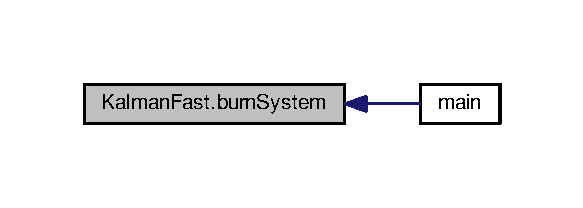
\includegraphics[width=280pt]{namespace_kalman_fast_a773a341412a385d39ed10ce68dd87bb0_icgraph}
\end{center}
\end{figure}


\hypertarget{namespace_kalman_fast_aa3688eda0919f31279971be1007f5ceb}{\index{Kalman\-Fast@{Kalman\-Fast}!burn\-System\-Fixed@{burn\-System\-Fixed}}
\index{burn\-System\-Fixed@{burn\-System\-Fixed}!KalmanFast@{Kalman\-Fast}}
\subsubsection[{burn\-System\-Fixed}]{\setlength{\rightskip}{0pt plus 5cm}def Kalman\-Fast.\-burn\-System\-Fixed (
\begin{DoxyParamCaption}
\item[{}]{X, }
\item[{}]{F, }
\item[{}]{D, }
\item[{}]{dist, }
\item[{}]{num\-Burn, }
\item[{}]{burn\-Rand}
\end{DoxyParamCaption}
)}}\label{namespace_kalman_fast_aa3688eda0919f31279971be1007f5ceb}


Definition at line 97 of file Kalman\-Fast.\-py.

\hypertarget{namespace_kalman_fast_a93baa236856614fff1114e942663c940}{\index{Kalman\-Fast@{Kalman\-Fast}!check\-Params@{check\-Params}}
\index{check\-Params@{check\-Params}!KalmanFast@{Kalman\-Fast}}
\subsubsection[{check\-Params}]{\setlength{\rightskip}{0pt plus 5cm}def Kalman\-Fast.\-check\-Params (
\begin{DoxyParamCaption}
\item[{}]{p\-List = {\ttfamily None}, }
\item[{}]{q\-List = {\ttfamily None}, }
\item[{}]{dist = {\ttfamily None}}
\end{DoxyParamCaption}
)}}\label{namespace_kalman_fast_a93baa236856614fff1114e942663c940}


Definition at line 26 of file Kalman\-Fast.\-py.

\hypertarget{namespace_kalman_fast_a4becb61d8d27132af8940ddf2717f13a}{\index{Kalman\-Fast@{Kalman\-Fast}!fixed\-Interval\-Smoother@{fixed\-Interval\-Smoother}}
\index{fixed\-Interval\-Smoother@{fixed\-Interval\-Smoother}!KalmanFast@{Kalman\-Fast}}
\subsubsection[{fixed\-Interval\-Smoother}]{\setlength{\rightskip}{0pt plus 5cm}def Kalman\-Fast.\-fixed\-Interval\-Smoother (
\begin{DoxyParamCaption}
\item[{}]{y, }
\item[{}]{r, }
\item[{}]{x, }
\item[{}]{X, }
\item[{}]{P, }
\item[{}]{X\-Minus, }
\item[{}]{P\-Minus, }
\item[{}]{F, }
\item[{}]{I, }
\item[{}]{D, }
\item[{}]{Q, }
\item[{}]{H, }
\item[{}]{R, }
\item[{}]{K}
\end{DoxyParamCaption}
)}}\label{namespace_kalman_fast_a4becb61d8d27132af8940ddf2717f13a}


Definition at line 372 of file Kalman\-Fast.\-py.

\hypertarget{namespace_kalman_fast_aff10a690431ea74c678c101767811865}{\index{Kalman\-Fast@{Kalman\-Fast}!get\-Ln\-Like@{get\-Ln\-Like}}
\index{get\-Ln\-Like@{get\-Ln\-Like}!KalmanFast@{Kalman\-Fast}}
\subsubsection[{get\-Ln\-Like}]{\setlength{\rightskip}{0pt plus 5cm}def Kalman\-Fast.\-get\-Ln\-Like (
\begin{DoxyParamCaption}
\item[{}]{y, }
\item[{}]{mask, }
\item[{}]{X, }
\item[{}]{P, }
\item[{}]{X\-Minus, }
\item[{}]{P\-Minus, }
\item[{}]{F, }
\item[{}]{I, }
\item[{}]{D, }
\item[{}]{Q, }
\item[{}]{H, }
\item[{}]{R, }
\item[{}]{K}
\end{DoxyParamCaption}
)}}\label{namespace_kalman_fast_aff10a690431ea74c678c101767811865}


Definition at line 222 of file Kalman\-Fast.\-py.

\hypertarget{namespace_kalman_fast_aa58a01d0dc5d786acd10e70f29572750}{\index{Kalman\-Fast@{Kalman\-Fast}!get\-Ln\-Like\-Missing@{get\-Ln\-Like\-Missing}}
\index{get\-Ln\-Like\-Missing@{get\-Ln\-Like\-Missing}!KalmanFast@{Kalman\-Fast}}
\subsubsection[{get\-Ln\-Like\-Missing}]{\setlength{\rightskip}{0pt plus 5cm}def Kalman\-Fast.\-get\-Ln\-Like\-Missing (
\begin{DoxyParamCaption}
\item[{}]{y, }
\item[{}]{mask, }
\item[{}]{X, }
\item[{}]{P, }
\item[{}]{X\-Minus, }
\item[{}]{P\-Minus, }
\item[{}]{F, }
\item[{}]{I, }
\item[{}]{D, }
\item[{}]{Q, }
\item[{}]{H, }
\item[{}]{R, }
\item[{}]{K}
\end{DoxyParamCaption}
)}}\label{namespace_kalman_fast_aa58a01d0dc5d786acd10e70f29572750}


Definition at line 323 of file Kalman\-Fast.\-py.

\hypertarget{namespace_kalman_fast_a9bd7e9be6130240320b671d5b4926a23}{\index{Kalman\-Fast@{Kalman\-Fast}!get\-Residuals@{get\-Residuals}}
\index{get\-Residuals@{get\-Residuals}!KalmanFast@{Kalman\-Fast}}
\subsubsection[{get\-Residuals}]{\setlength{\rightskip}{0pt plus 5cm}def Kalman\-Fast.\-get\-Residuals (
\begin{DoxyParamCaption}
\item[{}]{y, }
\item[{}]{r, }
\item[{}]{X, }
\item[{}]{P, }
\item[{}]{X\-Minus, }
\item[{}]{P\-Minus, }
\item[{}]{F, }
\item[{}]{I, }
\item[{}]{D, }
\item[{}]{Q, }
\item[{}]{H, }
\item[{}]{R, }
\item[{}]{K}
\end{DoxyParamCaption}
)}}\label{namespace_kalman_fast_a9bd7e9be6130240320b671d5b4926a23}


Definition at line 348 of file Kalman\-Fast.\-py.

\hypertarget{namespace_kalman_fast_a2e58cd85931f067069622355623d60f7}{\index{Kalman\-Fast@{Kalman\-Fast}!make\-System@{make\-System}}
\index{make\-System@{make\-System}!KalmanFast@{Kalman\-Fast}}
\subsubsection[{make\-System}]{\setlength{\rightskip}{0pt plus 5cm}def Kalman\-Fast.\-make\-System (
\begin{DoxyParamCaption}
\item[{}]{p, }
\item[{}]{q}
\end{DoxyParamCaption}
)}}\label{namespace_kalman_fast_a2e58cd85931f067069622355623d60f7}


Definition at line 10 of file Kalman\-Fast.\-py.

\hypertarget{namespace_kalman_fast_acf131e0bf3988ca746748906158dc85f}{\index{Kalman\-Fast@{Kalman\-Fast}!obs\-System@{obs\-System}}
\index{obs\-System@{obs\-System}!KalmanFast@{Kalman\-Fast}}
\subsubsection[{obs\-System}]{\setlength{\rightskip}{0pt plus 5cm}def Kalman\-Fast.\-obs\-System (
\begin{DoxyParamCaption}
\item[{}]{X, }
\item[{}]{F, }
\item[{}]{D, }
\item[{}]{H, }
\item[{}]{dist, }
\item[{}]{noise, }
\item[{}]{y, }
\item[{}]{num\-Obs, }
\item[{}]{dist\-Seed, }
\item[{}]{noise\-Seed}
\end{DoxyParamCaption}
)}}\label{namespace_kalman_fast_acf131e0bf3988ca746748906158dc85f}


Definition at line 166 of file Kalman\-Fast.\-py.

\hypertarget{namespace_kalman_fast_a2ca9007cfa54c66b77cabd70e599395e}{\index{Kalman\-Fast@{Kalman\-Fast}!obs\-System\-Fixed@{obs\-System\-Fixed}}
\index{obs\-System\-Fixed@{obs\-System\-Fixed}!KalmanFast@{Kalman\-Fast}}
\subsubsection[{obs\-System\-Fixed}]{\setlength{\rightskip}{0pt plus 5cm}def Kalman\-Fast.\-obs\-System\-Fixed (
\begin{DoxyParamCaption}
\item[{}]{X, }
\item[{}]{F, }
\item[{}]{D, }
\item[{}]{H, }
\item[{}]{dist, }
\item[{}]{noise, }
\item[{}]{y, }
\item[{}]{num\-Obs, }
\item[{}]{dist\-Rand, }
\item[{}]{noise\-Rand}
\end{DoxyParamCaption}
)}}\label{namespace_kalman_fast_a2ca9007cfa54c66b77cabd70e599395e}


Definition at line 127 of file Kalman\-Fast.\-py.

\hypertarget{namespace_kalman_fast_ab15297ce7c869d9c749f8ac170fc091e}{\index{Kalman\-Fast@{Kalman\-Fast}!obs\-System\-Fixed\-Missing@{obs\-System\-Fixed\-Missing}}
\index{obs\-System\-Fixed\-Missing@{obs\-System\-Fixed\-Missing}!KalmanFast@{Kalman\-Fast}}
\subsubsection[{obs\-System\-Fixed\-Missing}]{\setlength{\rightskip}{0pt plus 5cm}def Kalman\-Fast.\-obs\-System\-Fixed\-Missing (
\begin{DoxyParamCaption}
\item[{}]{X, }
\item[{}]{F, }
\item[{}]{D, }
\item[{}]{H, }
\item[{}]{dist, }
\item[{}]{noise, }
\item[{}]{y, }
\item[{}]{mask, }
\item[{}]{num\-Obs, }
\item[{}]{dist\-Rand, }
\item[{}]{noise\-Rand}
\end{DoxyParamCaption}
)}}\label{namespace_kalman_fast_ab15297ce7c869d9c749f8ac170fc091e}


Definition at line 145 of file Kalman\-Fast.\-py.

\hypertarget{namespace_kalman_fast_a742169bce77d3a99ff5806e4bff223ee}{\index{Kalman\-Fast@{Kalman\-Fast}!obs\-System\-Missing@{obs\-System\-Missing}}
\index{obs\-System\-Missing@{obs\-System\-Missing}!KalmanFast@{Kalman\-Fast}}
\subsubsection[{obs\-System\-Missing}]{\setlength{\rightskip}{0pt plus 5cm}def Kalman\-Fast.\-obs\-System\-Missing (
\begin{DoxyParamCaption}
\item[{}]{X, }
\item[{}]{F, }
\item[{}]{D, }
\item[{}]{H, }
\item[{}]{dist, }
\item[{}]{noise, }
\item[{}]{y, }
\item[{}]{mask, }
\item[{}]{num\-Obs, }
\item[{}]{dist\-Seed, }
\item[{}]{noise\-Seed}
\end{DoxyParamCaption}
)}}\label{namespace_kalman_fast_a742169bce77d3a99ff5806e4bff223ee}


Definition at line 192 of file Kalman\-Fast.\-py.

\hypertarget{namespace_kalman_fast_a599ed523e7fcf7ac22112248d8a31c4d}{\index{Kalman\-Fast@{Kalman\-Fast}!set\-System@{set\-System}}
\index{set\-System@{set\-System}!KalmanFast@{Kalman\-Fast}}
\subsubsection[{set\-System}]{\setlength{\rightskip}{0pt plus 5cm}def Kalman\-Fast.\-set\-System (
\begin{DoxyParamCaption}
\item[{}]{p, }
\item[{}]{q, }
\item[{}]{m, }
\item[{}]{p\-List, }
\item[{}]{q\-List, }
\item[{}]{dist, }
\item[{}]{F, }
\item[{}]{I, }
\item[{}]{D, }
\item[{}]{Q}
\end{DoxyParamCaption}
)}}\label{namespace_kalman_fast_a599ed523e7fcf7ac22112248d8a31c4d}


Definition at line 67 of file Kalman\-Fast.\-py.



Here is the call graph for this function\-:\nopagebreak
\begin{figure}[H]
\begin{center}
\leavevmode
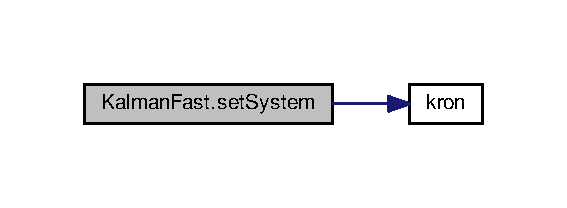
\includegraphics[width=272pt]{namespace_kalman_fast_a599ed523e7fcf7ac22112248d8a31c4d_cgraph}
\end{center}
\end{figure}


\hypertarget{namespace_kalman_fast_a308c13060d7fef2e08c668baa4f5c3fb}{\index{Kalman\-Fast@{Kalman\-Fast}!set\-System\-Diffuse@{set\-System\-Diffuse}}
\index{set\-System\-Diffuse@{set\-System\-Diffuse}!KalmanFast@{Kalman\-Fast}}
\subsubsection[{set\-System\-Diffuse}]{\setlength{\rightskip}{0pt plus 5cm}def Kalman\-Fast.\-set\-System\-Diffuse (
\begin{DoxyParamCaption}
\item[{}]{p, }
\item[{}]{q, }
\item[{}]{m, }
\item[{}]{p\-List, }
\item[{}]{q\-List, }
\item[{}]{dist, }
\item[{}]{F, }
\item[{}]{I, }
\item[{}]{D, }
\item[{}]{Q}
\end{DoxyParamCaption}
)}}\label{namespace_kalman_fast_a308c13060d7fef2e08c668baa4f5c3fb}


Definition at line 82 of file Kalman\-Fast.\-py.


\hypertarget{namespacempl__settings}{\section{mpl\-\_\-settings Namespace Reference}
\label{namespacempl__settings}\index{mpl\-\_\-settings@{mpl\-\_\-settings}}
}
\subsection*{Functions}
\begin{DoxyCompactItemize}
\item 
def \hyperlink{namespacempl__settings_a0d7883b3b39d3ab7ed7382a9688ac9e3}{set\-\_\-plot\-\_\-params}
\end{DoxyCompactItemize}


\subsection{Function Documentation}
\hypertarget{namespacempl__settings_a0d7883b3b39d3ab7ed7382a9688ac9e3}{\index{mpl\-\_\-settings@{mpl\-\_\-settings}!set\-\_\-plot\-\_\-params@{set\-\_\-plot\-\_\-params}}
\index{set\-\_\-plot\-\_\-params@{set\-\_\-plot\-\_\-params}!mpl_settings@{mpl\-\_\-settings}}
\subsubsection[{set\-\_\-plot\-\_\-params}]{\setlength{\rightskip}{0pt plus 5cm}def mpl\-\_\-settings.\-set\-\_\-plot\-\_\-params (
\begin{DoxyParamCaption}
\item[{}]{fontsize = {\ttfamily 20}}
\end{DoxyParamCaption}
)}}\label{namespacempl__settings_a0d7883b3b39d3ab7ed7382a9688ac9e3}


Definition at line 3 of file mpl\-\_\-settings.\-py.



Here is the caller graph for this function\-:\nopagebreak
\begin{figure}[H]
\begin{center}
\leavevmode
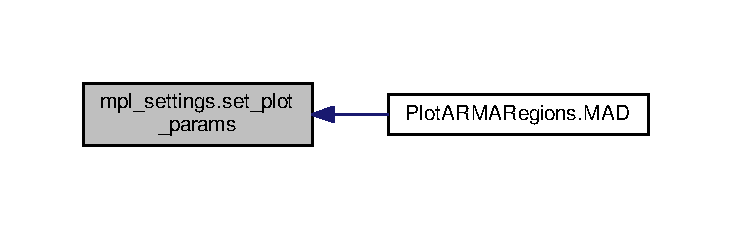
\includegraphics[width=350pt]{namespacempl__settings_a0d7883b3b39d3ab7ed7382a9688ac9e3_icgraph}
\end{center}
\end{figure}



\hypertarget{namespace_plot_a_r_m_a_regions}{\section{Plot\-A\-R\-M\-A\-Regions Namespace Reference}
\label{namespace_plot_a_r_m_a_regions}\index{Plot\-A\-R\-M\-A\-Regions@{Plot\-A\-R\-M\-A\-Regions}}
}
\subsection*{Functions}
\begin{DoxyCompactItemize}
\item 
def \hyperlink{namespace_plot_a_r_m_a_regions_ab8d32e5943f6391d1de1d360f78a4e1c}{M\-A\-D}
\end{DoxyCompactItemize}
\subsection*{Variables}
\begin{DoxyCompactItemize}
\item 
float \hyperlink{namespace_plot_a_r_m_a_regions_a911f440b0b304e72e7588c7508cacd20}{sec\-Per\-Sidereal\-Day} = 86164.\-0905
\item 
float \hyperlink{namespace_plot_a_r_m_a_regions_a54e4c79468e19409c96e67dfdb482f0a}{int\-Time} = 6.\-019802903
\item 
float \hyperlink{namespace_plot_a_r_m_a_regions_a5329612770d2afb1002bfc0672f392d8}{read\-Time} = 0.\-5189485261
\item 
int \hyperlink{namespace_plot_a_r_m_a_regions_a9a622e1006cc8cc55b062f42b9e4c980}{num\-Int\-L\-C} = 270
\item 
tuple \hyperlink{namespace_plot_a_r_m_a_regions_a7b437af6d1c5ce7f40b5f27233d5f4b1}{deltat} = (\hyperlink{namespace_plot_a_r_m_a_regions_a9a622e1006cc8cc55b062f42b9e4c980}{num\-Int\-L\-C}$\ast$(\hyperlink{namespace_plot_a_r_m_a_regions_a54e4c79468e19409c96e67dfdb482f0a}{int\-Time}+\hyperlink{namespace_plot_a_r_m_a_regions_a5329612770d2afb1002bfc0672f392d8}{read\-Time}))
\item 
string \hyperlink{namespace_plot_a_r_m_a_regions_a35b8724b6b0849cfed30c080d79c775e}{Tri\-File\-Path} = base\-Path+'mcmc\-Out\-\_\-\%d\-\_\-\%d.\-dat'
\item 
tuple \hyperlink{namespace_plot_a_r_m_a_regions_a418058aa77527961189e1d40f3d8091d}{Tri\-File} = open(\hyperlink{namespace_plot_a_r_m_a_regions_a35b8724b6b0849cfed30c080d79c775e}{Tri\-File\-Path})
\item 
tuple \hyperlink{namespace_plot_a_r_m_a_regions_a478b5b50b6eddf2098c4a31f8a83b86d}{line} = Tri\-File.\-readline()
\item 
tuple \hyperlink{namespace_plot_a_r_m_a_regions_a4e1eb2c62fce8e30d2ac6b5152291a8a}{values} = line.\-split()
\item 
tuple \hyperlink{namespace_plot_a_r_m_a_regions_a400da7acac41459d918d50e10fcd9735}{nsteps} = int(\hyperlink{namespace_plot_a_r_m_a_regions_a4e1eb2c62fce8e30d2ac6b5152291a8a}{values}\mbox{[}1\mbox{]})
\item 
tuple \hyperlink{namespace_plot_a_r_m_a_regions_ad8d2b4da6dbf7506bdf2e3ae4a66e626}{nwalkers} = int(\hyperlink{namespace_plot_a_r_m_a_regions_a4e1eb2c62fce8e30d2ac6b5152291a8a}{values}\mbox{[}1\mbox{]})
\item 
tuple \hyperlink{namespace_plot_a_r_m_a_regions_a6d9523e891d3f88e36e2c83da27f05a9}{ndim} = int(\hyperlink{namespace_plot_a_r_m_a_regions_a4e1eb2c62fce8e30d2ac6b5152291a8a}{values}\mbox{[}1\mbox{]})
\item 
tuple \hyperlink{namespace_plot_a_r_m_a_regions_a3c04a644963d85e8e23169a93ce616be}{walkers} = np.\-zeros((\hyperlink{namespace_plot_a_r_m_a_regions_a400da7acac41459d918d50e10fcd9735}{nsteps},\hyperlink{namespace_plot_a_r_m_a_regions_ad8d2b4da6dbf7506bdf2e3ae4a66e626}{nwalkers},\hyperlink{namespace_plot_a_r_m_a_regions_a6d9523e891d3f88e36e2c83da27f05a9}{ndim}))
\item 
tuple \hyperlink{namespace_plot_a_r_m_a_regions_a52850befe6ca5dd531f3da54183de7af}{median\-Walker} = np.\-zeros((\hyperlink{namespace_plot_a_r_m_a_regions_a400da7acac41459d918d50e10fcd9735}{nsteps},\hyperlink{namespace_plot_a_r_m_a_regions_a6d9523e891d3f88e36e2c83da27f05a9}{ndim}))
\item 
tuple \hyperlink{namespace_plot_a_r_m_a_regions_aebce0372a3a0163d83eb67756a668e9c}{median\-Dev\-Walker} = np.\-zeros((\hyperlink{namespace_plot_a_r_m_a_regions_a400da7acac41459d918d50e10fcd9735}{nsteps},\hyperlink{namespace_plot_a_r_m_a_regions_a6d9523e891d3f88e36e2c83da27f05a9}{ndim}))
\item 
tuple \hyperlink{namespace_plot_a_r_m_a_regions_aeab291d1791e6713eb80e5d400f942f5}{step\-Arr} = np.\-arange(\hyperlink{namespace_plot_a_r_m_a_regions_a400da7acac41459d918d50e10fcd9735}{nsteps})
\item 
list \hyperlink{namespace_plot_a_r_m_a_regions_aa67f172c43ed86ba8625f428144531b0}{samples} = \hyperlink{namespace_plot_a_r_m_a_regions_a3c04a644963d85e8e23169a93ce616be}{walkers}\mbox{[}chop\-:,\-:,\-:\mbox{]}
\item 
tuple \hyperlink{namespace_plot_a_r_m_a_regions_aeadeb0d1d3349eeeafd2ee3cf0c17c41}{lbls} = list()
\end{DoxyCompactItemize}


\subsection{Function Documentation}
\hypertarget{namespace_plot_a_r_m_a_regions_ab8d32e5943f6391d1de1d360f78a4e1c}{\index{Plot\-A\-R\-M\-A\-Regions@{Plot\-A\-R\-M\-A\-Regions}!M\-A\-D@{M\-A\-D}}
\index{M\-A\-D@{M\-A\-D}!PlotARMARegions@{Plot\-A\-R\-M\-A\-Regions}}
\subsubsection[{M\-A\-D}]{\setlength{\rightskip}{0pt plus 5cm}def Plot\-A\-R\-M\-A\-Regions.\-M\-A\-D (
\begin{DoxyParamCaption}
\item[{}]{a}
\end{DoxyParamCaption}
)}}\label{namespace_plot_a_r_m_a_regions_ab8d32e5943f6391d1de1d360f78a4e1c}


Definition at line 18 of file Plot\-A\-R\-M\-A\-Regions.\-py.



Here is the call graph for this function\-:\nopagebreak
\begin{figure}[H]
\begin{center}
\leavevmode
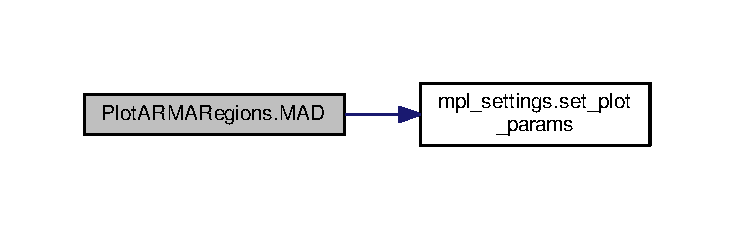
\includegraphics[width=350pt]{namespace_plot_a_r_m_a_regions_ab8d32e5943f6391d1de1d360f78a4e1c_cgraph}
\end{center}
\end{figure}




\subsection{Variable Documentation}
\hypertarget{namespace_plot_a_r_m_a_regions_a7b437af6d1c5ce7f40b5f27233d5f4b1}{\index{Plot\-A\-R\-M\-A\-Regions@{Plot\-A\-R\-M\-A\-Regions}!deltat@{deltat}}
\index{deltat@{deltat}!PlotARMARegions@{Plot\-A\-R\-M\-A\-Regions}}
\subsubsection[{deltat}]{\setlength{\rightskip}{0pt plus 5cm}tuple Plot\-A\-R\-M\-A\-Regions.\-deltat = ({\bf num\-Int\-L\-C}$\ast$({\bf int\-Time}+{\bf read\-Time}))}}\label{namespace_plot_a_r_m_a_regions_a7b437af6d1c5ce7f40b5f27233d5f4b1}


Definition at line 16 of file Plot\-A\-R\-M\-A\-Regions.\-py.

\hypertarget{namespace_plot_a_r_m_a_regions_a54e4c79468e19409c96e67dfdb482f0a}{\index{Plot\-A\-R\-M\-A\-Regions@{Plot\-A\-R\-M\-A\-Regions}!int\-Time@{int\-Time}}
\index{int\-Time@{int\-Time}!PlotARMARegions@{Plot\-A\-R\-M\-A\-Regions}}
\subsubsection[{int\-Time}]{\setlength{\rightskip}{0pt plus 5cm}float Plot\-A\-R\-M\-A\-Regions.\-int\-Time = 6.\-019802903}}\label{namespace_plot_a_r_m_a_regions_a54e4c79468e19409c96e67dfdb482f0a}


Definition at line 13 of file Plot\-A\-R\-M\-A\-Regions.\-py.

\hypertarget{namespace_plot_a_r_m_a_regions_aeadeb0d1d3349eeeafd2ee3cf0c17c41}{\index{Plot\-A\-R\-M\-A\-Regions@{Plot\-A\-R\-M\-A\-Regions}!lbls@{lbls}}
\index{lbls@{lbls}!PlotARMARegions@{Plot\-A\-R\-M\-A\-Regions}}
\subsubsection[{lbls}]{\setlength{\rightskip}{0pt plus 5cm}tuple Plot\-A\-R\-M\-A\-Regions.\-lbls = list()}}\label{namespace_plot_a_r_m_a_regions_aeadeb0d1d3349eeeafd2ee3cf0c17c41}


Definition at line 94 of file Plot\-A\-R\-M\-A\-Regions.\-py.

\hypertarget{namespace_plot_a_r_m_a_regions_a478b5b50b6eddf2098c4a31f8a83b86d}{\index{Plot\-A\-R\-M\-A\-Regions@{Plot\-A\-R\-M\-A\-Regions}!line@{line}}
\index{line@{line}!PlotARMARegions@{Plot\-A\-R\-M\-A\-Regions}}
\subsubsection[{line}]{\setlength{\rightskip}{0pt plus 5cm}tuple Plot\-A\-R\-M\-A\-Regions.\-line = Tri\-File.\-readline()}}\label{namespace_plot_a_r_m_a_regions_a478b5b50b6eddf2098c4a31f8a83b86d}


Definition at line 46 of file Plot\-A\-R\-M\-A\-Regions.\-py.

\hypertarget{namespace_plot_a_r_m_a_regions_aebce0372a3a0163d83eb67756a668e9c}{\index{Plot\-A\-R\-M\-A\-Regions@{Plot\-A\-R\-M\-A\-Regions}!median\-Dev\-Walker@{median\-Dev\-Walker}}
\index{median\-Dev\-Walker@{median\-Dev\-Walker}!PlotARMARegions@{Plot\-A\-R\-M\-A\-Regions}}
\subsubsection[{median\-Dev\-Walker}]{\setlength{\rightskip}{0pt plus 5cm}tuple Plot\-A\-R\-M\-A\-Regions.\-median\-Dev\-Walker = np.\-zeros(({\bf nsteps},{\bf ndim}))}}\label{namespace_plot_a_r_m_a_regions_aebce0372a3a0163d83eb67756a668e9c}


Definition at line 69 of file Plot\-A\-R\-M\-A\-Regions.\-py.

\hypertarget{namespace_plot_a_r_m_a_regions_a52850befe6ca5dd531f3da54183de7af}{\index{Plot\-A\-R\-M\-A\-Regions@{Plot\-A\-R\-M\-A\-Regions}!median\-Walker@{median\-Walker}}
\index{median\-Walker@{median\-Walker}!PlotARMARegions@{Plot\-A\-R\-M\-A\-Regions}}
\subsubsection[{median\-Walker}]{\setlength{\rightskip}{0pt plus 5cm}tuple Plot\-A\-R\-M\-A\-Regions.\-median\-Walker = np.\-zeros(({\bf nsteps},{\bf ndim}))}}\label{namespace_plot_a_r_m_a_regions_a52850befe6ca5dd531f3da54183de7af}


Definition at line 68 of file Plot\-A\-R\-M\-A\-Regions.\-py.

\hypertarget{namespace_plot_a_r_m_a_regions_a6d9523e891d3f88e36e2c83da27f05a9}{\index{Plot\-A\-R\-M\-A\-Regions@{Plot\-A\-R\-M\-A\-Regions}!ndim@{ndim}}
\index{ndim@{ndim}!PlotARMARegions@{Plot\-A\-R\-M\-A\-Regions}}
\subsubsection[{ndim}]{\setlength{\rightskip}{0pt plus 5cm}tuple Plot\-A\-R\-M\-A\-Regions.\-ndim = int({\bf values}\mbox{[}1\mbox{]})}}\label{namespace_plot_a_r_m_a_regions_a6d9523e891d3f88e36e2c83da27f05a9}


Definition at line 57 of file Plot\-A\-R\-M\-A\-Regions.\-py.

\hypertarget{namespace_plot_a_r_m_a_regions_a400da7acac41459d918d50e10fcd9735}{\index{Plot\-A\-R\-M\-A\-Regions@{Plot\-A\-R\-M\-A\-Regions}!nsteps@{nsteps}}
\index{nsteps@{nsteps}!PlotARMARegions@{Plot\-A\-R\-M\-A\-Regions}}
\subsubsection[{nsteps}]{\setlength{\rightskip}{0pt plus 5cm}tuple Plot\-A\-R\-M\-A\-Regions.\-nsteps = int({\bf values}\mbox{[}1\mbox{]})}}\label{namespace_plot_a_r_m_a_regions_a400da7acac41459d918d50e10fcd9735}


Definition at line 49 of file Plot\-A\-R\-M\-A\-Regions.\-py.

\hypertarget{namespace_plot_a_r_m_a_regions_a9a622e1006cc8cc55b062f42b9e4c980}{\index{Plot\-A\-R\-M\-A\-Regions@{Plot\-A\-R\-M\-A\-Regions}!num\-Int\-L\-C@{num\-Int\-L\-C}}
\index{num\-Int\-L\-C@{num\-Int\-L\-C}!PlotARMARegions@{Plot\-A\-R\-M\-A\-Regions}}
\subsubsection[{num\-Int\-L\-C}]{\setlength{\rightskip}{0pt plus 5cm}int Plot\-A\-R\-M\-A\-Regions.\-num\-Int\-L\-C = 270}}\label{namespace_plot_a_r_m_a_regions_a9a622e1006cc8cc55b062f42b9e4c980}


Definition at line 15 of file Plot\-A\-R\-M\-A\-Regions.\-py.

\hypertarget{namespace_plot_a_r_m_a_regions_ad8d2b4da6dbf7506bdf2e3ae4a66e626}{\index{Plot\-A\-R\-M\-A\-Regions@{Plot\-A\-R\-M\-A\-Regions}!nwalkers@{nwalkers}}
\index{nwalkers@{nwalkers}!PlotARMARegions@{Plot\-A\-R\-M\-A\-Regions}}
\subsubsection[{nwalkers}]{\setlength{\rightskip}{0pt plus 5cm}tuple Plot\-A\-R\-M\-A\-Regions.\-nwalkers = int({\bf values}\mbox{[}1\mbox{]})}}\label{namespace_plot_a_r_m_a_regions_ad8d2b4da6dbf7506bdf2e3ae4a66e626}


Definition at line 53 of file Plot\-A\-R\-M\-A\-Regions.\-py.

\hypertarget{namespace_plot_a_r_m_a_regions_a5329612770d2afb1002bfc0672f392d8}{\index{Plot\-A\-R\-M\-A\-Regions@{Plot\-A\-R\-M\-A\-Regions}!read\-Time@{read\-Time}}
\index{read\-Time@{read\-Time}!PlotARMARegions@{Plot\-A\-R\-M\-A\-Regions}}
\subsubsection[{read\-Time}]{\setlength{\rightskip}{0pt plus 5cm}float Plot\-A\-R\-M\-A\-Regions.\-read\-Time = 0.\-5189485261}}\label{namespace_plot_a_r_m_a_regions_a5329612770d2afb1002bfc0672f392d8}


Definition at line 14 of file Plot\-A\-R\-M\-A\-Regions.\-py.

\hypertarget{namespace_plot_a_r_m_a_regions_aa67f172c43ed86ba8625f428144531b0}{\index{Plot\-A\-R\-M\-A\-Regions@{Plot\-A\-R\-M\-A\-Regions}!samples@{samples}}
\index{samples@{samples}!PlotARMARegions@{Plot\-A\-R\-M\-A\-Regions}}
\subsubsection[{samples}]{\setlength{\rightskip}{0pt plus 5cm}list Plot\-A\-R\-M\-A\-Regions.\-samples = {\bf walkers}\mbox{[}chop\-:,\-:,\-:\mbox{]}}}\label{namespace_plot_a_r_m_a_regions_aa67f172c43ed86ba8625f428144531b0}


Definition at line 93 of file Plot\-A\-R\-M\-A\-Regions.\-py.

\hypertarget{namespace_plot_a_r_m_a_regions_a911f440b0b304e72e7588c7508cacd20}{\index{Plot\-A\-R\-M\-A\-Regions@{Plot\-A\-R\-M\-A\-Regions}!sec\-Per\-Sidereal\-Day@{sec\-Per\-Sidereal\-Day}}
\index{sec\-Per\-Sidereal\-Day@{sec\-Per\-Sidereal\-Day}!PlotARMARegions@{Plot\-A\-R\-M\-A\-Regions}}
\subsubsection[{sec\-Per\-Sidereal\-Day}]{\setlength{\rightskip}{0pt plus 5cm}float Plot\-A\-R\-M\-A\-Regions.\-sec\-Per\-Sidereal\-Day = 86164.\-0905}}\label{namespace_plot_a_r_m_a_regions_a911f440b0b304e72e7588c7508cacd20}


Definition at line 12 of file Plot\-A\-R\-M\-A\-Regions.\-py.

\hypertarget{namespace_plot_a_r_m_a_regions_aeab291d1791e6713eb80e5d400f942f5}{\index{Plot\-A\-R\-M\-A\-Regions@{Plot\-A\-R\-M\-A\-Regions}!step\-Arr@{step\-Arr}}
\index{step\-Arr@{step\-Arr}!PlotARMARegions@{Plot\-A\-R\-M\-A\-Regions}}
\subsubsection[{step\-Arr}]{\setlength{\rightskip}{0pt plus 5cm}tuple Plot\-A\-R\-M\-A\-Regions.\-step\-Arr = np.\-arange({\bf nsteps})}}\label{namespace_plot_a_r_m_a_regions_aeab291d1791e6713eb80e5d400f942f5}


Definition at line 74 of file Plot\-A\-R\-M\-A\-Regions.\-py.

\hypertarget{namespace_plot_a_r_m_a_regions_a418058aa77527961189e1d40f3d8091d}{\index{Plot\-A\-R\-M\-A\-Regions@{Plot\-A\-R\-M\-A\-Regions}!Tri\-File@{Tri\-File}}
\index{Tri\-File@{Tri\-File}!PlotARMARegions@{Plot\-A\-R\-M\-A\-Regions}}
\subsubsection[{Tri\-File}]{\setlength{\rightskip}{0pt plus 5cm}tuple Plot\-A\-R\-M\-A\-Regions.\-Tri\-File = open({\bf Tri\-File\-Path})}}\label{namespace_plot_a_r_m_a_regions_a418058aa77527961189e1d40f3d8091d}


Definition at line 45 of file Plot\-A\-R\-M\-A\-Regions.\-py.

\hypertarget{namespace_plot_a_r_m_a_regions_a35b8724b6b0849cfed30c080d79c775e}{\index{Plot\-A\-R\-M\-A\-Regions@{Plot\-A\-R\-M\-A\-Regions}!Tri\-File\-Path@{Tri\-File\-Path}}
\index{Tri\-File\-Path@{Tri\-File\-Path}!PlotARMARegions@{Plot\-A\-R\-M\-A\-Regions}}
\subsubsection[{Tri\-File\-Path}]{\setlength{\rightskip}{0pt plus 5cm}string Plot\-A\-R\-M\-A\-Regions.\-Tri\-File\-Path = base\-Path+'mcmc\-Out\-\_\-\%d\-\_\-\%d.\-dat'}}\label{namespace_plot_a_r_m_a_regions_a35b8724b6b0849cfed30c080d79c775e}


Definition at line 44 of file Plot\-A\-R\-M\-A\-Regions.\-py.

\hypertarget{namespace_plot_a_r_m_a_regions_a4e1eb2c62fce8e30d2ac6b5152291a8a}{\index{Plot\-A\-R\-M\-A\-Regions@{Plot\-A\-R\-M\-A\-Regions}!values@{values}}
\index{values@{values}!PlotARMARegions@{Plot\-A\-R\-M\-A\-Regions}}
\subsubsection[{values}]{\setlength{\rightskip}{0pt plus 5cm}tuple Plot\-A\-R\-M\-A\-Regions.\-values = line.\-split()}}\label{namespace_plot_a_r_m_a_regions_a4e1eb2c62fce8e30d2ac6b5152291a8a}


Definition at line 48 of file Plot\-A\-R\-M\-A\-Regions.\-py.

\hypertarget{namespace_plot_a_r_m_a_regions_a3c04a644963d85e8e23169a93ce616be}{\index{Plot\-A\-R\-M\-A\-Regions@{Plot\-A\-R\-M\-A\-Regions}!walkers@{walkers}}
\index{walkers@{walkers}!PlotARMARegions@{Plot\-A\-R\-M\-A\-Regions}}
\subsubsection[{walkers}]{\setlength{\rightskip}{0pt plus 5cm}tuple Plot\-A\-R\-M\-A\-Regions.\-walkers = np.\-zeros(({\bf nsteps},{\bf nwalkers},{\bf ndim}))}}\label{namespace_plot_a_r_m_a_regions_a3c04a644963d85e8e23169a93ce616be}


Definition at line 58 of file Plot\-A\-R\-M\-A\-Regions.\-py.


\chapter{Class Documentation}
\hypertarget{class_c_a_r_m_a}{\section{C\-A\-R\-M\-A Class Reference}
\label{class_c_a_r_m_a}\index{C\-A\-R\-M\-A@{C\-A\-R\-M\-A}}
}


{\ttfamily \#include $<$C\-A\-R\-M\-A.\-hpp$>$}

\subsection*{Public Member Functions}
\begin{DoxyCompactItemize}
\item 
\hyperlink{class_c_a_r_m_a_a8871e02b301b503a987c03afc15c573c}{C\-A\-R\-M\-A} ()
\item 
\hyperlink{class_c_a_r_m_a_a19f2c3c41d81428c5f77a71f983dcc0b}{$\sim$\-C\-A\-R\-M\-A} ()
\item 
int \hyperlink{class_c_a_r_m_a_af758356c8aec7ea57d4edbd4c430c780}{get\-\_\-p} ()
\item 
int \hyperlink{class_c_a_r_m_a_aca44011b5238545f728d61d1cbbb72c2}{get\-\_\-q} ()
\item 
double \hyperlink{class_c_a_r_m_a_a56124e5b6da7bf480ab87edaf2b8520f}{get\-\_\-dt} ()
\item 
void \hyperlink{class_c_a_r_m_a_a08c525da441f05c0779182f32198acf6}{set\-\_\-dt} (double t\-\_\-incr)
\item 
int \hyperlink{class_c_a_r_m_a_a1ffb8686c5b54d9d4c76b2fd50a27a39}{get\-\_\-allocated} ()
\item 
void \hyperlink{class_c_a_r_m_a_a6df47e4eb5549a3108f7ec6a5e7821c2}{print\-X} ()
\item 
const double $\ast$ \hyperlink{class_c_a_r_m_a_ac1e451e382a60ab856edf63e70752074}{get\-X} () const 
\item 
void \hyperlink{class_c_a_r_m_a_a0281829307d89b518920f2a0be1c5686}{print\-P} ()
\item 
const double $\ast$ \hyperlink{class_c_a_r_m_a_a36df8bd666ea1b1ed984d5c34588e94b}{get\-P} () const 
\item 
void \hyperlink{class_c_a_r_m_a_aeecd124f696410809e879436b70af1ec}{print\-A} ()
\item 
const complex$<$ double $>$ $\ast$ \hyperlink{class_c_a_r_m_a_a1edafdc4cd83a2f7797daa212febc957}{get\-A} () const 
\item 
void \hyperlink{class_c_a_r_m_a_aec5cf02ae8c2b4d406e82c663fb69c42}{printvr} ()
\item 
const complex$<$ double $>$ $\ast$ \hyperlink{class_c_a_r_m_a_a0942ceb94c7a11df3705ad7a65b526dd}{getvr} () const 
\item 
void \hyperlink{class_c_a_r_m_a_a3145a01eae617e76e11305ca2ec4b61d}{printvr\-Inv} ()
\item 
const complex$<$ double $>$ $\ast$ \hyperlink{class_c_a_r_m_a_a05cbbdbd1978540b35f980627054caa2}{getvr\-Inv} () const 
\item 
void \hyperlink{class_c_a_r_m_a_a52ad7813fcd1aa86359bf8946fca45b4}{printw} ()
\item 
const complex$<$ double $>$ $\ast$ \hyperlink{class_c_a_r_m_a_a3e915e480eeadc65a666523b8d26064d}{getw} () const 
\item 
void \hyperlink{class_c_a_r_m_a_a8cb9254e44aa635c08059ec14a4e2248}{printexpw} ()
\item 
const complex$<$ double $>$ $\ast$ \hyperlink{class_c_a_r_m_a_a131e3f743bab72db06162b85e51bc1cf}{getexpw} () const 
\item 
void \hyperlink{class_c_a_r_m_a_ace5f4355098caa632c9aba28b2882b08}{print\-B} ()
\item 
const complex$<$ double $>$ $\ast$ \hyperlink{class_c_a_r_m_a_a0c1d34a9f872b31fdebc1fd2481ca3d1}{get\-B} () const 
\item 
void \hyperlink{class_c_a_r_m_a_a3ffc6377d85bdb5f3a4192ad5826a9df}{print\-C} ()
\item 
const complex$<$ double $>$ $\ast$ \hyperlink{class_c_a_r_m_a_af2537a7b40e800fb063943b9c469cee9}{get\-C} () const 
\item 
void \hyperlink{class_c_a_r_m_a_a003b1ea5dac58b64dba766b06991103a}{print\-F} ()
\item 
const double $\ast$ \hyperlink{class_c_a_r_m_a_a74e6e4db5aa53ee0c88d93cc92e08e6d}{get\-F} () const 
\item 
void \hyperlink{class_c_a_r_m_a_a484c74e9fbbdb718b449fd07d192ef9c}{print\-Sigma} ()
\item 
const double $\ast$ \hyperlink{class_c_a_r_m_a_ae8966239bdea7a3fc242837463d23321}{get\-Sigma} () const 
\item 
void \hyperlink{class_c_a_r_m_a_ac9b01a1959b935de28e65904529b190b}{print\-Q} ()
\item 
const double $\ast$ \hyperlink{class_c_a_r_m_a_a5ee2f32bd6e67fc81ec1088ae305dfb8}{get\-Q} () const 
\item 
void \hyperlink{class_c_a_r_m_a_a3e426d288da8c4a69995be2edb72bf8d}{print\-T} ()
\item 
const double $\ast$ \hyperlink{class_c_a_r_m_a_a2f6879444895bae5b42791d13ec9b4a1}{get\-T} () const 
\item 
void \hyperlink{class_c_a_r_m_a_a6f96e596ba4a66b3f9eb7234292ad1d0}{alloc\-C\-A\-R\-M\-A} (int num\-P, int num\-Q)
\item 
void \hyperlink{class_c_a_r_m_a_af850b7e2ba5af3ae028aacfc0891b830}{dealloc\-C\-A\-R\-M\-A} ()
\item 
int \hyperlink{class_c_a_r_m_a_a20702c73019e9eafae573df3df0128d3}{check\-C\-A\-R\-M\-A\-Params} (double $\ast$Theta\-In)
\item 
void \hyperlink{class_c_a_r_m_a_a6c1c104dcf44e34fb596c6068239347e}{set\-C\-A\-R\-M\-A} (double $\ast$Theta\-In)
\item 
void \hyperlink{class_c_a_r_m_a_ad4391fa9d2ae5f6673b9ac762fd1795a}{solve\-C\-A\-R\-M\-A} ()
\item 
void \hyperlink{class_c_a_r_m_a_a8748732c23bc65486b9df8f25a905cf9}{reset\-State} (double Init\-Uncertainty)
\item 
void \hyperlink{class_c_a_r_m_a_a44b60949dc1cbcccb24873a117faa5ac}{reset\-State} ()
\item 
void \hyperlink{class_c_a_r_m_a_a98f282f6809e1e2c19ed10b362048fdc}{get\-C\-A\-R\-Roots} (complex$<$ double $>$ $\ast$\&C\-A\-Roots)
\item 
void \hyperlink{class_c_a_r_m_a_aead4fd2cb0a4f1670e866435a09e0d50}{get\-C\-M\-A\-Roots} (complex$<$ double $>$ $\ast$\&C\-M\-A\-Roots)
\item 
double \hyperlink{class_c_a_r_m_a_a2950241c0e1f1157e5b2d07e497e9b14}{get\-Intrinsic\-Var} ()
\item 
void \hyperlink{class_c_a_r_m_a_a684661827088a58ccc3131184e7506ba}{burn\-System} (int num\-Burn, unsigned int burn\-Seed, double $\ast$burn\-Rand)
\item 
void \hyperlink{class_c_a_r_m_a_a9c4a1c1471281a20e9dabc3b8a7ae527}{observe\-System} (\hyperlink{struct_ln_like_data}{Ln\-Like\-Data} $\ast$ptr2\-Ln\-Like\-Data, unsigned int dist\-Seed, double $\ast$dist\-Rand)
\item 
double \hyperlink{class_c_a_r_m_a_a44e19a15aba1f78becebc2d01a6a3a97}{get\-Mean\-Flux} (\hyperlink{struct_ln_like_data}{Ln\-Like\-Data} $\ast$ptr2\-Data)
\item 
void \hyperlink{class_c_a_r_m_a_a8dab0a97d457c89d11727fcc664fd3f3}{add\-Noise} (\hyperlink{struct_ln_like_data}{Ln\-Like\-Data} $\ast$ptr2\-Ln\-Like\-Data, unsigned int noise\-Seed, double $\ast$noise\-Rand)
\item 
double \hyperlink{class_c_a_r_m_a_af8f65514684e13060bf6614d2401c3dd}{compute\-Ln\-Likelihood} (\hyperlink{struct_ln_like_data}{Ln\-Like\-Data} $\ast$ptr2\-Ln\-Like\-Data)
\item 
double \hyperlink{class_c_a_r_m_a_aec6ca9d09edc9a5a4a69c4ccec69a6a3}{compute\-Ln\-Prior} (\hyperlink{struct_ln_like_data}{Ln\-Like\-Data} $\ast$ptr2\-Ln\-Like\-Data)
\end{DoxyCompactItemize}


\subsection{Detailed Description}


Definition at line 38 of file C\-A\-R\-M\-A.\-hpp.



\subsection{Constructor \& Destructor Documentation}
\hypertarget{class_c_a_r_m_a_a8871e02b301b503a987c03afc15c573c}{\index{C\-A\-R\-M\-A@{C\-A\-R\-M\-A}!C\-A\-R\-M\-A@{C\-A\-R\-M\-A}}
\index{C\-A\-R\-M\-A@{C\-A\-R\-M\-A}!CARMA@{C\-A\-R\-M\-A}}
\subsubsection[{C\-A\-R\-M\-A}]{\setlength{\rightskip}{0pt plus 5cm}C\-A\-R\-M\-A\-::\-C\-A\-R\-M\-A (
\begin{DoxyParamCaption}
{}
\end{DoxyParamCaption}
)}}\label{class_c_a_r_m_a_a8871e02b301b503a987c03afc15c573c}
Object that holds data and methods for performing C-\/\-A\-R\-M\-A analysis. D\-L\-M objects hold pointers to blocks of data that are set as required based on the size of the C-\/\-A\-R\-M\-A model. 

Definition at line 414 of file C\-A\-R\-M\-A.\-cpp.

\hypertarget{class_c_a_r_m_a_a19f2c3c41d81428c5f77a71f983dcc0b}{\index{C\-A\-R\-M\-A@{C\-A\-R\-M\-A}!$\sim$\-C\-A\-R\-M\-A@{$\sim$\-C\-A\-R\-M\-A}}
\index{$\sim$\-C\-A\-R\-M\-A@{$\sim$\-C\-A\-R\-M\-A}!CARMA@{C\-A\-R\-M\-A}}
\subsubsection[{$\sim$\-C\-A\-R\-M\-A}]{\setlength{\rightskip}{0pt plus 5cm}C\-A\-R\-M\-A\-::$\sim$\-C\-A\-R\-M\-A (
\begin{DoxyParamCaption}
{}
\end{DoxyParamCaption}
)}}\label{class_c_a_r_m_a_a19f2c3c41d81428c5f77a71f983dcc0b}


Definition at line 479 of file C\-A\-R\-M\-A.\-cpp.



\subsection{Member Function Documentation}
\hypertarget{class_c_a_r_m_a_a8dab0a97d457c89d11727fcc664fd3f3}{\index{C\-A\-R\-M\-A@{C\-A\-R\-M\-A}!add\-Noise@{add\-Noise}}
\index{add\-Noise@{add\-Noise}!CARMA@{C\-A\-R\-M\-A}}
\subsubsection[{add\-Noise}]{\setlength{\rightskip}{0pt plus 5cm}void C\-A\-R\-M\-A\-::add\-Noise (
\begin{DoxyParamCaption}
\item[{{\bf Ln\-Like\-Data} $\ast$}]{ptr2\-Ln\-Like\-Data, }
\item[{unsigned int}]{noise\-Seed, }
\item[{double $\ast$}]{noise\-Rand}
\end{DoxyParamCaption}
)}}\label{class_c_a_r_m_a_a8dab0a97d457c89d11727fcc664fd3f3}


Definition at line 1997 of file C\-A\-R\-M\-A.\-cpp.

\hypertarget{class_c_a_r_m_a_a6f96e596ba4a66b3f9eb7234292ad1d0}{\index{C\-A\-R\-M\-A@{C\-A\-R\-M\-A}!alloc\-C\-A\-R\-M\-A@{alloc\-C\-A\-R\-M\-A}}
\index{alloc\-C\-A\-R\-M\-A@{alloc\-C\-A\-R\-M\-A}!CARMA@{C\-A\-R\-M\-A}}
\subsubsection[{alloc\-C\-A\-R\-M\-A}]{\setlength{\rightskip}{0pt plus 5cm}void C\-A\-R\-M\-A\-::alloc\-C\-A\-R\-M\-A (
\begin{DoxyParamCaption}
\item[{int}]{num\-P, }
\item[{int}]{num\-Q}
\end{DoxyParamCaption}
)}}\label{class_c_a_r_m_a_a6f96e596ba4a66b3f9eb7234292ad1d0}


Definition at line 542 of file C\-A\-R\-M\-A.\-cpp.



Here is the caller graph for this function\-:


\hypertarget{class_c_a_r_m_a_a684661827088a58ccc3131184e7506ba}{\index{C\-A\-R\-M\-A@{C\-A\-R\-M\-A}!burn\-System@{burn\-System}}
\index{burn\-System@{burn\-System}!CARMA@{C\-A\-R\-M\-A}}
\subsubsection[{burn\-System}]{\setlength{\rightskip}{0pt plus 5cm}void C\-A\-R\-M\-A\-::burn\-System (
\begin{DoxyParamCaption}
\item[{int}]{num\-Burn, }
\item[{unsigned int}]{burn\-Seed, }
\item[{double $\ast$}]{burn\-Rand}
\end{DoxyParamCaption}
)}}\label{class_c_a_r_m_a_a684661827088a58ccc3131184e7506ba}


Definition at line 1893 of file C\-A\-R\-M\-A.\-cpp.

\hypertarget{class_c_a_r_m_a_a20702c73019e9eafae573df3df0128d3}{\index{C\-A\-R\-M\-A@{C\-A\-R\-M\-A}!check\-C\-A\-R\-M\-A\-Params@{check\-C\-A\-R\-M\-A\-Params}}
\index{check\-C\-A\-R\-M\-A\-Params@{check\-C\-A\-R\-M\-A\-Params}!CARMA@{C\-A\-R\-M\-A}}
\subsubsection[{check\-C\-A\-R\-M\-A\-Params}]{\setlength{\rightskip}{0pt plus 5cm}int C\-A\-R\-M\-A\-::check\-C\-A\-R\-M\-A\-Params (
\begin{DoxyParamCaption}
\item[{double $\ast$}]{Theta\-In}
\end{DoxyParamCaption}
)}}\label{class_c_a_r_m_a_a20702c73019e9eafae573df3df0128d3}
Function to check the validity of the \hyperlink{class_c_a_r_m_a}{C\-A\-R\-M\-A} parameters. Theta contains $p$ C\-A\-R parameters followed by $q+1$ C\-M\-A parameters, i.\-e. $\Theta = [a_{1}, a_{2}, ..., a_{p-1}, a_{p}, b_{0}, b_{1}, ..., b_{q-1}, b_{q}]$, where we follow the notation in Brockwell 2001, Handbook of Statistics, Vol 19.

Checks the validity of the supplied C-\/\-A\-R\-M\-A parameters. 
\begin{DoxyParams}[1]{Parameters}
\mbox{\tt in}  & {\em Theta} & $\Theta$ contains $p$ C\-A\-R parameters followed by $q+1$ C\-M\-A parameters, i.\-e. $\Theta = [a_{1}, a_{2}, ..., a_{p-1}, a_{p}, b_{0}, b_{1}, ..., b_{q-1}, b_{q}]$, where we follow the notation in Brockwell 2001, Handbook of Statistics, Vol 19 \\
\hline
\end{DoxyParams}
$<$Function to check the validity of the \hyperlink{class_c_a_r_m_a}{C\-A\-R\-M\-A} parameters.
\begin{DoxyParams}[1]{Parameters}
\mbox{\tt in}  & {\em Theta\-In} & \\
\hline
\end{DoxyParams}


Definition at line 1206 of file C\-A\-R\-M\-A.\-cpp.



Here is the call graph for this function\-:


\hypertarget{class_c_a_r_m_a_af8f65514684e13060bf6614d2401c3dd}{\index{C\-A\-R\-M\-A@{C\-A\-R\-M\-A}!compute\-Ln\-Likelihood@{compute\-Ln\-Likelihood}}
\index{compute\-Ln\-Likelihood@{compute\-Ln\-Likelihood}!CARMA@{C\-A\-R\-M\-A}}
\subsubsection[{compute\-Ln\-Likelihood}]{\setlength{\rightskip}{0pt plus 5cm}double C\-A\-R\-M\-A\-::compute\-Ln\-Likelihood (
\begin{DoxyParamCaption}
\item[{{\bf Ln\-Like\-Data} $\ast$}]{ptr2\-Ln\-Like\-Data}
\end{DoxyParamCaption}
)}}\label{class_c_a_r_m_a_af8f65514684e13060bf6614d2401c3dd}


Definition at line 2028 of file C\-A\-R\-M\-A.\-cpp.



Here is the caller graph for this function\-:


\hypertarget{class_c_a_r_m_a_aec6ca9d09edc9a5a4a69c4ccec69a6a3}{\index{C\-A\-R\-M\-A@{C\-A\-R\-M\-A}!compute\-Ln\-Prior@{compute\-Ln\-Prior}}
\index{compute\-Ln\-Prior@{compute\-Ln\-Prior}!CARMA@{C\-A\-R\-M\-A}}
\subsubsection[{compute\-Ln\-Prior}]{\setlength{\rightskip}{0pt plus 5cm}double C\-A\-R\-M\-A\-::compute\-Ln\-Prior (
\begin{DoxyParamCaption}
\item[{{\bf Ln\-Like\-Data} $\ast$}]{ptr2\-Ln\-Like\-Data}
\end{DoxyParamCaption}
)}}\label{class_c_a_r_m_a_aec6ca9d09edc9a5a4a69c4ccec69a6a3}


Definition at line 2157 of file C\-A\-R\-M\-A.\-cpp.



Here is the caller graph for this function\-:


\hypertarget{class_c_a_r_m_a_af850b7e2ba5af3ae028aacfc0891b830}{\index{C\-A\-R\-M\-A@{C\-A\-R\-M\-A}!dealloc\-C\-A\-R\-M\-A@{dealloc\-C\-A\-R\-M\-A}}
\index{dealloc\-C\-A\-R\-M\-A@{dealloc\-C\-A\-R\-M\-A}!CARMA@{C\-A\-R\-M\-A}}
\subsubsection[{dealloc\-C\-A\-R\-M\-A}]{\setlength{\rightskip}{0pt plus 5cm}void C\-A\-R\-M\-A\-::dealloc\-C\-A\-R\-M\-A (
\begin{DoxyParamCaption}
{}
\end{DoxyParamCaption}
)}}\label{class_c_a_r_m_a_af850b7e2ba5af3ae028aacfc0891b830}


Definition at line 725 of file C\-A\-R\-M\-A.\-cpp.

\hypertarget{class_c_a_r_m_a_a1ffb8686c5b54d9d4c76b2fd50a27a39}{\index{C\-A\-R\-M\-A@{C\-A\-R\-M\-A}!get\-\_\-allocated@{get\-\_\-allocated}}
\index{get\-\_\-allocated@{get\-\_\-allocated}!CARMA@{C\-A\-R\-M\-A}}
\subsubsection[{get\-\_\-allocated}]{\setlength{\rightskip}{0pt plus 5cm}int C\-A\-R\-M\-A\-::get\-\_\-allocated (
\begin{DoxyParamCaption}
{}
\end{DoxyParamCaption}
)}}\label{class_c_a_r_m_a_a1ffb8686c5b54d9d4c76b2fd50a27a39}


Definition at line 1086 of file C\-A\-R\-M\-A.\-cpp.

\hypertarget{class_c_a_r_m_a_a56124e5b6da7bf480ab87edaf2b8520f}{\index{C\-A\-R\-M\-A@{C\-A\-R\-M\-A}!get\-\_\-dt@{get\-\_\-dt}}
\index{get\-\_\-dt@{get\-\_\-dt}!CARMA@{C\-A\-R\-M\-A}}
\subsubsection[{get\-\_\-dt}]{\setlength{\rightskip}{0pt plus 5cm}double C\-A\-R\-M\-A\-::get\-\_\-dt (
\begin{DoxyParamCaption}
{}
\end{DoxyParamCaption}
)}}\label{class_c_a_r_m_a_a56124e5b6da7bf480ab87edaf2b8520f}


Definition at line 1078 of file C\-A\-R\-M\-A.\-cpp.

\hypertarget{class_c_a_r_m_a_af758356c8aec7ea57d4edbd4c430c780}{\index{C\-A\-R\-M\-A@{C\-A\-R\-M\-A}!get\-\_\-p@{get\-\_\-p}}
\index{get\-\_\-p@{get\-\_\-p}!CARMA@{C\-A\-R\-M\-A}}
\subsubsection[{get\-\_\-p}]{\setlength{\rightskip}{0pt plus 5cm}int C\-A\-R\-M\-A\-::get\-\_\-p (
\begin{DoxyParamCaption}
{}
\end{DoxyParamCaption}
)}}\label{class_c_a_r_m_a_af758356c8aec7ea57d4edbd4c430c780}


Definition at line 1070 of file C\-A\-R\-M\-A.\-cpp.



Here is the caller graph for this function\-:


\hypertarget{class_c_a_r_m_a_aca44011b5238545f728d61d1cbbb72c2}{\index{C\-A\-R\-M\-A@{C\-A\-R\-M\-A}!get\-\_\-q@{get\-\_\-q}}
\index{get\-\_\-q@{get\-\_\-q}!CARMA@{C\-A\-R\-M\-A}}
\subsubsection[{get\-\_\-q}]{\setlength{\rightskip}{0pt plus 5cm}int C\-A\-R\-M\-A\-::get\-\_\-q (
\begin{DoxyParamCaption}
{}
\end{DoxyParamCaption}
)}}\label{class_c_a_r_m_a_aca44011b5238545f728d61d1cbbb72c2}


Definition at line 1074 of file C\-A\-R\-M\-A.\-cpp.



Here is the caller graph for this function\-:


\hypertarget{class_c_a_r_m_a_a1edafdc4cd83a2f7797daa212febc957}{\index{C\-A\-R\-M\-A@{C\-A\-R\-M\-A}!get\-A@{get\-A}}
\index{get\-A@{get\-A}!CARMA@{C\-A\-R\-M\-A}}
\subsubsection[{get\-A}]{\setlength{\rightskip}{0pt plus 5cm}const complex$<$ double $>$ $\ast$ C\-A\-R\-M\-A\-::get\-A (
\begin{DoxyParamCaption}
{}
\end{DoxyParamCaption}
) const}}\label{class_c_a_r_m_a_a1edafdc4cd83a2f7797daa212febc957}


Definition at line 1118 of file C\-A\-R\-M\-A.\-cpp.

\hypertarget{class_c_a_r_m_a_a0c1d34a9f872b31fdebc1fd2481ca3d1}{\index{C\-A\-R\-M\-A@{C\-A\-R\-M\-A}!get\-B@{get\-B}}
\index{get\-B@{get\-B}!CARMA@{C\-A\-R\-M\-A}}
\subsubsection[{get\-B}]{\setlength{\rightskip}{0pt plus 5cm}const complex$<$ double $>$ $\ast$ C\-A\-R\-M\-A\-::get\-B (
\begin{DoxyParamCaption}
{}
\end{DoxyParamCaption}
) const}}\label{class_c_a_r_m_a_a0c1d34a9f872b31fdebc1fd2481ca3d1}


Definition at line 1158 of file C\-A\-R\-M\-A.\-cpp.

\hypertarget{class_c_a_r_m_a_af2537a7b40e800fb063943b9c469cee9}{\index{C\-A\-R\-M\-A@{C\-A\-R\-M\-A}!get\-C@{get\-C}}
\index{get\-C@{get\-C}!CARMA@{C\-A\-R\-M\-A}}
\subsubsection[{get\-C}]{\setlength{\rightskip}{0pt plus 5cm}const complex$<$ double $>$ $\ast$ C\-A\-R\-M\-A\-::get\-C (
\begin{DoxyParamCaption}
{}
\end{DoxyParamCaption}
) const}}\label{class_c_a_r_m_a_af2537a7b40e800fb063943b9c469cee9}


Definition at line 1166 of file C\-A\-R\-M\-A.\-cpp.

\hypertarget{class_c_a_r_m_a_a98f282f6809e1e2c19ed10b362048fdc}{\index{C\-A\-R\-M\-A@{C\-A\-R\-M\-A}!get\-C\-A\-R\-Roots@{get\-C\-A\-R\-Roots}}
\index{get\-C\-A\-R\-Roots@{get\-C\-A\-R\-Roots}!CARMA@{C\-A\-R\-M\-A}}
\subsubsection[{get\-C\-A\-R\-Roots}]{\setlength{\rightskip}{0pt plus 5cm}void C\-A\-R\-M\-A\-::get\-C\-A\-R\-Roots (
\begin{DoxyParamCaption}
\item[{complex$<$ double $>$ $\ast$\&}]{C\-A\-Roots}
\end{DoxyParamCaption}
)}}\label{class_c_a_r_m_a_a98f282f6809e1e2c19ed10b362048fdc}


Definition at line 1090 of file C\-A\-R\-M\-A.\-cpp.

\hypertarget{class_c_a_r_m_a_aead4fd2cb0a4f1670e866435a09e0d50}{\index{C\-A\-R\-M\-A@{C\-A\-R\-M\-A}!get\-C\-M\-A\-Roots@{get\-C\-M\-A\-Roots}}
\index{get\-C\-M\-A\-Roots@{get\-C\-M\-A\-Roots}!CARMA@{C\-A\-R\-M\-A}}
\subsubsection[{get\-C\-M\-A\-Roots}]{\setlength{\rightskip}{0pt plus 5cm}void C\-A\-R\-M\-A\-::get\-C\-M\-A\-Roots (
\begin{DoxyParamCaption}
\item[{complex$<$ double $>$ $\ast$\&}]{C\-M\-A\-Roots}
\end{DoxyParamCaption}
)}}\label{class_c_a_r_m_a_aead4fd2cb0a4f1670e866435a09e0d50}


Definition at line 1094 of file C\-A\-R\-M\-A.\-cpp.

\hypertarget{class_c_a_r_m_a_a131e3f743bab72db06162b85e51bc1cf}{\index{C\-A\-R\-M\-A@{C\-A\-R\-M\-A}!getexpw@{getexpw}}
\index{getexpw@{getexpw}!CARMA@{C\-A\-R\-M\-A}}
\subsubsection[{getexpw}]{\setlength{\rightskip}{0pt plus 5cm}const complex$<$ double $>$ $\ast$ C\-A\-R\-M\-A\-::getexpw (
\begin{DoxyParamCaption}
{}
\end{DoxyParamCaption}
) const}}\label{class_c_a_r_m_a_a131e3f743bab72db06162b85e51bc1cf}


Definition at line 1150 of file C\-A\-R\-M\-A.\-cpp.

\hypertarget{class_c_a_r_m_a_a74e6e4db5aa53ee0c88d93cc92e08e6d}{\index{C\-A\-R\-M\-A@{C\-A\-R\-M\-A}!get\-F@{get\-F}}
\index{get\-F@{get\-F}!CARMA@{C\-A\-R\-M\-A}}
\subsubsection[{get\-F}]{\setlength{\rightskip}{0pt plus 5cm}const double $\ast$ C\-A\-R\-M\-A\-::get\-F (
\begin{DoxyParamCaption}
{}
\end{DoxyParamCaption}
) const}}\label{class_c_a_r_m_a_a74e6e4db5aa53ee0c88d93cc92e08e6d}


Definition at line 1174 of file C\-A\-R\-M\-A.\-cpp.

\hypertarget{class_c_a_r_m_a_a2950241c0e1f1157e5b2d07e497e9b14}{\index{C\-A\-R\-M\-A@{C\-A\-R\-M\-A}!get\-Intrinsic\-Var@{get\-Intrinsic\-Var}}
\index{get\-Intrinsic\-Var@{get\-Intrinsic\-Var}!CARMA@{C\-A\-R\-M\-A}}
\subsubsection[{get\-Intrinsic\-Var}]{\setlength{\rightskip}{0pt plus 5cm}double C\-A\-R\-M\-A\-::get\-Intrinsic\-Var (
\begin{DoxyParamCaption}
{}
\end{DoxyParamCaption}
)}}\label{class_c_a_r_m_a_a2950241c0e1f1157e5b2d07e497e9b14}


Definition at line 1984 of file C\-A\-R\-M\-A.\-cpp.

\hypertarget{class_c_a_r_m_a_a44e19a15aba1f78becebc2d01a6a3a97}{\index{C\-A\-R\-M\-A@{C\-A\-R\-M\-A}!get\-Mean\-Flux@{get\-Mean\-Flux}}
\index{get\-Mean\-Flux@{get\-Mean\-Flux}!CARMA@{C\-A\-R\-M\-A}}
\subsubsection[{get\-Mean\-Flux}]{\setlength{\rightskip}{0pt plus 5cm}double C\-A\-R\-M\-A\-::get\-Mean\-Flux (
\begin{DoxyParamCaption}
\item[{{\bf Ln\-Like\-Data} $\ast$}]{ptr2\-Data}
\end{DoxyParamCaption}
)}}\label{class_c_a_r_m_a_a44e19a15aba1f78becebc2d01a6a3a97}


Definition at line 1988 of file C\-A\-R\-M\-A.\-cpp.

\hypertarget{class_c_a_r_m_a_a36df8bd666ea1b1ed984d5c34588e94b}{\index{C\-A\-R\-M\-A@{C\-A\-R\-M\-A}!get\-P@{get\-P}}
\index{get\-P@{get\-P}!CARMA@{C\-A\-R\-M\-A}}
\subsubsection[{get\-P}]{\setlength{\rightskip}{0pt plus 5cm}const double $\ast$ C\-A\-R\-M\-A\-::get\-P (
\begin{DoxyParamCaption}
{}
\end{DoxyParamCaption}
) const}}\label{class_c_a_r_m_a_a36df8bd666ea1b1ed984d5c34588e94b}


Definition at line 1110 of file C\-A\-R\-M\-A.\-cpp.

\hypertarget{class_c_a_r_m_a_a5ee2f32bd6e67fc81ec1088ae305dfb8}{\index{C\-A\-R\-M\-A@{C\-A\-R\-M\-A}!get\-Q@{get\-Q}}
\index{get\-Q@{get\-Q}!CARMA@{C\-A\-R\-M\-A}}
\subsubsection[{get\-Q}]{\setlength{\rightskip}{0pt plus 5cm}const double $\ast$ C\-A\-R\-M\-A\-::get\-Q (
\begin{DoxyParamCaption}
{}
\end{DoxyParamCaption}
) const}}\label{class_c_a_r_m_a_a5ee2f32bd6e67fc81ec1088ae305dfb8}


Definition at line 1182 of file C\-A\-R\-M\-A.\-cpp.

\hypertarget{class_c_a_r_m_a_ae8966239bdea7a3fc242837463d23321}{\index{C\-A\-R\-M\-A@{C\-A\-R\-M\-A}!get\-Sigma@{get\-Sigma}}
\index{get\-Sigma@{get\-Sigma}!CARMA@{C\-A\-R\-M\-A}}
\subsubsection[{get\-Sigma}]{\setlength{\rightskip}{0pt plus 5cm}const double $\ast$ C\-A\-R\-M\-A\-::get\-Sigma (
\begin{DoxyParamCaption}
{}
\end{DoxyParamCaption}
) const}}\label{class_c_a_r_m_a_ae8966239bdea7a3fc242837463d23321}


Definition at line 1198 of file C\-A\-R\-M\-A.\-cpp.

\hypertarget{class_c_a_r_m_a_a2f6879444895bae5b42791d13ec9b4a1}{\index{C\-A\-R\-M\-A@{C\-A\-R\-M\-A}!get\-T@{get\-T}}
\index{get\-T@{get\-T}!CARMA@{C\-A\-R\-M\-A}}
\subsubsection[{get\-T}]{\setlength{\rightskip}{0pt plus 5cm}const double $\ast$ C\-A\-R\-M\-A\-::get\-T (
\begin{DoxyParamCaption}
{}
\end{DoxyParamCaption}
) const}}\label{class_c_a_r_m_a_a2f6879444895bae5b42791d13ec9b4a1}


Definition at line 1190 of file C\-A\-R\-M\-A.\-cpp.

\hypertarget{class_c_a_r_m_a_a0942ceb94c7a11df3705ad7a65b526dd}{\index{C\-A\-R\-M\-A@{C\-A\-R\-M\-A}!getvr@{getvr}}
\index{getvr@{getvr}!CARMA@{C\-A\-R\-M\-A}}
\subsubsection[{getvr}]{\setlength{\rightskip}{0pt plus 5cm}const complex$<$ double $>$ $\ast$ C\-A\-R\-M\-A\-::getvr (
\begin{DoxyParamCaption}
{}
\end{DoxyParamCaption}
) const}}\label{class_c_a_r_m_a_a0942ceb94c7a11df3705ad7a65b526dd}


Definition at line 1126 of file C\-A\-R\-M\-A.\-cpp.

\hypertarget{class_c_a_r_m_a_a05cbbdbd1978540b35f980627054caa2}{\index{C\-A\-R\-M\-A@{C\-A\-R\-M\-A}!getvr\-Inv@{getvr\-Inv}}
\index{getvr\-Inv@{getvr\-Inv}!CARMA@{C\-A\-R\-M\-A}}
\subsubsection[{getvr\-Inv}]{\setlength{\rightskip}{0pt plus 5cm}const complex$<$ double $>$ $\ast$ C\-A\-R\-M\-A\-::getvr\-Inv (
\begin{DoxyParamCaption}
{}
\end{DoxyParamCaption}
) const}}\label{class_c_a_r_m_a_a05cbbdbd1978540b35f980627054caa2}


Definition at line 1134 of file C\-A\-R\-M\-A.\-cpp.

\hypertarget{class_c_a_r_m_a_a3e915e480eeadc65a666523b8d26064d}{\index{C\-A\-R\-M\-A@{C\-A\-R\-M\-A}!getw@{getw}}
\index{getw@{getw}!CARMA@{C\-A\-R\-M\-A}}
\subsubsection[{getw}]{\setlength{\rightskip}{0pt plus 5cm}const complex$<$ double $>$ $\ast$ C\-A\-R\-M\-A\-::getw (
\begin{DoxyParamCaption}
{}
\end{DoxyParamCaption}
) const}}\label{class_c_a_r_m_a_a3e915e480eeadc65a666523b8d26064d}


Definition at line 1142 of file C\-A\-R\-M\-A.\-cpp.

\hypertarget{class_c_a_r_m_a_ac1e451e382a60ab856edf63e70752074}{\index{C\-A\-R\-M\-A@{C\-A\-R\-M\-A}!get\-X@{get\-X}}
\index{get\-X@{get\-X}!CARMA@{C\-A\-R\-M\-A}}
\subsubsection[{get\-X}]{\setlength{\rightskip}{0pt plus 5cm}const double $\ast$ C\-A\-R\-M\-A\-::get\-X (
\begin{DoxyParamCaption}
{}
\end{DoxyParamCaption}
) const}}\label{class_c_a_r_m_a_ac1e451e382a60ab856edf63e70752074}


Definition at line 1102 of file C\-A\-R\-M\-A.\-cpp.

\hypertarget{class_c_a_r_m_a_a9c4a1c1471281a20e9dabc3b8a7ae527}{\index{C\-A\-R\-M\-A@{C\-A\-R\-M\-A}!observe\-System@{observe\-System}}
\index{observe\-System@{observe\-System}!CARMA@{C\-A\-R\-M\-A}}
\subsubsection[{observe\-System}]{\setlength{\rightskip}{0pt plus 5cm}void C\-A\-R\-M\-A\-::observe\-System (
\begin{DoxyParamCaption}
\item[{{\bf Ln\-Like\-Data} $\ast$}]{ptr2\-Ln\-Like\-Data, }
\item[{unsigned int}]{dist\-Seed, }
\item[{double $\ast$}]{dist\-Rand}
\end{DoxyParamCaption}
)}}\label{class_c_a_r_m_a_a9c4a1c1471281a20e9dabc3b8a7ae527}


Definition at line 1911 of file C\-A\-R\-M\-A.\-cpp.

\hypertarget{class_c_a_r_m_a_aeecd124f696410809e879436b70af1ec}{\index{C\-A\-R\-M\-A@{C\-A\-R\-M\-A}!print\-A@{print\-A}}
\index{print\-A@{print\-A}!CARMA@{C\-A\-R\-M\-A}}
\subsubsection[{print\-A}]{\setlength{\rightskip}{0pt plus 5cm}void C\-A\-R\-M\-A\-::print\-A (
\begin{DoxyParamCaption}
{}
\end{DoxyParamCaption}
)}}\label{class_c_a_r_m_a_aeecd124f696410809e879436b70af1ec}


Definition at line 1114 of file C\-A\-R\-M\-A.\-cpp.



Here is the call graph for this function\-:




Here is the caller graph for this function\-:


\hypertarget{class_c_a_r_m_a_ace5f4355098caa632c9aba28b2882b08}{\index{C\-A\-R\-M\-A@{C\-A\-R\-M\-A}!print\-B@{print\-B}}
\index{print\-B@{print\-B}!CARMA@{C\-A\-R\-M\-A}}
\subsubsection[{print\-B}]{\setlength{\rightskip}{0pt plus 5cm}void C\-A\-R\-M\-A\-::print\-B (
\begin{DoxyParamCaption}
{}
\end{DoxyParamCaption}
)}}\label{class_c_a_r_m_a_ace5f4355098caa632c9aba28b2882b08}


Definition at line 1154 of file C\-A\-R\-M\-A.\-cpp.



Here is the call graph for this function\-:




Here is the caller graph for this function\-:


\hypertarget{class_c_a_r_m_a_a3ffc6377d85bdb5f3a4192ad5826a9df}{\index{C\-A\-R\-M\-A@{C\-A\-R\-M\-A}!print\-C@{print\-C}}
\index{print\-C@{print\-C}!CARMA@{C\-A\-R\-M\-A}}
\subsubsection[{print\-C}]{\setlength{\rightskip}{0pt plus 5cm}void C\-A\-R\-M\-A\-::print\-C (
\begin{DoxyParamCaption}
{}
\end{DoxyParamCaption}
)}}\label{class_c_a_r_m_a_a3ffc6377d85bdb5f3a4192ad5826a9df}


Definition at line 1162 of file C\-A\-R\-M\-A.\-cpp.



Here is the call graph for this function\-:




Here is the caller graph for this function\-:


\hypertarget{class_c_a_r_m_a_a8cb9254e44aa635c08059ec14a4e2248}{\index{C\-A\-R\-M\-A@{C\-A\-R\-M\-A}!printexpw@{printexpw}}
\index{printexpw@{printexpw}!CARMA@{C\-A\-R\-M\-A}}
\subsubsection[{printexpw}]{\setlength{\rightskip}{0pt plus 5cm}void C\-A\-R\-M\-A\-::printexpw (
\begin{DoxyParamCaption}
{}
\end{DoxyParamCaption}
)}}\label{class_c_a_r_m_a_a8cb9254e44aa635c08059ec14a4e2248}


Definition at line 1146 of file C\-A\-R\-M\-A.\-cpp.



Here is the call graph for this function\-:




Here is the caller graph for this function\-:


\hypertarget{class_c_a_r_m_a_a003b1ea5dac58b64dba766b06991103a}{\index{C\-A\-R\-M\-A@{C\-A\-R\-M\-A}!print\-F@{print\-F}}
\index{print\-F@{print\-F}!CARMA@{C\-A\-R\-M\-A}}
\subsubsection[{print\-F}]{\setlength{\rightskip}{0pt plus 5cm}void C\-A\-R\-M\-A\-::print\-F (
\begin{DoxyParamCaption}
{}
\end{DoxyParamCaption}
)}}\label{class_c_a_r_m_a_a003b1ea5dac58b64dba766b06991103a}


Definition at line 1170 of file C\-A\-R\-M\-A.\-cpp.



Here is the call graph for this function\-:




Here is the caller graph for this function\-:


\hypertarget{class_c_a_r_m_a_a0281829307d89b518920f2a0be1c5686}{\index{C\-A\-R\-M\-A@{C\-A\-R\-M\-A}!print\-P@{print\-P}}
\index{print\-P@{print\-P}!CARMA@{C\-A\-R\-M\-A}}
\subsubsection[{print\-P}]{\setlength{\rightskip}{0pt plus 5cm}void C\-A\-R\-M\-A\-::print\-P (
\begin{DoxyParamCaption}
{}
\end{DoxyParamCaption}
)}}\label{class_c_a_r_m_a_a0281829307d89b518920f2a0be1c5686}


Definition at line 1106 of file C\-A\-R\-M\-A.\-cpp.



Here is the call graph for this function\-:




Here is the caller graph for this function\-:


\hypertarget{class_c_a_r_m_a_ac9b01a1959b935de28e65904529b190b}{\index{C\-A\-R\-M\-A@{C\-A\-R\-M\-A}!print\-Q@{print\-Q}}
\index{print\-Q@{print\-Q}!CARMA@{C\-A\-R\-M\-A}}
\subsubsection[{print\-Q}]{\setlength{\rightskip}{0pt plus 5cm}void C\-A\-R\-M\-A\-::print\-Q (
\begin{DoxyParamCaption}
{}
\end{DoxyParamCaption}
)}}\label{class_c_a_r_m_a_ac9b01a1959b935de28e65904529b190b}


Definition at line 1178 of file C\-A\-R\-M\-A.\-cpp.



Here is the call graph for this function\-:




Here is the caller graph for this function\-:


\hypertarget{class_c_a_r_m_a_a484c74e9fbbdb718b449fd07d192ef9c}{\index{C\-A\-R\-M\-A@{C\-A\-R\-M\-A}!print\-Sigma@{print\-Sigma}}
\index{print\-Sigma@{print\-Sigma}!CARMA@{C\-A\-R\-M\-A}}
\subsubsection[{print\-Sigma}]{\setlength{\rightskip}{0pt plus 5cm}void C\-A\-R\-M\-A\-::print\-Sigma (
\begin{DoxyParamCaption}
{}
\end{DoxyParamCaption}
)}}\label{class_c_a_r_m_a_a484c74e9fbbdb718b449fd07d192ef9c}


Definition at line 1194 of file C\-A\-R\-M\-A.\-cpp.



Here is the call graph for this function\-:




Here is the caller graph for this function\-:


\hypertarget{class_c_a_r_m_a_a3e426d288da8c4a69995be2edb72bf8d}{\index{C\-A\-R\-M\-A@{C\-A\-R\-M\-A}!print\-T@{print\-T}}
\index{print\-T@{print\-T}!CARMA@{C\-A\-R\-M\-A}}
\subsubsection[{print\-T}]{\setlength{\rightskip}{0pt plus 5cm}void C\-A\-R\-M\-A\-::print\-T (
\begin{DoxyParamCaption}
{}
\end{DoxyParamCaption}
)}}\label{class_c_a_r_m_a_a3e426d288da8c4a69995be2edb72bf8d}


Definition at line 1186 of file C\-A\-R\-M\-A.\-cpp.



Here is the call graph for this function\-:


\hypertarget{class_c_a_r_m_a_aec5cf02ae8c2b4d406e82c663fb69c42}{\index{C\-A\-R\-M\-A@{C\-A\-R\-M\-A}!printvr@{printvr}}
\index{printvr@{printvr}!CARMA@{C\-A\-R\-M\-A}}
\subsubsection[{printvr}]{\setlength{\rightskip}{0pt plus 5cm}void C\-A\-R\-M\-A\-::printvr (
\begin{DoxyParamCaption}
{}
\end{DoxyParamCaption}
)}}\label{class_c_a_r_m_a_aec5cf02ae8c2b4d406e82c663fb69c42}


Definition at line 1122 of file C\-A\-R\-M\-A.\-cpp.



Here is the call graph for this function\-:




Here is the caller graph for this function\-:


\hypertarget{class_c_a_r_m_a_a3145a01eae617e76e11305ca2ec4b61d}{\index{C\-A\-R\-M\-A@{C\-A\-R\-M\-A}!printvr\-Inv@{printvr\-Inv}}
\index{printvr\-Inv@{printvr\-Inv}!CARMA@{C\-A\-R\-M\-A}}
\subsubsection[{printvr\-Inv}]{\setlength{\rightskip}{0pt plus 5cm}void C\-A\-R\-M\-A\-::printvr\-Inv (
\begin{DoxyParamCaption}
{}
\end{DoxyParamCaption}
)}}\label{class_c_a_r_m_a_a3145a01eae617e76e11305ca2ec4b61d}


Definition at line 1130 of file C\-A\-R\-M\-A.\-cpp.



Here is the call graph for this function\-:




Here is the caller graph for this function\-:


\hypertarget{class_c_a_r_m_a_a52ad7813fcd1aa86359bf8946fca45b4}{\index{C\-A\-R\-M\-A@{C\-A\-R\-M\-A}!printw@{printw}}
\index{printw@{printw}!CARMA@{C\-A\-R\-M\-A}}
\subsubsection[{printw}]{\setlength{\rightskip}{0pt plus 5cm}void C\-A\-R\-M\-A\-::printw (
\begin{DoxyParamCaption}
{}
\end{DoxyParamCaption}
)}}\label{class_c_a_r_m_a_a52ad7813fcd1aa86359bf8946fca45b4}


Definition at line 1138 of file C\-A\-R\-M\-A.\-cpp.



Here is the call graph for this function\-:




Here is the caller graph for this function\-:


\hypertarget{class_c_a_r_m_a_a6df47e4eb5549a3108f7ec6a5e7821c2}{\index{C\-A\-R\-M\-A@{C\-A\-R\-M\-A}!print\-X@{print\-X}}
\index{print\-X@{print\-X}!CARMA@{C\-A\-R\-M\-A}}
\subsubsection[{print\-X}]{\setlength{\rightskip}{0pt plus 5cm}void C\-A\-R\-M\-A\-::print\-X (
\begin{DoxyParamCaption}
{}
\end{DoxyParamCaption}
)}}\label{class_c_a_r_m_a_a6df47e4eb5549a3108f7ec6a5e7821c2}


Definition at line 1098 of file C\-A\-R\-M\-A.\-cpp.



Here is the call graph for this function\-:




Here is the caller graph for this function\-:


\hypertarget{class_c_a_r_m_a_a8748732c23bc65486b9df8f25a905cf9}{\index{C\-A\-R\-M\-A@{C\-A\-R\-M\-A}!reset\-State@{reset\-State}}
\index{reset\-State@{reset\-State}!CARMA@{C\-A\-R\-M\-A}}
\subsubsection[{reset\-State}]{\setlength{\rightskip}{0pt plus 5cm}void C\-A\-R\-M\-A\-::reset\-State (
\begin{DoxyParamCaption}
\item[{double}]{Init\-Uncertainty}
\end{DoxyParamCaption}
)}}\label{class_c_a_r_m_a_a8748732c23bc65486b9df8f25a905cf9}


Definition at line 1848 of file C\-A\-R\-M\-A.\-cpp.



Here is the caller graph for this function\-:


\hypertarget{class_c_a_r_m_a_a44b60949dc1cbcccb24873a117faa5ac}{\index{C\-A\-R\-M\-A@{C\-A\-R\-M\-A}!reset\-State@{reset\-State}}
\index{reset\-State@{reset\-State}!CARMA@{C\-A\-R\-M\-A}}
\subsubsection[{reset\-State}]{\setlength{\rightskip}{0pt plus 5cm}void C\-A\-R\-M\-A\-::reset\-State (
\begin{DoxyParamCaption}
{}
\end{DoxyParamCaption}
)}}\label{class_c_a_r_m_a_a44b60949dc1cbcccb24873a117faa5ac}


Definition at line 1870 of file C\-A\-R\-M\-A.\-cpp.



Here is the call graph for this function\-:


\hypertarget{class_c_a_r_m_a_a08c525da441f05c0779182f32198acf6}{\index{C\-A\-R\-M\-A@{C\-A\-R\-M\-A}!set\-\_\-dt@{set\-\_\-dt}}
\index{set\-\_\-dt@{set\-\_\-dt}!CARMA@{C\-A\-R\-M\-A}}
\subsubsection[{set\-\_\-dt}]{\setlength{\rightskip}{0pt plus 5cm}void C\-A\-R\-M\-A\-::set\-\_\-dt (
\begin{DoxyParamCaption}
\item[{double}]{t\-\_\-incr}
\end{DoxyParamCaption}
)}}\label{class_c_a_r_m_a_a08c525da441f05c0779182f32198acf6}


Definition at line 1082 of file C\-A\-R\-M\-A.\-cpp.

\hypertarget{class_c_a_r_m_a_a6c1c104dcf44e34fb596c6068239347e}{\index{C\-A\-R\-M\-A@{C\-A\-R\-M\-A}!set\-C\-A\-R\-M\-A@{set\-C\-A\-R\-M\-A}}
\index{set\-C\-A\-R\-M\-A@{set\-C\-A\-R\-M\-A}!CARMA@{C\-A\-R\-M\-A}}
\subsubsection[{set\-C\-A\-R\-M\-A}]{\setlength{\rightskip}{0pt plus 5cm}void C\-A\-R\-M\-A\-::set\-C\-A\-R\-M\-A (
\begin{DoxyParamCaption}
\item[{double $\ast$}]{Theta\-In}
\end{DoxyParamCaption}
)}}\label{class_c_a_r_m_a_a6c1c104dcf44e34fb596c6068239347e}
Function to set a \hyperlink{class_c_a_r_m_a}{C\-A\-R\-M\-A} object with the given \hyperlink{class_c_a_r_m_a}{C\-A\-R\-M\-A} parameters. Theta contains p C\-A\-R parameters followed by q+1 C\-M\-A parameters, i.\-e. $\Theta = [a_{1}, a_{2}, ..., a_{p-1}, a_{p}, b_{0}, b_{1}, ..., b_{q-1}, b_{q}]$, where we follow the notation in Brockwell 2001, Handbook of Statistics, Vol 19. 

Definition at line 1398 of file C\-A\-R\-M\-A.\-cpp.



Here is the call graph for this function\-:




Here is the caller graph for this function\-:


\hypertarget{class_c_a_r_m_a_ad4391fa9d2ae5f6673b9ac762fd1795a}{\index{C\-A\-R\-M\-A@{C\-A\-R\-M\-A}!solve\-C\-A\-R\-M\-A@{solve\-C\-A\-R\-M\-A}}
\index{solve\-C\-A\-R\-M\-A@{solve\-C\-A\-R\-M\-A}!CARMA@{C\-A\-R\-M\-A}}
\subsubsection[{solve\-C\-A\-R\-M\-A}]{\setlength{\rightskip}{0pt plus 5cm}void C\-A\-R\-M\-A\-::solve\-C\-A\-R\-M\-A (
\begin{DoxyParamCaption}
{}
\end{DoxyParamCaption}
)}}\label{class_c_a_r_m_a_ad4391fa9d2ae5f6673b9ac762fd1795a}


Definition at line 1659 of file C\-A\-R\-M\-A.\-cpp.



Here is the call graph for this function\-:




Here is the caller graph for this function\-:




The documentation for this class was generated from the following files\-:\begin{DoxyCompactItemize}
\item 
/home/vish/code/trunk/cpp/libcarma/cython/include/\hyperlink{_c_a_r_m_a_8hpp}{C\-A\-R\-M\-A.\-hpp}\item 
/home/vish/code/trunk/cpp/libcarma/cython/src/\hyperlink{_c_a_r_m_a_8cpp}{C\-A\-R\-M\-A.\-cpp}\end{DoxyCompactItemize}

\hypertarget{class_ensemble_sampler}{\section{Ensemble\-Sampler Class Reference}
\label{class_ensemble_sampler}\index{Ensemble\-Sampler@{Ensemble\-Sampler}}
}


{\ttfamily \#include $<$M\-C\-M\-C.\-hpp$>$}

\subsection*{Public Member Functions}
\begin{DoxyCompactItemize}
\item 
\hyperlink{class_ensemble_sampler_a2c9b3046553b31fe5b39792404c8431d}{Ensemble\-Sampler} (int ndims, int nwalkers, int nsteps, int nthreads, double a, double($\ast$func)(double $\ast$x, void $\ast$func\-Args), void $\ast$func\-Args, unsigned int z\-Seed, unsigned int bernoulli\-Seed, unsigned int walker\-Seed)
\item 
\hyperlink{class_ensemble_sampler_a3c74a117a85a6230bb48533e88a4cec4}{$\sim$\-Ensemble\-Sampler} ()
\item 
void \hyperlink{class_ensemble_sampler_a7673dd0aeca4848f3c4b3591192b606a}{run\-M\-C\-M\-C} (double $\ast$init\-Pos)
\item 
void \hyperlink{class_ensemble_sampler_a2d77cd48679a151922838dccf1a0c94f}{get\-Chain} (double $\ast$Chain\-Ptr)
\item 
void \hyperlink{class_ensemble_sampler_a008a737b429ec693608968b3b539ddad}{get\-Ln\-Like} (double $\ast$Ln\-Like\-Ptr)
\item 
void \hyperlink{class_ensemble_sampler_a653fe4e94639dd1f09883bb5701d9809}{write\-Chain} (string file\-Path, int mode)
\end{DoxyCompactItemize}


\subsection{Detailed Description}


Definition at line 9 of file M\-C\-M\-C.\-hpp.



\subsection{Constructor \& Destructor Documentation}
\hypertarget{class_ensemble_sampler_a2c9b3046553b31fe5b39792404c8431d}{\index{Ensemble\-Sampler@{Ensemble\-Sampler}!Ensemble\-Sampler@{Ensemble\-Sampler}}
\index{Ensemble\-Sampler@{Ensemble\-Sampler}!EnsembleSampler@{Ensemble\-Sampler}}
\subsubsection[{Ensemble\-Sampler}]{\setlength{\rightskip}{0pt plus 5cm}Ensemble\-Sampler\-::\-Ensemble\-Sampler (
\begin{DoxyParamCaption}
\item[{int}]{ndims, }
\item[{int}]{nwalkers, }
\item[{int}]{nsteps, }
\item[{int}]{nthreads, }
\item[{double}]{a, }
\item[{double($\ast$)(double $\ast$x, void $\ast$func\-Args)}]{func, }
\item[{void $\ast$}]{func\-Args, }
\item[{unsigned int}]{z\-Seed, }
\item[{unsigned int}]{bernoulli\-Seed, }
\item[{unsigned int}]{walker\-Seed}
\end{DoxyParamCaption}
)}}\label{class_ensemble_sampler_a2c9b3046553b31fe5b39792404c8431d}
First, we make sure we have an even number of walkers. If not, we (silently!) increase the number of walkers by 1. Later, we will add code to make sure we have atleast twice the number of walkers as we have dimensions.

We will store the M\-C\-M\-C result in Chain. Chain is laid out as follows -\/ for each step, we store each dimension of each walker. Chain\mbox{[}dim\-Num + walker\-Num$\ast$num\-Dims + step\-Num$\ast$num\-Dims$\ast$num\-Walkers\mbox{]} contains the value of dimension dim\-Num of walker walker\-Num at step step\-Num. We calculate the size of the Chain required, size\-Chain = num\-Dims$\ast$num\-Walkers$\ast$num\-Steps, and then allocate space to hold Chain.

We need num\-Zs = num\-Walkers$\ast$num\-Steps stretch factors, Z, to move num\-Walkers walkers over num\-Steps steps. After allocating the space required to hold Z, we use the vd\-Rng\-Beta function from the Intel M\-K\-L V\-S\-L to populate Z. To use vd\-Rng\-Beta, we create a V\-S\-L\-\_\-\-B\-R\-N\-G\-\_\-\-S\-F\-M\-T19937 basic random stream and then run vd\-Rng\-Beta with p = 0.\-5, q = 1.\-0, a = 1/a, Beta = (a$^\wedge$2-\/1.0)/a.

If the preprocessor macro W\-R\-I\-T\-E\-\_\-\-Z\-S is set in \hyperlink{_m_c_m_c_8cpp}{M\-C\-M\-C.\-cpp}, we write the Zs out.

If the preprocessor macro W\-R\-I\-T\-E\-\_\-\-W\-A\-L\-K\-E\-R\-S is set in \hyperlink{_m_c_m_c_8cpp}{M\-C\-M\-C.\-cpp}, we write the Walker\-Choices out.

We will have to pick 1 walker from the complimentary ensemble to move each walker from the current ensemble. We allocate an array, walker\-Choice, to hold the indices of the random walkers picked from the complimentary ensemble. We also initialize a random stream that we shall later use to pick our walkers. We will have to make a decision about whether to move the current walker or not. We allocate move\-Yes\-No to hold the result of the decision. We also initialize a random stream that we shall later use to make our choices.

We will store the log likelihoods in an array called Ln\-Like. This way we do not have to re-\/compute the Ln\-Like multiple times for the same point. Ln\-Like\mbox{[}walker\-Num + step\-Num$\ast$num\-Walkers\mbox{]} holds the Ln\-Like of walker walker\-Num at step step\-Num.

We will use num\-Threads number of pointers to access the old and new positions of the current walker(s) and the old position of the complimentary walker.

Definition at line 32 of file M\-C\-M\-C.\-cpp.

\hypertarget{class_ensemble_sampler_a3c74a117a85a6230bb48533e88a4cec4}{\index{Ensemble\-Sampler@{Ensemble\-Sampler}!$\sim$\-Ensemble\-Sampler@{$\sim$\-Ensemble\-Sampler}}
\index{$\sim$\-Ensemble\-Sampler@{$\sim$\-Ensemble\-Sampler}!EnsembleSampler@{Ensemble\-Sampler}}
\subsubsection[{$\sim$\-Ensemble\-Sampler}]{\setlength{\rightskip}{0pt plus 5cm}Ensemble\-Sampler\-::$\sim$\-Ensemble\-Sampler (
\begin{DoxyParamCaption}
{}
\end{DoxyParamCaption}
)}}\label{class_ensemble_sampler_a3c74a117a85a6230bb48533e88a4cec4}


Definition at line 137 of file M\-C\-M\-C.\-cpp.



\subsection{Member Function Documentation}
\hypertarget{class_ensemble_sampler_a2d77cd48679a151922838dccf1a0c94f}{\index{Ensemble\-Sampler@{Ensemble\-Sampler}!get\-Chain@{get\-Chain}}
\index{get\-Chain@{get\-Chain}!EnsembleSampler@{Ensemble\-Sampler}}
\subsubsection[{get\-Chain}]{\setlength{\rightskip}{0pt plus 5cm}void Ensemble\-Sampler\-::get\-Chain (
\begin{DoxyParamCaption}
\item[{double $\ast$}]{Chain\-Ptr}
\end{DoxyParamCaption}
)}}\label{class_ensemble_sampler_a2d77cd48679a151922838dccf1a0c94f}


Definition at line 470 of file M\-C\-M\-C.\-cpp.



Here is the caller graph for this function\-:


\hypertarget{class_ensemble_sampler_a008a737b429ec693608968b3b539ddad}{\index{Ensemble\-Sampler@{Ensemble\-Sampler}!get\-Ln\-Like@{get\-Ln\-Like}}
\index{get\-Ln\-Like@{get\-Ln\-Like}!EnsembleSampler@{Ensemble\-Sampler}}
\subsubsection[{get\-Ln\-Like}]{\setlength{\rightskip}{0pt plus 5cm}void Ensemble\-Sampler\-::get\-Ln\-Like (
\begin{DoxyParamCaption}
\item[{double $\ast$}]{Ln\-Like\-Ptr}
\end{DoxyParamCaption}
)}}\label{class_ensemble_sampler_a008a737b429ec693608968b3b539ddad}


Definition at line 482 of file M\-C\-M\-C.\-cpp.



Here is the caller graph for this function\-:


\hypertarget{class_ensemble_sampler_a7673dd0aeca4848f3c4b3591192b606a}{\index{Ensemble\-Sampler@{Ensemble\-Sampler}!run\-M\-C\-M\-C@{run\-M\-C\-M\-C}}
\index{run\-M\-C\-M\-C@{run\-M\-C\-M\-C}!EnsembleSampler@{Ensemble\-Sampler}}
\subsubsection[{run\-M\-C\-M\-C}]{\setlength{\rightskip}{0pt plus 5cm}void Ensemble\-Sampler\-::run\-M\-C\-M\-C (
\begin{DoxyParamCaption}
\item[{double $\ast$}]{init\-Pos}
\end{DoxyParamCaption}
)}}\label{class_ensemble_sampler_a7673dd0aeca4848f3c4b3591192b606a}
We begin by computing the Ln\-Like values for our initial walker positions.

We first run a loop over all the steps. Recall that the 0th step is the starting step and we don't want to do anything for that step. As before, k keeps track of the current step.

To enable parallelization, we split our walkers into two subsets indexed by 0 and 1. We will move all the walkers in the current subset, curr\-Sub\-Set, based on randomly chosen walkers in the complimentary subset, comp\-Sub\-Set. We index the subsets using l.

We set curr\-Sub\-Set to point to the current subset and set comp\-Sub\-Set to point to the complimentary subset. If sub\-Set\-Num = 0, we want 1$\ast$size\-Half\-Step. If sub\-Set\-Num = 1, we want 0$\ast$size\-Half\-Step. Use ((l+1)\%2).

Move over walkers in current sub-\/chain

First we get the old position of the current walker.

Pick walker from complimentary ensemble and get the old position of that walker.

Now we get the location of the new position of the current walker.

Calculate the (tentative) new location to walk to.

Now compute the log\-Like at the new location and fetch the Ln\-Like at the old location.

Calculate likelihood of accepting proposal. If both log likelihoods are non-\/neg infinity, calculate it. If the new likelihood is

Actually do a coin toss to test the proposal.

Check the result of the coin toss. Based on the result, either move the walker, or leave it alone. Write out the Ln\-Like to the correct location.

Definition at line 168 of file M\-C\-M\-C.\-cpp.



Here is the caller graph for this function\-:


\hypertarget{class_ensemble_sampler_a653fe4e94639dd1f09883bb5701d9809}{\index{Ensemble\-Sampler@{Ensemble\-Sampler}!write\-Chain@{write\-Chain}}
\index{write\-Chain@{write\-Chain}!EnsembleSampler@{Ensemble\-Sampler}}
\subsubsection[{write\-Chain}]{\setlength{\rightskip}{0pt plus 5cm}void Ensemble\-Sampler\-::write\-Chain (
\begin{DoxyParamCaption}
\item[{string}]{file\-Path, }
\item[{int}]{mode = {\ttfamily 0}}
\end{DoxyParamCaption}
)}}\label{class_ensemble_sampler_a653fe4e94639dd1f09883bb5701d9809}


Definition at line 494 of file M\-C\-M\-C.\-cpp.



The documentation for this class was generated from the following files\-:\begin{DoxyCompactItemize}
\item 
/home/vish/code/trunk/cpp/libcarma/cython/include/\hyperlink{_m_c_m_c_8hpp}{M\-C\-M\-C.\-hpp}\item 
/home/vish/code/trunk/cpp/libcarma/cython/src/\hyperlink{_m_c_m_c_8cpp}{M\-C\-M\-C.\-cpp}\end{DoxyCompactItemize}

\hypertarget{class_equatorial}{\section{Equatorial Class Reference}
\label{class_equatorial}\index{Equatorial@{Equatorial}}
}


{\ttfamily \#include $<$Spherical.\-hpp$>$}



Inheritance diagram for Equatorial\-:\nopagebreak
\begin{figure}[H]
\begin{center}
\leavevmode
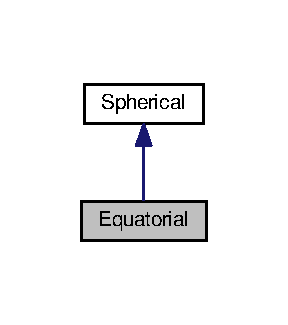
\includegraphics[width=138pt]{class_equatorial__inherit__graph}
\end{center}
\end{figure}


Collaboration diagram for Equatorial\-:\nopagebreak
\begin{figure}[H]
\begin{center}
\leavevmode
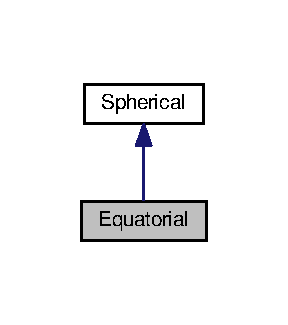
\includegraphics[width=138pt]{class_equatorial__coll__graph}
\end{center}
\end{figure}
\subsection*{Public Member Functions}
\begin{DoxyCompactItemize}
\item 
\hyperlink{class_equatorial_a8310993e702bce92cfd908751fb6d17c}{Equatorial} ()=default
\item 
\hyperlink{class_equatorial_a559465c0a50bd1d463a394eeb834bf04}{Equatorial} (array$<$ double, 3 $>$ pos)
\end{DoxyCompactItemize}
\subsection*{Additional Inherited Members}


\subsection{Detailed Description}


Definition at line 37 of file Spherical.\-hpp.



\subsection{Constructor \& Destructor Documentation}
\hypertarget{class_equatorial_a8310993e702bce92cfd908751fb6d17c}{\index{Equatorial@{Equatorial}!Equatorial@{Equatorial}}
\index{Equatorial@{Equatorial}!Equatorial@{Equatorial}}
\subsubsection[{Equatorial}]{\setlength{\rightskip}{0pt plus 5cm}Equatorial\-::\-Equatorial (
\begin{DoxyParamCaption}
{}
\end{DoxyParamCaption}
)\hspace{0.3cm}{\ttfamily [default]}}}\label{class_equatorial_a8310993e702bce92cfd908751fb6d17c}
\hypertarget{class_equatorial_a559465c0a50bd1d463a394eeb834bf04}{\index{Equatorial@{Equatorial}!Equatorial@{Equatorial}}
\index{Equatorial@{Equatorial}!Equatorial@{Equatorial}}
\subsubsection[{Equatorial}]{\setlength{\rightskip}{0pt plus 5cm}Equatorial\-::\-Equatorial (
\begin{DoxyParamCaption}
\item[{array$<$ double, 3 $>$}]{pos}
\end{DoxyParamCaption}
)}}\label{class_equatorial_a559465c0a50bd1d463a394eeb834bf04}


Definition at line 112 of file Spherical.\-cpp.



The documentation for this class was generated from the following files\-:\begin{DoxyCompactItemize}
\item 
/home/vish/code/trunk/cpp/libcarma/include/\hyperlink{_spherical_8hpp}{Spherical.\-hpp}\item 
/home/vish/code/trunk/cpp/libcarma/src/\hyperlink{_spherical_8cpp}{Spherical.\-cpp}\end{DoxyCompactItemize}

\hypertarget{class_galactic}{\section{Galactic Class Reference}
\label{class_galactic}\index{Galactic@{Galactic}}
}


{\ttfamily \#include $<$Spherical.\-hpp$>$}



Inheritance diagram for Galactic\-:\nopagebreak
\begin{figure}[H]
\begin{center}
\leavevmode
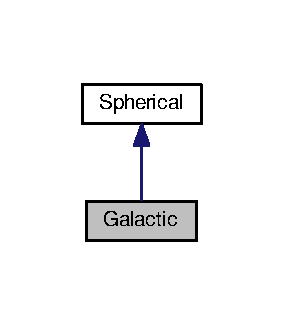
\includegraphics[width=136pt]{class_galactic__inherit__graph}
\end{center}
\end{figure}


Collaboration diagram for Galactic\-:\nopagebreak
\begin{figure}[H]
\begin{center}
\leavevmode
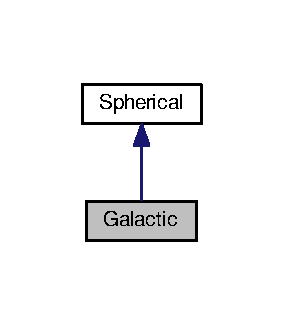
\includegraphics[width=136pt]{class_galactic__coll__graph}
\end{center}
\end{figure}
\subsection*{Public Member Functions}
\begin{DoxyCompactItemize}
\item 
\hyperlink{class_galactic_adb8910a11762d017934147c1105a2f25}{Galactic} ()=default
\item 
\hyperlink{class_galactic_ae554ae637bdabd965c41ce5ce05b8b8b}{Galactic} (array$<$ double, 3 $>$ pos)
\end{DoxyCompactItemize}
\subsection*{Additional Inherited Members}


\subsection{Detailed Description}


Definition at line 43 of file Spherical.\-hpp.



\subsection{Constructor \& Destructor Documentation}
\hypertarget{class_galactic_adb8910a11762d017934147c1105a2f25}{\index{Galactic@{Galactic}!Galactic@{Galactic}}
\index{Galactic@{Galactic}!Galactic@{Galactic}}
\subsubsection[{Galactic}]{\setlength{\rightskip}{0pt plus 5cm}Galactic\-::\-Galactic (
\begin{DoxyParamCaption}
{}
\end{DoxyParamCaption}
)\hspace{0.3cm}{\ttfamily [default]}}}\label{class_galactic_adb8910a11762d017934147c1105a2f25}
\hypertarget{class_galactic_ae554ae637bdabd965c41ce5ce05b8b8b}{\index{Galactic@{Galactic}!Galactic@{Galactic}}
\index{Galactic@{Galactic}!Galactic@{Galactic}}
\subsubsection[{Galactic}]{\setlength{\rightskip}{0pt plus 5cm}Galactic\-::\-Galactic (
\begin{DoxyParamCaption}
\item[{array$<$ double, 3 $>$}]{pos}
\end{DoxyParamCaption}
)}}\label{class_galactic_ae554ae637bdabd965c41ce5ce05b8b8b}


Definition at line 116 of file Spherical.\-cpp.



The documentation for this class was generated from the following files\-:\begin{DoxyCompactItemize}
\item 
/home/vish/code/trunk/cpp/libcarma/include/\hyperlink{_spherical_8hpp}{Spherical.\-hpp}\item 
/home/vish/code/trunk/cpp/libcarma/src/\hyperlink{_spherical_8cpp}{Spherical.\-cpp}\end{DoxyCompactItemize}

\hypertarget{struct_gauss_m_v}{\section{Gauss\-M\-V Struct Reference}
\label{struct_gauss_m_v}\index{Gauss\-M\-V@{Gauss\-M\-V}}
}


{\ttfamily \#include $<$Gauss\-M\-V.\-hpp$>$}

\subsection*{Public Attributes}
\begin{DoxyCompactItemize}
\item 
double $\ast$ \hyperlink{struct_gauss_m_v_ae45dad7a24aec8e56e0d2d9814a3f267}{mu}
\item 
double $\ast$ \hyperlink{struct_gauss_m_v_a4578d70691b74556849669fae207ff64}{var}
\end{DoxyCompactItemize}


\subsection{Detailed Description}


Definition at line 11 of file Gauss\-M\-V.\-hpp.



\subsection{Member Data Documentation}
\hypertarget{struct_gauss_m_v_ae45dad7a24aec8e56e0d2d9814a3f267}{\index{Gauss\-M\-V@{Gauss\-M\-V}!mu@{mu}}
\index{mu@{mu}!GaussMV@{Gauss\-M\-V}}
\subsubsection[{mu}]{\setlength{\rightskip}{0pt plus 5cm}double$\ast$ Gauss\-M\-V\-::mu}}\label{struct_gauss_m_v_ae45dad7a24aec8e56e0d2d9814a3f267}


Definition at line 12 of file Gauss\-M\-V.\-hpp.

\hypertarget{struct_gauss_m_v_a4578d70691b74556849669fae207ff64}{\index{Gauss\-M\-V@{Gauss\-M\-V}!var@{var}}
\index{var@{var}!GaussMV@{Gauss\-M\-V}}
\subsubsection[{var}]{\setlength{\rightskip}{0pt plus 5cm}double $\ast$ Gauss\-M\-V\-::var}}\label{struct_gauss_m_v_a4578d70691b74556849669fae207ff64}


Definition at line 12 of file Gauss\-M\-V.\-hpp.



The documentation for this struct was generated from the following file\-:\begin{DoxyCompactItemize}
\item 
/home/vish/code/trunk/cpp/libcarma/include/\hyperlink{_gauss_m_v_8hpp}{Gauss\-M\-V.\-hpp}\end{DoxyCompactItemize}

\hypertarget{class_kepler_obj}{\section{Kepler\-Obj Class Reference}
\label{class_kepler_obj}\index{Kepler\-Obj@{Kepler\-Obj}}
}


{\ttfamily \#include $<$Kepler.\-hpp$>$}



Inheritance diagram for Kepler\-Obj\-:\nopagebreak
\begin{figure}[H]
\begin{center}
\leavevmode
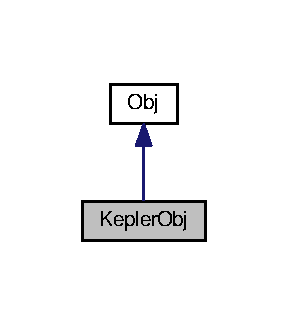
\includegraphics[width=138pt]{class_kepler_obj__inherit__graph}
\end{center}
\end{figure}


Collaboration diagram for Kepler\-Obj\-:\nopagebreak
\begin{figure}[H]
\begin{center}
\leavevmode
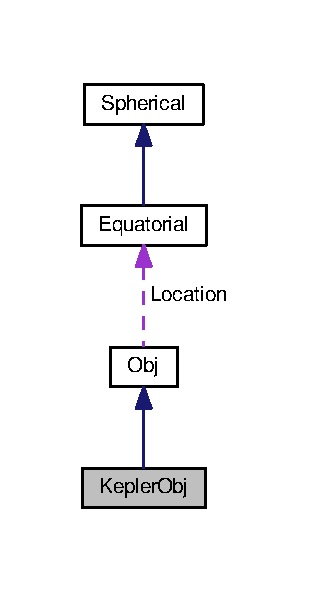
\includegraphics[width=149pt]{class_kepler_obj__coll__graph}
\end{center}
\end{figure}
\subsection*{Public Member Functions}
\begin{DoxyCompactItemize}
\item 
\hyperlink{class_kepler_obj_afd0b831e625b2c4f5c75c458a2dd0ba7}{Kepler\-Obj} ()=default
\item 
\hyperlink{class_kepler_obj_a6f5497c0170b840769e22e317332644e}{Kepler\-Obj} (string id, string path, \hyperlink{class_equatorial}{Equatorial} loc)
\item 
string \hyperlink{class_kepler_obj_a268fc8a6f87be9489c5ee4d52903fd2c}{get\-I\-D} ()
\item 
string \hyperlink{class_kepler_obj_a3e99e434a7328f45137b94ae9557ceeb}{get\-Path} ()
\item 
\hyperlink{class_equatorial}{Equatorial} \hyperlink{class_kepler_obj_ace9583f6845dc6db9e0e23ec60bb0c54}{get\-Location} ()
\item 
double \hyperlink{class_kepler_obj_aa39f1254aa63f9cec80061be6da46a58}{get\-Red\-Shift} ()
\item 
int \hyperlink{class_kepler_obj_acd3e416bd288f43a30a7b753a6697f99}{get\-Order} ()
\item 
void \hyperlink{class_kepler_obj_af7e062113cc6222956d892733b36142f}{set\-Order} (int ord)
\item 
int \hyperlink{class_kepler_obj_ad953af55b06af0234c68e54c6275d7e4}{get\-Num\-Cadences} ()
\item 
int \hyperlink{class_kepler_obj_a1980eedbf8b3b8c7e04b41dc887630f1}{get\-Num\-Lags} ()
\item 
int \hyperlink{class_kepler_obj_ad44d1900ee67daddc8d7c93887a05f46}{get\-Over\-Sample\-Factor} ()
\item 
void \hyperlink{class_kepler_obj_a8cf9e305908521eaf390f5dd96fe9b4a}{set\-Over\-Sample\-Factor} (int over\-Sample\-Factor)
\item 
int \hyperlink{class_kepler_obj_a37ec5e30230b9e91a9f4e54033097fc9}{get\-Num\-Quarters} ()
\item 
double \hyperlink{class_kepler_obj_a5fd1060cb4c3c1cbc804e0bf20eddfa0}{get\-Start\-Epoch} ()
\item 
double \hyperlink{class_kepler_obj_a195fb841c86bb6d947bcd9a7c45ec56e}{get\-Mean\-Flux} ()
\item 
int \hyperlink{class_kepler_obj_a8f53290957f8902ddb5668a21527e4ba}{get\-First\-Cadence} ()
\item 
int \hyperlink{class_kepler_obj_ad2c733e73ddd622f8c2b74b070ba9f51}{get\-Last\-Cadence} ()
\item 
void \hyperlink{class_kepler_obj_a7ac5a2d3bdaa7a41a39a238788f8a6fa}{set\-Frac\-H\-O\-S\-T} (double frac\-H\-O\-S\-T)
\item 
double \hyperlink{class_kepler_obj_a230eab3c510a51b2197cf6ec7e30fd75}{get\-Frac\-H\-O\-S\-T} ()
\item 
void \hyperlink{class_kepler_obj_a612da6fa87b8f97c4f161bc5f39fe9ea}{set\-Frac\-M\-I\-C} (double frac\-M\-I\-C)
\item 
double \hyperlink{class_kepler_obj_a0ff0576f717c68e5e4b9f0757c3f80f7}{get\-Frac\-M\-I\-C} ()
\item 
int \hyperlink{class_kepler_obj_a9dadabc2f3314221e358a3c056b22f21}{get\-Stage} ()
\item 
void \hyperlink{class_kepler_obj_afcd5f85bcd1f39d590d70e0dcdc1ee08}{set\-Stage} (int stage)
\item 
void \hyperlink{class_kepler_obj_ace628ec6c767aff9168497ec63984ccc}{set\-Num\-Sims\-S\-I} (int num\-Sims\-S\-I)
\item 
int \hyperlink{class_kepler_obj_ade4482c97b7fc9ea66ec8b94a289f881}{get\-Num\-Sims\-S\-I} ()
\item 
void \hyperlink{class_kepler_obj_a43d6d7205c8a92397558a97217511b62}{set\-Max\-Evals\-S\-I} (int max\-Evals\-S\-I)
\item 
int \hyperlink{class_kepler_obj_aa23b06e8009166f41be3885df24317d4}{get\-Max\-Evals\-S\-I} ()
\item 
void \hyperlink{class_kepler_obj_a3e6045761b050157a17fb578685bdd9a}{set\-F\-Tol\-S\-I} (double f\-Tol\-S\-I)
\item 
double \hyperlink{class_kepler_obj_a4fb09c27d3291bd40875d78cfdc2e80c}{get\-F\-Tol\-S\-I} ()
\item 
void \hyperlink{class_kepler_obj_a762cbe9392ac57bcb4fa64858826e1f1}{set\-Num\-Sims\-S\-I\-I} (int num\-Sims\-S\-I\-I)
\item 
int \hyperlink{class_kepler_obj_aa3cf9a27159e7e6a4035434c5e10d65b}{get\-Num\-Sims\-S\-I\-I} ()
\item 
void \hyperlink{class_kepler_obj_ab6eaf04d2a806c718a41c38a44af6190}{set\-Max\-Evals\-S\-I\-I} (int max\-Evals\-S\-I\-I)
\item 
int \hyperlink{class_kepler_obj_a5c3a7895c5a602b005bbb2042e1650e8}{get\-Max\-Evals\-S\-I\-I} ()
\item 
void \hyperlink{class_kepler_obj_a799a2b684a67435c404e6071af7b00f6}{set\-F\-Tol\-S\-I\-I} (double f\-Tol\-S\-I\-I)
\item 
double \hyperlink{class_kepler_obj_acbf137e5718db7b15f72c91fa4d2f726}{get\-F\-Tol\-S\-I\-I} ()
\item 
void \hyperlink{class_kepler_obj_a78ddbc7c63e7d698e968a65d04ed5ae1}{set\-Num\-Sims\-C\-S} (int num\-Sims\-C\-S)
\item 
int \hyperlink{class_kepler_obj_a70fe38e2ebdfda98be4284f00e6c4734}{get\-Num\-Sims\-C\-S} ()
\item 
void \hyperlink{class_kepler_obj_a00f426d160b0674bfe52d2f36014e465}{set\-Max\-Evals\-C\-S} ()
\item 
int \hyperlink{class_kepler_obj_adda2765461c9fe80a8427f39b8f841ed}{get\-Max\-Evals\-C\-S} ()
\item 
void \hyperlink{class_kepler_obj_a94b23d5f4fe9142053e2c0a8d5a7eab4}{set\-Num\-Chi\-Sq} (int num\-Chi\-Sq)
\item 
int \hyperlink{class_kepler_obj_a7c4abbe2e792cff003d957d9b631dc74}{get\-Num\-Chi\-Sq} ()
\item 
void \hyperlink{class_kepler_obj_afaefc71cee5ab1f7fed60366910b77d2}{set\-Num\-Seeds} (int num\-Seeds)
\item 
int \hyperlink{class_kepler_obj_aff16c04462b1714a474a1c2bb3be30ff}{get\-Num\-Seeds} ()
\item 
tuple$<$ vector$<$ array$<$ int, 2 $>$\\*
 $>$, vector$<$ array$<$ double, 5 $>$ $>$ $>$ \hyperlink{class_kepler_obj_a9162e912a70706492323c4a7b84e25a7}{get\-Data} ()
\item 
tuple$<$ vector$<$ array$<$ int, 2 $>$\\*
 $>$, vector$<$ array$<$ double, 5 $>$ $>$ $>$ \hyperlink{class_kepler_obj_ac372c45b9df44b41192324c50629dd92}{get\-Data} (int stitch\-Method)
\item 
tuple$<$ vector$<$ array$<$ int, 2 $>$\\*
 $>$, vector$<$ array$<$ double, 5 $>$ $>$ $>$ \hyperlink{class_kepler_obj_acb2e980082a9a943dbecb40cf4dcd0bb}{get\-Data} (bool force\-Calibrate, int stitch\-Method)
\item 
tuple$<$ vector$<$ array$<$ int, 2 $>$\\*
 $>$, vector$<$ array$<$ double, 5 $>$ $>$ $>$ \hyperlink{class_kepler_obj_a3f09ad774ae8ffad8936ff1c2f91bcbb}{get\-Data} (string \&file\-Name, bool cbv\-O\-Rpdc)
\item 
tuple$<$ vector$<$ array$<$ int, 2 $>$\\*
 $>$, vector$<$ array$<$ double, 5 $>$ $>$ $>$ \hyperlink{class_kepler_obj_af0c74aa514da769c45ddd1b5d6fa09d8}{get\-Data} (string \&filename, bool cbv\-O\-Rpdc, int stitch\-Method)
\item 
tuple$<$ vector$<$ array$<$ int, 2 $>$\\*
 $>$, vector$<$ array$<$ double, 5 $>$ $>$ $>$ \hyperlink{class_kepler_obj_a4f90cf9b7aa47fdaca37001c9032fea1}{get\-Data} (string \&file\-Name, bool cbv\-O\-Rpdc, bool force\-Calibrate, int stitch\-Method)
\item 
void \hyperlink{class_kepler_obj_a18ece34d36959a5eb0c75c34bdeea2ae}{set\-Properties} (const tuple$<$ vector$<$ array$<$ int, 2 $>$$>$, vector$<$ array$<$ double, 5 $>$$>$$>$ \&data\-Array)
\item 
void \hyperlink{class_kepler_obj_a0712485c7f8f87047dff986c06bca53e}{set\-Mask} (const tuple$<$ vector$<$ array$<$ int, 2 $>$$>$, vector$<$ array$<$ double, 5 $>$$>$$>$ \&data\-Array, double $\ast$mask)
\item 
vector$<$ unsigned int $>$ \hyperlink{class_kepler_obj_ab0d9b5872db2ceaf8a589da7a6c5b24a}{get\-Seeds} ()
\item 
vector$<$ unsigned int $>$ \hyperlink{class_kepler_obj_ad493b1e9867acac00840229d31b71e2a}{get\-Seeds} (int num\-Seeds\-Req)
\item 
int \hyperlink{class_kepler_obj_ac57d999ff4bdb6cbcfc710803d034cc1}{epoch\-Toindex} (double epoch)
\item 
double \hyperlink{class_kepler_obj_a7b822c1719305ecc53c4594fab113c99}{index\-Toepoch} (int index)
\item 
vector$<$ int $>$ \hyperlink{class_kepler_obj_a707be7b6de877f1d4a66f022f5f7b08e}{epoch\-Toindex} (vector$<$ double $>$ epoch\-List)
\item 
vector$<$ double $>$ \hyperlink{class_kepler_obj_a89d53cab1519c3cb5d337da37565b60d}{index\-Toepoch} (vector$<$ int $>$ index\-List)
\end{DoxyCompactItemize}
\subsection*{Additional Inherited Members}


\subsection{Detailed Description}


Definition at line 11 of file Kepler.\-hpp.



\subsection{Constructor \& Destructor Documentation}
\hypertarget{class_kepler_obj_afd0b831e625b2c4f5c75c458a2dd0ba7}{\index{Kepler\-Obj@{Kepler\-Obj}!Kepler\-Obj@{Kepler\-Obj}}
\index{Kepler\-Obj@{Kepler\-Obj}!KeplerObj@{Kepler\-Obj}}
\subsubsection[{Kepler\-Obj}]{\setlength{\rightskip}{0pt plus 5cm}Kepler\-Obj\-::\-Kepler\-Obj (
\begin{DoxyParamCaption}
{}
\end{DoxyParamCaption}
)\hspace{0.3cm}{\ttfamily [default]}}}\label{class_kepler_obj_afd0b831e625b2c4f5c75c458a2dd0ba7}
\hypertarget{class_kepler_obj_a6f5497c0170b840769e22e317332644e}{\index{Kepler\-Obj@{Kepler\-Obj}!Kepler\-Obj@{Kepler\-Obj}}
\index{Kepler\-Obj@{Kepler\-Obj}!KeplerObj@{Kepler\-Obj}}
\subsubsection[{Kepler\-Obj}]{\setlength{\rightskip}{0pt plus 5cm}Kepler\-Obj\-::\-Kepler\-Obj (
\begin{DoxyParamCaption}
\item[{string}]{id, }
\item[{string}]{path, }
\item[{{\bf Equatorial}}]{loc}
\end{DoxyParamCaption}
)}}\label{class_kepler_obj_a6f5497c0170b840769e22e317332644e}


Definition at line 23 of file Kepler.\-cpp.



\subsection{Member Function Documentation}
\hypertarget{class_kepler_obj_ac57d999ff4bdb6cbcfc710803d034cc1}{\index{Kepler\-Obj@{Kepler\-Obj}!epoch\-Toindex@{epoch\-Toindex}}
\index{epoch\-Toindex@{epoch\-Toindex}!KeplerObj@{Kepler\-Obj}}
\subsubsection[{epoch\-Toindex}]{\setlength{\rightskip}{0pt plus 5cm}int Kepler\-Obj\-::epoch\-Toindex (
\begin{DoxyParamCaption}
\item[{double}]{epoch}
\end{DoxyParamCaption}
)}}\label{class_kepler_obj_ac57d999ff4bdb6cbcfc710803d034cc1}


Definition at line 822 of file Kepler.\-cpp.

\hypertarget{class_kepler_obj_a707be7b6de877f1d4a66f022f5f7b08e}{\index{Kepler\-Obj@{Kepler\-Obj}!epoch\-Toindex@{epoch\-Toindex}}
\index{epoch\-Toindex@{epoch\-Toindex}!KeplerObj@{Kepler\-Obj}}
\subsubsection[{epoch\-Toindex}]{\setlength{\rightskip}{0pt plus 5cm}vector$<$ int $>$ Kepler\-Obj\-::epoch\-Toindex (
\begin{DoxyParamCaption}
\item[{vector$<$ double $>$}]{epoch\-List}
\end{DoxyParamCaption}
)}}\label{class_kepler_obj_a707be7b6de877f1d4a66f022f5f7b08e}


Definition at line 832 of file Kepler.\-cpp.

\hypertarget{class_kepler_obj_a9162e912a70706492323c4a7b84e25a7}{\index{Kepler\-Obj@{Kepler\-Obj}!get\-Data@{get\-Data}}
\index{get\-Data@{get\-Data}!KeplerObj@{Kepler\-Obj}}
\subsubsection[{get\-Data}]{\setlength{\rightskip}{0pt plus 5cm}tuple$<$ vector$<$ array$<$ int, 2 $>$ $>$, vector$<$ array$<$ double, 5 $>$ $>$ $>$ Kepler\-Obj\-::get\-Data (
\begin{DoxyParamCaption}
{}
\end{DoxyParamCaption}
)}}\label{class_kepler_obj_a9162e912a70706492323c4a7b84e25a7}


Definition at line 559 of file Kepler.\-cpp.



Here is the caller graph for this function\-:\nopagebreak
\begin{figure}[H]
\begin{center}
\leavevmode
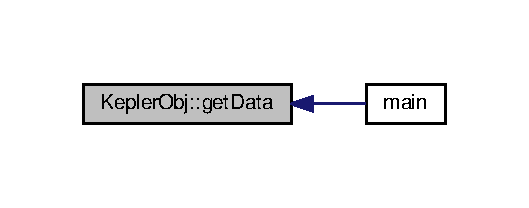
\includegraphics[width=254pt]{class_kepler_obj_a9162e912a70706492323c4a7b84e25a7_icgraph}
\end{center}
\end{figure}


\hypertarget{class_kepler_obj_ac372c45b9df44b41192324c50629dd92}{\index{Kepler\-Obj@{Kepler\-Obj}!get\-Data@{get\-Data}}
\index{get\-Data@{get\-Data}!KeplerObj@{Kepler\-Obj}}
\subsubsection[{get\-Data}]{\setlength{\rightskip}{0pt plus 5cm}tuple$<$ vector$<$ array$<$ int, 2 $>$ $>$, vector$<$ array$<$ double, 5 $>$ $>$ $>$ Kepler\-Obj\-::get\-Data (
\begin{DoxyParamCaption}
\item[{int}]{stitch\-Method}
\end{DoxyParamCaption}
)}}\label{class_kepler_obj_ac372c45b9df44b41192324c50629dd92}


Definition at line 565 of file Kepler.\-cpp.

\hypertarget{class_kepler_obj_acb2e980082a9a943dbecb40cf4dcd0bb}{\index{Kepler\-Obj@{Kepler\-Obj}!get\-Data@{get\-Data}}
\index{get\-Data@{get\-Data}!KeplerObj@{Kepler\-Obj}}
\subsubsection[{get\-Data}]{\setlength{\rightskip}{0pt plus 5cm}tuple$<$ vector$<$ array$<$ int, 2 $>$ $>$, vector$<$ array$<$ double, 5 $>$ $>$ $>$ Kepler\-Obj\-::get\-Data (
\begin{DoxyParamCaption}
\item[{bool}]{force\-Calibrate, }
\item[{int}]{stitch\-Method}
\end{DoxyParamCaption}
)}}\label{class_kepler_obj_acb2e980082a9a943dbecb40cf4dcd0bb}


Definition at line 571 of file Kepler.\-cpp.



Here is the call graph for this function\-:\nopagebreak
\begin{figure}[H]
\begin{center}
\leavevmode
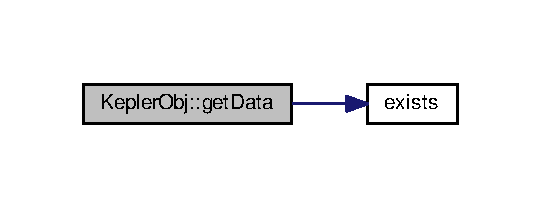
\includegraphics[width=260pt]{class_kepler_obj_acb2e980082a9a943dbecb40cf4dcd0bb_cgraph}
\end{center}
\end{figure}


\hypertarget{class_kepler_obj_a3f09ad774ae8ffad8936ff1c2f91bcbb}{\index{Kepler\-Obj@{Kepler\-Obj}!get\-Data@{get\-Data}}
\index{get\-Data@{get\-Data}!KeplerObj@{Kepler\-Obj}}
\subsubsection[{get\-Data}]{\setlength{\rightskip}{0pt plus 5cm}tuple$<$ vector$<$ array$<$ int, 2 $>$ $>$, vector$<$ array$<$ double, 5 $>$ $>$ $>$ Kepler\-Obj\-::get\-Data (
\begin{DoxyParamCaption}
\item[{string \&}]{file\-Name, }
\item[{bool}]{cbv\-O\-Rpdc}
\end{DoxyParamCaption}
)}}\label{class_kepler_obj_a3f09ad774ae8ffad8936ff1c2f91bcbb}


Definition at line 727 of file Kepler.\-cpp.

\hypertarget{class_kepler_obj_af0c74aa514da769c45ddd1b5d6fa09d8}{\index{Kepler\-Obj@{Kepler\-Obj}!get\-Data@{get\-Data}}
\index{get\-Data@{get\-Data}!KeplerObj@{Kepler\-Obj}}
\subsubsection[{get\-Data}]{\setlength{\rightskip}{0pt plus 5cm}tuple$<$ vector$<$ array$<$ int, 2 $>$ $>$, vector$<$ array$<$ double, 5 $>$ $>$ $>$ Kepler\-Obj\-::get\-Data (
\begin{DoxyParamCaption}
\item[{string \&}]{filename, }
\item[{bool}]{cbv\-O\-Rpdc, }
\item[{int}]{stitch\-Method}
\end{DoxyParamCaption}
)}}\label{class_kepler_obj_af0c74aa514da769c45ddd1b5d6fa09d8}


Definition at line 733 of file Kepler.\-cpp.

\hypertarget{class_kepler_obj_a4f90cf9b7aa47fdaca37001c9032fea1}{\index{Kepler\-Obj@{Kepler\-Obj}!get\-Data@{get\-Data}}
\index{get\-Data@{get\-Data}!KeplerObj@{Kepler\-Obj}}
\subsubsection[{get\-Data}]{\setlength{\rightskip}{0pt plus 5cm}tuple$<$ vector$<$ array$<$ int, 2 $>$ $>$, vector$<$ array$<$ double, 5 $>$ $>$ $>$ Kepler\-Obj\-::get\-Data (
\begin{DoxyParamCaption}
\item[{string \&}]{file\-Name, }
\item[{bool}]{cbv\-O\-Rpdc, }
\item[{bool}]{force\-Calibrate, }
\item[{int}]{stitch\-Method}
\end{DoxyParamCaption}
)}}\label{class_kepler_obj_a4f90cf9b7aa47fdaca37001c9032fea1}


Definition at line 649 of file Kepler.\-cpp.



Here is the call graph for this function\-:\nopagebreak
\begin{figure}[H]
\begin{center}
\leavevmode
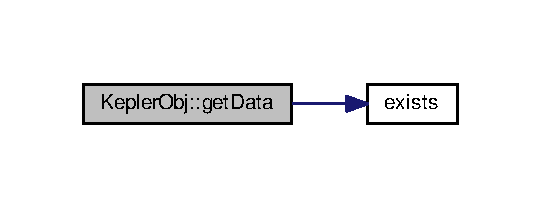
\includegraphics[width=260pt]{class_kepler_obj_a4f90cf9b7aa47fdaca37001c9032fea1_cgraph}
\end{center}
\end{figure}


\hypertarget{class_kepler_obj_a8f53290957f8902ddb5668a21527e4ba}{\index{Kepler\-Obj@{Kepler\-Obj}!get\-First\-Cadence@{get\-First\-Cadence}}
\index{get\-First\-Cadence@{get\-First\-Cadence}!KeplerObj@{Kepler\-Obj}}
\subsubsection[{get\-First\-Cadence}]{\setlength{\rightskip}{0pt plus 5cm}int Kepler\-Obj\-::get\-First\-Cadence (
\begin{DoxyParamCaption}
{}
\end{DoxyParamCaption}
)}}\label{class_kepler_obj_a8f53290957f8902ddb5668a21527e4ba}


Definition at line 739 of file Kepler.\-cpp.



Here is the caller graph for this function\-:\nopagebreak
\begin{figure}[H]
\begin{center}
\leavevmode
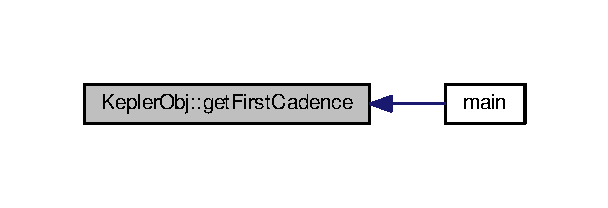
\includegraphics[width=292pt]{class_kepler_obj_a8f53290957f8902ddb5668a21527e4ba_icgraph}
\end{center}
\end{figure}


\hypertarget{class_kepler_obj_a230eab3c510a51b2197cf6ec7e30fd75}{\index{Kepler\-Obj@{Kepler\-Obj}!get\-Frac\-H\-O\-S\-T@{get\-Frac\-H\-O\-S\-T}}
\index{get\-Frac\-H\-O\-S\-T@{get\-Frac\-H\-O\-S\-T}!KeplerObj@{Kepler\-Obj}}
\subsubsection[{get\-Frac\-H\-O\-S\-T}]{\setlength{\rightskip}{0pt plus 5cm}double Kepler\-Obj\-::get\-Frac\-H\-O\-S\-T (
\begin{DoxyParamCaption}
{}
\end{DoxyParamCaption}
)}}\label{class_kepler_obj_a230eab3c510a51b2197cf6ec7e30fd75}


Definition at line 98 of file Kepler.\-cpp.

\hypertarget{class_kepler_obj_a0ff0576f717c68e5e4b9f0757c3f80f7}{\index{Kepler\-Obj@{Kepler\-Obj}!get\-Frac\-M\-I\-C@{get\-Frac\-M\-I\-C}}
\index{get\-Frac\-M\-I\-C@{get\-Frac\-M\-I\-C}!KeplerObj@{Kepler\-Obj}}
\subsubsection[{get\-Frac\-M\-I\-C}]{\setlength{\rightskip}{0pt plus 5cm}double Kepler\-Obj\-::get\-Frac\-M\-I\-C (
\begin{DoxyParamCaption}
{}
\end{DoxyParamCaption}
)}}\label{class_kepler_obj_a0ff0576f717c68e5e4b9f0757c3f80f7}


Definition at line 106 of file Kepler.\-cpp.

\hypertarget{class_kepler_obj_a4fb09c27d3291bd40875d78cfdc2e80c}{\index{Kepler\-Obj@{Kepler\-Obj}!get\-F\-Tol\-S\-I@{get\-F\-Tol\-S\-I}}
\index{get\-F\-Tol\-S\-I@{get\-F\-Tol\-S\-I}!KeplerObj@{Kepler\-Obj}}
\subsubsection[{get\-F\-Tol\-S\-I}]{\setlength{\rightskip}{0pt plus 5cm}double Kepler\-Obj\-::get\-F\-Tol\-S\-I (
\begin{DoxyParamCaption}
{}
\end{DoxyParamCaption}
)}}\label{class_kepler_obj_a4fb09c27d3291bd40875d78cfdc2e80c}


Definition at line 142 of file Kepler.\-cpp.

\hypertarget{class_kepler_obj_acbf137e5718db7b15f72c91fa4d2f726}{\index{Kepler\-Obj@{Kepler\-Obj}!get\-F\-Tol\-S\-I\-I@{get\-F\-Tol\-S\-I\-I}}
\index{get\-F\-Tol\-S\-I\-I@{get\-F\-Tol\-S\-I\-I}!KeplerObj@{Kepler\-Obj}}
\subsubsection[{get\-F\-Tol\-S\-I\-I}]{\setlength{\rightskip}{0pt plus 5cm}double Kepler\-Obj\-::get\-F\-Tol\-S\-I\-I (
\begin{DoxyParamCaption}
{}
\end{DoxyParamCaption}
)}}\label{class_kepler_obj_acbf137e5718db7b15f72c91fa4d2f726}


Definition at line 166 of file Kepler.\-cpp.

\hypertarget{class_kepler_obj_a268fc8a6f87be9489c5ee4d52903fd2c}{\index{Kepler\-Obj@{Kepler\-Obj}!get\-I\-D@{get\-I\-D}}
\index{get\-I\-D@{get\-I\-D}!KeplerObj@{Kepler\-Obj}}
\subsubsection[{get\-I\-D}]{\setlength{\rightskip}{0pt plus 5cm}string Kepler\-Obj\-::get\-I\-D (
\begin{DoxyParamCaption}
{}
\end{DoxyParamCaption}
)}}\label{class_kepler_obj_a268fc8a6f87be9489c5ee4d52903fd2c}


Definition at line 58 of file Kepler.\-cpp.

\hypertarget{class_kepler_obj_ad2c733e73ddd622f8c2b74b070ba9f51}{\index{Kepler\-Obj@{Kepler\-Obj}!get\-Last\-Cadence@{get\-Last\-Cadence}}
\index{get\-Last\-Cadence@{get\-Last\-Cadence}!KeplerObj@{Kepler\-Obj}}
\subsubsection[{get\-Last\-Cadence}]{\setlength{\rightskip}{0pt plus 5cm}int Kepler\-Obj\-::get\-Last\-Cadence (
\begin{DoxyParamCaption}
{}
\end{DoxyParamCaption}
)}}\label{class_kepler_obj_ad2c733e73ddd622f8c2b74b070ba9f51}


Definition at line 743 of file Kepler.\-cpp.



Here is the caller graph for this function\-:\nopagebreak
\begin{figure}[H]
\begin{center}
\leavevmode
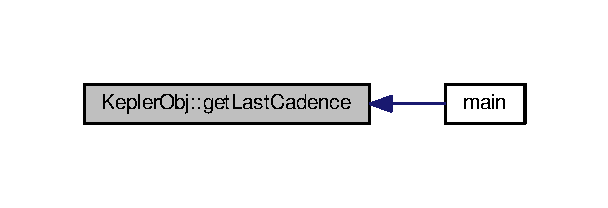
\includegraphics[width=292pt]{class_kepler_obj_ad2c733e73ddd622f8c2b74b070ba9f51_icgraph}
\end{center}
\end{figure}


\hypertarget{class_kepler_obj_ace9583f6845dc6db9e0e23ec60bb0c54}{\index{Kepler\-Obj@{Kepler\-Obj}!get\-Location@{get\-Location}}
\index{get\-Location@{get\-Location}!KeplerObj@{Kepler\-Obj}}
\subsubsection[{get\-Location}]{\setlength{\rightskip}{0pt plus 5cm}{\bf Equatorial} Kepler\-Obj\-::get\-Location (
\begin{DoxyParamCaption}
{}
\end{DoxyParamCaption}
)}}\label{class_kepler_obj_ace9583f6845dc6db9e0e23ec60bb0c54}


Definition at line 66 of file Kepler.\-cpp.

\hypertarget{class_kepler_obj_adda2765461c9fe80a8427f39b8f841ed}{\index{Kepler\-Obj@{Kepler\-Obj}!get\-Max\-Evals\-C\-S@{get\-Max\-Evals\-C\-S}}
\index{get\-Max\-Evals\-C\-S@{get\-Max\-Evals\-C\-S}!KeplerObj@{Kepler\-Obj}}
\subsubsection[{get\-Max\-Evals\-C\-S}]{\setlength{\rightskip}{0pt plus 5cm}int Kepler\-Obj\-::get\-Max\-Evals\-C\-S (
\begin{DoxyParamCaption}
{}
\end{DoxyParamCaption}
)}}\label{class_kepler_obj_adda2765461c9fe80a8427f39b8f841ed}


Definition at line 182 of file Kepler.\-cpp.

\hypertarget{class_kepler_obj_aa23b06e8009166f41be3885df24317d4}{\index{Kepler\-Obj@{Kepler\-Obj}!get\-Max\-Evals\-S\-I@{get\-Max\-Evals\-S\-I}}
\index{get\-Max\-Evals\-S\-I@{get\-Max\-Evals\-S\-I}!KeplerObj@{Kepler\-Obj}}
\subsubsection[{get\-Max\-Evals\-S\-I}]{\setlength{\rightskip}{0pt plus 5cm}int Kepler\-Obj\-::get\-Max\-Evals\-S\-I (
\begin{DoxyParamCaption}
{}
\end{DoxyParamCaption}
)}}\label{class_kepler_obj_aa23b06e8009166f41be3885df24317d4}


Definition at line 134 of file Kepler.\-cpp.

\hypertarget{class_kepler_obj_a5c3a7895c5a602b005bbb2042e1650e8}{\index{Kepler\-Obj@{Kepler\-Obj}!get\-Max\-Evals\-S\-I\-I@{get\-Max\-Evals\-S\-I\-I}}
\index{get\-Max\-Evals\-S\-I\-I@{get\-Max\-Evals\-S\-I\-I}!KeplerObj@{Kepler\-Obj}}
\subsubsection[{get\-Max\-Evals\-S\-I\-I}]{\setlength{\rightskip}{0pt plus 5cm}int Kepler\-Obj\-::get\-Max\-Evals\-S\-I\-I (
\begin{DoxyParamCaption}
{}
\end{DoxyParamCaption}
)}}\label{class_kepler_obj_a5c3a7895c5a602b005bbb2042e1650e8}


Definition at line 158 of file Kepler.\-cpp.

\hypertarget{class_kepler_obj_a195fb841c86bb6d947bcd9a7c45ec56e}{\index{Kepler\-Obj@{Kepler\-Obj}!get\-Mean\-Flux@{get\-Mean\-Flux}}
\index{get\-Mean\-Flux@{get\-Mean\-Flux}!KeplerObj@{Kepler\-Obj}}
\subsubsection[{get\-Mean\-Flux}]{\setlength{\rightskip}{0pt plus 5cm}double Kepler\-Obj\-::get\-Mean\-Flux (
\begin{DoxyParamCaption}
{}
\end{DoxyParamCaption}
)}}\label{class_kepler_obj_a195fb841c86bb6d947bcd9a7c45ec56e}


Definition at line 206 of file Kepler.\-cpp.

\hypertarget{class_kepler_obj_ad953af55b06af0234c68e54c6275d7e4}{\index{Kepler\-Obj@{Kepler\-Obj}!get\-Num\-Cadences@{get\-Num\-Cadences}}
\index{get\-Num\-Cadences@{get\-Num\-Cadences}!KeplerObj@{Kepler\-Obj}}
\subsubsection[{get\-Num\-Cadences}]{\setlength{\rightskip}{0pt plus 5cm}int Kepler\-Obj\-::get\-Num\-Cadences (
\begin{DoxyParamCaption}
{}
\end{DoxyParamCaption}
)}}\label{class_kepler_obj_ad953af55b06af0234c68e54c6275d7e4}


Definition at line 82 of file Kepler.\-cpp.



Here is the caller graph for this function\-:\nopagebreak
\begin{figure}[H]
\begin{center}
\leavevmode
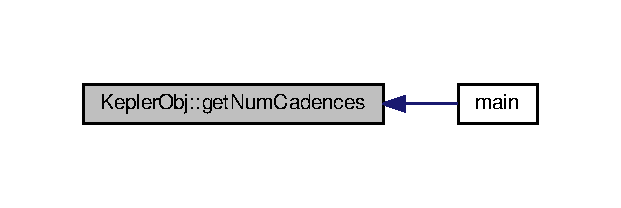
\includegraphics[width=298pt]{class_kepler_obj_ad953af55b06af0234c68e54c6275d7e4_icgraph}
\end{center}
\end{figure}


\hypertarget{class_kepler_obj_a7c4abbe2e792cff003d957d9b631dc74}{\index{Kepler\-Obj@{Kepler\-Obj}!get\-Num\-Chi\-Sq@{get\-Num\-Chi\-Sq}}
\index{get\-Num\-Chi\-Sq@{get\-Num\-Chi\-Sq}!KeplerObj@{Kepler\-Obj}}
\subsubsection[{get\-Num\-Chi\-Sq}]{\setlength{\rightskip}{0pt plus 5cm}int Kepler\-Obj\-::get\-Num\-Chi\-Sq (
\begin{DoxyParamCaption}
{}
\end{DoxyParamCaption}
)}}\label{class_kepler_obj_a7c4abbe2e792cff003d957d9b631dc74}


Definition at line 186 of file Kepler.\-cpp.

\hypertarget{class_kepler_obj_a1980eedbf8b3b8c7e04b41dc887630f1}{\index{Kepler\-Obj@{Kepler\-Obj}!get\-Num\-Lags@{get\-Num\-Lags}}
\index{get\-Num\-Lags@{get\-Num\-Lags}!KeplerObj@{Kepler\-Obj}}
\subsubsection[{get\-Num\-Lags}]{\setlength{\rightskip}{0pt plus 5cm}int Kepler\-Obj\-::get\-Num\-Lags (
\begin{DoxyParamCaption}
{}
\end{DoxyParamCaption}
)}}\label{class_kepler_obj_a1980eedbf8b3b8c7e04b41dc887630f1}


Definition at line 86 of file Kepler.\-cpp.

\hypertarget{class_kepler_obj_a37ec5e30230b9e91a9f4e54033097fc9}{\index{Kepler\-Obj@{Kepler\-Obj}!get\-Num\-Quarters@{get\-Num\-Quarters}}
\index{get\-Num\-Quarters@{get\-Num\-Quarters}!KeplerObj@{Kepler\-Obj}}
\subsubsection[{get\-Num\-Quarters}]{\setlength{\rightskip}{0pt plus 5cm}int Kepler\-Obj\-::get\-Num\-Quarters (
\begin{DoxyParamCaption}
{}
\end{DoxyParamCaption}
)}}\label{class_kepler_obj_a37ec5e30230b9e91a9f4e54033097fc9}


Definition at line 202 of file Kepler.\-cpp.

\hypertarget{class_kepler_obj_aff16c04462b1714a474a1c2bb3be30ff}{\index{Kepler\-Obj@{Kepler\-Obj}!get\-Num\-Seeds@{get\-Num\-Seeds}}
\index{get\-Num\-Seeds@{get\-Num\-Seeds}!KeplerObj@{Kepler\-Obj}}
\subsubsection[{get\-Num\-Seeds}]{\setlength{\rightskip}{0pt plus 5cm}int Kepler\-Obj\-::get\-Num\-Seeds (
\begin{DoxyParamCaption}
{}
\end{DoxyParamCaption}
)}}\label{class_kepler_obj_aff16c04462b1714a474a1c2bb3be30ff}


Definition at line 194 of file Kepler.\-cpp.

\hypertarget{class_kepler_obj_a70fe38e2ebdfda98be4284f00e6c4734}{\index{Kepler\-Obj@{Kepler\-Obj}!get\-Num\-Sims\-C\-S@{get\-Num\-Sims\-C\-S}}
\index{get\-Num\-Sims\-C\-S@{get\-Num\-Sims\-C\-S}!KeplerObj@{Kepler\-Obj}}
\subsubsection[{get\-Num\-Sims\-C\-S}]{\setlength{\rightskip}{0pt plus 5cm}int Kepler\-Obj\-::get\-Num\-Sims\-C\-S (
\begin{DoxyParamCaption}
{}
\end{DoxyParamCaption}
)}}\label{class_kepler_obj_a70fe38e2ebdfda98be4284f00e6c4734}


Definition at line 170 of file Kepler.\-cpp.

\hypertarget{class_kepler_obj_ade4482c97b7fc9ea66ec8b94a289f881}{\index{Kepler\-Obj@{Kepler\-Obj}!get\-Num\-Sims\-S\-I@{get\-Num\-Sims\-S\-I}}
\index{get\-Num\-Sims\-S\-I@{get\-Num\-Sims\-S\-I}!KeplerObj@{Kepler\-Obj}}
\subsubsection[{get\-Num\-Sims\-S\-I}]{\setlength{\rightskip}{0pt plus 5cm}int Kepler\-Obj\-::get\-Num\-Sims\-S\-I (
\begin{DoxyParamCaption}
{}
\end{DoxyParamCaption}
)}}\label{class_kepler_obj_ade4482c97b7fc9ea66ec8b94a289f881}


Definition at line 122 of file Kepler.\-cpp.

\hypertarget{class_kepler_obj_aa3cf9a27159e7e6a4035434c5e10d65b}{\index{Kepler\-Obj@{Kepler\-Obj}!get\-Num\-Sims\-S\-I\-I@{get\-Num\-Sims\-S\-I\-I}}
\index{get\-Num\-Sims\-S\-I\-I@{get\-Num\-Sims\-S\-I\-I}!KeplerObj@{Kepler\-Obj}}
\subsubsection[{get\-Num\-Sims\-S\-I\-I}]{\setlength{\rightskip}{0pt plus 5cm}int Kepler\-Obj\-::get\-Num\-Sims\-S\-I\-I (
\begin{DoxyParamCaption}
{}
\end{DoxyParamCaption}
)}}\label{class_kepler_obj_aa3cf9a27159e7e6a4035434c5e10d65b}


Definition at line 146 of file Kepler.\-cpp.

\hypertarget{class_kepler_obj_acd3e416bd288f43a30a7b753a6697f99}{\index{Kepler\-Obj@{Kepler\-Obj}!get\-Order@{get\-Order}}
\index{get\-Order@{get\-Order}!KeplerObj@{Kepler\-Obj}}
\subsubsection[{get\-Order}]{\setlength{\rightskip}{0pt plus 5cm}int Kepler\-Obj\-::get\-Order (
\begin{DoxyParamCaption}
{}
\end{DoxyParamCaption}
)}}\label{class_kepler_obj_acd3e416bd288f43a30a7b753a6697f99}


Definition at line 74 of file Kepler.\-cpp.

\hypertarget{class_kepler_obj_ad44d1900ee67daddc8d7c93887a05f46}{\index{Kepler\-Obj@{Kepler\-Obj}!get\-Over\-Sample\-Factor@{get\-Over\-Sample\-Factor}}
\index{get\-Over\-Sample\-Factor@{get\-Over\-Sample\-Factor}!KeplerObj@{Kepler\-Obj}}
\subsubsection[{get\-Over\-Sample\-Factor}]{\setlength{\rightskip}{0pt plus 5cm}int Kepler\-Obj\-::get\-Over\-Sample\-Factor (
\begin{DoxyParamCaption}
{}
\end{DoxyParamCaption}
)}}\label{class_kepler_obj_ad44d1900ee67daddc8d7c93887a05f46}


Definition at line 90 of file Kepler.\-cpp.

\hypertarget{class_kepler_obj_a3e99e434a7328f45137b94ae9557ceeb}{\index{Kepler\-Obj@{Kepler\-Obj}!get\-Path@{get\-Path}}
\index{get\-Path@{get\-Path}!KeplerObj@{Kepler\-Obj}}
\subsubsection[{get\-Path}]{\setlength{\rightskip}{0pt plus 5cm}string Kepler\-Obj\-::get\-Path (
\begin{DoxyParamCaption}
{}
\end{DoxyParamCaption}
)}}\label{class_kepler_obj_a3e99e434a7328f45137b94ae9557ceeb}


Definition at line 62 of file Kepler.\-cpp.

\hypertarget{class_kepler_obj_aa39f1254aa63f9cec80061be6da46a58}{\index{Kepler\-Obj@{Kepler\-Obj}!get\-Red\-Shift@{get\-Red\-Shift}}
\index{get\-Red\-Shift@{get\-Red\-Shift}!KeplerObj@{Kepler\-Obj}}
\subsubsection[{get\-Red\-Shift}]{\setlength{\rightskip}{0pt plus 5cm}double Kepler\-Obj\-::get\-Red\-Shift (
\begin{DoxyParamCaption}
{}
\end{DoxyParamCaption}
)}}\label{class_kepler_obj_aa39f1254aa63f9cec80061be6da46a58}


Definition at line 70 of file Kepler.\-cpp.

\hypertarget{class_kepler_obj_ab0d9b5872db2ceaf8a589da7a6c5b24a}{\index{Kepler\-Obj@{Kepler\-Obj}!get\-Seeds@{get\-Seeds}}
\index{get\-Seeds@{get\-Seeds}!KeplerObj@{Kepler\-Obj}}
\subsubsection[{get\-Seeds}]{\setlength{\rightskip}{0pt plus 5cm}vector$<$ unsigned int $>$ Kepler\-Obj\-::get\-Seeds (
\begin{DoxyParamCaption}
{}
\end{DoxyParamCaption}
)}}\label{class_kepler_obj_ab0d9b5872db2ceaf8a589da7a6c5b24a}


Definition at line 770 of file Kepler.\-cpp.



Here is the call graph for this function\-:\nopagebreak
\begin{figure}[H]
\begin{center}
\leavevmode
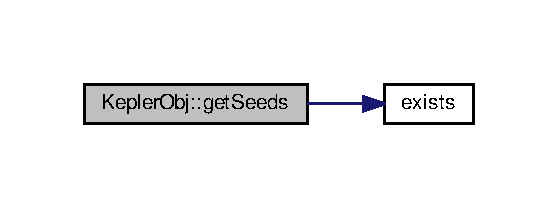
\includegraphics[width=268pt]{class_kepler_obj_ab0d9b5872db2ceaf8a589da7a6c5b24a_cgraph}
\end{center}
\end{figure}


\hypertarget{class_kepler_obj_ad493b1e9867acac00840229d31b71e2a}{\index{Kepler\-Obj@{Kepler\-Obj}!get\-Seeds@{get\-Seeds}}
\index{get\-Seeds@{get\-Seeds}!KeplerObj@{Kepler\-Obj}}
\subsubsection[{get\-Seeds}]{\setlength{\rightskip}{0pt plus 5cm}vector$<$ unsigned int $>$ Kepler\-Obj\-::get\-Seeds (
\begin{DoxyParamCaption}
\item[{int}]{num\-Seeds\-Req}
\end{DoxyParamCaption}
)}}\label{class_kepler_obj_ad493b1e9867acac00840229d31b71e2a}


Definition at line 794 of file Kepler.\-cpp.



Here is the call graph for this function\-:\nopagebreak
\begin{figure}[H]
\begin{center}
\leavevmode
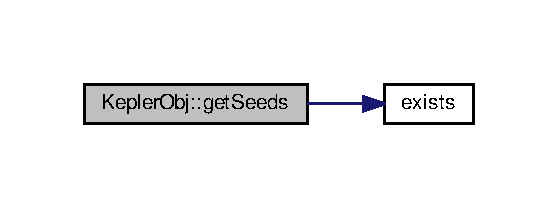
\includegraphics[width=268pt]{class_kepler_obj_ad493b1e9867acac00840229d31b71e2a_cgraph}
\end{center}
\end{figure}


\hypertarget{class_kepler_obj_a9dadabc2f3314221e358a3c056b22f21}{\index{Kepler\-Obj@{Kepler\-Obj}!get\-Stage@{get\-Stage}}
\index{get\-Stage@{get\-Stage}!KeplerObj@{Kepler\-Obj}}
\subsubsection[{get\-Stage}]{\setlength{\rightskip}{0pt plus 5cm}int Kepler\-Obj\-::get\-Stage (
\begin{DoxyParamCaption}
{}
\end{DoxyParamCaption}
)}}\label{class_kepler_obj_a9dadabc2f3314221e358a3c056b22f21}


Definition at line 114 of file Kepler.\-cpp.

\hypertarget{class_kepler_obj_a5fd1060cb4c3c1cbc804e0bf20eddfa0}{\index{Kepler\-Obj@{Kepler\-Obj}!get\-Start\-Epoch@{get\-Start\-Epoch}}
\index{get\-Start\-Epoch@{get\-Start\-Epoch}!KeplerObj@{Kepler\-Obj}}
\subsubsection[{get\-Start\-Epoch}]{\setlength{\rightskip}{0pt plus 5cm}double Kepler\-Obj\-::get\-Start\-Epoch (
\begin{DoxyParamCaption}
{}
\end{DoxyParamCaption}
)}}\label{class_kepler_obj_a5fd1060cb4c3c1cbc804e0bf20eddfa0}


Definition at line 210 of file Kepler.\-cpp.

\hypertarget{class_kepler_obj_a7b822c1719305ecc53c4594fab113c99}{\index{Kepler\-Obj@{Kepler\-Obj}!index\-Toepoch@{index\-Toepoch}}
\index{index\-Toepoch@{index\-Toepoch}!KeplerObj@{Kepler\-Obj}}
\subsubsection[{index\-Toepoch}]{\setlength{\rightskip}{0pt plus 5cm}double Kepler\-Obj\-::index\-Toepoch (
\begin{DoxyParamCaption}
\item[{int}]{index}
\end{DoxyParamCaption}
)}}\label{class_kepler_obj_a7b822c1719305ecc53c4594fab113c99}


Definition at line 827 of file Kepler.\-cpp.

\hypertarget{class_kepler_obj_a89d53cab1519c3cb5d337da37565b60d}{\index{Kepler\-Obj@{Kepler\-Obj}!index\-Toepoch@{index\-Toepoch}}
\index{index\-Toepoch@{index\-Toepoch}!KeplerObj@{Kepler\-Obj}}
\subsubsection[{index\-Toepoch}]{\setlength{\rightskip}{0pt plus 5cm}vector$<$ double $>$ Kepler\-Obj\-::index\-Toepoch (
\begin{DoxyParamCaption}
\item[{vector$<$ int $>$}]{index\-List}
\end{DoxyParamCaption}
)}}\label{class_kepler_obj_a89d53cab1519c3cb5d337da37565b60d}


Definition at line 842 of file Kepler.\-cpp.

\hypertarget{class_kepler_obj_a7ac5a2d3bdaa7a41a39a238788f8a6fa}{\index{Kepler\-Obj@{Kepler\-Obj}!set\-Frac\-H\-O\-S\-T@{set\-Frac\-H\-O\-S\-T}}
\index{set\-Frac\-H\-O\-S\-T@{set\-Frac\-H\-O\-S\-T}!KeplerObj@{Kepler\-Obj}}
\subsubsection[{set\-Frac\-H\-O\-S\-T}]{\setlength{\rightskip}{0pt plus 5cm}void Kepler\-Obj\-::set\-Frac\-H\-O\-S\-T (
\begin{DoxyParamCaption}
\item[{double}]{frac\-H\-O\-S\-T}
\end{DoxyParamCaption}
)}}\label{class_kepler_obj_a7ac5a2d3bdaa7a41a39a238788f8a6fa}


Definition at line 102 of file Kepler.\-cpp.

\hypertarget{class_kepler_obj_a612da6fa87b8f97c4f161bc5f39fe9ea}{\index{Kepler\-Obj@{Kepler\-Obj}!set\-Frac\-M\-I\-C@{set\-Frac\-M\-I\-C}}
\index{set\-Frac\-M\-I\-C@{set\-Frac\-M\-I\-C}!KeplerObj@{Kepler\-Obj}}
\subsubsection[{set\-Frac\-M\-I\-C}]{\setlength{\rightskip}{0pt plus 5cm}void Kepler\-Obj\-::set\-Frac\-M\-I\-C (
\begin{DoxyParamCaption}
\item[{double}]{frac\-M\-I\-C}
\end{DoxyParamCaption}
)}}\label{class_kepler_obj_a612da6fa87b8f97c4f161bc5f39fe9ea}


Definition at line 110 of file Kepler.\-cpp.

\hypertarget{class_kepler_obj_a3e6045761b050157a17fb578685bdd9a}{\index{Kepler\-Obj@{Kepler\-Obj}!set\-F\-Tol\-S\-I@{set\-F\-Tol\-S\-I}}
\index{set\-F\-Tol\-S\-I@{set\-F\-Tol\-S\-I}!KeplerObj@{Kepler\-Obj}}
\subsubsection[{set\-F\-Tol\-S\-I}]{\setlength{\rightskip}{0pt plus 5cm}void Kepler\-Obj\-::set\-F\-Tol\-S\-I (
\begin{DoxyParamCaption}
\item[{double}]{f\-Tol\-S\-I}
\end{DoxyParamCaption}
)}}\label{class_kepler_obj_a3e6045761b050157a17fb578685bdd9a}


Definition at line 138 of file Kepler.\-cpp.

\hypertarget{class_kepler_obj_a799a2b684a67435c404e6071af7b00f6}{\index{Kepler\-Obj@{Kepler\-Obj}!set\-F\-Tol\-S\-I\-I@{set\-F\-Tol\-S\-I\-I}}
\index{set\-F\-Tol\-S\-I\-I@{set\-F\-Tol\-S\-I\-I}!KeplerObj@{Kepler\-Obj}}
\subsubsection[{set\-F\-Tol\-S\-I\-I}]{\setlength{\rightskip}{0pt plus 5cm}void Kepler\-Obj\-::set\-F\-Tol\-S\-I\-I (
\begin{DoxyParamCaption}
\item[{double}]{f\-Tol\-S\-I\-I}
\end{DoxyParamCaption}
)}}\label{class_kepler_obj_a799a2b684a67435c404e6071af7b00f6}


Definition at line 162 of file Kepler.\-cpp.

\hypertarget{class_kepler_obj_a0712485c7f8f87047dff986c06bca53e}{\index{Kepler\-Obj@{Kepler\-Obj}!set\-Mask@{set\-Mask}}
\index{set\-Mask@{set\-Mask}!KeplerObj@{Kepler\-Obj}}
\subsubsection[{set\-Mask}]{\setlength{\rightskip}{0pt plus 5cm}void Kepler\-Obj\-::set\-Mask (
\begin{DoxyParamCaption}
\item[{const tuple$<$ vector$<$ array$<$ int, 2 $>$$>$, vector$<$ array$<$ double, 5 $>$$>$$>$ \&}]{data\-Array, }
\item[{double $\ast$}]{mask}
\end{DoxyParamCaption}
)}}\label{class_kepler_obj_a0712485c7f8f87047dff986c06bca53e}


Definition at line 759 of file Kepler.\-cpp.



Here is the caller graph for this function\-:\nopagebreak
\begin{figure}[H]
\begin{center}
\leavevmode
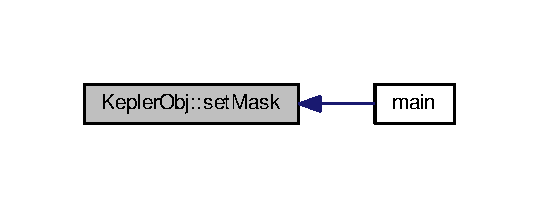
\includegraphics[width=258pt]{class_kepler_obj_a0712485c7f8f87047dff986c06bca53e_icgraph}
\end{center}
\end{figure}


\hypertarget{class_kepler_obj_a00f426d160b0674bfe52d2f36014e465}{\index{Kepler\-Obj@{Kepler\-Obj}!set\-Max\-Evals\-C\-S@{set\-Max\-Evals\-C\-S}}
\index{set\-Max\-Evals\-C\-S@{set\-Max\-Evals\-C\-S}!KeplerObj@{Kepler\-Obj}}
\subsubsection[{set\-Max\-Evals\-C\-S}]{\setlength{\rightskip}{0pt plus 5cm}void Kepler\-Obj\-::set\-Max\-Evals\-C\-S (
\begin{DoxyParamCaption}
{}
\end{DoxyParamCaption}
)}}\label{class_kepler_obj_a00f426d160b0674bfe52d2f36014e465}


Definition at line 178 of file Kepler.\-cpp.

\hypertarget{class_kepler_obj_a43d6d7205c8a92397558a97217511b62}{\index{Kepler\-Obj@{Kepler\-Obj}!set\-Max\-Evals\-S\-I@{set\-Max\-Evals\-S\-I}}
\index{set\-Max\-Evals\-S\-I@{set\-Max\-Evals\-S\-I}!KeplerObj@{Kepler\-Obj}}
\subsubsection[{set\-Max\-Evals\-S\-I}]{\setlength{\rightskip}{0pt plus 5cm}void Kepler\-Obj\-::set\-Max\-Evals\-S\-I (
\begin{DoxyParamCaption}
\item[{int}]{max\-Evals\-S\-I}
\end{DoxyParamCaption}
)}}\label{class_kepler_obj_a43d6d7205c8a92397558a97217511b62}


Definition at line 130 of file Kepler.\-cpp.

\hypertarget{class_kepler_obj_ab6eaf04d2a806c718a41c38a44af6190}{\index{Kepler\-Obj@{Kepler\-Obj}!set\-Max\-Evals\-S\-I\-I@{set\-Max\-Evals\-S\-I\-I}}
\index{set\-Max\-Evals\-S\-I\-I@{set\-Max\-Evals\-S\-I\-I}!KeplerObj@{Kepler\-Obj}}
\subsubsection[{set\-Max\-Evals\-S\-I\-I}]{\setlength{\rightskip}{0pt plus 5cm}void Kepler\-Obj\-::set\-Max\-Evals\-S\-I\-I (
\begin{DoxyParamCaption}
\item[{int}]{max\-Evals\-S\-I\-I}
\end{DoxyParamCaption}
)}}\label{class_kepler_obj_ab6eaf04d2a806c718a41c38a44af6190}


Definition at line 154 of file Kepler.\-cpp.

\hypertarget{class_kepler_obj_a94b23d5f4fe9142053e2c0a8d5a7eab4}{\index{Kepler\-Obj@{Kepler\-Obj}!set\-Num\-Chi\-Sq@{set\-Num\-Chi\-Sq}}
\index{set\-Num\-Chi\-Sq@{set\-Num\-Chi\-Sq}!KeplerObj@{Kepler\-Obj}}
\subsubsection[{set\-Num\-Chi\-Sq}]{\setlength{\rightskip}{0pt plus 5cm}void Kepler\-Obj\-::set\-Num\-Chi\-Sq (
\begin{DoxyParamCaption}
\item[{int}]{num\-Chi\-Sq}
\end{DoxyParamCaption}
)}}\label{class_kepler_obj_a94b23d5f4fe9142053e2c0a8d5a7eab4}


Definition at line 190 of file Kepler.\-cpp.

\hypertarget{class_kepler_obj_afaefc71cee5ab1f7fed60366910b77d2}{\index{Kepler\-Obj@{Kepler\-Obj}!set\-Num\-Seeds@{set\-Num\-Seeds}}
\index{set\-Num\-Seeds@{set\-Num\-Seeds}!KeplerObj@{Kepler\-Obj}}
\subsubsection[{set\-Num\-Seeds}]{\setlength{\rightskip}{0pt plus 5cm}void Kepler\-Obj\-::set\-Num\-Seeds (
\begin{DoxyParamCaption}
\item[{int}]{num\-Seeds}
\end{DoxyParamCaption}
)}}\label{class_kepler_obj_afaefc71cee5ab1f7fed60366910b77d2}


Definition at line 198 of file Kepler.\-cpp.

\hypertarget{class_kepler_obj_a78ddbc7c63e7d698e968a65d04ed5ae1}{\index{Kepler\-Obj@{Kepler\-Obj}!set\-Num\-Sims\-C\-S@{set\-Num\-Sims\-C\-S}}
\index{set\-Num\-Sims\-C\-S@{set\-Num\-Sims\-C\-S}!KeplerObj@{Kepler\-Obj}}
\subsubsection[{set\-Num\-Sims\-C\-S}]{\setlength{\rightskip}{0pt plus 5cm}void Kepler\-Obj\-::set\-Num\-Sims\-C\-S (
\begin{DoxyParamCaption}
\item[{int}]{num\-Sims\-C\-S}
\end{DoxyParamCaption}
)}}\label{class_kepler_obj_a78ddbc7c63e7d698e968a65d04ed5ae1}


Definition at line 174 of file Kepler.\-cpp.

\hypertarget{class_kepler_obj_ace628ec6c767aff9168497ec63984ccc}{\index{Kepler\-Obj@{Kepler\-Obj}!set\-Num\-Sims\-S\-I@{set\-Num\-Sims\-S\-I}}
\index{set\-Num\-Sims\-S\-I@{set\-Num\-Sims\-S\-I}!KeplerObj@{Kepler\-Obj}}
\subsubsection[{set\-Num\-Sims\-S\-I}]{\setlength{\rightskip}{0pt plus 5cm}void Kepler\-Obj\-::set\-Num\-Sims\-S\-I (
\begin{DoxyParamCaption}
\item[{int}]{num\-Sims\-S\-I}
\end{DoxyParamCaption}
)}}\label{class_kepler_obj_ace628ec6c767aff9168497ec63984ccc}


Definition at line 126 of file Kepler.\-cpp.

\hypertarget{class_kepler_obj_a762cbe9392ac57bcb4fa64858826e1f1}{\index{Kepler\-Obj@{Kepler\-Obj}!set\-Num\-Sims\-S\-I\-I@{set\-Num\-Sims\-S\-I\-I}}
\index{set\-Num\-Sims\-S\-I\-I@{set\-Num\-Sims\-S\-I\-I}!KeplerObj@{Kepler\-Obj}}
\subsubsection[{set\-Num\-Sims\-S\-I\-I}]{\setlength{\rightskip}{0pt plus 5cm}void Kepler\-Obj\-::set\-Num\-Sims\-S\-I\-I (
\begin{DoxyParamCaption}
\item[{int}]{num\-Sims\-S\-I\-I}
\end{DoxyParamCaption}
)}}\label{class_kepler_obj_a762cbe9392ac57bcb4fa64858826e1f1}


Definition at line 150 of file Kepler.\-cpp.

\hypertarget{class_kepler_obj_af7e062113cc6222956d892733b36142f}{\index{Kepler\-Obj@{Kepler\-Obj}!set\-Order@{set\-Order}}
\index{set\-Order@{set\-Order}!KeplerObj@{Kepler\-Obj}}
\subsubsection[{set\-Order}]{\setlength{\rightskip}{0pt plus 5cm}void Kepler\-Obj\-::set\-Order (
\begin{DoxyParamCaption}
\item[{int}]{ord}
\end{DoxyParamCaption}
)}}\label{class_kepler_obj_af7e062113cc6222956d892733b36142f}


Definition at line 78 of file Kepler.\-cpp.

\hypertarget{class_kepler_obj_a8cf9e305908521eaf390f5dd96fe9b4a}{\index{Kepler\-Obj@{Kepler\-Obj}!set\-Over\-Sample\-Factor@{set\-Over\-Sample\-Factor}}
\index{set\-Over\-Sample\-Factor@{set\-Over\-Sample\-Factor}!KeplerObj@{Kepler\-Obj}}
\subsubsection[{set\-Over\-Sample\-Factor}]{\setlength{\rightskip}{0pt plus 5cm}void Kepler\-Obj\-::set\-Over\-Sample\-Factor (
\begin{DoxyParamCaption}
\item[{int}]{over\-Sample\-Factor}
\end{DoxyParamCaption}
)}}\label{class_kepler_obj_a8cf9e305908521eaf390f5dd96fe9b4a}


Definition at line 94 of file Kepler.\-cpp.

\hypertarget{class_kepler_obj_a18ece34d36959a5eb0c75c34bdeea2ae}{\index{Kepler\-Obj@{Kepler\-Obj}!set\-Properties@{set\-Properties}}
\index{set\-Properties@{set\-Properties}!KeplerObj@{Kepler\-Obj}}
\subsubsection[{set\-Properties}]{\setlength{\rightskip}{0pt plus 5cm}void Kepler\-Obj\-::set\-Properties (
\begin{DoxyParamCaption}
\item[{const tuple$<$ vector$<$ array$<$ int, 2 $>$$>$, vector$<$ array$<$ double, 5 $>$$>$$>$ \&}]{data\-Array}
\end{DoxyParamCaption}
)}}\label{class_kepler_obj_a18ece34d36959a5eb0c75c34bdeea2ae}


Definition at line 747 of file Kepler.\-cpp.



Here is the caller graph for this function\-:\nopagebreak
\begin{figure}[H]
\begin{center}
\leavevmode
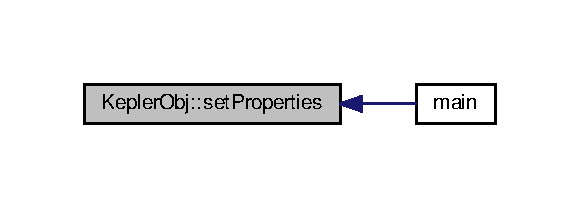
\includegraphics[width=278pt]{class_kepler_obj_a18ece34d36959a5eb0c75c34bdeea2ae_icgraph}
\end{center}
\end{figure}


\hypertarget{class_kepler_obj_afcd5f85bcd1f39d590d70e0dcdc1ee08}{\index{Kepler\-Obj@{Kepler\-Obj}!set\-Stage@{set\-Stage}}
\index{set\-Stage@{set\-Stage}!KeplerObj@{Kepler\-Obj}}
\subsubsection[{set\-Stage}]{\setlength{\rightskip}{0pt plus 5cm}void Kepler\-Obj\-::set\-Stage (
\begin{DoxyParamCaption}
\item[{int}]{stage}
\end{DoxyParamCaption}
)}}\label{class_kepler_obj_afcd5f85bcd1f39d590d70e0dcdc1ee08}


Definition at line 118 of file Kepler.\-cpp.



The documentation for this class was generated from the following files\-:\begin{DoxyCompactItemize}
\item 
/home/vish/code/trunk/cpp/libcarma/include/\hyperlink{_kepler_8hpp}{Kepler.\-hpp}\item 
/home/vish/code/trunk/cpp/libcarma/src/\hyperlink{_kepler_8cpp}{Kepler.\-cpp}\end{DoxyCompactItemize}

\hypertarget{struct_ln_like_args}{\section{Ln\-Like\-Args Struct Reference}
\label{struct_ln_like_args}\index{Ln\-Like\-Args@{Ln\-Like\-Args}}
}


{\ttfamily \#include $<$C\-A\-R\-M\-A.\-hpp$>$}



Collaboration diagram for Ln\-Like\-Args\-:\nopagebreak
\begin{figure}[H]
\begin{center}
\leavevmode
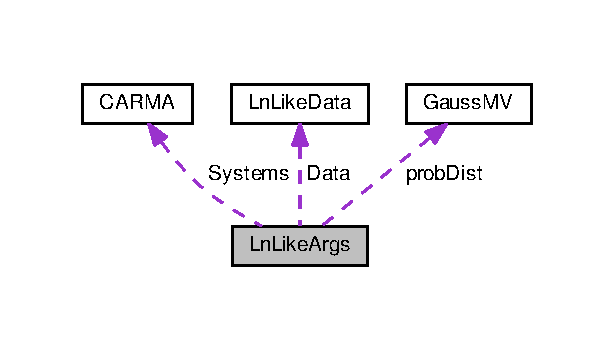
\includegraphics[width=294pt]{struct_ln_like_args__coll__graph}
\end{center}
\end{figure}
\subsection*{Public Attributes}
\begin{DoxyCompactItemize}
\item 
int \hyperlink{struct_ln_like_args_ad84da20749d9935f6a5a04b5c56d729a}{num\-Threads}
\item 
\hyperlink{class_c_a_r_m_a}{C\-A\-R\-M\-A} $\ast$ \hyperlink{struct_ln_like_args_af605bb6dcb409ad41dfc1a00c1e12c3f}{Systems}
\item 
\hyperlink{struct_ln_like_data}{Ln\-Like\-Data} \hyperlink{struct_ln_like_args_aa9a0a2c4945292f8429e4f0738db611b}{Data}
\item 
int \hyperlink{struct_ln_like_args_a14cedd7e2fed9d152ce3de6383567dad}{num\-Pts}
\item 
double $\ast$ \hyperlink{struct_ln_like_args_a49e48f13e6203cf7f629d3485416874f}{y}
\item 
\hyperlink{struct_gauss_m_v}{Gauss\-M\-V} \hyperlink{struct_ln_like_args_ad8d1ee1e21bab664c116720df98cf287}{prob\-Dist}
\end{DoxyCompactItemize}


\subsection{Detailed Description}


Definition at line 113 of file C\-A\-R\-M\-A.\-hpp.



\subsection{Member Data Documentation}
\hypertarget{struct_ln_like_args_aa9a0a2c4945292f8429e4f0738db611b}{\index{Ln\-Like\-Args@{Ln\-Like\-Args}!Data@{Data}}
\index{Data@{Data}!LnLikeArgs@{Ln\-Like\-Args}}
\subsubsection[{Data}]{\setlength{\rightskip}{0pt plus 5cm}{\bf Ln\-Like\-Data} Ln\-Like\-Args\-::\-Data}}\label{struct_ln_like_args_aa9a0a2c4945292f8429e4f0738db611b}


Definition at line 116 of file C\-A\-R\-M\-A.\-hpp.

\hypertarget{struct_ln_like_args_a14cedd7e2fed9d152ce3de6383567dad}{\index{Ln\-Like\-Args@{Ln\-Like\-Args}!num\-Pts@{num\-Pts}}
\index{num\-Pts@{num\-Pts}!LnLikeArgs@{Ln\-Like\-Args}}
\subsubsection[{num\-Pts}]{\setlength{\rightskip}{0pt plus 5cm}int Ln\-Like\-Args\-::num\-Pts}}\label{struct_ln_like_args_a14cedd7e2fed9d152ce3de6383567dad}


Definition at line 16 of file Gauss\-M\-V.\-hpp.

\hypertarget{struct_ln_like_args_ad84da20749d9935f6a5a04b5c56d729a}{\index{Ln\-Like\-Args@{Ln\-Like\-Args}!num\-Threads@{num\-Threads}}
\index{num\-Threads@{num\-Threads}!LnLikeArgs@{Ln\-Like\-Args}}
\subsubsection[{num\-Threads}]{\setlength{\rightskip}{0pt plus 5cm}int Ln\-Like\-Args\-::num\-Threads}}\label{struct_ln_like_args_ad84da20749d9935f6a5a04b5c56d729a}


Definition at line 114 of file C\-A\-R\-M\-A.\-hpp.

\hypertarget{struct_ln_like_args_ad8d1ee1e21bab664c116720df98cf287}{\index{Ln\-Like\-Args@{Ln\-Like\-Args}!prob\-Dist@{prob\-Dist}}
\index{prob\-Dist@{prob\-Dist}!LnLikeArgs@{Ln\-Like\-Args}}
\subsubsection[{prob\-Dist}]{\setlength{\rightskip}{0pt plus 5cm}{\bf Gauss\-M\-V} Ln\-Like\-Args\-::prob\-Dist}}\label{struct_ln_like_args_ad8d1ee1e21bab664c116720df98cf287}


Definition at line 18 of file Gauss\-M\-V.\-hpp.

\hypertarget{struct_ln_like_args_af605bb6dcb409ad41dfc1a00c1e12c3f}{\index{Ln\-Like\-Args@{Ln\-Like\-Args}!Systems@{Systems}}
\index{Systems@{Systems}!LnLikeArgs@{Ln\-Like\-Args}}
\subsubsection[{Systems}]{\setlength{\rightskip}{0pt plus 5cm}{\bf C\-A\-R\-M\-A}$\ast$ Ln\-Like\-Args\-::\-Systems}}\label{struct_ln_like_args_af605bb6dcb409ad41dfc1a00c1e12c3f}


Definition at line 115 of file C\-A\-R\-M\-A.\-hpp.

\hypertarget{struct_ln_like_args_a49e48f13e6203cf7f629d3485416874f}{\index{Ln\-Like\-Args@{Ln\-Like\-Args}!y@{y}}
\index{y@{y}!LnLikeArgs@{Ln\-Like\-Args}}
\subsubsection[{y}]{\setlength{\rightskip}{0pt plus 5cm}double$\ast$ Ln\-Like\-Args\-::y}}\label{struct_ln_like_args_a49e48f13e6203cf7f629d3485416874f}


Definition at line 17 of file Gauss\-M\-V.\-hpp.



The documentation for this struct was generated from the following files\-:\begin{DoxyCompactItemize}
\item 
/home/vish/code/trunk/cpp/libcarma/include/\hyperlink{_c_a_r_m_a_8hpp}{C\-A\-R\-M\-A.\-hpp}\item 
/home/vish/code/trunk/cpp/libcarma/include/\hyperlink{_gauss_m_v_8hpp}{Gauss\-M\-V.\-hpp}\end{DoxyCompactItemize}

\hypertarget{struct_ln_like_data}{\section{Ln\-Like\-Data Struct Reference}
\label{struct_ln_like_data}\index{Ln\-Like\-Data@{Ln\-Like\-Data}}
}


{\ttfamily \#include $<$C\-A\-R\-M\-A.\-hpp$>$}

\subsection*{Public Attributes}
\begin{DoxyCompactItemize}
\item 
int \hyperlink{struct_ln_like_data_a825ffbe1d96bd9f1c913ed95c83fd8de}{num\-Cadences}
\item 
bool \hyperlink{struct_ln_like_data_af49dc41383840c47d9e03c154c510912}{I\-R}
\item 
double \hyperlink{struct_ln_like_data_a0fcbb2527d414cc2b0fe576a7a61f45c}{tol\-I\-R}
\item 
double \hyperlink{struct_ln_like_data_acbb8573027fb54b1d207c126a64c49c9}{t\-\_\-incr}
\item 
double \hyperlink{struct_ln_like_data_a883ba357c5e5a7eff7fb9a25f130a0e7}{frac\-Intrinsic\-Var}
\item 
double \hyperlink{struct_ln_like_data_a9d90bcfebe1eec966719b8c0febb7dc7}{frac\-Noise\-To\-Signal}
\item 
double \hyperlink{struct_ln_like_data_ae30e91660af267721f78434f5e771293}{max\-Sigma}
\item 
double \hyperlink{struct_ln_like_data_a429a07a037a45e99a52c0c9e6193b23d}{min\-Timescale}
\item 
double \hyperlink{struct_ln_like_data_ab1c1eb4d8e84c78b1b76849adfd0aeb8}{max\-Timescale}
\item 
double $\ast$ \hyperlink{struct_ln_like_data_a5b1bf48c4b998b85df9c381974e65f93}{t}
\item 
double $\ast$ \hyperlink{struct_ln_like_data_afd71e6e5c9f90880038586d6f4e705fe}{x}
\item 
double $\ast$ \hyperlink{struct_ln_like_data_ac75cc1e68fffac23d841e09f927a0a53}{y}
\item 
double $\ast$ \hyperlink{struct_ln_like_data_a54330ef049f623a902d04f58e5aee208}{yerr}
\item 
double $\ast$ \hyperlink{struct_ln_like_data_a51c6e3bd71666d529910318735f0df21}{mask}
\end{DoxyCompactItemize}


\subsection{Detailed Description}


Definition at line 21 of file C\-A\-R\-M\-A.\-hpp.



\subsection{Member Data Documentation}
\hypertarget{struct_ln_like_data_a883ba357c5e5a7eff7fb9a25f130a0e7}{\index{Ln\-Like\-Data@{Ln\-Like\-Data}!frac\-Intrinsic\-Var@{frac\-Intrinsic\-Var}}
\index{frac\-Intrinsic\-Var@{frac\-Intrinsic\-Var}!LnLikeData@{Ln\-Like\-Data}}
\subsubsection[{frac\-Intrinsic\-Var}]{\setlength{\rightskip}{0pt plus 5cm}double Ln\-Like\-Data\-::frac\-Intrinsic\-Var}}\label{struct_ln_like_data_a883ba357c5e5a7eff7fb9a25f130a0e7}


Definition at line 26 of file C\-A\-R\-M\-A.\-hpp.

\hypertarget{struct_ln_like_data_a9d90bcfebe1eec966719b8c0febb7dc7}{\index{Ln\-Like\-Data@{Ln\-Like\-Data}!frac\-Noise\-To\-Signal@{frac\-Noise\-To\-Signal}}
\index{frac\-Noise\-To\-Signal@{frac\-Noise\-To\-Signal}!LnLikeData@{Ln\-Like\-Data}}
\subsubsection[{frac\-Noise\-To\-Signal}]{\setlength{\rightskip}{0pt plus 5cm}double Ln\-Like\-Data\-::frac\-Noise\-To\-Signal}}\label{struct_ln_like_data_a9d90bcfebe1eec966719b8c0febb7dc7}


Definition at line 27 of file C\-A\-R\-M\-A.\-hpp.

\hypertarget{struct_ln_like_data_af49dc41383840c47d9e03c154c510912}{\index{Ln\-Like\-Data@{Ln\-Like\-Data}!I\-R@{I\-R}}
\index{I\-R@{I\-R}!LnLikeData@{Ln\-Like\-Data}}
\subsubsection[{I\-R}]{\setlength{\rightskip}{0pt plus 5cm}bool Ln\-Like\-Data\-::\-I\-R}}\label{struct_ln_like_data_af49dc41383840c47d9e03c154c510912}


Definition at line 23 of file C\-A\-R\-M\-A.\-hpp.

\hypertarget{struct_ln_like_data_a51c6e3bd71666d529910318735f0df21}{\index{Ln\-Like\-Data@{Ln\-Like\-Data}!mask@{mask}}
\index{mask@{mask}!LnLikeData@{Ln\-Like\-Data}}
\subsubsection[{mask}]{\setlength{\rightskip}{0pt plus 5cm}double$\ast$ Ln\-Like\-Data\-::mask}}\label{struct_ln_like_data_a51c6e3bd71666d529910318735f0df21}


Definition at line 35 of file C\-A\-R\-M\-A.\-hpp.

\hypertarget{struct_ln_like_data_ae30e91660af267721f78434f5e771293}{\index{Ln\-Like\-Data@{Ln\-Like\-Data}!max\-Sigma@{max\-Sigma}}
\index{max\-Sigma@{max\-Sigma}!LnLikeData@{Ln\-Like\-Data}}
\subsubsection[{max\-Sigma}]{\setlength{\rightskip}{0pt plus 5cm}double Ln\-Like\-Data\-::max\-Sigma}}\label{struct_ln_like_data_ae30e91660af267721f78434f5e771293}


Definition at line 28 of file C\-A\-R\-M\-A.\-hpp.

\hypertarget{struct_ln_like_data_ab1c1eb4d8e84c78b1b76849adfd0aeb8}{\index{Ln\-Like\-Data@{Ln\-Like\-Data}!max\-Timescale@{max\-Timescale}}
\index{max\-Timescale@{max\-Timescale}!LnLikeData@{Ln\-Like\-Data}}
\subsubsection[{max\-Timescale}]{\setlength{\rightskip}{0pt plus 5cm}double Ln\-Like\-Data\-::max\-Timescale}}\label{struct_ln_like_data_ab1c1eb4d8e84c78b1b76849adfd0aeb8}


Definition at line 30 of file C\-A\-R\-M\-A.\-hpp.

\hypertarget{struct_ln_like_data_a429a07a037a45e99a52c0c9e6193b23d}{\index{Ln\-Like\-Data@{Ln\-Like\-Data}!min\-Timescale@{min\-Timescale}}
\index{min\-Timescale@{min\-Timescale}!LnLikeData@{Ln\-Like\-Data}}
\subsubsection[{min\-Timescale}]{\setlength{\rightskip}{0pt plus 5cm}double Ln\-Like\-Data\-::min\-Timescale}}\label{struct_ln_like_data_a429a07a037a45e99a52c0c9e6193b23d}


Definition at line 29 of file C\-A\-R\-M\-A.\-hpp.

\hypertarget{struct_ln_like_data_a825ffbe1d96bd9f1c913ed95c83fd8de}{\index{Ln\-Like\-Data@{Ln\-Like\-Data}!num\-Cadences@{num\-Cadences}}
\index{num\-Cadences@{num\-Cadences}!LnLikeData@{Ln\-Like\-Data}}
\subsubsection[{num\-Cadences}]{\setlength{\rightskip}{0pt plus 5cm}int Ln\-Like\-Data\-::num\-Cadences}}\label{struct_ln_like_data_a825ffbe1d96bd9f1c913ed95c83fd8de}


Definition at line 22 of file C\-A\-R\-M\-A.\-hpp.

\hypertarget{struct_ln_like_data_a5b1bf48c4b998b85df9c381974e65f93}{\index{Ln\-Like\-Data@{Ln\-Like\-Data}!t@{t}}
\index{t@{t}!LnLikeData@{Ln\-Like\-Data}}
\subsubsection[{t}]{\setlength{\rightskip}{0pt plus 5cm}double$\ast$ Ln\-Like\-Data\-::t}}\label{struct_ln_like_data_a5b1bf48c4b998b85df9c381974e65f93}


Definition at line 31 of file C\-A\-R\-M\-A.\-hpp.

\hypertarget{struct_ln_like_data_acbb8573027fb54b1d207c126a64c49c9}{\index{Ln\-Like\-Data@{Ln\-Like\-Data}!t\-\_\-incr@{t\-\_\-incr}}
\index{t\-\_\-incr@{t\-\_\-incr}!LnLikeData@{Ln\-Like\-Data}}
\subsubsection[{t\-\_\-incr}]{\setlength{\rightskip}{0pt plus 5cm}double Ln\-Like\-Data\-::t\-\_\-incr}}\label{struct_ln_like_data_acbb8573027fb54b1d207c126a64c49c9}


Definition at line 25 of file C\-A\-R\-M\-A.\-hpp.

\hypertarget{struct_ln_like_data_a0fcbb2527d414cc2b0fe576a7a61f45c}{\index{Ln\-Like\-Data@{Ln\-Like\-Data}!tol\-I\-R@{tol\-I\-R}}
\index{tol\-I\-R@{tol\-I\-R}!LnLikeData@{Ln\-Like\-Data}}
\subsubsection[{tol\-I\-R}]{\setlength{\rightskip}{0pt plus 5cm}double Ln\-Like\-Data\-::tol\-I\-R}}\label{struct_ln_like_data_a0fcbb2527d414cc2b0fe576a7a61f45c}


Definition at line 24 of file C\-A\-R\-M\-A.\-hpp.

\hypertarget{struct_ln_like_data_afd71e6e5c9f90880038586d6f4e705fe}{\index{Ln\-Like\-Data@{Ln\-Like\-Data}!x@{x}}
\index{x@{x}!LnLikeData@{Ln\-Like\-Data}}
\subsubsection[{x}]{\setlength{\rightskip}{0pt plus 5cm}double$\ast$ Ln\-Like\-Data\-::x}}\label{struct_ln_like_data_afd71e6e5c9f90880038586d6f4e705fe}


Definition at line 32 of file C\-A\-R\-M\-A.\-hpp.

\hypertarget{struct_ln_like_data_ac75cc1e68fffac23d841e09f927a0a53}{\index{Ln\-Like\-Data@{Ln\-Like\-Data}!y@{y}}
\index{y@{y}!LnLikeData@{Ln\-Like\-Data}}
\subsubsection[{y}]{\setlength{\rightskip}{0pt plus 5cm}double$\ast$ Ln\-Like\-Data\-::y}}\label{struct_ln_like_data_ac75cc1e68fffac23d841e09f927a0a53}


Definition at line 33 of file C\-A\-R\-M\-A.\-hpp.

\hypertarget{struct_ln_like_data_a54330ef049f623a902d04f58e5aee208}{\index{Ln\-Like\-Data@{Ln\-Like\-Data}!yerr@{yerr}}
\index{yerr@{yerr}!LnLikeData@{Ln\-Like\-Data}}
\subsubsection[{yerr}]{\setlength{\rightskip}{0pt plus 5cm}double$\ast$ Ln\-Like\-Data\-::yerr}}\label{struct_ln_like_data_a54330ef049f623a902d04f58e5aee208}


Definition at line 34 of file C\-A\-R\-M\-A.\-hpp.



The documentation for this struct was generated from the following file\-:\begin{DoxyCompactItemize}
\item 
/home/vish/code/trunk/cpp/libcarma/cython/include/\hyperlink{_c_a_r_m_a_8hpp}{C\-A\-R\-M\-A.\-hpp}\end{DoxyCompactItemize}

\hypertarget{class_obj}{\section{Obj Class Reference}
\label{class_obj}\index{Obj@{Obj}}
}


{\ttfamily \#include $<$Obj.\-hpp$>$}



Inheritance diagram for Obj\-:\nopagebreak
\begin{figure}[H]
\begin{center}
\leavevmode
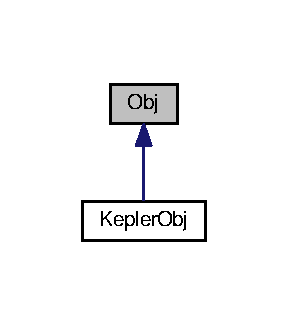
\includegraphics[width=138pt]{class_obj__inherit__graph}
\end{center}
\end{figure}


Collaboration diagram for Obj\-:\nopagebreak
\begin{figure}[H]
\begin{center}
\leavevmode
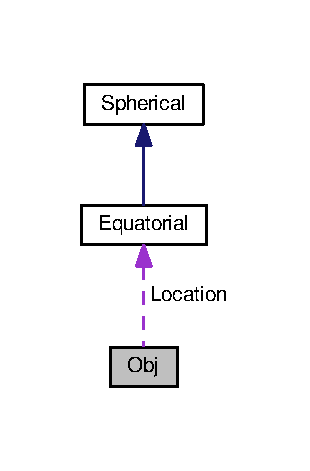
\includegraphics[width=149pt]{class_obj__coll__graph}
\end{center}
\end{figure}
\subsection*{Public Member Functions}
\begin{DoxyCompactItemize}
\item 
\hyperlink{class_obj_ae6d85a21719815c7bbb9cd68d609e0a0}{Obj} ()
\item 
\hyperlink{class_obj_a36ce6f3ebbb04e1eaa616a68adca59fe}{Obj} (array$<$ double, 3 $>$ pos)
\item 
\hyperlink{class_obj_a376349e92c61e68b131fe662cb781a16}{Obj} (\hyperlink{class_equatorial}{Equatorial} loc)
\item 
\hyperlink{class_obj_a4fdf8a5a6959362fc757c90d5b5edcd0}{Obj} (string identifier, array$<$ double, 3 $>$ pos)
\item 
\hyperlink{class_obj_a49b473cf45363f170001c80ac66ace62}{Obj} (string identifier, \hyperlink{class_equatorial}{Equatorial} loc)
\item 
\hyperlink{class_obj_a106e577728a05a08d41ada3c286bb613}{Obj} (vector$<$ string $>$ identifier, array$<$ double, 3 $>$ pos)
\item 
\hyperlink{class_obj_adaf14990af8049cccb1314e425b7615a}{Obj} (vector$<$ string $>$ identifier, \hyperlink{class_equatorial}{Equatorial} loc)
\item 
virtual \hyperlink{class_obj_a1331b88810f8f346b820cb855955feea}{$\sim$\-Obj} ()=default
\item 
string \hyperlink{class_obj_ab8db1493558965a3d895a486d641716e}{get\-Identifier} (int number)
\item 
vector$<$ string $>$ \hyperlink{class_obj_a2eeea0eace0600a188146e0021503cc7}{get\-Identifier} ()
\item 
void \hyperlink{class_obj_afb9cdab9ce6d9b5ae6942465b91f14d1}{add\-Identifier} (string identifier)
\item 
void \hyperlink{class_obj_af54187bd0affc6d46fdb85af1d35de8a}{add\-Identifier} (vector$<$ string $>$ identifier)
\item 
\hyperlink{class_equatorial}{Equatorial} \hyperlink{class_obj_a37de1c5bfaa5b641bf6f093a809cc8d0}{get\-Location} ()
\item 
double \hyperlink{class_obj_ab4a4130741f5641d97ca33f4468dc9a3}{radial\-Comoving\-Distance} (const \hyperlink{class_universe}{Universe} \&u)
\item 
double \hyperlink{class_obj_a75e3651dda7a1262c4f7c6ff431bb9c8}{transverse\-Comoving\-Distance} (const \hyperlink{class_universe}{Universe} \&u)
\item 
double \hyperlink{class_obj_a4e0add44503b0efdc90046f8eabd1d6d}{angular\-Diameter\-Distance} (const \hyperlink{class_universe}{Universe} \&u)
\item 
double \hyperlink{class_obj_ae168d94748733f995bdfeb8440d332a3}{luminosity\-Distance} (const \hyperlink{class_universe}{Universe} \&u)
\item 
double \hyperlink{class_obj_a6107516e388eb66505d684f977dceac0}{look\-Back\-Time} (const \hyperlink{class_universe}{Universe} \&u)
\end{DoxyCompactItemize}
\subsection*{Protected Attributes}
\begin{DoxyCompactItemize}
\item 
vector$<$ string $>$ \hyperlink{class_obj_a355b268a6191d208fe8783bc6b259080}{Identifier}
\item 
\hyperlink{class_equatorial}{Equatorial} \hyperlink{class_obj_a15ef308c438130b6a99dd99c40bc8ade}{Location}
\end{DoxyCompactItemize}


\subsection{Detailed Description}


Definition at line 9 of file Obj.\-hpp.



\subsection{Constructor \& Destructor Documentation}
\hypertarget{class_obj_ae6d85a21719815c7bbb9cd68d609e0a0}{\index{Obj@{Obj}!Obj@{Obj}}
\index{Obj@{Obj}!Obj@{Obj}}
\subsubsection[{Obj}]{\setlength{\rightskip}{0pt plus 5cm}Obj\-::\-Obj (
\begin{DoxyParamCaption}
{}
\end{DoxyParamCaption}
)}}\label{class_obj_ae6d85a21719815c7bbb9cd68d609e0a0}


Definition at line 10 of file Obj.\-cpp.

\hypertarget{class_obj_a36ce6f3ebbb04e1eaa616a68adca59fe}{\index{Obj@{Obj}!Obj@{Obj}}
\index{Obj@{Obj}!Obj@{Obj}}
\subsubsection[{Obj}]{\setlength{\rightskip}{0pt plus 5cm}Obj\-::\-Obj (
\begin{DoxyParamCaption}
\item[{array$<$ double, 3 $>$}]{pos}
\end{DoxyParamCaption}
)}}\label{class_obj_a36ce6f3ebbb04e1eaa616a68adca59fe}


Definition at line 17 of file Obj.\-cpp.

\hypertarget{class_obj_a376349e92c61e68b131fe662cb781a16}{\index{Obj@{Obj}!Obj@{Obj}}
\index{Obj@{Obj}!Obj@{Obj}}
\subsubsection[{Obj}]{\setlength{\rightskip}{0pt plus 5cm}Obj\-::\-Obj (
\begin{DoxyParamCaption}
\item[{{\bf Equatorial}}]{loc}
\end{DoxyParamCaption}
)}}\label{class_obj_a376349e92c61e68b131fe662cb781a16}


Definition at line 27 of file Obj.\-cpp.

\hypertarget{class_obj_a4fdf8a5a6959362fc757c90d5b5edcd0}{\index{Obj@{Obj}!Obj@{Obj}}
\index{Obj@{Obj}!Obj@{Obj}}
\subsubsection[{Obj}]{\setlength{\rightskip}{0pt plus 5cm}Obj\-::\-Obj (
\begin{DoxyParamCaption}
\item[{string}]{identifier, }
\item[{array$<$ double, 3 $>$}]{pos}
\end{DoxyParamCaption}
)}}\label{class_obj_a4fdf8a5a6959362fc757c90d5b5edcd0}


Definition at line 22 of file Obj.\-cpp.

\hypertarget{class_obj_a49b473cf45363f170001c80ac66ace62}{\index{Obj@{Obj}!Obj@{Obj}}
\index{Obj@{Obj}!Obj@{Obj}}
\subsubsection[{Obj}]{\setlength{\rightskip}{0pt plus 5cm}Obj\-::\-Obj (
\begin{DoxyParamCaption}
\item[{string}]{identifier, }
\item[{{\bf Equatorial}}]{loc}
\end{DoxyParamCaption}
)}}\label{class_obj_a49b473cf45363f170001c80ac66ace62}


Definition at line 32 of file Obj.\-cpp.

\hypertarget{class_obj_a106e577728a05a08d41ada3c286bb613}{\index{Obj@{Obj}!Obj@{Obj}}
\index{Obj@{Obj}!Obj@{Obj}}
\subsubsection[{Obj}]{\setlength{\rightskip}{0pt plus 5cm}Obj\-::\-Obj (
\begin{DoxyParamCaption}
\item[{vector$<$ string $>$}]{identifier, }
\item[{array$<$ double, 3 $>$}]{pos}
\end{DoxyParamCaption}
)}}\label{class_obj_a106e577728a05a08d41ada3c286bb613}


Definition at line 37 of file Obj.\-cpp.

\hypertarget{class_obj_adaf14990af8049cccb1314e425b7615a}{\index{Obj@{Obj}!Obj@{Obj}}
\index{Obj@{Obj}!Obj@{Obj}}
\subsubsection[{Obj}]{\setlength{\rightskip}{0pt plus 5cm}Obj\-::\-Obj (
\begin{DoxyParamCaption}
\item[{vector$<$ string $>$}]{identifier, }
\item[{{\bf Equatorial}}]{loc}
\end{DoxyParamCaption}
)}}\label{class_obj_adaf14990af8049cccb1314e425b7615a}


Definition at line 42 of file Obj.\-cpp.

\hypertarget{class_obj_a1331b88810f8f346b820cb855955feea}{\index{Obj@{Obj}!$\sim$\-Obj@{$\sim$\-Obj}}
\index{$\sim$\-Obj@{$\sim$\-Obj}!Obj@{Obj}}
\subsubsection[{$\sim$\-Obj}]{\setlength{\rightskip}{0pt plus 5cm}virtual Obj\-::$\sim$\-Obj (
\begin{DoxyParamCaption}
{}
\end{DoxyParamCaption}
)\hspace{0.3cm}{\ttfamily [virtual]}, {\ttfamily [default]}}}\label{class_obj_a1331b88810f8f346b820cb855955feea}


\subsection{Member Function Documentation}
\hypertarget{class_obj_afb9cdab9ce6d9b5ae6942465b91f14d1}{\index{Obj@{Obj}!add\-Identifier@{add\-Identifier}}
\index{add\-Identifier@{add\-Identifier}!Obj@{Obj}}
\subsubsection[{add\-Identifier}]{\setlength{\rightskip}{0pt plus 5cm}void Obj\-::add\-Identifier (
\begin{DoxyParamCaption}
\item[{string}]{identifier}
\end{DoxyParamCaption}
)}}\label{class_obj_afb9cdab9ce6d9b5ae6942465b91f14d1}


Definition at line 58 of file Obj.\-cpp.

\hypertarget{class_obj_af54187bd0affc6d46fdb85af1d35de8a}{\index{Obj@{Obj}!add\-Identifier@{add\-Identifier}}
\index{add\-Identifier@{add\-Identifier}!Obj@{Obj}}
\subsubsection[{add\-Identifier}]{\setlength{\rightskip}{0pt plus 5cm}void Obj\-::add\-Identifier (
\begin{DoxyParamCaption}
\item[{vector$<$ string $>$}]{identifier}
\end{DoxyParamCaption}
)}}\label{class_obj_af54187bd0affc6d46fdb85af1d35de8a}


Definition at line 62 of file Obj.\-cpp.

\hypertarget{class_obj_a4e0add44503b0efdc90046f8eabd1d6d}{\index{Obj@{Obj}!angular\-Diameter\-Distance@{angular\-Diameter\-Distance}}
\index{angular\-Diameter\-Distance@{angular\-Diameter\-Distance}!Obj@{Obj}}
\subsubsection[{angular\-Diameter\-Distance}]{\setlength{\rightskip}{0pt plus 5cm}double Obj\-::angular\-Diameter\-Distance (
\begin{DoxyParamCaption}
\item[{const {\bf Universe} \&}]{u}
\end{DoxyParamCaption}
)}}\label{class_obj_a4e0add44503b0efdc90046f8eabd1d6d}


Definition at line 80 of file Obj.\-cpp.

\hypertarget{class_obj_ab8db1493558965a3d895a486d641716e}{\index{Obj@{Obj}!get\-Identifier@{get\-Identifier}}
\index{get\-Identifier@{get\-Identifier}!Obj@{Obj}}
\subsubsection[{get\-Identifier}]{\setlength{\rightskip}{0pt plus 5cm}string Obj\-::get\-Identifier (
\begin{DoxyParamCaption}
\item[{int}]{number}
\end{DoxyParamCaption}
)}}\label{class_obj_ab8db1493558965a3d895a486d641716e}


Definition at line 47 of file Obj.\-cpp.

\hypertarget{class_obj_a2eeea0eace0600a188146e0021503cc7}{\index{Obj@{Obj}!get\-Identifier@{get\-Identifier}}
\index{get\-Identifier@{get\-Identifier}!Obj@{Obj}}
\subsubsection[{get\-Identifier}]{\setlength{\rightskip}{0pt plus 5cm}vector$<$ string $>$ Obj\-::get\-Identifier (
\begin{DoxyParamCaption}
{}
\end{DoxyParamCaption}
)}}\label{class_obj_a2eeea0eace0600a188146e0021503cc7}


Definition at line 54 of file Obj.\-cpp.

\hypertarget{class_obj_a37de1c5bfaa5b641bf6f093a809cc8d0}{\index{Obj@{Obj}!get\-Location@{get\-Location}}
\index{get\-Location@{get\-Location}!Obj@{Obj}}
\subsubsection[{get\-Location}]{\setlength{\rightskip}{0pt plus 5cm}{\bf Equatorial} Obj\-::get\-Location (
\begin{DoxyParamCaption}
{}
\end{DoxyParamCaption}
)}}\label{class_obj_a37de1c5bfaa5b641bf6f093a809cc8d0}


Definition at line 68 of file Obj.\-cpp.

\hypertarget{class_obj_a6107516e388eb66505d684f977dceac0}{\index{Obj@{Obj}!look\-Back\-Time@{look\-Back\-Time}}
\index{look\-Back\-Time@{look\-Back\-Time}!Obj@{Obj}}
\subsubsection[{look\-Back\-Time}]{\setlength{\rightskip}{0pt plus 5cm}double Obj\-::look\-Back\-Time (
\begin{DoxyParamCaption}
\item[{const {\bf Universe} \&}]{u}
\end{DoxyParamCaption}
)}}\label{class_obj_a6107516e388eb66505d684f977dceac0}


Definition at line 88 of file Obj.\-cpp.

\hypertarget{class_obj_ae168d94748733f995bdfeb8440d332a3}{\index{Obj@{Obj}!luminosity\-Distance@{luminosity\-Distance}}
\index{luminosity\-Distance@{luminosity\-Distance}!Obj@{Obj}}
\subsubsection[{luminosity\-Distance}]{\setlength{\rightskip}{0pt plus 5cm}double Obj\-::luminosity\-Distance (
\begin{DoxyParamCaption}
\item[{const {\bf Universe} \&}]{u}
\end{DoxyParamCaption}
)}}\label{class_obj_ae168d94748733f995bdfeb8440d332a3}


Definition at line 84 of file Obj.\-cpp.

\hypertarget{class_obj_ab4a4130741f5641d97ca33f4468dc9a3}{\index{Obj@{Obj}!radial\-Comoving\-Distance@{radial\-Comoving\-Distance}}
\index{radial\-Comoving\-Distance@{radial\-Comoving\-Distance}!Obj@{Obj}}
\subsubsection[{radial\-Comoving\-Distance}]{\setlength{\rightskip}{0pt plus 5cm}double Obj\-::radial\-Comoving\-Distance (
\begin{DoxyParamCaption}
\item[{const {\bf Universe} \&}]{u}
\end{DoxyParamCaption}
)}}\label{class_obj_ab4a4130741f5641d97ca33f4468dc9a3}


Definition at line 72 of file Obj.\-cpp.

\hypertarget{class_obj_a75e3651dda7a1262c4f7c6ff431bb9c8}{\index{Obj@{Obj}!transverse\-Comoving\-Distance@{transverse\-Comoving\-Distance}}
\index{transverse\-Comoving\-Distance@{transverse\-Comoving\-Distance}!Obj@{Obj}}
\subsubsection[{transverse\-Comoving\-Distance}]{\setlength{\rightskip}{0pt plus 5cm}double Obj\-::transverse\-Comoving\-Distance (
\begin{DoxyParamCaption}
\item[{const {\bf Universe} \&}]{u}
\end{DoxyParamCaption}
)}}\label{class_obj_a75e3651dda7a1262c4f7c6ff431bb9c8}


Definition at line 76 of file Obj.\-cpp.



\subsection{Member Data Documentation}
\hypertarget{class_obj_a355b268a6191d208fe8783bc6b259080}{\index{Obj@{Obj}!Identifier@{Identifier}}
\index{Identifier@{Identifier}!Obj@{Obj}}
\subsubsection[{Identifier}]{\setlength{\rightskip}{0pt plus 5cm}vector$<$string$>$ Obj\-::\-Identifier\hspace{0.3cm}{\ttfamily [protected]}}}\label{class_obj_a355b268a6191d208fe8783bc6b259080}


Definition at line 11 of file Obj.\-hpp.

\hypertarget{class_obj_a15ef308c438130b6a99dd99c40bc8ade}{\index{Obj@{Obj}!Location@{Location}}
\index{Location@{Location}!Obj@{Obj}}
\subsubsection[{Location}]{\setlength{\rightskip}{0pt plus 5cm}{\bf Equatorial} Obj\-::\-Location\hspace{0.3cm}{\ttfamily [protected]}}}\label{class_obj_a15ef308c438130b6a99dd99c40bc8ade}


Definition at line 12 of file Obj.\-hpp.



The documentation for this class was generated from the following files\-:\begin{DoxyCompactItemize}
\item 
/home/vish/code/trunk/cpp/libcarma/include/\hyperlink{_obj_8hpp}{Obj.\-hpp}\item 
/home/vish/code/trunk/cpp/libcarma/src/\hyperlink{_obj_8cpp}{Obj.\-cpp}\end{DoxyCompactItemize}

\hypertarget{class_spherical}{\section{Spherical Class Reference}
\label{class_spherical}\index{Spherical@{Spherical}}
}


{\ttfamily \#include $<$Spherical.\-hpp$>$}



Inheritance diagram for Spherical\-:\nopagebreak
\begin{figure}[H]
\begin{center}
\leavevmode
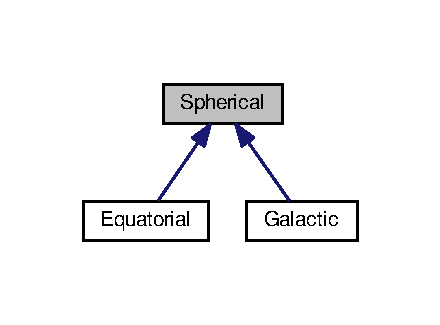
\includegraphics[width=211pt]{class_spherical__inherit__graph}
\end{center}
\end{figure}
\subsection*{Public Member Functions}
\begin{DoxyCompactItemize}
\item 
\hyperlink{class_spherical_ae043654d8006024f2c53aaa6ba35d05d}{Spherical} ()=default
\item 
\hyperlink{class_spherical_aed44cb28b5f4aaf1b98bfb949dddc495}{Spherical} (array$<$ double, 3 $>$ pos)
\item 
double \hyperlink{class_spherical_a6d4d86228d3fc54008206e75a2fa5f13}{get\-Red\-Shift} ()
\item 
double \hyperlink{class_spherical_acab04a7df5d746f275de748c3bae78ed}{radial\-Comoving\-Distance} (const \hyperlink{class_universe}{Universe} \&u)
\item 
double \hyperlink{class_spherical_a973fd2f86c54c2ca0c6adbdc3b869b41}{transverse\-Comoving\-Distance} (const \hyperlink{class_universe}{Universe} \&u)
\item 
double \hyperlink{class_spherical_aec39dd15b36585358eed8168d37b6455}{angular\-Diameter\-Distance} (const \hyperlink{class_universe}{Universe} \&u)
\item 
double \hyperlink{class_spherical_a66d8954554041cc005c3fc437bd5293e}{luminosity\-Distance} (const \hyperlink{class_universe}{Universe} \&u)
\item 
double \hyperlink{class_spherical_a2015656786c8277a9c419f9fa7526246}{look\-Back\-Time} (const \hyperlink{class_universe}{Universe} \&u)
\end{DoxyCompactItemize}
\subsection*{Protected Attributes}
\begin{DoxyCompactItemize}
\item 
array$<$ double, 3 $>$ \hyperlink{class_spherical_a5392e2db54d96ef3d687e007d06982fa}{Position}
\end{DoxyCompactItemize}
\subsection*{Friends}
\begin{DoxyCompactItemize}
\item 
class \hyperlink{class_spherical_a438b315afa8c872673a2dc740ac8243d}{Obj}
\item 
class \hyperlink{class_spherical_ab594011d9eb73ce33234ae0e11850252}{Kepler\-Obj}
\item 
bool \hyperlink{class_spherical_aff27ce80712096c80dcede74e1d23817}{operator==} (const \hyperlink{class_spherical}{Spherical} \&sph1, const \hyperlink{class_spherical}{Spherical} \&sph2)
\item 
bool \hyperlink{class_spherical_a58c3c65d834ad03dfa96936a815a78f0}{operator!=} (const \hyperlink{class_spherical}{Spherical} \&sph1, const \hyperlink{class_spherical}{Spherical} \&sph2)
\end{DoxyCompactItemize}


\subsection{Detailed Description}


Definition at line 17 of file Spherical.\-hpp.



\subsection{Constructor \& Destructor Documentation}
\hypertarget{class_spherical_ae043654d8006024f2c53aaa6ba35d05d}{\index{Spherical@{Spherical}!Spherical@{Spherical}}
\index{Spherical@{Spherical}!Spherical@{Spherical}}
\subsubsection[{Spherical}]{\setlength{\rightskip}{0pt plus 5cm}Spherical\-::\-Spherical (
\begin{DoxyParamCaption}
{}
\end{DoxyParamCaption}
)\hspace{0.3cm}{\ttfamily [default]}}}\label{class_spherical_ae043654d8006024f2c53aaa6ba35d05d}
\hypertarget{class_spherical_aed44cb28b5f4aaf1b98bfb949dddc495}{\index{Spherical@{Spherical}!Spherical@{Spherical}}
\index{Spherical@{Spherical}!Spherical@{Spherical}}
\subsubsection[{Spherical}]{\setlength{\rightskip}{0pt plus 5cm}Spherical\-::\-Spherical (
\begin{DoxyParamCaption}
\item[{array$<$ double, 3 $>$}]{pos}
\end{DoxyParamCaption}
)}}\label{class_spherical_aed44cb28b5f4aaf1b98bfb949dddc495}


Definition at line 12 of file Spherical.\-cpp.



\subsection{Member Function Documentation}
\hypertarget{class_spherical_aec39dd15b36585358eed8168d37b6455}{\index{Spherical@{Spherical}!angular\-Diameter\-Distance@{angular\-Diameter\-Distance}}
\index{angular\-Diameter\-Distance@{angular\-Diameter\-Distance}!Spherical@{Spherical}}
\subsubsection[{angular\-Diameter\-Distance}]{\setlength{\rightskip}{0pt plus 5cm}double Spherical\-::angular\-Diameter\-Distance (
\begin{DoxyParamCaption}
\item[{const {\bf Universe} \&}]{u}
\end{DoxyParamCaption}
)}}\label{class_spherical_aec39dd15b36585358eed8168d37b6455}


Definition at line 48 of file Spherical.\-cpp.

\hypertarget{class_spherical_a6d4d86228d3fc54008206e75a2fa5f13}{\index{Spherical@{Spherical}!get\-Red\-Shift@{get\-Red\-Shift}}
\index{get\-Red\-Shift@{get\-Red\-Shift}!Spherical@{Spherical}}
\subsubsection[{get\-Red\-Shift}]{\setlength{\rightskip}{0pt plus 5cm}double Spherical\-::get\-Red\-Shift (
\begin{DoxyParamCaption}
{}
\end{DoxyParamCaption}
)}}\label{class_spherical_a6d4d86228d3fc54008206e75a2fa5f13}


Definition at line 16 of file Spherical.\-cpp.

\hypertarget{class_spherical_a2015656786c8277a9c419f9fa7526246}{\index{Spherical@{Spherical}!look\-Back\-Time@{look\-Back\-Time}}
\index{look\-Back\-Time@{look\-Back\-Time}!Spherical@{Spherical}}
\subsubsection[{look\-Back\-Time}]{\setlength{\rightskip}{0pt plus 5cm}double Spherical\-::look\-Back\-Time (
\begin{DoxyParamCaption}
\item[{const {\bf Universe} \&}]{u}
\end{DoxyParamCaption}
)}}\label{class_spherical_a2015656786c8277a9c419f9fa7526246}


Definition at line 88 of file Spherical.\-cpp.

\hypertarget{class_spherical_a66d8954554041cc005c3fc437bd5293e}{\index{Spherical@{Spherical}!luminosity\-Distance@{luminosity\-Distance}}
\index{luminosity\-Distance@{luminosity\-Distance}!Spherical@{Spherical}}
\subsubsection[{luminosity\-Distance}]{\setlength{\rightskip}{0pt plus 5cm}double Spherical\-::luminosity\-Distance (
\begin{DoxyParamCaption}
\item[{const {\bf Universe} \&}]{u}
\end{DoxyParamCaption}
)}}\label{class_spherical_a66d8954554041cc005c3fc437bd5293e}


Definition at line 68 of file Spherical.\-cpp.

\hypertarget{class_spherical_acab04a7df5d746f275de748c3bae78ed}{\index{Spherical@{Spherical}!radial\-Comoving\-Distance@{radial\-Comoving\-Distance}}
\index{radial\-Comoving\-Distance@{radial\-Comoving\-Distance}!Spherical@{Spherical}}
\subsubsection[{radial\-Comoving\-Distance}]{\setlength{\rightskip}{0pt plus 5cm}double Spherical\-::radial\-Comoving\-Distance (
\begin{DoxyParamCaption}
\item[{const {\bf Universe} \&}]{u}
\end{DoxyParamCaption}
)}}\label{class_spherical_acab04a7df5d746f275de748c3bae78ed}


Definition at line 20 of file Spherical.\-cpp.

\hypertarget{class_spherical_a973fd2f86c54c2ca0c6adbdc3b869b41}{\index{Spherical@{Spherical}!transverse\-Comoving\-Distance@{transverse\-Comoving\-Distance}}
\index{transverse\-Comoving\-Distance@{transverse\-Comoving\-Distance}!Spherical@{Spherical}}
\subsubsection[{transverse\-Comoving\-Distance}]{\setlength{\rightskip}{0pt plus 5cm}double Spherical\-::transverse\-Comoving\-Distance (
\begin{DoxyParamCaption}
\item[{const {\bf Universe} \&}]{u}
\end{DoxyParamCaption}
)}}\label{class_spherical_a973fd2f86c54c2ca0c6adbdc3b869b41}


Definition at line 28 of file Spherical.\-cpp.



\subsection{Friends And Related Function Documentation}
\hypertarget{class_spherical_ab594011d9eb73ce33234ae0e11850252}{\index{Spherical@{Spherical}!Kepler\-Obj@{Kepler\-Obj}}
\index{Kepler\-Obj@{Kepler\-Obj}!Spherical@{Spherical}}
\subsubsection[{Kepler\-Obj}]{\setlength{\rightskip}{0pt plus 5cm}friend class {\bf Kepler\-Obj}\hspace{0.3cm}{\ttfamily [friend]}}}\label{class_spherical_ab594011d9eb73ce33234ae0e11850252}


Definition at line 19 of file Spherical.\-hpp.

\hypertarget{class_spherical_a438b315afa8c872673a2dc740ac8243d}{\index{Spherical@{Spherical}!Obj@{Obj}}
\index{Obj@{Obj}!Spherical@{Spherical}}
\subsubsection[{Obj}]{\setlength{\rightskip}{0pt plus 5cm}friend class {\bf Obj}\hspace{0.3cm}{\ttfamily [friend]}}}\label{class_spherical_a438b315afa8c872673a2dc740ac8243d}


Definition at line 18 of file Spherical.\-hpp.

\hypertarget{class_spherical_a58c3c65d834ad03dfa96936a815a78f0}{\index{Spherical@{Spherical}!operator!=@{operator!=}}
\index{operator!=@{operator!=}!Spherical@{Spherical}}
\subsubsection[{operator!=}]{\setlength{\rightskip}{0pt plus 5cm}bool operator!= (
\begin{DoxyParamCaption}
\item[{const {\bf Spherical} \&}]{sph1, }
\item[{const {\bf Spherical} \&}]{sph2}
\end{DoxyParamCaption}
)\hspace{0.3cm}{\ttfamily [friend]}}}\label{class_spherical_a58c3c65d834ad03dfa96936a815a78f0}


Definition at line 104 of file Spherical.\-cpp.

\hypertarget{class_spherical_aff27ce80712096c80dcede74e1d23817}{\index{Spherical@{Spherical}!operator==@{operator==}}
\index{operator==@{operator==}!Spherical@{Spherical}}
\subsubsection[{operator==}]{\setlength{\rightskip}{0pt plus 5cm}bool operator== (
\begin{DoxyParamCaption}
\item[{const {\bf Spherical} \&}]{sph1, }
\item[{const {\bf Spherical} \&}]{sph2}
\end{DoxyParamCaption}
)\hspace{0.3cm}{\ttfamily [friend]}}}\label{class_spherical_aff27ce80712096c80dcede74e1d23817}


Definition at line 96 of file Spherical.\-cpp.



\subsection{Member Data Documentation}
\hypertarget{class_spherical_a5392e2db54d96ef3d687e007d06982fa}{\index{Spherical@{Spherical}!Position@{Position}}
\index{Position@{Position}!Spherical@{Spherical}}
\subsubsection[{Position}]{\setlength{\rightskip}{0pt plus 5cm}array$<$double,3$>$ Spherical\-::\-Position\hspace{0.3cm}{\ttfamily [protected]}}}\label{class_spherical_a5392e2db54d96ef3d687e007d06982fa}


Definition at line 23 of file Spherical.\-hpp.



The documentation for this class was generated from the following files\-:\begin{DoxyCompactItemize}
\item 
/home/vish/code/trunk/cpp/libcarma/include/\hyperlink{_spherical_8hpp}{Spherical.\-hpp}\item 
/home/vish/code/trunk/cpp/libcarma/src/\hyperlink{_spherical_8cpp}{Spherical.\-cpp}\end{DoxyCompactItemize}

\hypertarget{class_universe}{\section{Universe Class Reference}
\label{class_universe}\index{Universe@{Universe}}
}


Class to create universe objects.  




{\ttfamily \#include $<$Universe.\-hpp$>$}

\subsection*{Public Member Functions}
\begin{DoxyCompactItemize}
\item 
\hyperlink{class_universe_a4d137a146dd3c2514dfb692dfbab6984}{Universe} ()
\item 
\hyperlink{class_universe_aa8287eefad81a39bd22e4fc4b3469913}{Universe} (double h0)
\item 
\hyperlink{class_universe_aa3a2ada69e53bfbe237755c821110d31}{Universe} (double omega\-M, double omega\-L)
\item 
\hyperlink{class_universe_a4d57eccd5bccb65a07ee8014d874f742}{Universe} (double h0, double omega\-M, double omega\-L)
\item 
\hyperlink{class_universe_a267e0955820c139f031d838894ae378e}{Universe} (double h0, double omega\-M, double omega\-L, double omega\-G)
\item 
\hyperlink{class_universe_a6deb72c0b3ae4774ca3608451fce7ce6}{Universe} (const \hyperlink{class_universe}{Universe} \&orig)
\item 
\hyperlink{class_universe}{Universe} \& \hyperlink{class_universe_a446172cfdff7993bf67e0ca200d784e0}{operator=} (const \hyperlink{class_universe}{Universe} \&orig)
\item 
\hyperlink{class_universe_af63f567a85ac8c644c446b1ff53995cf}{$\sim$\-Universe} ()=default
\item 
bool \hyperlink{class_universe_a8f7d3385d0a7adf659b4a68300f744e6}{operator==} (const \hyperlink{class_universe}{Universe} \&univ1)
\item 
void \hyperlink{class_universe_a45c5e437ac9f03652f753a5d86f314f0}{operator()} (const vector$<$ double $>$ \&x, vector$<$ double $>$ \&dxdt, const double t)
\end{DoxyCompactItemize}
\subsection*{Public Attributes}
\begin{DoxyCompactItemize}
\item 
double \hyperlink{class_universe_aa9e574f4cac819cfa806f24c24eec60e}{dist\-H} = \hyperlink{class_universe_a397c3302597d221feaaacac332837fd2}{c}/(67.\-77$\ast$1.\-0e3)
\item 
double \hyperlink{class_universe_a7a1b9c18475efced2a8260420dfc3911}{time\-H} = (Mpc2\-Km/67.\-77)/(Yrs2\-Sec$\ast$1.\-0e9)
\item 
double \hyperlink{class_universe_a478a9072a4445f6fc3dd9cf2bc641683}{age\-H} = 0.\-0
\item 
double \hyperlink{class_universe_af2ce871543e110d45306c37c705b0574}{size\-H} = 0.\-0
\end{DoxyCompactItemize}
\subsection*{Static Public Attributes}
\begin{DoxyCompactItemize}
\item 
static constexpr double \hyperlink{class_universe_a397c3302597d221feaaacac332837fd2}{c} = 299792458.\-0
\end{DoxyCompactItemize}
\subsection*{Friends}
\begin{DoxyCompactItemize}
\item 
class \hyperlink{class_universe_acb9341c7022366ea58f9779acad08e11}{Spherical}
\item 
class \hyperlink{class_universe_a0480ccbf91fcb415696ba466a7ae1401}{Equatorial}
\item 
class \hyperlink{class_universe_a2ba8175dcf9e583c18ffef6d19ee6e9d}{Galactic}
\item 
class \hyperlink{class_universe_a438b315afa8c872673a2dc740ac8243d}{Obj}
\item 
class \hyperlink{class_universe_ab594011d9eb73ce33234ae0e11850252}{Kepler\-Obj}
\item 
bool \hyperlink{class_universe_ad7426db61680a1aa7bf601a316f50296}{operator==} (const \hyperlink{class_universe}{Universe} \&univ1, const \hyperlink{class_universe}{Universe} \&univ2)
\item 
bool \hyperlink{class_universe_a923ffb102f2f1cf8c018e2fdab71e759}{operator!=} (const \hyperlink{class_universe}{Universe} \&univ1, const \hyperlink{class_universe}{Universe} \&univ2)
\item 
bool \hyperlink{class_universe_ae6d5ff462dc8f2a42c1c89dfbb045a70}{operator$<$} (const \hyperlink{class_universe}{Universe} \&univ1, const \hyperlink{class_universe}{Universe} \&univ2)
\item 
bool \hyperlink{class_universe_ac646834ee273250d89054f51c560ad90}{operator$>$} (const \hyperlink{class_universe}{Universe} \&univ1, const \hyperlink{class_universe}{Universe} \&univ2)
\item 
bool \hyperlink{class_universe_aedb45560ee22b1f0d1913bd40c716f3e}{operator$<$=} (const \hyperlink{class_universe}{Universe} \&univ1, const \hyperlink{class_universe}{Universe} \&univ2)
\item 
bool \hyperlink{class_universe_ad2f27b03dcb666cb1e5f00840f3cffe2}{operator$>$=} (const \hyperlink{class_universe}{Universe} \&univ1, const \hyperlink{class_universe}{Universe} \&univ2)
\item 
ostream \& \hyperlink{class_universe_af3dca6b540cbad8426d8aae6dc1f6f32}{operator$<$$<$} (ostream \&os, const \hyperlink{class_universe}{Universe} \&u)
\item 
istream \& \hyperlink{class_universe_ad347ea8dc2c56d9d77d9c6f673d5927e}{operator$>$$>$} (istream \&is, \hyperlink{class_universe}{Universe} \&u)
\end{DoxyCompactItemize}


\subsection{Detailed Description}
Class to create universe objects. 

This class lets you create Friedmann universes with arbitrary values of the standard basic cosmological parameters. The standard cosmological parameters that are user adjustable in this version are -\/ $H_{0}$ (default\-: $H_{0} = 67.77 \ km/s/Mpc$), $\Omega_{M}$ (default\-: $\Omega_{M} = 0.3071$), $\Omega_{\Lambda}$ (default\-: $\Omega_{\Lambda} = 0.6914$), $\Omega_{\gamma}$ (default\-: $\Omega_{\gamma} = 8.24 \times 10^{-5}$), and $\Omega_{K}$ (default\-: $\Omega_{K} = 0.0014$). Universes can be instantated with several different combinations of parameters.

\begin{DoxyAuthor}{Author}
Vishal Kasliwal 
\end{DoxyAuthor}
\begin{DoxyVersion}{Version}
0.\-9.\-1.\-0 
\end{DoxyVersion}
\begin{DoxyDate}{Date}
02-\/04-\/2014 
\end{DoxyDate}
\begin{DoxyPrecond}{Precondition}
N\-I\-L 
\end{DoxyPrecond}
\begin{DoxyRefDesc}{Bug}
\item[\hyperlink{bug__bug000001}{Bug}]N\-I\-L \begin{DoxyWarning}{Warning}
Read the documentation 
\end{DoxyWarning}
\begin{DoxyCopyright}{Copyright}
Vishal Kasliwal 
\end{DoxyCopyright}
\end{DoxyRefDesc}


Definition at line 22 of file Universe.\-hpp.



\subsection{Constructor \& Destructor Documentation}
\hypertarget{class_universe_a4d137a146dd3c2514dfb692dfbab6984}{\index{Universe@{Universe}!Universe@{Universe}}
\index{Universe@{Universe}!Universe@{Universe}}
\subsubsection[{Universe}]{\setlength{\rightskip}{0pt plus 5cm}Universe\-::\-Universe (
\begin{DoxyParamCaption}
{}
\end{DoxyParamCaption}
)}}\label{class_universe_a4d137a146dd3c2514dfb692dfbab6984}
Creates a default initialized \hyperlink{class_universe}{Universe} with $H_{0} = 67.77 \ km/s/Mpc$, $ \Omega_{M} = 0.3071 $, $ \Omega_{\Lambda} = 0.6914 $, $ \Omega_{\gamma} = 8.24 \times 10^{-5} $, $ \Omega_{k} = 0.0014 $. 

Definition at line 8 of file Universe.\-cpp.



Here is the call graph for this function\-:\nopagebreak
\begin{figure}[H]
\begin{center}
\leavevmode
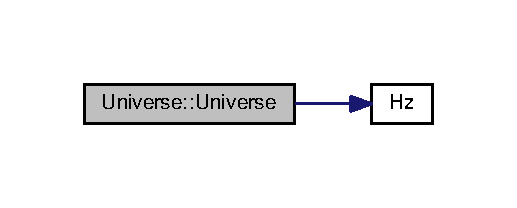
\includegraphics[width=248pt]{class_universe_a4d137a146dd3c2514dfb692dfbab6984_cgraph}
\end{center}
\end{figure}


\hypertarget{class_universe_aa8287eefad81a39bd22e4fc4b3469913}{\index{Universe@{Universe}!Universe@{Universe}}
\index{Universe@{Universe}!Universe@{Universe}}
\subsubsection[{Universe}]{\setlength{\rightskip}{0pt plus 5cm}Universe\-::\-Universe (
\begin{DoxyParamCaption}
\item[{double}]{h0}
\end{DoxyParamCaption}
)}}\label{class_universe_aa8287eefad81a39bd22e4fc4b3469913}
Creates a universe with $H_{0} = $h0 $ \ km/s/Mpc$. All other values are set to the default. 
\begin{DoxyParams}{Parameters}
{\em h0} & Units\-: $km/s/Mpc$ \\
\hline
\end{DoxyParams}


Definition at line 23 of file Universe.\-cpp.



Here is the call graph for this function\-:\nopagebreak
\begin{figure}[H]
\begin{center}
\leavevmode
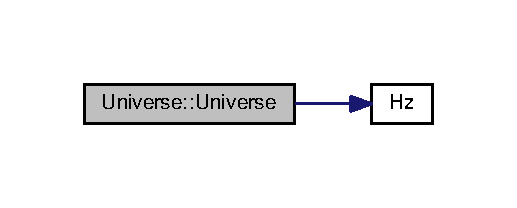
\includegraphics[width=248pt]{class_universe_aa8287eefad81a39bd22e4fc4b3469913_cgraph}
\end{center}
\end{figure}


\hypertarget{class_universe_aa3a2ada69e53bfbe237755c821110d31}{\index{Universe@{Universe}!Universe@{Universe}}
\index{Universe@{Universe}!Universe@{Universe}}
\subsubsection[{Universe}]{\setlength{\rightskip}{0pt plus 5cm}Universe\-::\-Universe (
\begin{DoxyParamCaption}
\item[{double}]{omega\-M, }
\item[{double}]{omega\-L}
\end{DoxyParamCaption}
)}}\label{class_universe_aa3a2ada69e53bfbe237755c821110d31}
Creates a universe with $\Omega_{M} =$ omega\-M and $\Omega_{\Lambda} =$ omega\-L. All other values are set to the default. 
\begin{DoxyParams}{Parameters}
{\em omega\-M} & Units\-: N\-A \\
\hline
{\em omega\-L} & Units\-: N\-A \\
\hline
\end{DoxyParams}


Definition at line 38 of file Universe.\-cpp.



Here is the call graph for this function\-:\nopagebreak
\begin{figure}[H]
\begin{center}
\leavevmode
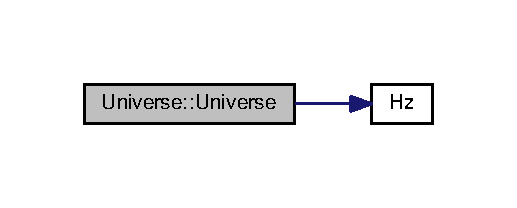
\includegraphics[width=248pt]{class_universe_aa3a2ada69e53bfbe237755c821110d31_cgraph}
\end{center}
\end{figure}


\hypertarget{class_universe_a4d57eccd5bccb65a07ee8014d874f742}{\index{Universe@{Universe}!Universe@{Universe}}
\index{Universe@{Universe}!Universe@{Universe}}
\subsubsection[{Universe}]{\setlength{\rightskip}{0pt plus 5cm}Universe\-::\-Universe (
\begin{DoxyParamCaption}
\item[{double}]{h0, }
\item[{double}]{omega\-M, }
\item[{double}]{omega\-L}
\end{DoxyParamCaption}
)}}\label{class_universe_a4d57eccd5bccb65a07ee8014d874f742}
Creates a universe with $H_{0} = $ h0 $km/s/Mpc$, $\Omega_{M} =$ omega\-M, and $\Omega_{\Lambda} =$ omega\-L. All other values are set to the default. 
\begin{DoxyParams}{Parameters}
{\em h0} & Units\-: $km/s/Mpc$ \\
\hline
{\em omega\-M} & Units\-: N\-A \\
\hline
{\em omega\-L} & Units\-: N\-A \\
\hline
\end{DoxyParams}


Definition at line 53 of file Universe.\-cpp.



Here is the call graph for this function\-:\nopagebreak
\begin{figure}[H]
\begin{center}
\leavevmode
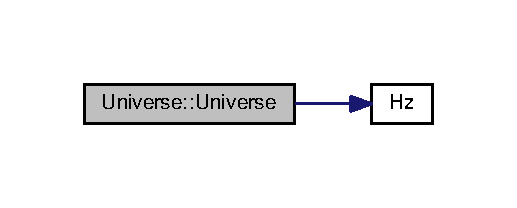
\includegraphics[width=248pt]{class_universe_a4d57eccd5bccb65a07ee8014d874f742_cgraph}
\end{center}
\end{figure}


\hypertarget{class_universe_a267e0955820c139f031d838894ae378e}{\index{Universe@{Universe}!Universe@{Universe}}
\index{Universe@{Universe}!Universe@{Universe}}
\subsubsection[{Universe}]{\setlength{\rightskip}{0pt plus 5cm}Universe\-::\-Universe (
\begin{DoxyParamCaption}
\item[{double}]{h0, }
\item[{double}]{omega\-M, }
\item[{double}]{omega\-L, }
\item[{double}]{omega\-G}
\end{DoxyParamCaption}
)}}\label{class_universe_a267e0955820c139f031d838894ae378e}
Creates a universe with $H_{0} =$ h0 $km/s/Mpc$, $\Omega_{M} =$ omega\-M, $\Omega_{\Lambda} =$ omega\-L, and $\Omega_{\gamma} =$ omega\-G. All other values are set to the default. 
\begin{DoxyParams}{Parameters}
{\em h0} & Units\-: $km/s/Mpc$ \\
\hline
{\em omega\-M} & Units\-: N\-A \\
\hline
{\em omega\-L} & Units\-: N\-A \\
\hline
{\em omega\-G} & Units\-: N\-A \\
\hline
\end{DoxyParams}


Definition at line 68 of file Universe.\-cpp.



Here is the call graph for this function\-:\nopagebreak
\begin{figure}[H]
\begin{center}
\leavevmode
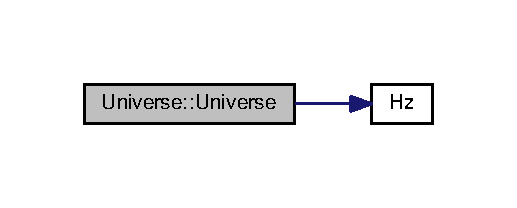
\includegraphics[width=248pt]{class_universe_a267e0955820c139f031d838894ae378e_cgraph}
\end{center}
\end{figure}


\hypertarget{class_universe_a6deb72c0b3ae4774ca3608451fce7ce6}{\index{Universe@{Universe}!Universe@{Universe}}
\index{Universe@{Universe}!Universe@{Universe}}
\subsubsection[{Universe}]{\setlength{\rightskip}{0pt plus 5cm}Universe\-::\-Universe (
\begin{DoxyParamCaption}
\item[{const {\bf Universe} \&}]{orig}
\end{DoxyParamCaption}
)}}\label{class_universe_a6deb72c0b3ae4774ca3608451fce7ce6}
Creates a copy of \hyperlink{class_universe}{Universe} orig. 

Definition at line 83 of file Universe.\-cpp.

\hypertarget{class_universe_af63f567a85ac8c644c446b1ff53995cf}{\index{Universe@{Universe}!$\sim$\-Universe@{$\sim$\-Universe}}
\index{$\sim$\-Universe@{$\sim$\-Universe}!Universe@{Universe}}
\subsubsection[{$\sim$\-Universe}]{\setlength{\rightskip}{0pt plus 5cm}Universe\-::$\sim$\-Universe (
\begin{DoxyParamCaption}
{}
\end{DoxyParamCaption}
)\hspace{0.3cm}{\ttfamily [default]}}}\label{class_universe_af63f567a85ac8c644c446b1ff53995cf}
Destroys universe. 

\subsection{Member Function Documentation}
\hypertarget{class_universe_a45c5e437ac9f03652f753a5d86f314f0}{\index{Universe@{Universe}!operator()@{operator()}}
\index{operator()@{operator()}!Universe@{Universe}}
\subsubsection[{operator()}]{\setlength{\rightskip}{0pt plus 5cm}void Universe\-::operator() (
\begin{DoxyParamCaption}
\item[{const vector$<$ double $>$ \&}]{x, }
\item[{vector$<$ double $>$ \&}]{dxdt, }
\item[{const double}]{t}
\end{DoxyParamCaption}
)}}\label{class_universe_a45c5e437ac9f03652f753a5d86f314f0}


Definition at line 108 of file Universe.\-cpp.

\hypertarget{class_universe_a446172cfdff7993bf67e0ca200d784e0}{\index{Universe@{Universe}!operator=@{operator=}}
\index{operator=@{operator=}!Universe@{Universe}}
\subsubsection[{operator=}]{\setlength{\rightskip}{0pt plus 5cm}{\bf Universe} \& Universe\-::operator= (
\begin{DoxyParamCaption}
\item[{const {\bf Universe} \&}]{orig}
\end{DoxyParamCaption}
)}}\label{class_universe_a446172cfdff7993bf67e0ca200d784e0}
Makes universe U equal to universe orig. Two universes are equal if all the cosmological parameters are the same. 
\begin{DoxyParams}{Parameters}
{\em orig} & Units\-: N\-A \\
\hline
\end{DoxyParams}


Definition at line 95 of file Universe.\-cpp.

\hypertarget{class_universe_a8f7d3385d0a7adf659b4a68300f744e6}{\index{Universe@{Universe}!operator==@{operator==}}
\index{operator==@{operator==}!Universe@{Universe}}
\subsubsection[{operator==}]{\setlength{\rightskip}{0pt plus 5cm}bool Universe\-::operator== (
\begin{DoxyParamCaption}
\item[{const {\bf Universe} \&}]{univ1}
\end{DoxyParamCaption}
)}}\label{class_universe_a8f7d3385d0a7adf659b4a68300f744e6}
Checks to see if universe U is equal to universe univ1. Two universes are equal if all the cosmological parameters are the same. 
\begin{DoxyParams}{Parameters}
{\em univ1} & Units\-: N\-A \\
\hline
\end{DoxyParams}


\subsection{Friends And Related Function Documentation}
\hypertarget{class_universe_a0480ccbf91fcb415696ba466a7ae1401}{\index{Universe@{Universe}!Equatorial@{Equatorial}}
\index{Equatorial@{Equatorial}!Universe@{Universe}}
\subsubsection[{Equatorial}]{\setlength{\rightskip}{0pt plus 5cm}friend class {\bf Equatorial}\hspace{0.3cm}{\ttfamily [friend]}}}\label{class_universe_a0480ccbf91fcb415696ba466a7ae1401}


Definition at line 24 of file Universe.\-hpp.

\hypertarget{class_universe_a2ba8175dcf9e583c18ffef6d19ee6e9d}{\index{Universe@{Universe}!Galactic@{Galactic}}
\index{Galactic@{Galactic}!Universe@{Universe}}
\subsubsection[{Galactic}]{\setlength{\rightskip}{0pt plus 5cm}friend class {\bf Galactic}\hspace{0.3cm}{\ttfamily [friend]}}}\label{class_universe_a2ba8175dcf9e583c18ffef6d19ee6e9d}


Definition at line 25 of file Universe.\-hpp.

\hypertarget{class_universe_ab594011d9eb73ce33234ae0e11850252}{\index{Universe@{Universe}!Kepler\-Obj@{Kepler\-Obj}}
\index{Kepler\-Obj@{Kepler\-Obj}!Universe@{Universe}}
\subsubsection[{Kepler\-Obj}]{\setlength{\rightskip}{0pt plus 5cm}friend class {\bf Kepler\-Obj}\hspace{0.3cm}{\ttfamily [friend]}}}\label{class_universe_ab594011d9eb73ce33234ae0e11850252}


Definition at line 27 of file Universe.\-hpp.

\hypertarget{class_universe_a438b315afa8c872673a2dc740ac8243d}{\index{Universe@{Universe}!Obj@{Obj}}
\index{Obj@{Obj}!Universe@{Universe}}
\subsubsection[{Obj}]{\setlength{\rightskip}{0pt plus 5cm}friend class {\bf Obj}\hspace{0.3cm}{\ttfamily [friend]}}}\label{class_universe_a438b315afa8c872673a2dc740ac8243d}


Definition at line 26 of file Universe.\-hpp.

\hypertarget{class_universe_a923ffb102f2f1cf8c018e2fdab71e759}{\index{Universe@{Universe}!operator!=@{operator!=}}
\index{operator!=@{operator!=}!Universe@{Universe}}
\subsubsection[{operator!=}]{\setlength{\rightskip}{0pt plus 5cm}bool operator!= (
\begin{DoxyParamCaption}
\item[{const {\bf Universe} \&}]{univ1, }
\item[{const {\bf Universe} \&}]{univ2}
\end{DoxyParamCaption}
)\hspace{0.3cm}{\ttfamily [friend]}}}\label{class_universe_a923ffb102f2f1cf8c018e2fdab71e759}


Definition at line 131 of file Universe.\-cpp.

\hypertarget{class_universe_ae6d5ff462dc8f2a42c1c89dfbb045a70}{\index{Universe@{Universe}!operator$<$@{operator$<$}}
\index{operator$<$@{operator$<$}!Universe@{Universe}}
\subsubsection[{operator$<$}]{\setlength{\rightskip}{0pt plus 5cm}bool operator$<$ (
\begin{DoxyParamCaption}
\item[{const {\bf Universe} \&}]{univ1, }
\item[{const {\bf Universe} \&}]{univ2}
\end{DoxyParamCaption}
)\hspace{0.3cm}{\ttfamily [friend]}}}\label{class_universe_ae6d5ff462dc8f2a42c1c89dfbb045a70}


Definition at line 139 of file Universe.\-cpp.

\hypertarget{class_universe_af3dca6b540cbad8426d8aae6dc1f6f32}{\index{Universe@{Universe}!operator$<$$<$@{operator$<$$<$}}
\index{operator$<$$<$@{operator$<$$<$}!Universe@{Universe}}
\subsubsection[{operator$<$$<$}]{\setlength{\rightskip}{0pt plus 5cm}ostream\& operator$<$$<$ (
\begin{DoxyParamCaption}
\item[{ostream \&}]{os, }
\item[{const {\bf Universe} \&}]{u}
\end{DoxyParamCaption}
)\hspace{0.3cm}{\ttfamily [friend]}}}\label{class_universe_af3dca6b540cbad8426d8aae6dc1f6f32}


Definition at line 168 of file Universe.\-cpp.

\hypertarget{class_universe_aedb45560ee22b1f0d1913bd40c716f3e}{\index{Universe@{Universe}!operator$<$=@{operator$<$=}}
\index{operator$<$=@{operator$<$=}!Universe@{Universe}}
\subsubsection[{operator$<$=}]{\setlength{\rightskip}{0pt plus 5cm}bool operator$<$= (
\begin{DoxyParamCaption}
\item[{const {\bf Universe} \&}]{univ1, }
\item[{const {\bf Universe} \&}]{univ2}
\end{DoxyParamCaption}
)\hspace{0.3cm}{\ttfamily [friend]}}}\label{class_universe_aedb45560ee22b1f0d1913bd40c716f3e}


Definition at line 153 of file Universe.\-cpp.

\hypertarget{class_universe_ad7426db61680a1aa7bf601a316f50296}{\index{Universe@{Universe}!operator==@{operator==}}
\index{operator==@{operator==}!Universe@{Universe}}
\subsubsection[{operator==}]{\setlength{\rightskip}{0pt plus 5cm}bool operator== (
\begin{DoxyParamCaption}
\item[{const {\bf Universe} \&}]{univ1, }
\item[{const {\bf Universe} \&}]{univ2}
\end{DoxyParamCaption}
)\hspace{0.3cm}{\ttfamily [friend]}}}\label{class_universe_ad7426db61680a1aa7bf601a316f50296}


Definition at line 123 of file Universe.\-cpp.

\hypertarget{class_universe_ac646834ee273250d89054f51c560ad90}{\index{Universe@{Universe}!operator$>$@{operator$>$}}
\index{operator$>$@{operator$>$}!Universe@{Universe}}
\subsubsection[{operator$>$}]{\setlength{\rightskip}{0pt plus 5cm}bool operator$>$ (
\begin{DoxyParamCaption}
\item[{const {\bf Universe} \&}]{univ1, }
\item[{const {\bf Universe} \&}]{univ2}
\end{DoxyParamCaption}
)\hspace{0.3cm}{\ttfamily [friend]}}}\label{class_universe_ac646834ee273250d89054f51c560ad90}


Definition at line 146 of file Universe.\-cpp.

\hypertarget{class_universe_ad2f27b03dcb666cb1e5f00840f3cffe2}{\index{Universe@{Universe}!operator$>$=@{operator$>$=}}
\index{operator$>$=@{operator$>$=}!Universe@{Universe}}
\subsubsection[{operator$>$=}]{\setlength{\rightskip}{0pt plus 5cm}bool operator$>$= (
\begin{DoxyParamCaption}
\item[{const {\bf Universe} \&}]{univ1, }
\item[{const {\bf Universe} \&}]{univ2}
\end{DoxyParamCaption}
)\hspace{0.3cm}{\ttfamily [friend]}}}\label{class_universe_ad2f27b03dcb666cb1e5f00840f3cffe2}


Definition at line 160 of file Universe.\-cpp.

\hypertarget{class_universe_ad347ea8dc2c56d9d77d9c6f673d5927e}{\index{Universe@{Universe}!operator$>$$>$@{operator$>$$>$}}
\index{operator$>$$>$@{operator$>$$>$}!Universe@{Universe}}
\subsubsection[{operator$>$$>$}]{\setlength{\rightskip}{0pt plus 5cm}istream\& operator$>$$>$ (
\begin{DoxyParamCaption}
\item[{istream \&}]{is, }
\item[{{\bf Universe} \&}]{u}
\end{DoxyParamCaption}
)\hspace{0.3cm}{\ttfamily [friend]}}}\label{class_universe_ad347ea8dc2c56d9d77d9c6f673d5927e}


Definition at line 173 of file Universe.\-cpp.

\hypertarget{class_universe_acb9341c7022366ea58f9779acad08e11}{\index{Universe@{Universe}!Spherical@{Spherical}}
\index{Spherical@{Spherical}!Universe@{Universe}}
\subsubsection[{Spherical}]{\setlength{\rightskip}{0pt plus 5cm}friend class {\bf Spherical}\hspace{0.3cm}{\ttfamily [friend]}}}\label{class_universe_acb9341c7022366ea58f9779acad08e11}


Definition at line 23 of file Universe.\-hpp.



\subsection{Member Data Documentation}
\hypertarget{class_universe_a478a9072a4445f6fc3dd9cf2bc641683}{\index{Universe@{Universe}!age\-H@{age\-H}}
\index{age\-H@{age\-H}!Universe@{Universe}}
\subsubsection[{age\-H}]{\setlength{\rightskip}{0pt plus 5cm}double Universe\-::age\-H = 0.\-0}}\label{class_universe_a478a9072a4445f6fc3dd9cf2bc641683}
$ a_{H}$ -\/ the age of the \hyperlink{class_universe}{Universe}. 

Definition at line 43 of file Universe.\-hpp.

\hypertarget{class_universe_a397c3302597d221feaaacac332837fd2}{\index{Universe@{Universe}!c@{c}}
\index{c@{c}!Universe@{Universe}}
\subsubsection[{c}]{\setlength{\rightskip}{0pt plus 5cm}constexpr double Universe\-::c = 299792458.\-0\hspace{0.3cm}{\ttfamily [static]}}}\label{class_universe_a397c3302597d221feaaacac332837fd2}
$c = 299792458.0 \ m/s$ -\/ the speed of light. 

Definition at line 40 of file Universe.\-hpp.

\hypertarget{class_universe_aa9e574f4cac819cfa806f24c24eec60e}{\index{Universe@{Universe}!dist\-H@{dist\-H}}
\index{dist\-H@{dist\-H}!Universe@{Universe}}
\subsubsection[{dist\-H}]{\setlength{\rightskip}{0pt plus 5cm}double Universe\-::dist\-H = {\bf c}/(67.\-77$\ast$1.\-0e3)}}\label{class_universe_aa9e574f4cac819cfa806f24c24eec60e}
$d_{H} = c/H_{0}$ -\/ the Hubble distance. 

Definition at line 41 of file Universe.\-hpp.

\hypertarget{class_universe_af2ce871543e110d45306c37c705b0574}{\index{Universe@{Universe}!size\-H@{size\-H}}
\index{size\-H@{size\-H}!Universe@{Universe}}
\subsubsection[{size\-H}]{\setlength{\rightskip}{0pt plus 5cm}double Universe\-::size\-H = 0.\-0}}\label{class_universe_af2ce871543e110d45306c37c705b0574}
$ s_{H}$ -\/ the size of the \hyperlink{class_universe}{Universe}. 

Definition at line 44 of file Universe.\-hpp.

\hypertarget{class_universe_a7a1b9c18475efced2a8260420dfc3911}{\index{Universe@{Universe}!time\-H@{time\-H}}
\index{time\-H@{time\-H}!Universe@{Universe}}
\subsubsection[{time\-H}]{\setlength{\rightskip}{0pt plus 5cm}double Universe\-::time\-H = (Mpc2\-Km/67.\-77)/(Yrs2\-Sec$\ast$1.\-0e9)}}\label{class_universe_a7a1b9c18475efced2a8260420dfc3911}
$t_{H} = 1/H_{0}$ -\/ the Hubble time. 

Definition at line 42 of file Universe.\-hpp.



The documentation for this class was generated from the following files\-:\begin{DoxyCompactItemize}
\item 
/home/vish/code/trunk/cpp/libcarma/include/\hyperlink{_universe_8hpp}{Universe.\-hpp}\item 
/home/vish/code/trunk/cpp/libcarma/src/\hyperlink{_universe_8cpp}{Universe.\-cpp}\end{DoxyCompactItemize}

\chapter{File Documentation}
\hypertarget{_final_analysis_8py}{\section{/home/vish/code/trunk/cpp/libcarma/\-Final\-Analysis.py File Reference}
\label{_final_analysis_8py}\index{/home/vish/code/trunk/cpp/libcarma/\-Final\-Analysis.\-py@{/home/vish/code/trunk/cpp/libcarma/\-Final\-Analysis.\-py}}
}
\subsection*{Namespaces}
\begin{DoxyCompactItemize}
\item 
\hyperlink{namespace_final_analysis}{Final\-Analysis}
\end{DoxyCompactItemize}
\subsection*{Functions}
\begin{DoxyCompactItemize}
\item 
def \hyperlink{namespace_final_analysis_aa2936d2049a535da38d4b9777acc0e22}{Final\-Analysis.\-M\-A\-D}
\end{DoxyCompactItemize}
\subsection*{Variables}
\begin{DoxyCompactItemize}
\item 
int \hyperlink{namespace_final_analysis_a8237fbcf96157871ca15161b8c911d6a}{Final\-Analysis.\-s1} = 2
\item 
int \hyperlink{namespace_final_analysis_a6e5fab082186d13ccafedfe0f8a36fd3}{Final\-Analysis.\-s2} = 9
\item 
float \hyperlink{namespace_final_analysis_abc30d10b634674cdb4958c494025d3ce}{Final\-Analysis.\-fwid} = 8.\-5
\item 
float \hyperlink{namespace_final_analysis_a655a72c0122ba74cfe825ce4a0fd48e0}{Final\-Analysis.\-fhgt} = 5.\-25
\item 
int \hyperlink{namespace_final_analysis_ae1013699910a86a41a0a50eeba068419}{Final\-Analysis.\-dots\-Per\-Inch} = 600
\item 
int \hyperlink{namespace_final_analysis_ab8aad06278d0423ea7c2ef145097954b}{Final\-Analysis.\-nbins} = 100
\item 
float \hyperlink{namespace_final_analysis_aad4e1075c61393b18c1fe9942acd8789}{Final\-Analysis.\-sec\-Per\-Sidereal\-Day} = 86164.\-0905
\item 
float \hyperlink{namespace_final_analysis_ae7544fab9b92313efce519dfcbe443ef}{Final\-Analysis.\-int\-Time} = 6.\-019802903
\item 
float \hyperlink{namespace_final_analysis_a52de26ab1dba066ec7d2b10dd3bd8544}{Final\-Analysis.\-read\-Time} = 0.\-5189485261
\item 
int \hyperlink{namespace_final_analysis_a9481028e551e6a7d0abf48c81f22cf86}{Final\-Analysis.\-num\-Int\-L\-C} = 270
\item 
tuple \hyperlink{namespace_final_analysis_aa27dc5884cf09a2ac3f1fb3489bb359b}{Final\-Analysis.\-deltat} = (num\-Int\-L\-C$\ast$(int\-Time+\hyperlink{_constants_8cpp_abd52f1ed1ece35cffe3fc3e4180ca0f3}{read\-Time}))
\item 
string \hyperlink{namespace_final_analysis_abf963966146e1751a9c7aeb6a4df238a}{Final\-Analysis.\-Tri\-File\-Path} = base\-Path+'mcmc\-Out\-\_\-\%d\-\_\-\%d.\-dat'
\item 
tuple \hyperlink{namespace_final_analysis_a05fafd47a96b32e6c3dc6e30dac35672}{Final\-Analysis.\-Tri\-File} = open(Tri\-File\-Path)
\item 
tuple \hyperlink{namespace_final_analysis_a7c83462f12c6791e4425510419b04eb4}{Final\-Analysis.\-line} = Tri\-File.\-readline()
\item 
tuple \hyperlink{namespace_final_analysis_acd9913ccc0f466893ae0a193d0a17388}{Final\-Analysis.\-values} = line.\-split()
\item 
tuple \hyperlink{namespace_final_analysis_a11e023099f2819c75bd7ecb02c7671c3}{Final\-Analysis.\-nsteps} = int(values\mbox{[}1\mbox{]})
\item 
tuple \hyperlink{namespace_final_analysis_aa7ae3a71cd02bd6488a119cf3041b24e}{Final\-Analysis.\-nwalkers} = int(values\mbox{[}1\mbox{]})
\item 
tuple \hyperlink{namespace_final_analysis_ae4b307ed4519c8b02333909f683f76d6}{Final\-Analysis.\-ndim} = int(values\mbox{[}1\mbox{]})
\item 
tuple \hyperlink{namespace_final_analysis_abcbb56dee8740482b79123ed446a959e}{Final\-Analysis.\-walkers} = np.\-zeros((nsteps,nwalkers,ndim))
\item 
tuple \hyperlink{namespace_final_analysis_a3df48ee06c31fdb1cf340b4fbcf9f9f6}{Final\-Analysis.\-deviances} = np.\-zeros((nsteps,nwalkers))
\item 
tuple \hyperlink{namespace_final_analysis_a84eaae13a656db02c1fb234b67fa211f}{Final\-Analysis.\-median\-Walker} = np.\-zeros((nsteps,ndim))
\item 
tuple \hyperlink{namespace_final_analysis_ac362b5ee700f3dc97ef8f58b9c95f019}{Final\-Analysis.\-median\-Dev\-Walker} = np.\-zeros((nsteps,ndim))
\item 
tuple \hyperlink{namespace_final_analysis_a221de63368631e4bf8a334f9f0b4fcdb}{Final\-Analysis.\-step\-Arr} = np.\-arange(nsteps)
\item 
list \hyperlink{namespace_final_analysis_aa61b8c8a4b0a4c679d09737c3ae4c39c}{Final\-Analysis.\-samples} = walkers\mbox{[}chop\-:,\-:,\-:\mbox{]}
\item 
list \hyperlink{namespace_final_analysis_a0a76ade78d1bb36b45ca6950b6a340a9}{Final\-Analysis.\-sample\-Deviances} = deviances\mbox{[}chop\-:,\-:\mbox{]}
\item 
float \hyperlink{namespace_final_analysis_a68c248ca9c873f73a8e36a8ee251cb55}{Final\-Analysis.\-D\-I\-C} = 0.\-5
\item 
tuple \hyperlink{namespace_final_analysis_ad0acefcc028d6b5ed6a5df8a33837c93}{Final\-Analysis.\-lbls} = list()
\item 
tuple \hyperlink{namespace_final_analysis_ac46e153da6c229304def2ef1594ad6d0}{Final\-Analysis.\-sorted\-D\-I\-C\-Vals} = sorted(dict\-D\-I\-C.\-items(),key=operator.\-itemgetter(1))
\item 
tuple \hyperlink{namespace_final_analysis_a4cb7be1a71ae9339b38be19665d4816b}{Final\-Analysis.\-p\-Best} = int(sorted\-D\-I\-C\-Vals\mbox{[}0\mbox{]}\mbox{[}0\mbox{]}.split()\mbox{[}0\mbox{]})
\item 
tuple \hyperlink{namespace_final_analysis_a52c1bec46dd832ef73e9e1d21d28155b}{Final\-Analysis.\-q\-Best} = int(sorted\-D\-I\-C\-Vals\mbox{[}0\mbox{]}\mbox{[}0\mbox{]}.split()\mbox{[}1\mbox{]})
\item 
float \hyperlink{namespace_final_analysis_a503e1ab9c53535c8cf3182b5bd683239}{Final\-Analysis.\-Rel\-Prob\-Of\-Min\-Inf\-Loss} = 100.\-0
\item 
string \hyperlink{namespace_final_analysis_a8286808e6828d6957c0b9b9159314b08}{Final\-Analysis.\-best\-File\-Path} = base\-Path+'mcmc\-Out\-\_\-\%d\-\_\-\%d.\-dat'
\item 
tuple \hyperlink{namespace_final_analysis_a2990113fcd9a31e44606ce17d678f9fb}{Final\-Analysis.\-best\-File} = open(best\-File\-Path)
\item 
tuple \hyperlink{namespace_final_analysis_a02480d595c49c0f2494cb9b94dc93ad8}{Final\-Analysis.\-rand\-Step} = r.\-randint(chop,nsteps-\/1)
\item 
tuple \hyperlink{namespace_final_analysis_a9dab2cf8612b12f65a094eac2c433ac1}{Final\-Analysis.\-rand\-Walker} = r.\-randint(0,nwalkers-\/1)
\item 
list \hyperlink{namespace_final_analysis_a8d45e2b4a2cbacf49eab526ac11ecc77}{Final\-Analysis.\-phi\-Best} = \mbox{[}dim for dim in walkers\mbox{[}rand\-Step,rand\-Walker,1\-:p\-Best+1\mbox{]}.tolist()\mbox{]}
\item 
list \hyperlink{namespace_final_analysis_ae73eb98f29c137ecea3dc1021ba665b5}{Final\-Analysis.\-theta\-Best} = \mbox{[}dim for dim in walkers\mbox{[}rand\-Step,rand\-Walker,p\-Best+1\-:p\-Best+q\-Best+1\mbox{]}\mbox{]}
\item 
list \hyperlink{namespace_final_analysis_ab9b839125655898989c2bba36c4b2d82}{Final\-Analysis.\-sigma\-Best} = walkers\mbox{[}rand\-Step,rand\-Walker,0\mbox{]}
\item 
string \hyperlink{namespace_final_analysis_ad8aaf10ff3415780cc1c8fcd7990395a}{Final\-Analysis.\-y\-File\-Path} = base\-Path+'y.\-dat'
\item 
tuple \hyperlink{namespace_final_analysis_a73049f17326c78323b2344dc7cb4c05d}{Final\-Analysis.\-y\-File} = open(y\-File\-Path)
\item 
tuple \hyperlink{namespace_final_analysis_ab417da76d397a990dd95199dccc1b61b}{Final\-Analysis.\-num\-Pts} = int(values\mbox{[}1\mbox{]})
\item 
tuple \hyperlink{namespace_final_analysis_a38df881ad911780b915aa9e19ebb7dc6}{Final\-Analysis.\-num\-Obs} = int(values\mbox{[}1\mbox{]})
\item 
tuple \hyperlink{namespace_final_analysis_a1c2fa47f2afa602b9c2d25ec8580ff42}{Final\-Analysis.\-mean\-Y} = float(values\mbox{[}1\mbox{]})
\item 
tuple \hyperlink{namespace_final_analysis_a90758b7deb047594ad04ead892b7627e}{Final\-Analysis.\-t} = np.\-zeros((num\-Pts,2))
\item 
tuple \hyperlink{namespace_final_analysis_af061a7f615d51259e7a6720b6f39f02d}{Final\-Analysis.\-y} = np.\-zeros((num\-Pts,2))
\item 
tuple \hyperlink{namespace_final_analysis_a94fb4e8e60fe4cb0595dee2bbaf20c81}{Final\-Analysis.\-mask} = np.\-zeros(num\-Pts)
\item 
tuple \hyperlink{namespace_final_analysis_a53f403035b6d6abe6c7e2d7c07601b1d}{Final\-Analysis.\-x} = np.\-zeros((num\-Pts,2))
\item 
tuple \hyperlink{namespace_final_analysis_a8fb9ac591a57f2affeeb677906de4d5f}{Final\-Analysis.\-v} = np.\-zeros((num\-Pts,2))
\item 
tuple \hyperlink{namespace_final_analysis_a887a21357f13ebf746beb132e8508849}{Final\-Analysis.\-Ln\-Like} = K\-F.\-get\-Ln\-Like(y,mask,X,P,X\-Minus,P\-Minus,F,I,D,Q,H,R,K)
\item 
tuple \hyperlink{namespace_final_analysis_a7071cf368ec253b5f7165fa535e161ef}{Final\-Analysis.\-y\-Max} = np.\-max(y\mbox{[}np.\-nonzero(y\mbox{[}\-:,0\mbox{]}),0\mbox{]})
\item 
tuple \hyperlink{namespace_final_analysis_a542cfbfe4821ac9a631cbe8102ad7de6}{Final\-Analysis.\-y\-Min} = np.\-min(y\mbox{[}np.\-nonzero(y\mbox{[}\-:,0\mbox{]}),0\mbox{]})
\item 
tuple \hyperlink{namespace_final_analysis_a1876ad5867611d2150568c7311e8badb}{Final\-Analysis.\-v\-Max} = np.\-std(v\mbox{[}np.\-nonzero(v\mbox{[}\-:,0\mbox{]}),0\mbox{]})
\item 
tuple \hyperlink{namespace_final_analysis_a5dff2737a91aa5a7c56b78a13ebf95ec}{Final\-Analysis.\-v\-Min} = -\/np.\-std(v\mbox{[}np.\-nonzero(v\mbox{[}\-:,0\mbox{]}),0\mbox{]})
\item 
int \hyperlink{namespace_final_analysis_afbe11458d00db6f07dc367e9d9074744}{Final\-Analysis.\-n\-Bins} = 50
\item 
tuple \hyperlink{namespace_final_analysis_ae53b90e1254d309f41585c93c7d59100}{Final\-Analysis.\-bin\-Max} = np.\-nanmax(bin\-Vals)
\item 
tuple \hyperlink{namespace_final_analysis_af73c4fbd388650228620f11e8128489b}{Final\-Analysis.\-new\-Bin\-Vals} = np.\-zeros(n\-Bins)
\item 
tuple \hyperlink{namespace_final_analysis_ac7e5340352eec13fbd15cb78ce1d7c13}{Final\-Analysis.\-new\-Bin\-Errors} = np.\-zeros(n\-Bins)
\item 
tuple \hyperlink{namespace_final_analysis_a3e720a14f79520011003b9f32ec0e4b2}{Final\-Analysis.\-t\-Max} = np.\-nanmax(t\mbox{[}\-:,1\mbox{]})
\item 
tuple \hyperlink{namespace_final_analysis_ac252eee289b29b77df2090f24e7f6dfb}{Final\-Analysis.\-bin\-Width} = np.\-asscalar(bin\-Edges\mbox{[}1\mbox{]}-\/bin\-Edges\mbox{[}0\mbox{]})
\end{DoxyCompactItemize}

\hypertarget{_get_all_data_8py}{\section{/home/vish/code/trunk/cpp/libcarma/\-Get\-All\-Data.py File Reference}
\label{_get_all_data_8py}\index{/home/vish/code/trunk/cpp/libcarma/\-Get\-All\-Data.\-py@{/home/vish/code/trunk/cpp/libcarma/\-Get\-All\-Data.\-py}}
}
\subsection*{Namespaces}
\begin{DoxyCompactItemize}
\item 
\hyperlink{namespace_get_all_data}{Get\-All\-Data}
\end{DoxyCompactItemize}
\subsection*{Variables}
\begin{DoxyCompactItemize}
\item 
string \hyperlink{namespace_get_all_data_aa7dab644473a8e6caaa150aa36384dbe}{Get\-All\-Data.\-lightcurves\-Path} = 'http\-://archive.\-stsci.\-edu/pub/kepler/lightcurves/'
\item 
string \hyperlink{namespace_get_all_data_a45b4d0dc9728eff931ef547819c19225}{Get\-All\-Data.\-target\-\_\-pixel\-\_\-files\-Path} = 'http\-://archive.\-stsci.\-edu/pub/kepler/target\-\_\-pixel\-\_\-files/'
\item 
string \hyperlink{namespace_get_all_data_a0d44f716af41966e5d4c1e8ec5daca53}{Get\-All\-Data.\-cbv\-Path} = 'http\-://archive.\-stsci.\-edu/pub/kepler/cbv/'
\item 
tuple \hyperlink{namespace_get_all_data_a8ff73cf768ddd833d026b762528dc864}{Get\-All\-Data.\-data\-Folder} = str(sys.\-argv\mbox{[}1\mbox{]})
\item 
string \hyperlink{namespace_get_all_data_a651d69300ed082b3426d3910b6c6a5f7}{Get\-All\-Data.\-target\-List\-File} = data\-Folder+'kplr\-\_\-target\-List.\-dat'
\item 
string \hyperlink{namespace_get_all_data_a92d210ac17aea3c86c2cae13d5dcf53a}{Get\-All\-Data.\-cbv\-Folder} = data\-Folder+'cbv/'
\item 
tuple \hyperlink{namespace_get_all_data_ac340b879890051d52eef59bb312d86c6}{Get\-All\-Data.\-cbvpath} = urllib2.\-urlopen(cbv\-Path)
\item 
tuple \hyperlink{namespace_get_all_data_aa3f14258ba79c9dd527fc1805b92c818}{Get\-All\-Data.\-string} = cbvpath.\-read()
\item 
tuple \hyperlink{namespace_get_all_data_ab13b78016ebaf3b18c13c40b75b9ae3a}{Get\-All\-Data.\-cbv\-Pattern} = re.\-compile('kplr' + '\mbox{[}0-\/9\mbox{]}$\ast$-\/q\mbox{[}0-\/9\mbox{]}$\ast$-\/d\mbox{[}0-\/9\mbox{]}$\ast$\-\_\-lcbv.\-fits')
\item 
tuple \hyperlink{namespace_get_all_data_aef4e9610ed4d2405e028274abbfcdb43}{Get\-All\-Data.\-cbv\-List} = cbv\-Pattern.\-findall(string)
\item 
tuple \hyperlink{namespace_get_all_data_a59840d46d0e238ee525782c0fbe13eeb}{Get\-All\-Data.\-remote\-C\-B\-V\-File} = urllib2.\-urlopen(cbv\-Path + cbv\-List\mbox{[}2$\ast$i\mbox{]})
\item 
tuple \hyperlink{namespace_get_all_data_a48b2086a8ab4a4eb4383aaa810014866}{Get\-All\-Data.\-local\-C\-B\-V\-File} = open(cbv\-Folder + cbv\-List\mbox{[}2$\ast$i\mbox{]},'wb')
\item 
tuple \hyperlink{namespace_get_all_data_a7f0291de88ec75252bb7cfaa9a33997e}{Get\-All\-Data.\-t\-L\-File} = open(target\-List\-File)
\item 
tuple \hyperlink{namespace_get_all_data_ae7c93a35b37e6a7e1f63026786f921e3}{Get\-All\-Data.\-target} = target.\-rstrip('\textbackslash{}n')
\item 
\hyperlink{namespace_get_all_data_ad1a3a2da71089668ef951488bd43ec72}{Get\-All\-Data.\-obj\-Folder} = data\-Folder+target
\item 
string \hyperlink{namespace_get_all_data_a16ca85b9e5a52cb403c24f90f47e5380}{Get\-All\-Data.\-F\-I\-T\-S\-Folder} = obj\-Folder+'/llc/'
\item 
string \hyperlink{namespace_get_all_data_ab8e095b44d1d2a618b9f44a372540200}{Get\-All\-Data.\-sim\-Folder} = obj\-Folder+'/sim/'
\item 
string \hyperlink{namespace_get_all_data_a3f0df6e75a64830be35cfc3f992806c4}{Get\-All\-Data.\-lpdtarg\-Folder} = obj\-Folder+'/lpd-\/targ/'
\item 
list \hyperlink{namespace_get_all_data_a0ad0a5c98585457adf46115ebccbba6d}{Get\-All\-Data.\-X\-X\-X\-X} = target\mbox{[}4\-:8\mbox{]}
\item 
list \hyperlink{namespace_get_all_data_a8ae2235ff0e5280acf89f07808293bda}{Get\-All\-Data.\-K\-K\-K\-K\-K\-K\-K\-K\-K} = target\mbox{[}4\-:13\mbox{]}
\item 
tuple \hyperlink{namespace_get_all_data_ae1e57e5321d57891fb95a9c9326c9713}{Get\-All\-Data.\-urlpath} = urllib2.\-urlopen(lightcurves\-Path + X\-X\-X\-X + '/' + K\-K\-K\-K\-K\-K\-K\-K\-K)
\item 
tuple \hyperlink{namespace_get_all_data_a2dafe0984549f093bb5d258640946102}{Get\-All\-Data.\-targpath} = urllib2.\-urlopen(target\-\_\-pixel\-\_\-files\-Path + X\-X\-X\-X + '/' + K\-K\-K\-K\-K\-K\-K\-K\-K)
\item 
tuple \hyperlink{namespace_get_all_data_a6125644c05ef4f47c70dee8f9f271b21}{Get\-All\-Data.\-string\-Targ} = targpath.\-read()
\item 
tuple \hyperlink{namespace_get_all_data_a826165aca23510d517a06f85902411be}{Get\-All\-Data.\-quarter\-Pattern} = re.\-compile(target + '-\/\mbox{[}0-\/9\mbox{]}$\ast$\-\_\-llc.\-fits')
\item 
tuple \hyperlink{namespace_get_all_data_ad05a0da5848b788cf7824b79fa516b64}{Get\-All\-Data.\-targ\-Pattern} = re.\-compile(target + '-\/\mbox{[}0-\/9\mbox{]}$\ast$\-\_\-lpd-\/targ.\-fits.\-gz')
\item 
tuple \hyperlink{namespace_get_all_data_a05b955962336cb4b084d9ebadce6bebc}{Get\-All\-Data.\-quarter\-List} = quarter\-Pattern.\-findall(string)
\item 
tuple \hyperlink{namespace_get_all_data_a0e405ac3485c0d9036936f1e1639d262}{Get\-All\-Data.\-targ\-List} = targ\-Pattern.\-findall(string\-Targ)
\item 
string \hyperlink{namespace_get_all_data_ac9174f2a0b0215a84e06e5f8a4f5e5e6}{Get\-All\-Data.\-epoch\-List\-File} = obj\-Folder+'/'
\item 
tuple \hyperlink{namespace_get_all_data_aaf35a1611b07a1bc49bb090dccfaef8e}{Get\-All\-Data.\-e\-L\-File} = open(epoch\-List\-File,'w')
\item 
tuple \hyperlink{namespace_get_all_data_abb46709e621fe2edfea6055c1749afd5}{Get\-All\-Data.\-num\-Quarters} = len(quarter\-List)
\item 
string \hyperlink{namespace_get_all_data_acc2308c98b84b6b6eebcc695fff211ef}{Get\-All\-Data.\-e\-L\-File\-Line} = '\%s.\-dat\textbackslash{}n'
\item 
tuple \hyperlink{namespace_get_all_data_af072517ff6c21d5eab5ab2b237b0baf6}{Get\-All\-Data.\-remote\-Quarter\-File} = urllib2.\-urlopen(lightcurves\-Path + X\-X\-X\-X + '/' + K\-K\-K\-K\-K\-K\-K\-K\-K + '/' + quarter\-List\mbox{[}2$\ast$i\mbox{]})
\item 
tuple \hyperlink{namespace_get_all_data_a7b84aca19fc066108a7f1216a37d8bc2}{Get\-All\-Data.\-remote\-Targ\-File} = urllib2.\-urlopen(target\-\_\-pixel\-\_\-files\-Path + X\-X\-X\-X + '/' + K\-K\-K\-K\-K\-K\-K\-K\-K + '/' + targ\-List\mbox{[}2$\ast$i\mbox{]})
\item 
tuple \hyperlink{namespace_get_all_data_a877740889eb38000b292aaee018666fb}{Get\-All\-Data.\-local\-Quarter\-File} = open(F\-I\-T\-S\-Folder + quarter\-List\mbox{[}2$\ast$i\mbox{]},'wb')
\item 
tuple \hyperlink{namespace_get_all_data_a5da9f0ddc286550f618680b99a09f13e}{Get\-All\-Data.\-local\-Targ\-File} = open(lpdtarg\-Folder + targ\-List\mbox{[}2$\ast$i\mbox{]},'wb')
\end{DoxyCompactItemize}

\hypertarget{_acquire_8hpp}{\section{/home/vish/code/trunk/cpp/libcarma/include/\-Acquire.hpp File Reference}
\label{_acquire_8hpp}\index{/home/vish/code/trunk/cpp/libcarma/include/\-Acquire.\-hpp@{/home/vish/code/trunk/cpp/libcarma/include/\-Acquire.\-hpp}}
}
{\ttfamily \#include $<$cstdlib$>$}\\*
{\ttfamily \#include $<$iostream$>$}\\*
{\ttfamily \#include $<$limits$>$}\\*
{\ttfamily \#include $<$string$>$}\\*
{\ttfamily \#include $<$sstream$>$}\\*
{\ttfamily \#include $<$boost/system/error\-\_\-code.\-hpp$>$}\\*
{\ttfamily \#include $<$boost/system/system\-\_\-error.\-hpp$>$}\\*
{\ttfamily \#include $<$boost/system/linux\-\_\-error.\-hpp$>$}\\*
{\ttfamily \#include $<$boost/filesystem.\-hpp$>$}\\*
{\ttfamily \#include $<$boost/io/detail/quoted\-\_\-manip.\-hpp$>$}\\*
Include dependency graph for Acquire.\-hpp\-:\nopagebreak
\begin{figure}[H]
\begin{center}
\leavevmode
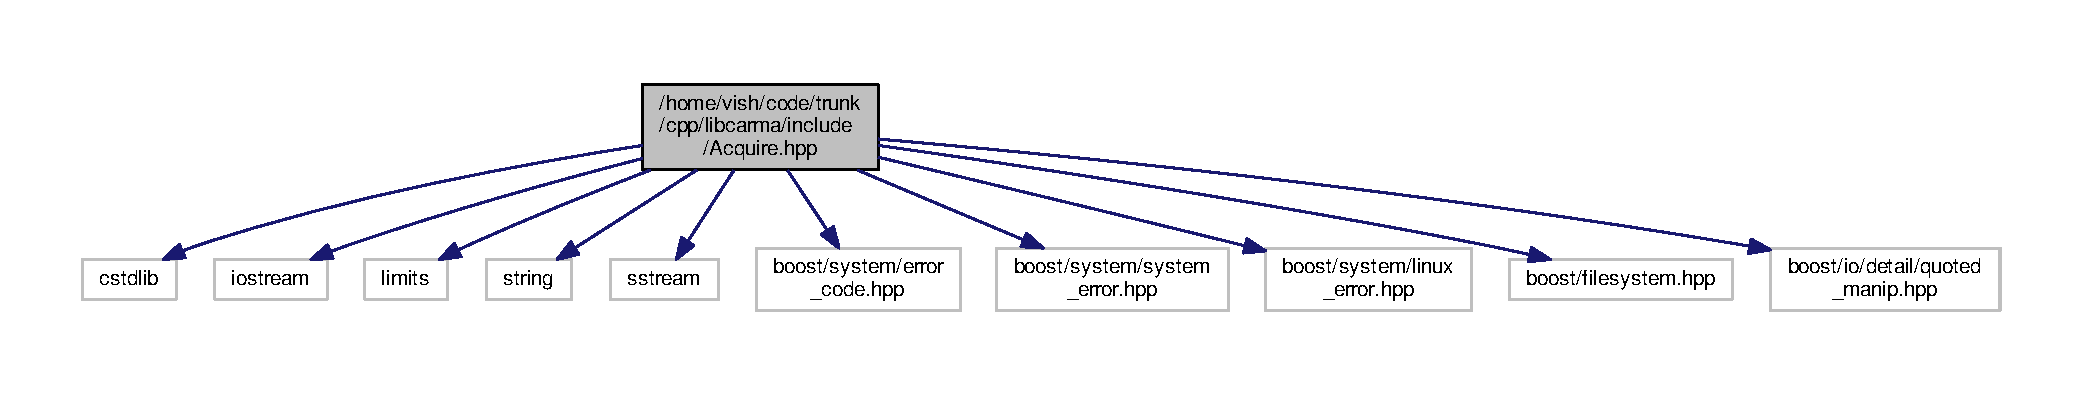
\includegraphics[width=350pt]{_acquire_8hpp__incl}
\end{center}
\end{figure}
This graph shows which files directly or indirectly include this file\-:\nopagebreak
\begin{figure}[H]
\begin{center}
\leavevmode
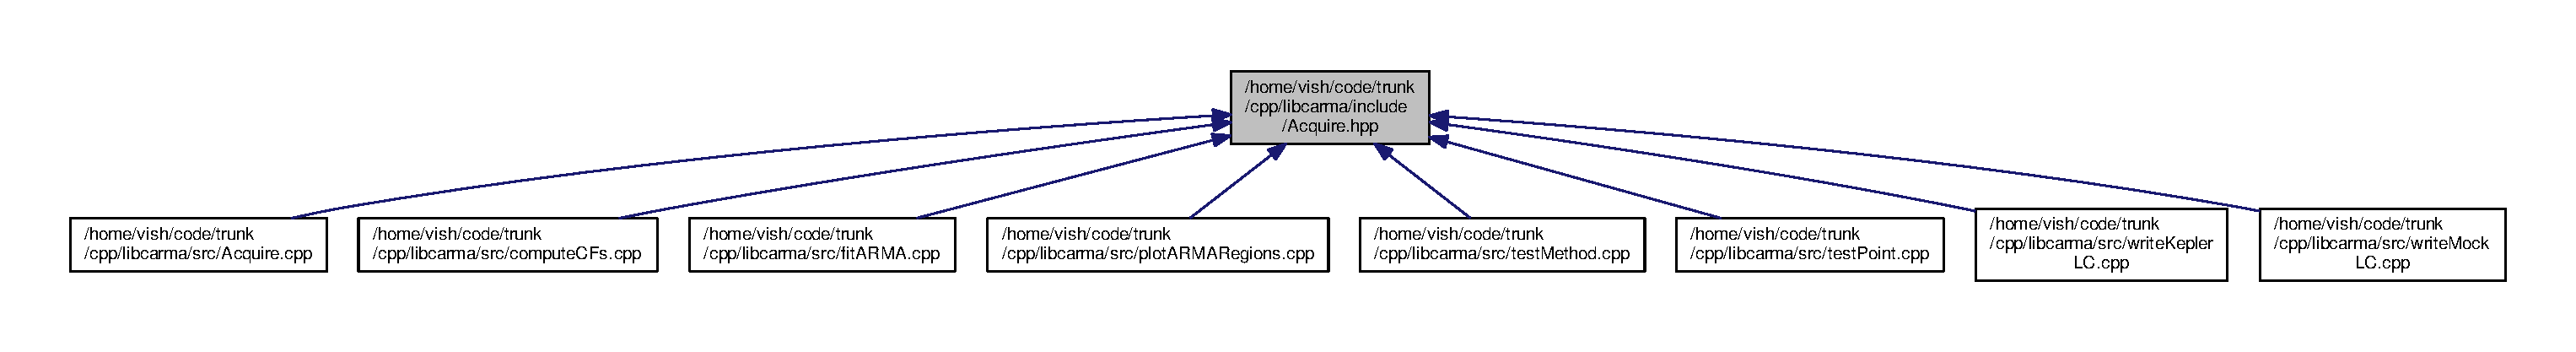
\includegraphics[width=350pt]{_acquire_8hpp__dep__incl}
\end{center}
\end{figure}
\subsection*{Functions}
\begin{DoxyCompactItemize}
\item 
{\footnotesize template$<$typename In\-Type $>$ }\\void \hyperlink{_acquire_8hpp_a42cdc40f31099f8ddbbe1334c24306c4}{Acquire\-Input} (ostream \&Os, istream \&Is, const string \&Prompt, const string \&Fail\-String, In\-Type \&Result)
\item 
{\footnotesize template$<$typename In\-Type $>$ }\\In\-Type \hyperlink{_acquire_8hpp_a76ef36c83d924d0967514c156ca762b2}{Acquire\-Input} (ostream \&Os, istream \&Is, const string \&Prompt, const string \&Fail\-String)
\item 
void \hyperlink{_acquire_8hpp_a4c4565084a152b01217e6f1650fc3450}{Acquire\-Directory} (ostream \&Os, istream \&Is, const string \&Prompt, const string \&Fail\-String, string \&Result)
\item 
void \hyperlink{_acquire_8hpp_a6d8415f6f6ba7cb8f43f36fd22d002a6}{Acquire\-File} (ostream \&Os, istream \&Is, const string \&Prompt, const string \&Fail\-String, string \&Result)
\end{DoxyCompactItemize}


\subsection{Function Documentation}
\hypertarget{_acquire_8hpp_a4c4565084a152b01217e6f1650fc3450}{\index{Acquire.\-hpp@{Acquire.\-hpp}!Acquire\-Directory@{Acquire\-Directory}}
\index{Acquire\-Directory@{Acquire\-Directory}!Acquire.hpp@{Acquire.\-hpp}}
\subsubsection[{Acquire\-Directory}]{\setlength{\rightskip}{0pt plus 5cm}void Acquire\-Directory (
\begin{DoxyParamCaption}
\item[{ostream \&}]{Os, }
\item[{istream \&}]{Is, }
\item[{const string \&}]{Prompt, }
\item[{const string \&}]{Fail\-String, }
\item[{string \&}]{Result}
\end{DoxyParamCaption}
)}}\label{_acquire_8hpp_a4c4565084a152b01217e6f1650fc3450}


Definition at line 16 of file Acquire.\-cpp.



Here is the caller graph for this function\-:\nopagebreak
\begin{figure}[H]
\begin{center}
\leavevmode
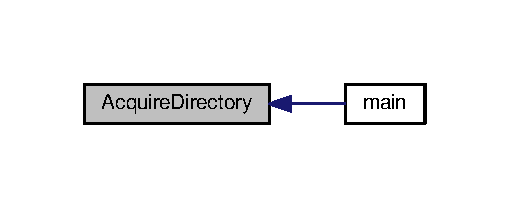
\includegraphics[width=244pt]{_acquire_8hpp_a4c4565084a152b01217e6f1650fc3450_icgraph}
\end{center}
\end{figure}


\hypertarget{_acquire_8hpp_a6d8415f6f6ba7cb8f43f36fd22d002a6}{\index{Acquire.\-hpp@{Acquire.\-hpp}!Acquire\-File@{Acquire\-File}}
\index{Acquire\-File@{Acquire\-File}!Acquire.hpp@{Acquire.\-hpp}}
\subsubsection[{Acquire\-File}]{\setlength{\rightskip}{0pt plus 5cm}void Acquire\-File (
\begin{DoxyParamCaption}
\item[{ostream \&}]{Os, }
\item[{istream \&}]{Is, }
\item[{const string \&}]{Prompt, }
\item[{const string \&}]{Fail\-String, }
\item[{string \&}]{Result}
\end{DoxyParamCaption}
)}}\label{_acquire_8hpp_a6d8415f6f6ba7cb8f43f36fd22d002a6}


Definition at line 65 of file Acquire.\-cpp.

\hypertarget{_acquire_8hpp_a42cdc40f31099f8ddbbe1334c24306c4}{\index{Acquire.\-hpp@{Acquire.\-hpp}!Acquire\-Input@{Acquire\-Input}}
\index{Acquire\-Input@{Acquire\-Input}!Acquire.hpp@{Acquire.\-hpp}}
\subsubsection[{Acquire\-Input}]{\setlength{\rightskip}{0pt plus 5cm}template$<$typename In\-Type $>$ void Acquire\-Input (
\begin{DoxyParamCaption}
\item[{ostream \&}]{Os, }
\item[{istream \&}]{Is, }
\item[{const string \&}]{Prompt, }
\item[{const string \&}]{Fail\-String, }
\item[{In\-Type \&}]{Result}
\end{DoxyParamCaption}
)}}\label{_acquire_8hpp_a42cdc40f31099f8ddbbe1334c24306c4}


Definition at line 18 of file Acquire.\-hpp.



Here is the caller graph for this function\-:\nopagebreak
\begin{figure}[H]
\begin{center}
\leavevmode
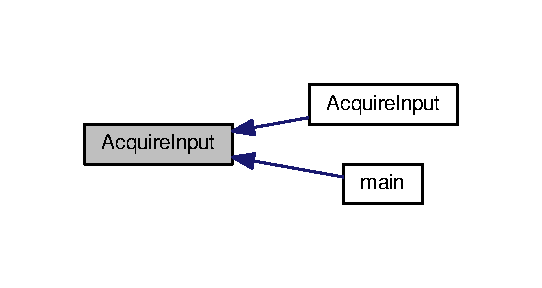
\includegraphics[width=260pt]{_acquire_8hpp_a42cdc40f31099f8ddbbe1334c24306c4_icgraph}
\end{center}
\end{figure}


\hypertarget{_acquire_8hpp_a76ef36c83d924d0967514c156ca762b2}{\index{Acquire.\-hpp@{Acquire.\-hpp}!Acquire\-Input@{Acquire\-Input}}
\index{Acquire\-Input@{Acquire\-Input}!Acquire.hpp@{Acquire.\-hpp}}
\subsubsection[{Acquire\-Input}]{\setlength{\rightskip}{0pt plus 5cm}template$<$typename In\-Type $>$ In\-Type Acquire\-Input (
\begin{DoxyParamCaption}
\item[{ostream \&}]{Os, }
\item[{istream \&}]{Is, }
\item[{const string \&}]{Prompt, }
\item[{const string \&}]{Fail\-String}
\end{DoxyParamCaption}
)}}\label{_acquire_8hpp_a76ef36c83d924d0967514c156ca762b2}


Definition at line 33 of file Acquire.\-hpp.



Here is the call graph for this function\-:\nopagebreak
\begin{figure}[H]
\begin{center}
\leavevmode
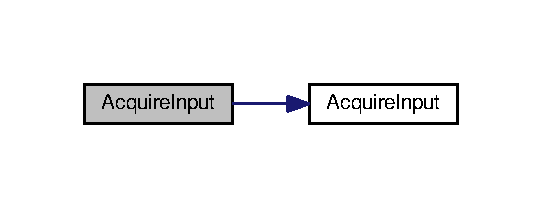
\includegraphics[width=260pt]{_acquire_8hpp_a76ef36c83d924d0967514c156ca762b2_cgraph}
\end{center}
\end{figure}



\hypertarget{_c_a_r_m_a_8hpp}{\section{/home/vish/code/trunk/cpp/libcarma/include/\-C\-A\-R\-M\-A.hpp File Reference}
\label{_c_a_r_m_a_8hpp}\index{/home/vish/code/trunk/cpp/libcarma/include/\-C\-A\-R\-M\-A.\-hpp@{/home/vish/code/trunk/cpp/libcarma/include/\-C\-A\-R\-M\-A.\-hpp}}
}
{\ttfamily \#include $<$complex$>$}\\*
{\ttfamily \#include $<$mkl\-\_\-types.\-h$>$}\\*
{\ttfamily \#include $<$mkl.\-h$>$}\\*
Include dependency graph for C\-A\-R\-M\-A.\-hpp\-:\nopagebreak
\begin{figure}[H]
\begin{center}
\leavevmode
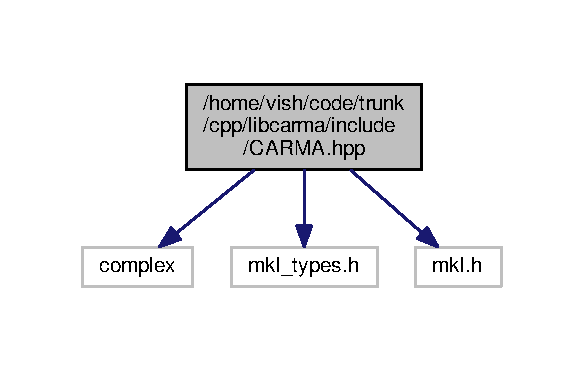
\includegraphics[width=280pt]{_c_a_r_m_a_8hpp__incl}
\end{center}
\end{figure}
This graph shows which files directly or indirectly include this file\-:\nopagebreak
\begin{figure}[H]
\begin{center}
\leavevmode
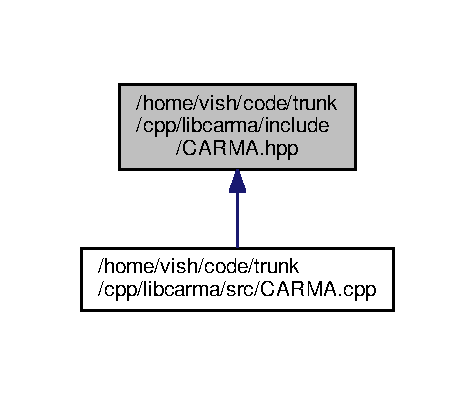
\includegraphics[width=228pt]{_c_a_r_m_a_8hpp__dep__incl}
\end{center}
\end{figure}
\subsection*{Classes}
\begin{DoxyCompactItemize}
\item 
class \hyperlink{class_c_a_r_m_a}{C\-A\-R\-M\-A}
\item 
struct \hyperlink{struct_ln_like_data}{Ln\-Like\-Data}
\item 
struct \hyperlink{struct_ln_like_args}{Ln\-Like\-Args}
\end{DoxyCompactItemize}
\subsection*{Macros}
\begin{DoxyCompactItemize}
\item 
\#define \hyperlink{_c_a_r_m_a_8hpp_a0b45f62ef34311fdb79b8de82d75c0d3}{M\-K\-L\-\_\-\-Complex8}~std\-::complex$<$float$>$
\item 
\#define \hyperlink{_c_a_r_m_a_8hpp_a1fa119034fee07a6d5449926cbb7915a}{M\-K\-L\-\_\-\-Complex16}~std\-::complex$<$double$>$
\end{DoxyCompactItemize}
\subsection*{Functions}
\begin{DoxyCompactItemize}
\item 
double \hyperlink{_c_a_r_m_a_8hpp_a9dd80aa78622e42e58063971be13e31d}{calc\-C\-A\-R\-M\-A\-Ln\-Like} (const vector$<$ double $>$ \&x, vector$<$ double $>$ \&grad, void $\ast$p2\-Args)
\item 
double \hyperlink{_c_a_r_m_a_8hpp_af732e8b64b1fb0da6791e874bd5bafa4}{calc\-C\-A\-R\-M\-A\-Ln\-Like} (double $\ast$walker\-Pos, void $\ast$vd\-Ptr2\-Ln\-Like\-Args)
\item 
double \hyperlink{_c_a_r_m_a_8hpp_ac6c51cd6959e4a7a5ec0557af951daaa}{calc\-Ln\-Like} (const vector$<$ double $>$ \&x, vector$<$ double $>$ \&grad, void $\ast$p2\-Args)
\item 
double \hyperlink{_c_a_r_m_a_8hpp_a9719ae8ef8f4ba7946a78a28412b6273}{calc\-Ln\-Like} (double $\ast$walker\-Pos, void $\ast$vd\-Ptr2\-Ln\-Like\-Args)
\item 
void \hyperlink{_c_a_r_m_a_8hpp_a52e65b8de02410a2382d1c0858c43b25}{zero\-Matrix} (int n\-Rows, int n\-Cols, int $\ast$mat)
\item 
void \hyperlink{_c_a_r_m_a_8hpp_ad06e01d494041ea73f3fb05d5208765f}{zero\-Matrix} (int n\-Rows, int n\-Cols, lapack\-\_\-int $\ast$mat)
\item 
void \hyperlink{_c_a_r_m_a_8hpp_acbdde1f5b60f8f09a2561e877f8279e5}{zero\-Matrix} (int n\-Rows, int n\-Cols, double $\ast$mat)
\item 
void \hyperlink{_c_a_r_m_a_8hpp_aff867598dfd07c509cec6da77c33fb98}{zero\-Matrix} (int n\-Rows, int n\-Cols, complex$<$ double $>$ $\ast$mat)
\item 
void \hyperlink{_c_a_r_m_a_8hpp_adaf529b8047fb0aa639f2aa494b9cfaf}{view\-Matrix} (int n\-Rows, int n\-Cols, double $\ast$mat)
\item 
void \hyperlink{_c_a_r_m_a_8hpp_ab43c14961907b75c90cee7b7fd28a3cc}{view\-Matrix} (int n\-Rows, int n\-Cols, complex$<$ double $>$ $\ast$mat)
\item 
double \hyperlink{_c_a_r_m_a_8hpp_a7a7718261954382ab26f32dae64bf3f4}{dtime} ()
\item 
void \hyperlink{_c_a_r_m_a_8hpp_a0644b006a49b595cc3e4d9cf6dff7303}{kron} (int m, int n, double $\ast$A, int p, int q, double $\ast$B, double $\ast$C)
\end{DoxyCompactItemize}


\subsection{Macro Definition Documentation}
\hypertarget{_c_a_r_m_a_8hpp_a1fa119034fee07a6d5449926cbb7915a}{\index{C\-A\-R\-M\-A.\-hpp@{C\-A\-R\-M\-A.\-hpp}!M\-K\-L\-\_\-\-Complex16@{M\-K\-L\-\_\-\-Complex16}}
\index{M\-K\-L\-\_\-\-Complex16@{M\-K\-L\-\_\-\-Complex16}!CARMA.hpp@{C\-A\-R\-M\-A.\-hpp}}
\subsubsection[{M\-K\-L\-\_\-\-Complex16}]{\setlength{\rightskip}{0pt plus 5cm}\#define M\-K\-L\-\_\-\-Complex16~std\-::complex$<$double$>$}}\label{_c_a_r_m_a_8hpp_a1fa119034fee07a6d5449926cbb7915a}


Definition at line 7 of file C\-A\-R\-M\-A.\-hpp.

\hypertarget{_c_a_r_m_a_8hpp_a0b45f62ef34311fdb79b8de82d75c0d3}{\index{C\-A\-R\-M\-A.\-hpp@{C\-A\-R\-M\-A.\-hpp}!M\-K\-L\-\_\-\-Complex8@{M\-K\-L\-\_\-\-Complex8}}
\index{M\-K\-L\-\_\-\-Complex8@{M\-K\-L\-\_\-\-Complex8}!CARMA.hpp@{C\-A\-R\-M\-A.\-hpp}}
\subsubsection[{M\-K\-L\-\_\-\-Complex8}]{\setlength{\rightskip}{0pt plus 5cm}\#define M\-K\-L\-\_\-\-Complex8~std\-::complex$<$float$>$}}\label{_c_a_r_m_a_8hpp_a0b45f62ef34311fdb79b8de82d75c0d3}


Definition at line 6 of file C\-A\-R\-M\-A.\-hpp.



\subsection{Function Documentation}
\hypertarget{_c_a_r_m_a_8hpp_a9dd80aa78622e42e58063971be13e31d}{\index{C\-A\-R\-M\-A.\-hpp@{C\-A\-R\-M\-A.\-hpp}!calc\-C\-A\-R\-M\-A\-Ln\-Like@{calc\-C\-A\-R\-M\-A\-Ln\-Like}}
\index{calc\-C\-A\-R\-M\-A\-Ln\-Like@{calc\-C\-A\-R\-M\-A\-Ln\-Like}!CARMA.hpp@{C\-A\-R\-M\-A.\-hpp}}
\subsubsection[{calc\-C\-A\-R\-M\-A\-Ln\-Like}]{\setlength{\rightskip}{0pt plus 5cm}double calc\-C\-A\-R\-M\-A\-Ln\-Like (
\begin{DoxyParamCaption}
\item[{const vector$<$ double $>$ \&}]{x, }
\item[{vector$<$ double $>$ \&}]{grad, }
\item[{void $\ast$}]{p2\-Args}
\end{DoxyParamCaption}
)}}\label{_c_a_r_m_a_8hpp_a9dd80aa78622e42e58063971be13e31d}


Definition at line 43 of file C\-A\-R\-M\-A.\-cpp.

\hypertarget{_c_a_r_m_a_8hpp_af732e8b64b1fb0da6791e874bd5bafa4}{\index{C\-A\-R\-M\-A.\-hpp@{C\-A\-R\-M\-A.\-hpp}!calc\-C\-A\-R\-M\-A\-Ln\-Like@{calc\-C\-A\-R\-M\-A\-Ln\-Like}}
\index{calc\-C\-A\-R\-M\-A\-Ln\-Like@{calc\-C\-A\-R\-M\-A\-Ln\-Like}!CARMA.hpp@{C\-A\-R\-M\-A.\-hpp}}
\subsubsection[{calc\-C\-A\-R\-M\-A\-Ln\-Like}]{\setlength{\rightskip}{0pt plus 5cm}double calc\-C\-A\-R\-M\-A\-Ln\-Like (
\begin{DoxyParamCaption}
\item[{double $\ast$}]{walker\-Pos, }
\item[{void $\ast$}]{vd\-Ptr2\-Ln\-Like\-Args}
\end{DoxyParamCaption}
)}}\label{_c_a_r_m_a_8hpp_af732e8b64b1fb0da6791e874bd5bafa4}


Definition at line 100 of file C\-A\-R\-M\-A.\-cpp.

\hypertarget{_c_a_r_m_a_8hpp_ac6c51cd6959e4a7a5ec0557af951daaa}{\index{C\-A\-R\-M\-A.\-hpp@{C\-A\-R\-M\-A.\-hpp}!calc\-Ln\-Like@{calc\-Ln\-Like}}
\index{calc\-Ln\-Like@{calc\-Ln\-Like}!CARMA.hpp@{C\-A\-R\-M\-A.\-hpp}}
\subsubsection[{calc\-Ln\-Like}]{\setlength{\rightskip}{0pt plus 5cm}double calc\-Ln\-Like (
\begin{DoxyParamCaption}
\item[{const vector$<$ double $>$ \&}]{x, }
\item[{vector$<$ double $>$ \&}]{grad, }
\item[{void $\ast$}]{p2\-Args}
\end{DoxyParamCaption}
)}}\label{_c_a_r_m_a_8hpp_ac6c51cd6959e4a7a5ec0557af951daaa}


Definition at line 151 of file C\-A\-R\-M\-A.\-cpp.



Here is the caller graph for this function\-:\nopagebreak
\begin{figure}[H]
\begin{center}
\leavevmode
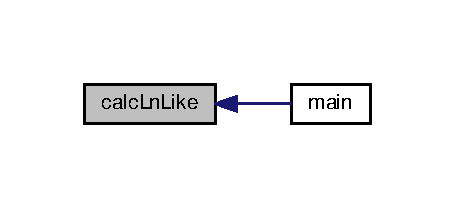
\includegraphics[width=218pt]{_c_a_r_m_a_8hpp_ac6c51cd6959e4a7a5ec0557af951daaa_icgraph}
\end{center}
\end{figure}


\hypertarget{_c_a_r_m_a_8hpp_a9719ae8ef8f4ba7946a78a28412b6273}{\index{C\-A\-R\-M\-A.\-hpp@{C\-A\-R\-M\-A.\-hpp}!calc\-Ln\-Like@{calc\-Ln\-Like}}
\index{calc\-Ln\-Like@{calc\-Ln\-Like}!CARMA.hpp@{C\-A\-R\-M\-A.\-hpp}}
\subsubsection[{calc\-Ln\-Like}]{\setlength{\rightskip}{0pt plus 5cm}double calc\-Ln\-Like (
\begin{DoxyParamCaption}
\item[{double $\ast$}]{walker\-Pos, }
\item[{void $\ast$}]{vd\-Ptr2\-Ln\-Like\-Args}
\end{DoxyParamCaption}
)}}\label{_c_a_r_m_a_8hpp_a9719ae8ef8f4ba7946a78a28412b6273}


Definition at line 208 of file C\-A\-R\-M\-A.\-cpp.

\hypertarget{_c_a_r_m_a_8hpp_a7a7718261954382ab26f32dae64bf3f4}{\index{C\-A\-R\-M\-A.\-hpp@{C\-A\-R\-M\-A.\-hpp}!dtime@{dtime}}
\index{dtime@{dtime}!CARMA.hpp@{C\-A\-R\-M\-A.\-hpp}}
\subsubsection[{dtime}]{\setlength{\rightskip}{0pt plus 5cm}double dtime (
\begin{DoxyParamCaption}
{}
\end{DoxyParamCaption}
)}}\label{_c_a_r_m_a_8hpp_a7a7718261954382ab26f32dae64bf3f4}


Definition at line 318 of file C\-A\-R\-M\-A.\-cpp.



Here is the caller graph for this function\-:\nopagebreak
\begin{figure}[H]
\begin{center}
\leavevmode
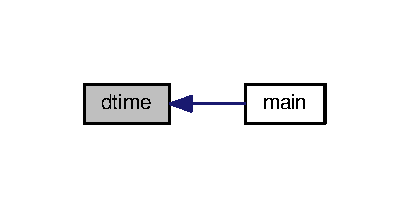
\includegraphics[width=196pt]{_c_a_r_m_a_8hpp_a7a7718261954382ab26f32dae64bf3f4_icgraph}
\end{center}
\end{figure}


\hypertarget{_c_a_r_m_a_8hpp_a0644b006a49b595cc3e4d9cf6dff7303}{\index{C\-A\-R\-M\-A.\-hpp@{C\-A\-R\-M\-A.\-hpp}!kron@{kron}}
\index{kron@{kron}!CARMA.hpp@{C\-A\-R\-M\-A.\-hpp}}
\subsubsection[{kron}]{\setlength{\rightskip}{0pt plus 5cm}void kron (
\begin{DoxyParamCaption}
\item[{int}]{m, }
\item[{int}]{n, }
\item[{double $\ast$}]{A, }
\item[{int}]{p, }
\item[{int}]{q, }
\item[{double $\ast$}]{B, }
\item[{double $\ast$}]{C}
\end{DoxyParamCaption}
)}}\label{_c_a_r_m_a_8hpp_a0644b006a49b595cc3e4d9cf6dff7303}


Definition at line 326 of file C\-A\-R\-M\-A.\-cpp.



Here is the caller graph for this function\-:\nopagebreak
\begin{figure}[H]
\begin{center}
\leavevmode
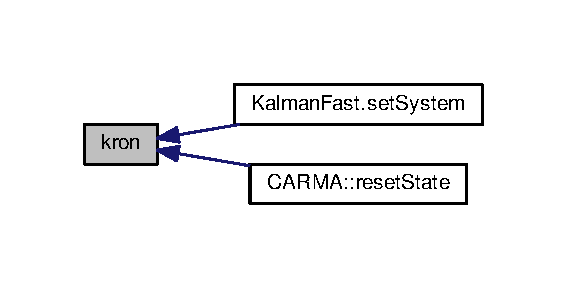
\includegraphics[width=272pt]{_c_a_r_m_a_8hpp_a0644b006a49b595cc3e4d9cf6dff7303_icgraph}
\end{center}
\end{figure}


\hypertarget{_c_a_r_m_a_8hpp_adaf529b8047fb0aa639f2aa494b9cfaf}{\index{C\-A\-R\-M\-A.\-hpp@{C\-A\-R\-M\-A.\-hpp}!view\-Matrix@{view\-Matrix}}
\index{view\-Matrix@{view\-Matrix}!CARMA.hpp@{C\-A\-R\-M\-A.\-hpp}}
\subsubsection[{view\-Matrix}]{\setlength{\rightskip}{0pt plus 5cm}void view\-Matrix (
\begin{DoxyParamCaption}
\item[{int}]{n\-Rows, }
\item[{int}]{n\-Cols, }
\item[{double $\ast$}]{mat}
\end{DoxyParamCaption}
)}}\label{_c_a_r_m_a_8hpp_adaf529b8047fb0aa639f2aa494b9cfaf}


Definition at line 300 of file C\-A\-R\-M\-A.\-cpp.

\hypertarget{_c_a_r_m_a_8hpp_ab43c14961907b75c90cee7b7fd28a3cc}{\index{C\-A\-R\-M\-A.\-hpp@{C\-A\-R\-M\-A.\-hpp}!view\-Matrix@{view\-Matrix}}
\index{view\-Matrix@{view\-Matrix}!CARMA.hpp@{C\-A\-R\-M\-A.\-hpp}}
\subsubsection[{view\-Matrix}]{\setlength{\rightskip}{0pt plus 5cm}void view\-Matrix (
\begin{DoxyParamCaption}
\item[{int}]{n\-Rows, }
\item[{int}]{n\-Cols, }
\item[{complex$<$ double $>$ $\ast$}]{mat}
\end{DoxyParamCaption}
)}}\label{_c_a_r_m_a_8hpp_ab43c14961907b75c90cee7b7fd28a3cc}


Definition at line 309 of file C\-A\-R\-M\-A.\-cpp.

\hypertarget{_c_a_r_m_a_8hpp_a52e65b8de02410a2382d1c0858c43b25}{\index{C\-A\-R\-M\-A.\-hpp@{C\-A\-R\-M\-A.\-hpp}!zero\-Matrix@{zero\-Matrix}}
\index{zero\-Matrix@{zero\-Matrix}!CARMA.hpp@{C\-A\-R\-M\-A.\-hpp}}
\subsubsection[{zero\-Matrix}]{\setlength{\rightskip}{0pt plus 5cm}void zero\-Matrix (
\begin{DoxyParamCaption}
\item[{int}]{n\-Rows, }
\item[{int}]{n\-Cols, }
\item[{int $\ast$}]{mat}
\end{DoxyParamCaption}
)}}\label{_c_a_r_m_a_8hpp_a52e65b8de02410a2382d1c0858c43b25}


Definition at line 268 of file C\-A\-R\-M\-A.\-cpp.

\hypertarget{_c_a_r_m_a_8hpp_ad06e01d494041ea73f3fb05d5208765f}{\index{C\-A\-R\-M\-A.\-hpp@{C\-A\-R\-M\-A.\-hpp}!zero\-Matrix@{zero\-Matrix}}
\index{zero\-Matrix@{zero\-Matrix}!CARMA.hpp@{C\-A\-R\-M\-A.\-hpp}}
\subsubsection[{zero\-Matrix}]{\setlength{\rightskip}{0pt plus 5cm}void zero\-Matrix (
\begin{DoxyParamCaption}
\item[{int}]{n\-Rows, }
\item[{int}]{n\-Cols, }
\item[{lapack\-\_\-int $\ast$}]{mat}
\end{DoxyParamCaption}
)}}\label{_c_a_r_m_a_8hpp_ad06e01d494041ea73f3fb05d5208765f}


Definition at line 276 of file C\-A\-R\-M\-A.\-cpp.

\hypertarget{_c_a_r_m_a_8hpp_acbdde1f5b60f8f09a2561e877f8279e5}{\index{C\-A\-R\-M\-A.\-hpp@{C\-A\-R\-M\-A.\-hpp}!zero\-Matrix@{zero\-Matrix}}
\index{zero\-Matrix@{zero\-Matrix}!CARMA.hpp@{C\-A\-R\-M\-A.\-hpp}}
\subsubsection[{zero\-Matrix}]{\setlength{\rightskip}{0pt plus 5cm}void zero\-Matrix (
\begin{DoxyParamCaption}
\item[{int}]{n\-Rows, }
\item[{int}]{n\-Cols, }
\item[{double $\ast$}]{mat}
\end{DoxyParamCaption}
)}}\label{_c_a_r_m_a_8hpp_acbdde1f5b60f8f09a2561e877f8279e5}


Definition at line 284 of file C\-A\-R\-M\-A.\-cpp.

\hypertarget{_c_a_r_m_a_8hpp_aff867598dfd07c509cec6da77c33fb98}{\index{C\-A\-R\-M\-A.\-hpp@{C\-A\-R\-M\-A.\-hpp}!zero\-Matrix@{zero\-Matrix}}
\index{zero\-Matrix@{zero\-Matrix}!CARMA.hpp@{C\-A\-R\-M\-A.\-hpp}}
\subsubsection[{zero\-Matrix}]{\setlength{\rightskip}{0pt plus 5cm}void zero\-Matrix (
\begin{DoxyParamCaption}
\item[{int}]{n\-Rows, }
\item[{int}]{n\-Cols, }
\item[{complex$<$ double $>$ $\ast$}]{mat}
\end{DoxyParamCaption}
)}}\label{_c_a_r_m_a_8hpp_aff867598dfd07c509cec6da77c33fb98}


Definition at line 292 of file C\-A\-R\-M\-A.\-cpp.


\hypertarget{_constants_8hpp}{\section{/home/vish/code/trunk/cpp/libcarma/cython/include/\-Constants.hpp File Reference}
\label{_constants_8hpp}\index{/home/vish/code/trunk/cpp/libcarma/cython/include/\-Constants.\-hpp@{/home/vish/code/trunk/cpp/libcarma/cython/include/\-Constants.\-hpp}}
}
{\ttfamily \#include $<$complex$>$}\\*
Include dependency graph for Constants.\-hpp\-:
This graph shows which files directly or indirectly include this file\-:
\subsection*{Variables}
\begin{DoxyCompactItemize}
\item 
complex$<$ double $>$ \hyperlink{_constants_8hpp_a1429bd49fdfa9d3e410e025876d72d0e}{complex\-Zero}
\item 
complex$<$ double $>$ \hyperlink{_constants_8hpp_a7fcae12bee2bf97db614c980f2912ded}{complex\-One}
\item 
double \hyperlink{_constants_8hpp_a31c17cc321db72d5ab448b71ea92792f}{pi}
\item 
double \hyperlink{_constants_8hpp_a18bbe41d56bab00212fd0e8e733e9f1f}{pi\-Sq}
\item 
double \hyperlink{_constants_8hpp_ab17e17fb32b792781b807505e7f60c9c}{e}
\item 
double \hyperlink{_constants_8hpp_a5ce1018aef28e71271ae3b4431210720}{infinite\-Val}
\item 
double \hyperlink{_constants_8hpp_a67783a2c4f670ee5a9dadcf428324d32}{G}
\item 
double \hyperlink{_constants_8hpp_a2c09e929a6ea340fc9653cca414b11d3}{c}
\item 
double \hyperlink{_constants_8hpp_a8497a2d27908c87901466c9de72ff8d8}{A\-U}
\item 
double \hyperlink{_constants_8hpp_a2e08042cd1e7eb1861e7115f34fa3acb}{Parsec}
\item 
double \hyperlink{_constants_8hpp_a187ad5035a30f1230f63152e677791ba}{Day}
\item 
double \hyperlink{_constants_8hpp_aa2047f98d2c2eecb4bfe0d2bd43ac10e}{Year}
\item 
double \hyperlink{_constants_8hpp_a81120f2278cac2eb2b1cb85782c83024}{kms2ms}
\item 
double \hyperlink{_constants_8hpp_ada9035453156e0ae346332fde905c274}{Solar\-Mass}
\item 
double \hyperlink{_constants_8hpp_a798a374e513280a7d37661626aab93d5}{Solar\-Mass\-Per\-Cubic\-Parsec}
\item 
double \hyperlink{_constants_8hpp_a6a9e5bbdf108936466078a267b5acd51}{integration\-Time}
\item 
double \hyperlink{_constants_8hpp_abd52f1ed1ece35cffe3fc3e4180ca0f3}{read\-Time}
\item 
int \hyperlink{_constants_8hpp_aeab23e8ce3743c4e554e657ce55c5305}{num\-Integrations\-S\-C}
\item 
int \hyperlink{_constants_8hpp_a045a70c6ff8d3041c66cb29263a0f815}{num\-Integrations\-L\-C}
\item 
double \hyperlink{_constants_8hpp_a3b68866972010d697c2f9e3def43a8c4}{sampling\-Interval\-S\-C}
\item 
double \hyperlink{_constants_8hpp_a7eec0eac1517df1522a3775fc44ddf7d}{sampling\-Interval\-L\-C}
\item 
double \hyperlink{_constants_8hpp_abae737372bcd2caafbf77434f3b0ed97}{sampling\-Frequency\-S\-C}
\item 
double \hyperlink{_constants_8hpp_a102f4d453dc44d0a812bde4a0c8c19c8}{sampling\-Frequency\-L\-C}
\item 
double \hyperlink{_constants_8hpp_a29c58ec25452277c1661f674327a77a4}{Nyquist\-Frequency\-S\-C}
\item 
double \hyperlink{_constants_8hpp_a598be37cc4a0d559305212b7e8c21045}{Nyquist\-Frequency\-L\-C}
\item 
double \hyperlink{_constants_8hpp_ad273a878a46f52a8c720ef7eae03ae4f}{sec\-Per\-Sidereal\-Day}
\item 
double \hyperlink{_constants_8hpp_ad55d7bc1d7b5c686f6197b02498e4eaf}{sc\-Cadence}
\item 
double \hyperlink{_constants_8hpp_ac18142dbc207474c073432f4b28424b9}{lc\-Cadence}
\item 
double \hyperlink{_constants_8hpp_a6a5210c2bcb5149c1073568e5c8d6599}{log2\-Of\-E}
\item 
double \hyperlink{_constants_8hpp_a2b27190acf3cc471e389bb8173544658}{log2\-Pi}
\end{DoxyCompactItemize}


\subsection{Variable Documentation}
\hypertarget{_constants_8hpp_a8497a2d27908c87901466c9de72ff8d8}{\index{Constants.\-hpp@{Constants.\-hpp}!A\-U@{A\-U}}
\index{A\-U@{A\-U}!Constants.hpp@{Constants.\-hpp}}
\subsubsection[{A\-U}]{\setlength{\rightskip}{0pt plus 5cm}double A\-U}}\label{_constants_8hpp_a8497a2d27908c87901466c9de72ff8d8}


Definition at line 27 of file binary\-S\-M\-B\-H\-Demo.\-py.

\hypertarget{_constants_8hpp_a2c09e929a6ea340fc9653cca414b11d3}{\index{Constants.\-hpp@{Constants.\-hpp}!c@{c}}
\index{c@{c}!Constants.hpp@{Constants.\-hpp}}
\subsubsection[{c}]{\setlength{\rightskip}{0pt plus 5cm}double c}}\label{_constants_8hpp_a2c09e929a6ea340fc9653cca414b11d3}


Definition at line 26 of file binary\-S\-M\-B\-H\-Demo.\-py.

\hypertarget{_constants_8hpp_a7fcae12bee2bf97db614c980f2912ded}{\index{Constants.\-hpp@{Constants.\-hpp}!complex\-One@{complex\-One}}
\index{complex\-One@{complex\-One}!Constants.hpp@{Constants.\-hpp}}
\subsubsection[{complex\-One}]{\setlength{\rightskip}{0pt plus 5cm}complex$<$double$>$ complex\-One}}\label{_constants_8hpp_a7fcae12bee2bf97db614c980f2912ded}
\hypertarget{_constants_8hpp_a1429bd49fdfa9d3e410e025876d72d0e}{\index{Constants.\-hpp@{Constants.\-hpp}!complex\-Zero@{complex\-Zero}}
\index{complex\-Zero@{complex\-Zero}!Constants.hpp@{Constants.\-hpp}}
\subsubsection[{complex\-Zero}]{\setlength{\rightskip}{0pt plus 5cm}complex$<$double$>$ complex\-Zero}}\label{_constants_8hpp_a1429bd49fdfa9d3e410e025876d72d0e}
\hypertarget{_constants_8hpp_a187ad5035a30f1230f63152e677791ba}{\index{Constants.\-hpp@{Constants.\-hpp}!Day@{Day}}
\index{Day@{Day}!Constants.hpp@{Constants.\-hpp}}
\subsubsection[{Day}]{\setlength{\rightskip}{0pt plus 5cm}double Day}}\label{_constants_8hpp_a187ad5035a30f1230f63152e677791ba}


Definition at line 30 of file binary\-S\-M\-B\-H\-Demo.\-py.

\hypertarget{_constants_8hpp_ab17e17fb32b792781b807505e7f60c9c}{\index{Constants.\-hpp@{Constants.\-hpp}!e@{e}}
\index{e@{e}!Constants.hpp@{Constants.\-hpp}}
\subsubsection[{e}]{\setlength{\rightskip}{0pt plus 5cm}double e}}\label{_constants_8hpp_ab17e17fb32b792781b807505e7f60c9c}
\hypertarget{_constants_8hpp_a67783a2c4f670ee5a9dadcf428324d32}{\index{Constants.\-hpp@{Constants.\-hpp}!G@{G}}
\index{G@{G}!Constants.hpp@{Constants.\-hpp}}
\subsubsection[{G}]{\setlength{\rightskip}{0pt plus 5cm}double G}}\label{_constants_8hpp_a67783a2c4f670ee5a9dadcf428324d32}


Definition at line 25 of file binary\-S\-M\-B\-H\-Demo.\-py.

\hypertarget{_constants_8hpp_a5ce1018aef28e71271ae3b4431210720}{\index{Constants.\-hpp@{Constants.\-hpp}!infinite\-Val@{infinite\-Val}}
\index{infinite\-Val@{infinite\-Val}!Constants.hpp@{Constants.\-hpp}}
\subsubsection[{infinite\-Val}]{\setlength{\rightskip}{0pt plus 5cm}double infinite\-Val}}\label{_constants_8hpp_a5ce1018aef28e71271ae3b4431210720}
\hypertarget{_constants_8hpp_a6a9e5bbdf108936466078a267b5acd51}{\index{Constants.\-hpp@{Constants.\-hpp}!integration\-Time@{integration\-Time}}
\index{integration\-Time@{integration\-Time}!Constants.hpp@{Constants.\-hpp}}
\subsubsection[{integration\-Time}]{\setlength{\rightskip}{0pt plus 5cm}double integration\-Time}}\label{_constants_8hpp_a6a9e5bbdf108936466078a267b5acd51}
\hypertarget{_constants_8hpp_a81120f2278cac2eb2b1cb85782c83024}{\index{Constants.\-hpp@{Constants.\-hpp}!kms2ms@{kms2ms}}
\index{kms2ms@{kms2ms}!Constants.hpp@{Constants.\-hpp}}
\subsubsection[{kms2ms}]{\setlength{\rightskip}{0pt plus 5cm}double kms2ms}}\label{_constants_8hpp_a81120f2278cac2eb2b1cb85782c83024}


Definition at line 33 of file binary\-S\-M\-B\-H\-Demo.\-py.

\hypertarget{_constants_8hpp_ac18142dbc207474c073432f4b28424b9}{\index{Constants.\-hpp@{Constants.\-hpp}!lc\-Cadence@{lc\-Cadence}}
\index{lc\-Cadence@{lc\-Cadence}!Constants.hpp@{Constants.\-hpp}}
\subsubsection[{lc\-Cadence}]{\setlength{\rightskip}{0pt plus 5cm}double lc\-Cadence}}\label{_constants_8hpp_ac18142dbc207474c073432f4b28424b9}
\hypertarget{_constants_8hpp_a6a5210c2bcb5149c1073568e5c8d6599}{\index{Constants.\-hpp@{Constants.\-hpp}!log2\-Of\-E@{log2\-Of\-E}}
\index{log2\-Of\-E@{log2\-Of\-E}!Constants.hpp@{Constants.\-hpp}}
\subsubsection[{log2\-Of\-E}]{\setlength{\rightskip}{0pt plus 5cm}double log2\-Of\-E}}\label{_constants_8hpp_a6a5210c2bcb5149c1073568e5c8d6599}
\hypertarget{_constants_8hpp_a2b27190acf3cc471e389bb8173544658}{\index{Constants.\-hpp@{Constants.\-hpp}!log2\-Pi@{log2\-Pi}}
\index{log2\-Pi@{log2\-Pi}!Constants.hpp@{Constants.\-hpp}}
\subsubsection[{log2\-Pi}]{\setlength{\rightskip}{0pt plus 5cm}double log2\-Pi}}\label{_constants_8hpp_a2b27190acf3cc471e389bb8173544658}
\hypertarget{_constants_8hpp_a045a70c6ff8d3041c66cb29263a0f815}{\index{Constants.\-hpp@{Constants.\-hpp}!num\-Integrations\-L\-C@{num\-Integrations\-L\-C}}
\index{num\-Integrations\-L\-C@{num\-Integrations\-L\-C}!Constants.hpp@{Constants.\-hpp}}
\subsubsection[{num\-Integrations\-L\-C}]{\setlength{\rightskip}{0pt plus 5cm}int num\-Integrations\-L\-C}}\label{_constants_8hpp_a045a70c6ff8d3041c66cb29263a0f815}
\hypertarget{_constants_8hpp_aeab23e8ce3743c4e554e657ce55c5305}{\index{Constants.\-hpp@{Constants.\-hpp}!num\-Integrations\-S\-C@{num\-Integrations\-S\-C}}
\index{num\-Integrations\-S\-C@{num\-Integrations\-S\-C}!Constants.hpp@{Constants.\-hpp}}
\subsubsection[{num\-Integrations\-S\-C}]{\setlength{\rightskip}{0pt plus 5cm}int num\-Integrations\-S\-C}}\label{_constants_8hpp_aeab23e8ce3743c4e554e657ce55c5305}
\hypertarget{_constants_8hpp_a598be37cc4a0d559305212b7e8c21045}{\index{Constants.\-hpp@{Constants.\-hpp}!Nyquist\-Frequency\-L\-C@{Nyquist\-Frequency\-L\-C}}
\index{Nyquist\-Frequency\-L\-C@{Nyquist\-Frequency\-L\-C}!Constants.hpp@{Constants.\-hpp}}
\subsubsection[{Nyquist\-Frequency\-L\-C}]{\setlength{\rightskip}{0pt plus 5cm}double Nyquist\-Frequency\-L\-C}}\label{_constants_8hpp_a598be37cc4a0d559305212b7e8c21045}
\hypertarget{_constants_8hpp_a29c58ec25452277c1661f674327a77a4}{\index{Constants.\-hpp@{Constants.\-hpp}!Nyquist\-Frequency\-S\-C@{Nyquist\-Frequency\-S\-C}}
\index{Nyquist\-Frequency\-S\-C@{Nyquist\-Frequency\-S\-C}!Constants.hpp@{Constants.\-hpp}}
\subsubsection[{Nyquist\-Frequency\-S\-C}]{\setlength{\rightskip}{0pt plus 5cm}double Nyquist\-Frequency\-S\-C}}\label{_constants_8hpp_a29c58ec25452277c1661f674327a77a4}
\hypertarget{_constants_8hpp_a2e08042cd1e7eb1861e7115f34fa3acb}{\index{Constants.\-hpp@{Constants.\-hpp}!Parsec@{Parsec}}
\index{Parsec@{Parsec}!Constants.hpp@{Constants.\-hpp}}
\subsubsection[{Parsec}]{\setlength{\rightskip}{0pt plus 5cm}double Parsec}}\label{_constants_8hpp_a2e08042cd1e7eb1861e7115f34fa3acb}


Definition at line 28 of file binary\-S\-M\-B\-H\-Demo.\-py.

\hypertarget{_constants_8hpp_a31c17cc321db72d5ab448b71ea92792f}{\index{Constants.\-hpp@{Constants.\-hpp}!pi@{pi}}
\index{pi@{pi}!Constants.hpp@{Constants.\-hpp}}
\subsubsection[{pi}]{\setlength{\rightskip}{0pt plus 5cm}double pi}}\label{_constants_8hpp_a31c17cc321db72d5ab448b71ea92792f}
\hypertarget{_constants_8hpp_a18bbe41d56bab00212fd0e8e733e9f1f}{\index{Constants.\-hpp@{Constants.\-hpp}!pi\-Sq@{pi\-Sq}}
\index{pi\-Sq@{pi\-Sq}!Constants.hpp@{Constants.\-hpp}}
\subsubsection[{pi\-Sq}]{\setlength{\rightskip}{0pt plus 5cm}double pi\-Sq}}\label{_constants_8hpp_a18bbe41d56bab00212fd0e8e733e9f1f}
\hypertarget{_constants_8hpp_abd52f1ed1ece35cffe3fc3e4180ca0f3}{\index{Constants.\-hpp@{Constants.\-hpp}!read\-Time@{read\-Time}}
\index{read\-Time@{read\-Time}!Constants.hpp@{Constants.\-hpp}}
\subsubsection[{read\-Time}]{\setlength{\rightskip}{0pt plus 5cm}double read\-Time}}\label{_constants_8hpp_abd52f1ed1ece35cffe3fc3e4180ca0f3}
\hypertarget{_constants_8hpp_a102f4d453dc44d0a812bde4a0c8c19c8}{\index{Constants.\-hpp@{Constants.\-hpp}!sampling\-Frequency\-L\-C@{sampling\-Frequency\-L\-C}}
\index{sampling\-Frequency\-L\-C@{sampling\-Frequency\-L\-C}!Constants.hpp@{Constants.\-hpp}}
\subsubsection[{sampling\-Frequency\-L\-C}]{\setlength{\rightskip}{0pt plus 5cm}double sampling\-Frequency\-L\-C}}\label{_constants_8hpp_a102f4d453dc44d0a812bde4a0c8c19c8}
\hypertarget{_constants_8hpp_abae737372bcd2caafbf77434f3b0ed97}{\index{Constants.\-hpp@{Constants.\-hpp}!sampling\-Frequency\-S\-C@{sampling\-Frequency\-S\-C}}
\index{sampling\-Frequency\-S\-C@{sampling\-Frequency\-S\-C}!Constants.hpp@{Constants.\-hpp}}
\subsubsection[{sampling\-Frequency\-S\-C}]{\setlength{\rightskip}{0pt plus 5cm}double sampling\-Frequency\-S\-C}}\label{_constants_8hpp_abae737372bcd2caafbf77434f3b0ed97}
\hypertarget{_constants_8hpp_a7eec0eac1517df1522a3775fc44ddf7d}{\index{Constants.\-hpp@{Constants.\-hpp}!sampling\-Interval\-L\-C@{sampling\-Interval\-L\-C}}
\index{sampling\-Interval\-L\-C@{sampling\-Interval\-L\-C}!Constants.hpp@{Constants.\-hpp}}
\subsubsection[{sampling\-Interval\-L\-C}]{\setlength{\rightskip}{0pt plus 5cm}double sampling\-Interval\-L\-C}}\label{_constants_8hpp_a7eec0eac1517df1522a3775fc44ddf7d}
\hypertarget{_constants_8hpp_a3b68866972010d697c2f9e3def43a8c4}{\index{Constants.\-hpp@{Constants.\-hpp}!sampling\-Interval\-S\-C@{sampling\-Interval\-S\-C}}
\index{sampling\-Interval\-S\-C@{sampling\-Interval\-S\-C}!Constants.hpp@{Constants.\-hpp}}
\subsubsection[{sampling\-Interval\-S\-C}]{\setlength{\rightskip}{0pt plus 5cm}double sampling\-Interval\-S\-C}}\label{_constants_8hpp_a3b68866972010d697c2f9e3def43a8c4}
\hypertarget{_constants_8hpp_ad55d7bc1d7b5c686f6197b02498e4eaf}{\index{Constants.\-hpp@{Constants.\-hpp}!sc\-Cadence@{sc\-Cadence}}
\index{sc\-Cadence@{sc\-Cadence}!Constants.hpp@{Constants.\-hpp}}
\subsubsection[{sc\-Cadence}]{\setlength{\rightskip}{0pt plus 5cm}double sc\-Cadence}}\label{_constants_8hpp_ad55d7bc1d7b5c686f6197b02498e4eaf}
\hypertarget{_constants_8hpp_ad273a878a46f52a8c720ef7eae03ae4f}{\index{Constants.\-hpp@{Constants.\-hpp}!sec\-Per\-Sidereal\-Day@{sec\-Per\-Sidereal\-Day}}
\index{sec\-Per\-Sidereal\-Day@{sec\-Per\-Sidereal\-Day}!Constants.hpp@{Constants.\-hpp}}
\subsubsection[{sec\-Per\-Sidereal\-Day}]{\setlength{\rightskip}{0pt plus 5cm}double sec\-Per\-Sidereal\-Day}}\label{_constants_8hpp_ad273a878a46f52a8c720ef7eae03ae4f}
\hypertarget{_constants_8hpp_ada9035453156e0ae346332fde905c274}{\index{Constants.\-hpp@{Constants.\-hpp}!Solar\-Mass@{Solar\-Mass}}
\index{Solar\-Mass@{Solar\-Mass}!Constants.hpp@{Constants.\-hpp}}
\subsubsection[{Solar\-Mass}]{\setlength{\rightskip}{0pt plus 5cm}double Solar\-Mass}}\label{_constants_8hpp_ada9035453156e0ae346332fde905c274}


Definition at line 32 of file binary\-S\-M\-B\-H\-Demo.\-py.

\hypertarget{_constants_8hpp_a798a374e513280a7d37661626aab93d5}{\index{Constants.\-hpp@{Constants.\-hpp}!Solar\-Mass\-Per\-Cubic\-Parsec@{Solar\-Mass\-Per\-Cubic\-Parsec}}
\index{Solar\-Mass\-Per\-Cubic\-Parsec@{Solar\-Mass\-Per\-Cubic\-Parsec}!Constants.hpp@{Constants.\-hpp}}
\subsubsection[{Solar\-Mass\-Per\-Cubic\-Parsec}]{\setlength{\rightskip}{0pt plus 5cm}double Solar\-Mass\-Per\-Cubic\-Parsec}}\label{_constants_8hpp_a798a374e513280a7d37661626aab93d5}


Definition at line 34 of file binary\-S\-M\-B\-H\-Demo.\-py.

\hypertarget{_constants_8hpp_aa2047f98d2c2eecb4bfe0d2bd43ac10e}{\index{Constants.\-hpp@{Constants.\-hpp}!Year@{Year}}
\index{Year@{Year}!Constants.hpp@{Constants.\-hpp}}
\subsubsection[{Year}]{\setlength{\rightskip}{0pt plus 5cm}double Year}}\label{_constants_8hpp_aa2047f98d2c2eecb4bfe0d2bd43ac10e}


Definition at line 29 of file binary\-S\-M\-B\-H\-Demo.\-py.


\hypertarget{_correlation_8hpp}{\section{/home/vish/code/trunk/cpp/libcarma/include/\-Correlation.hpp File Reference}
\label{_correlation_8hpp}\index{/home/vish/code/trunk/cpp/libcarma/include/\-Correlation.\-hpp@{/home/vish/code/trunk/cpp/libcarma/include/\-Correlation.\-hpp}}
}
{\ttfamily \#include $<$mkl.\-h$>$}\\*
{\ttfamily \#include $<$mkl\-\_\-types.\-h$>$}\\*
Include dependency graph for Correlation.\-hpp\-:\nopagebreak
\begin{figure}[H]
\begin{center}
\leavevmode
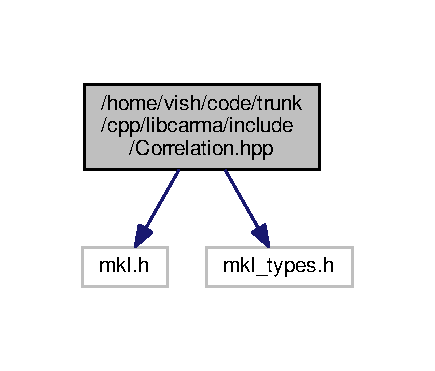
\includegraphics[width=209pt]{_correlation_8hpp__incl}
\end{center}
\end{figure}
This graph shows which files directly or indirectly include this file\-:\nopagebreak
\begin{figure}[H]
\begin{center}
\leavevmode
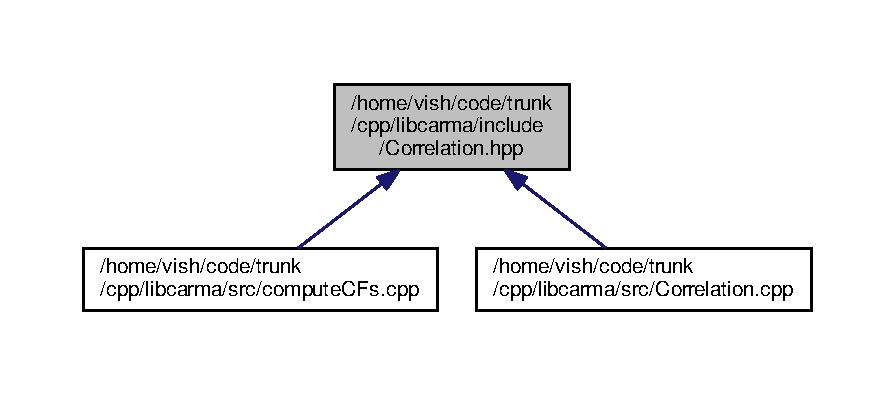
\includegraphics[width=350pt]{_correlation_8hpp__dep__incl}
\end{center}
\end{figure}
\subsection*{Functions}
\begin{DoxyCompactItemize}
\item 
void \hyperlink{_correlation_8hpp_adaf529b8047fb0aa639f2aa494b9cfaf}{view\-Matrix} (int n\-Rows, int n\-Cols, double $\ast$mat)
\item 
double \hyperlink{_correlation_8hpp_a7a7718261954382ab26f32dae64bf3f4}{dtime} ()
\item 
void \hyperlink{_correlation_8hpp_ab5d562f3b6a902b3dcabe4fcebf9f581}{A\-C\-V\-F} (int num\-Cadences, const double $\ast$const y, const double $\ast$const mask, double $\ast$acvf)
\item 
void \hyperlink{_correlation_8hpp_a0733d619e610b9c1d5949f8a93e7af50}{A\-C\-F} (int num\-Cadences, const double $\ast$const acvf, double $\ast$acf)
\item 
void \hyperlink{_correlation_8hpp_aa90de21932497f2965056021a30149b7}{P\-A\-C\-F} (int num\-Cadences, int max\-Lag, const double $\ast$const acvf, double $\ast$pacf)
\item 
void \hyperlink{_correlation_8hpp_abf87d03b9b305f4e43dc5c20da98c7a2}{S\-F1} (int num\-Cadences, const double $\ast$const acvf, double $\ast$sf1)
\end{DoxyCompactItemize}


\subsection{Function Documentation}
\hypertarget{_correlation_8hpp_a0733d619e610b9c1d5949f8a93e7af50}{\index{Correlation.\-hpp@{Correlation.\-hpp}!A\-C\-F@{A\-C\-F}}
\index{A\-C\-F@{A\-C\-F}!Correlation.hpp@{Correlation.\-hpp}}
\subsubsection[{A\-C\-F}]{\setlength{\rightskip}{0pt plus 5cm}void A\-C\-F (
\begin{DoxyParamCaption}
\item[{int}]{num\-Cadences, }
\item[{const double $\ast$const}]{acvf, }
\item[{double $\ast$}]{acf}
\end{DoxyParamCaption}
)}}\label{_correlation_8hpp_a0733d619e610b9c1d5949f8a93e7af50}


Definition at line 61 of file Correlation.\-cpp.



Here is the caller graph for this function\-:\nopagebreak
\begin{figure}[H]
\begin{center}
\leavevmode
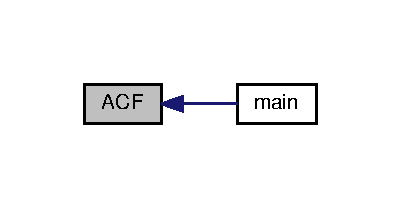
\includegraphics[width=192pt]{_correlation_8hpp_a0733d619e610b9c1d5949f8a93e7af50_icgraph}
\end{center}
\end{figure}


\hypertarget{_correlation_8hpp_ab5d562f3b6a902b3dcabe4fcebf9f581}{\index{Correlation.\-hpp@{Correlation.\-hpp}!A\-C\-V\-F@{A\-C\-V\-F}}
\index{A\-C\-V\-F@{A\-C\-V\-F}!Correlation.hpp@{Correlation.\-hpp}}
\subsubsection[{A\-C\-V\-F}]{\setlength{\rightskip}{0pt plus 5cm}void A\-C\-V\-F (
\begin{DoxyParamCaption}
\item[{int}]{num\-Cadences, }
\item[{const double $\ast$const}]{y, }
\item[{const double $\ast$const}]{mask, }
\item[{double $\ast$}]{acvf}
\end{DoxyParamCaption}
)}}\label{_correlation_8hpp_ab5d562f3b6a902b3dcabe4fcebf9f581}
First remove the mean.

Now, following \char`\"{}\-Spectrum Estimation with Missing Observations\char`\"{} by Richard H. Jones (Rcvd 1969, Rvsd 1971) we compute for each lag.

Following \char`\"{}\-Modern Applied Statistics with S\char`\"{} by W.\-N. Venables \& B.\-D. Ripley (4th Ed, 1992) we compute for each lag. 

Definition at line 18 of file Correlation.\-cpp.



Here is the caller graph for this function\-:\nopagebreak
\begin{figure}[H]
\begin{center}
\leavevmode
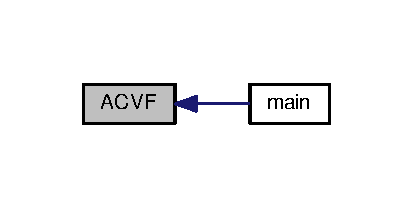
\includegraphics[width=198pt]{_correlation_8hpp_ab5d562f3b6a902b3dcabe4fcebf9f581_icgraph}
\end{center}
\end{figure}


\hypertarget{_correlation_8hpp_a7a7718261954382ab26f32dae64bf3f4}{\index{Correlation.\-hpp@{Correlation.\-hpp}!dtime@{dtime}}
\index{dtime@{dtime}!Correlation.hpp@{Correlation.\-hpp}}
\subsubsection[{dtime}]{\setlength{\rightskip}{0pt plus 5cm}double dtime (
\begin{DoxyParamCaption}
{}
\end{DoxyParamCaption}
)}}\label{_correlation_8hpp_a7a7718261954382ab26f32dae64bf3f4}


Definition at line 318 of file C\-A\-R\-M\-A.\-cpp.

\hypertarget{_correlation_8hpp_aa90de21932497f2965056021a30149b7}{\index{Correlation.\-hpp@{Correlation.\-hpp}!P\-A\-C\-F@{P\-A\-C\-F}}
\index{P\-A\-C\-F@{P\-A\-C\-F}!Correlation.hpp@{Correlation.\-hpp}}
\subsubsection[{P\-A\-C\-F}]{\setlength{\rightskip}{0pt plus 5cm}void P\-A\-C\-F (
\begin{DoxyParamCaption}
\item[{int}]{num\-Cadences, }
\item[{int}]{max\-Lag, }
\item[{const double $\ast$const}]{acvf, }
\item[{double $\ast$}]{pacf}
\end{DoxyParamCaption}
)}}\label{_correlation_8hpp_aa90de21932497f2965056021a30149b7}


Definition at line 70 of file Correlation.\-cpp.



Here is the call graph for this function\-:\nopagebreak
\begin{figure}[H]
\begin{center}
\leavevmode
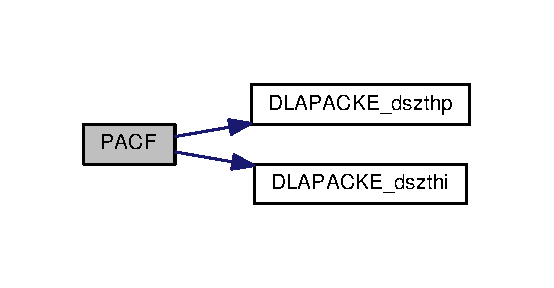
\includegraphics[width=266pt]{_correlation_8hpp_aa90de21932497f2965056021a30149b7_cgraph}
\end{center}
\end{figure}




Here is the caller graph for this function\-:\nopagebreak
\begin{figure}[H]
\begin{center}
\leavevmode
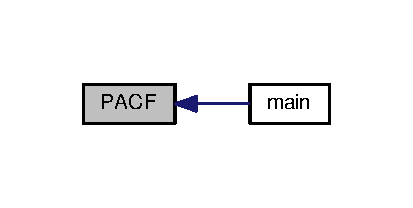
\includegraphics[width=198pt]{_correlation_8hpp_aa90de21932497f2965056021a30149b7_icgraph}
\end{center}
\end{figure}


\hypertarget{_correlation_8hpp_abf87d03b9b305f4e43dc5c20da98c7a2}{\index{Correlation.\-hpp@{Correlation.\-hpp}!S\-F1@{S\-F1}}
\index{S\-F1@{S\-F1}!Correlation.hpp@{Correlation.\-hpp}}
\subsubsection[{S\-F1}]{\setlength{\rightskip}{0pt plus 5cm}void S\-F1 (
\begin{DoxyParamCaption}
\item[{int}]{num\-Cadences, }
\item[{const double $\ast$const}]{acvf, }
\item[{double $\ast$}]{sf1}
\end{DoxyParamCaption}
)}}\label{_correlation_8hpp_abf87d03b9b305f4e43dc5c20da98c7a2}


Definition at line 127 of file Correlation.\-cpp.



Here is the caller graph for this function\-:\nopagebreak
\begin{figure}[H]
\begin{center}
\leavevmode
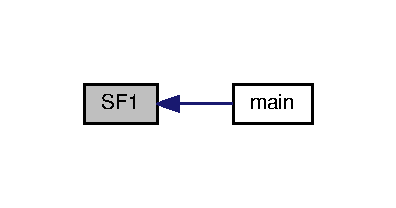
\includegraphics[width=190pt]{_correlation_8hpp_abf87d03b9b305f4e43dc5c20da98c7a2_icgraph}
\end{center}
\end{figure}


\hypertarget{_correlation_8hpp_adaf529b8047fb0aa639f2aa494b9cfaf}{\index{Correlation.\-hpp@{Correlation.\-hpp}!view\-Matrix@{view\-Matrix}}
\index{view\-Matrix@{view\-Matrix}!Correlation.hpp@{Correlation.\-hpp}}
\subsubsection[{view\-Matrix}]{\setlength{\rightskip}{0pt plus 5cm}void view\-Matrix (
\begin{DoxyParamCaption}
\item[{int}]{n\-Rows, }
\item[{int}]{n\-Cols, }
\item[{double $\ast$}]{mat}
\end{DoxyParamCaption}
)}}\label{_correlation_8hpp_adaf529b8047fb0aa639f2aa494b9cfaf}


Definition at line 300 of file C\-A\-R\-M\-A.\-cpp.



Here is the caller graph for this function\-:\nopagebreak
\begin{figure}[H]
\begin{center}
\leavevmode
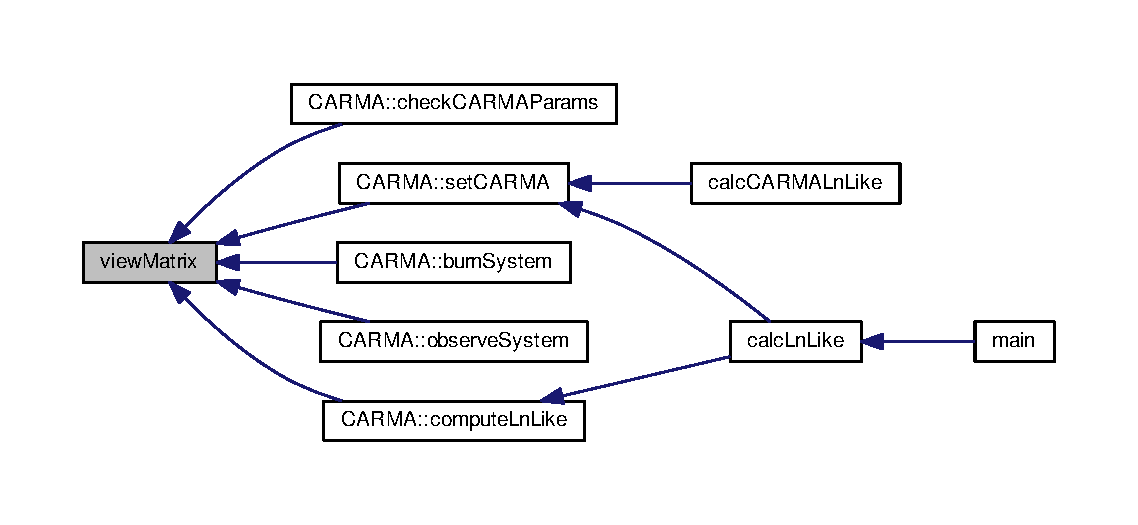
\includegraphics[width=336pt]{_correlation_8hpp_adaf529b8047fb0aa639f2aa494b9cfaf_icgraph}
\end{center}
\end{figure}



\hypertarget{_d_l_a_p_a_c_k_e_8hpp}{\section{/home/vish/code/trunk/cpp/libcarma/include/\-D\-L\-A\-P\-A\-C\-K\-E.hpp File Reference}
\label{_d_l_a_p_a_c_k_e_8hpp}\index{/home/vish/code/trunk/cpp/libcarma/include/\-D\-L\-A\-P\-A\-C\-K\-E.\-hpp@{/home/vish/code/trunk/cpp/libcarma/include/\-D\-L\-A\-P\-A\-C\-K\-E.\-hpp}}
}
This graph shows which files directly or indirectly include this file\-:\nopagebreak
\begin{figure}[H]
\begin{center}
\leavevmode
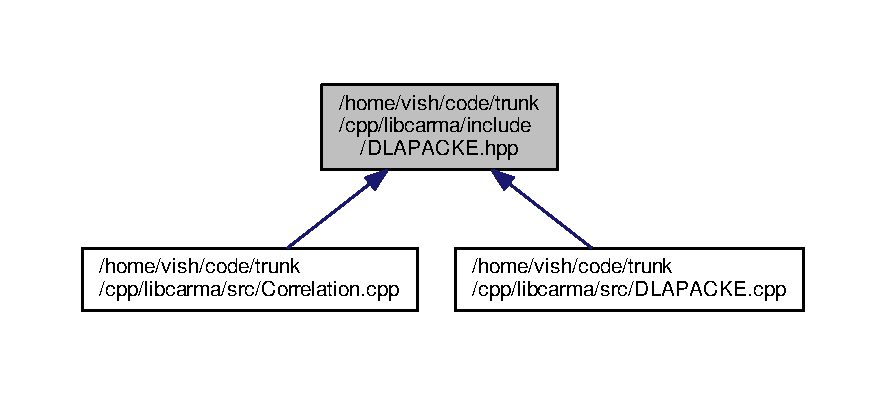
\includegraphics[width=350pt]{_d_l_a_p_a_c_k_e_8hpp__dep__incl}
\end{center}
\end{figure}
\subsection*{Functions}
\begin{DoxyCompactItemize}
\item 
double \hyperlink{_d_l_a_p_a_c_k_e_8hpp_ab3a159d8cd9adbd800461142e5a092a1}{D\-L\-A\-P\-A\-C\-K\-E\-\_\-dgzthp} (int N, double $\ast$R, double $\ast$X, double $\ast$Y)
\item 
double \hyperlink{_d_l_a_p_a_c_k_e_8hpp_a5809c14c7f2e31b2aed7ca2bd8866d97}{D\-L\-A\-P\-A\-C\-K\-E\-\_\-dgzthi} (int i, int j, int N, double $\ast$X)
\item 
double \hyperlink{_d_l_a_p_a_c_k_e_8hpp_a88327457c7fd42b447d9b51cfb77a658}{D\-L\-A\-P\-A\-C\-K\-E\-\_\-dszthp} (int N, double $\ast$R, double $\ast$X, double $\ast$Y)
\item 
double \hyperlink{_d_l_a_p_a_c_k_e_8hpp_a03ec6e9bacb5d503a156b210eab66db5}{D\-L\-A\-P\-A\-C\-K\-E\-\_\-dszthi} (int i, int j, int N, double $\ast$X)
\end{DoxyCompactItemize}


\subsection{Function Documentation}
\hypertarget{_d_l_a_p_a_c_k_e_8hpp_a5809c14c7f2e31b2aed7ca2bd8866d97}{\index{D\-L\-A\-P\-A\-C\-K\-E.\-hpp@{D\-L\-A\-P\-A\-C\-K\-E.\-hpp}!D\-L\-A\-P\-A\-C\-K\-E\-\_\-dgzthi@{D\-L\-A\-P\-A\-C\-K\-E\-\_\-dgzthi}}
\index{D\-L\-A\-P\-A\-C\-K\-E\-\_\-dgzthi@{D\-L\-A\-P\-A\-C\-K\-E\-\_\-dgzthi}!DLAPACKE.hpp@{D\-L\-A\-P\-A\-C\-K\-E.\-hpp}}
\subsubsection[{D\-L\-A\-P\-A\-C\-K\-E\-\_\-dgzthi}]{\setlength{\rightskip}{0pt plus 5cm}double D\-L\-A\-P\-A\-C\-K\-E\-\_\-dgzthi (
\begin{DoxyParamCaption}
\item[{int}]{i, }
\item[{int}]{j, }
\item[{int}]{N, }
\item[{double $\ast$}]{X}
\end{DoxyParamCaption}
)}}\label{_d_l_a_p_a_c_k_e_8hpp_a5809c14c7f2e31b2aed7ca2bd8866d97}


Definition at line 43 of file D\-L\-A\-P\-A\-C\-K\-E.\-cpp.

\hypertarget{_d_l_a_p_a_c_k_e_8hpp_ab3a159d8cd9adbd800461142e5a092a1}{\index{D\-L\-A\-P\-A\-C\-K\-E.\-hpp@{D\-L\-A\-P\-A\-C\-K\-E.\-hpp}!D\-L\-A\-P\-A\-C\-K\-E\-\_\-dgzthp@{D\-L\-A\-P\-A\-C\-K\-E\-\_\-dgzthp}}
\index{D\-L\-A\-P\-A\-C\-K\-E\-\_\-dgzthp@{D\-L\-A\-P\-A\-C\-K\-E\-\_\-dgzthp}!DLAPACKE.hpp@{D\-L\-A\-P\-A\-C\-K\-E.\-hpp}}
\subsubsection[{D\-L\-A\-P\-A\-C\-K\-E\-\_\-dgzthp}]{\setlength{\rightskip}{0pt plus 5cm}double D\-L\-A\-P\-A\-C\-K\-E\-\_\-dgzthp (
\begin{DoxyParamCaption}
\item[{int}]{N, }
\item[{double $\ast$}]{R, }
\item[{double $\ast$}]{X, }
\item[{double $\ast$}]{Y}
\end{DoxyParamCaption}
)}}\label{_d_l_a_p_a_c_k_e_8hpp_ab3a159d8cd9adbd800461142e5a092a1}


Definition at line 11 of file D\-L\-A\-P\-A\-C\-K\-E.\-cpp.

\hypertarget{_d_l_a_p_a_c_k_e_8hpp_a03ec6e9bacb5d503a156b210eab66db5}{\index{D\-L\-A\-P\-A\-C\-K\-E.\-hpp@{D\-L\-A\-P\-A\-C\-K\-E.\-hpp}!D\-L\-A\-P\-A\-C\-K\-E\-\_\-dszthi@{D\-L\-A\-P\-A\-C\-K\-E\-\_\-dszthi}}
\index{D\-L\-A\-P\-A\-C\-K\-E\-\_\-dszthi@{D\-L\-A\-P\-A\-C\-K\-E\-\_\-dszthi}!DLAPACKE.hpp@{D\-L\-A\-P\-A\-C\-K\-E.\-hpp}}
\subsubsection[{D\-L\-A\-P\-A\-C\-K\-E\-\_\-dszthi}]{\setlength{\rightskip}{0pt plus 5cm}double D\-L\-A\-P\-A\-C\-K\-E\-\_\-dszthi (
\begin{DoxyParamCaption}
\item[{int}]{i, }
\item[{int}]{j, }
\item[{int}]{N, }
\item[{double $\ast$}]{X}
\end{DoxyParamCaption}
)}}\label{_d_l_a_p_a_c_k_e_8hpp_a03ec6e9bacb5d503a156b210eab66db5}


Definition at line 112 of file D\-L\-A\-P\-A\-C\-K\-E.\-cpp.



Here is the caller graph for this function\-:\nopagebreak
\begin{figure}[H]
\begin{center}
\leavevmode
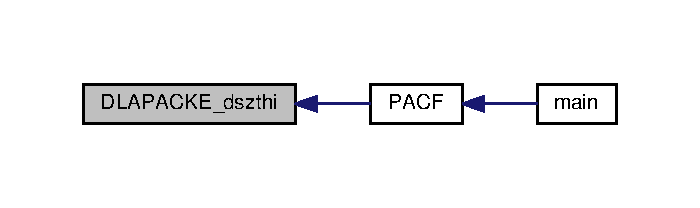
\includegraphics[width=336pt]{_d_l_a_p_a_c_k_e_8hpp_a03ec6e9bacb5d503a156b210eab66db5_icgraph}
\end{center}
\end{figure}


\hypertarget{_d_l_a_p_a_c_k_e_8hpp_a88327457c7fd42b447d9b51cfb77a658}{\index{D\-L\-A\-P\-A\-C\-K\-E.\-hpp@{D\-L\-A\-P\-A\-C\-K\-E.\-hpp}!D\-L\-A\-P\-A\-C\-K\-E\-\_\-dszthp@{D\-L\-A\-P\-A\-C\-K\-E\-\_\-dszthp}}
\index{D\-L\-A\-P\-A\-C\-K\-E\-\_\-dszthp@{D\-L\-A\-P\-A\-C\-K\-E\-\_\-dszthp}!DLAPACKE.hpp@{D\-L\-A\-P\-A\-C\-K\-E.\-hpp}}
\subsubsection[{D\-L\-A\-P\-A\-C\-K\-E\-\_\-dszthp}]{\setlength{\rightskip}{0pt plus 5cm}double D\-L\-A\-P\-A\-C\-K\-E\-\_\-dszthp (
\begin{DoxyParamCaption}
\item[{int}]{N, }
\item[{double $\ast$}]{R, }
\item[{double $\ast$}]{X, }
\item[{double $\ast$}]{Y}
\end{DoxyParamCaption}
)}}\label{_d_l_a_p_a_c_k_e_8hpp_a88327457c7fd42b447d9b51cfb77a658}


Definition at line 87 of file D\-L\-A\-P\-A\-C\-K\-E.\-cpp.



Here is the caller graph for this function\-:\nopagebreak
\begin{figure}[H]
\begin{center}
\leavevmode
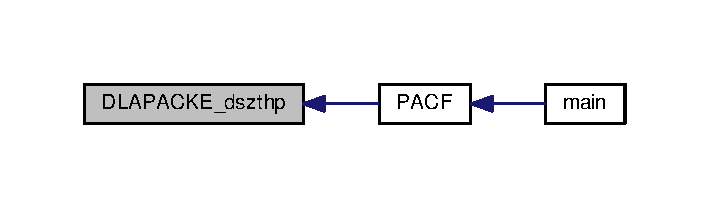
\includegraphics[width=340pt]{_d_l_a_p_a_c_k_e_8hpp_a88327457c7fd42b447d9b51cfb77a658_icgraph}
\end{center}
\end{figure}



\hypertarget{_gauss_m_v_8hpp}{\section{/home/vish/code/trunk/cpp/libcarma/include/\-Gauss\-M\-V.hpp File Reference}
\label{_gauss_m_v_8hpp}\index{/home/vish/code/trunk/cpp/libcarma/include/\-Gauss\-M\-V.\-hpp@{/home/vish/code/trunk/cpp/libcarma/include/\-Gauss\-M\-V.\-hpp}}
}
{\ttfamily \#include $<$mkl.\-h$>$}\\*
{\ttfamily \#include $<$mkl\-\_\-types.\-h$>$}\\*
Include dependency graph for Gauss\-M\-V.\-hpp\-:\nopagebreak
\begin{figure}[H]
\begin{center}
\leavevmode
\includegraphics[width=209pt]{_gauss_m_v_8hpp__incl}
\end{center}
\end{figure}
This graph shows which files directly or indirectly include this file\-:\nopagebreak
\begin{figure}[H]
\begin{center}
\leavevmode
\includegraphics[width=236pt]{_gauss_m_v_8hpp__dep__incl}
\end{center}
\end{figure}
\subsection*{Classes}
\begin{DoxyCompactItemize}
\item 
struct \hyperlink{struct_gauss_m_v}{Gauss\-M\-V}
\item 
struct \hyperlink{struct_ln_like_args}{Ln\-Like\-Args}
\end{DoxyCompactItemize}
\subsection*{Functions}
\begin{DoxyCompactItemize}
\item 
double \hyperlink{_gauss_m_v_8hpp_a9719ae8ef8f4ba7946a78a28412b6273}{calc\-Ln\-Like} (double $\ast$walker\-Pos, void $\ast$vd\-Ptr2\-Ln\-Like\-Args)
\end{DoxyCompactItemize}


\subsection{Function Documentation}
\hypertarget{_gauss_m_v_8hpp_a9719ae8ef8f4ba7946a78a28412b6273}{\index{Gauss\-M\-V.\-hpp@{Gauss\-M\-V.\-hpp}!calc\-Ln\-Like@{calc\-Ln\-Like}}
\index{calc\-Ln\-Like@{calc\-Ln\-Like}!GaussMV.hpp@{Gauss\-M\-V.\-hpp}}
\subsubsection[{calc\-Ln\-Like}]{\setlength{\rightskip}{0pt plus 5cm}double calc\-Ln\-Like (
\begin{DoxyParamCaption}
\item[{double $\ast$}]{walker\-Pos, }
\item[{void $\ast$}]{vd\-Ptr2\-Ln\-Like\-Args}
\end{DoxyParamCaption}
)}}\label{_gauss_m_v_8hpp_a9719ae8ef8f4ba7946a78a28412b6273}


Definition at line 208 of file C\-A\-R\-M\-A.\-cpp.


\hypertarget{_kepler_8hpp}{\section{/home/vish/code/trunk/cpp/libcarma/include/\-Kepler.hpp File Reference}
\label{_kepler_8hpp}\index{/home/vish/code/trunk/cpp/libcarma/include/\-Kepler.\-hpp@{/home/vish/code/trunk/cpp/libcarma/include/\-Kepler.\-hpp}}
}
{\ttfamily \#include \char`\"{}Constants.\-hpp\char`\"{}}\\*
{\ttfamily \#include \char`\"{}Spherical.\-hpp\char`\"{}}\\*
{\ttfamily \#include \char`\"{}Obj.\-hpp\char`\"{}}\\*
Include dependency graph for Kepler.\-hpp\-:\nopagebreak
\begin{figure}[H]
\begin{center}
\leavevmode
\includegraphics[width=261pt]{_kepler_8hpp__incl}
\end{center}
\end{figure}
This graph shows which files directly or indirectly include this file\-:\nopagebreak
\begin{figure}[H]
\begin{center}
\leavevmode
\includegraphics[width=350pt]{_kepler_8hpp__dep__incl}
\end{center}
\end{figure}
\subsection*{Classes}
\begin{DoxyCompactItemize}
\item 
class \hyperlink{class_kepler_obj}{Kepler\-Obj}
\end{DoxyCompactItemize}
\subsection*{Functions}
\begin{DoxyCompactItemize}
\item 
bool \hyperlink{_kepler_8hpp_ad5f452781f97494e147976dc434e47c6}{compare\-S\-F1} (const array$<$ double, 2 $>$ \&a, const array$<$ double, 2 $>$ \&b)
\end{DoxyCompactItemize}


\subsection{Function Documentation}
\hypertarget{_kepler_8hpp_ad5f452781f97494e147976dc434e47c6}{\index{Kepler.\-hpp@{Kepler.\-hpp}!compare\-S\-F1@{compare\-S\-F1}}
\index{compare\-S\-F1@{compare\-S\-F1}!Kepler.hpp@{Kepler.\-hpp}}
\subsubsection[{compare\-S\-F1}]{\setlength{\rightskip}{0pt plus 5cm}bool compare\-S\-F1 (
\begin{DoxyParamCaption}
\item[{const array$<$ double, 2 $>$ \&}]{a, }
\item[{const array$<$ double, 2 $>$ \&}]{b}
\end{DoxyParamCaption}
)}}\label{_kepler_8hpp_ad5f452781f97494e147976dc434e47c6}


Definition at line 852 of file Kepler.\-cpp.


\hypertarget{_m_c_m_c_8hpp}{\section{/home/vish/code/trunk/cpp/libcarma/cython/include/\-M\-C\-M\-C.hpp File Reference}
\label{_m_c_m_c_8hpp}\index{/home/vish/code/trunk/cpp/libcarma/cython/include/\-M\-C\-M\-C.\-hpp@{/home/vish/code/trunk/cpp/libcarma/cython/include/\-M\-C\-M\-C.\-hpp}}
}
This graph shows which files directly or indirectly include this file\-:
\subsection*{Classes}
\begin{DoxyCompactItemize}
\item 
class \hyperlink{class_ensemble_sampler}{Ensemble\-Sampler}
\end{DoxyCompactItemize}

\hypertarget{_obj_8hpp}{\section{/home/vish/code/trunk/cpp/libcarma/include/\-Obj.hpp File Reference}
\label{_obj_8hpp}\index{/home/vish/code/trunk/cpp/libcarma/include/\-Obj.\-hpp@{/home/vish/code/trunk/cpp/libcarma/include/\-Obj.\-hpp}}
}
{\ttfamily \#include \char`\"{}Universe.\-hpp\char`\"{}}\\*
{\ttfamily \#include \char`\"{}Spherical.\-hpp\char`\"{}}\\*
Include dependency graph for Obj.\-hpp\-:\nopagebreak
\begin{figure}[H]
\begin{center}
\leavevmode
\includegraphics[width=252pt]{_obj_8hpp__incl}
\end{center}
\end{figure}
This graph shows which files directly or indirectly include this file\-:\nopagebreak
\begin{figure}[H]
\begin{center}
\leavevmode
\includegraphics[width=350pt]{_obj_8hpp__dep__incl}
\end{center}
\end{figure}
\subsection*{Classes}
\begin{DoxyCompactItemize}
\item 
class \hyperlink{class_obj}{Obj}
\end{DoxyCompactItemize}

\hypertarget{_spherical_8hpp}{\section{/home/vish/code/trunk/cpp/libcarma/include/\-Spherical.hpp File Reference}
\label{_spherical_8hpp}\index{/home/vish/code/trunk/cpp/libcarma/include/\-Spherical.\-hpp@{/home/vish/code/trunk/cpp/libcarma/include/\-Spherical.\-hpp}}
}
{\ttfamily \#include \char`\"{}Constants.\-hpp\char`\"{}}\\*
{\ttfamily \#include \char`\"{}Universe.\-hpp\char`\"{}}\\*
Include dependency graph for Spherical.\-hpp\-:\nopagebreak
\begin{figure}[H]
\begin{center}
\leavevmode
\includegraphics[width=252pt]{_spherical_8hpp__incl}
\end{center}
\end{figure}
This graph shows which files directly or indirectly include this file\-:\nopagebreak
\begin{figure}[H]
\begin{center}
\leavevmode
\includegraphics[width=350pt]{_spherical_8hpp__dep__incl}
\end{center}
\end{figure}
\subsection*{Classes}
\begin{DoxyCompactItemize}
\item 
class \hyperlink{class_spherical}{Spherical}
\item 
class \hyperlink{class_equatorial}{Equatorial}
\item 
class \hyperlink{class_galactic}{Galactic}
\end{DoxyCompactItemize}
\subsection*{Functions}
\begin{DoxyCompactItemize}
\item 
double \hyperlink{_spherical_8hpp_a155fee045125ba7dfcfa586bc274fbf0}{d2r} (double degrees)
\item 
double \hyperlink{_spherical_8hpp_af1eef2f0439e93b1a6d847361c96d299}{r2d} (double radians)
\item 
bool \hyperlink{_spherical_8hpp_aff27ce80712096c80dcede74e1d23817}{operator==} (const \hyperlink{class_spherical}{Spherical} \&sph1, const \hyperlink{class_spherical}{Spherical} \&sph2)
\item 
bool \hyperlink{_spherical_8hpp_a58c3c65d834ad03dfa96936a815a78f0}{operator!=} (const \hyperlink{class_spherical}{Spherical} \&sph1, const \hyperlink{class_spherical}{Spherical} \&sph2)
\end{DoxyCompactItemize}


\subsection{Function Documentation}
\hypertarget{_spherical_8hpp_a155fee045125ba7dfcfa586bc274fbf0}{\index{Spherical.\-hpp@{Spherical.\-hpp}!d2r@{d2r}}
\index{d2r@{d2r}!Spherical.hpp@{Spherical.\-hpp}}
\subsubsection[{d2r}]{\setlength{\rightskip}{0pt plus 5cm}double d2r (
\begin{DoxyParamCaption}
\item[{double}]{degrees}
\end{DoxyParamCaption}
)\hspace{0.3cm}{\ttfamily [inline]}}}\label{_spherical_8hpp_a155fee045125ba7dfcfa586bc274fbf0}


Definition at line 9 of file Spherical.\-hpp.

\hypertarget{_spherical_8hpp_a58c3c65d834ad03dfa96936a815a78f0}{\index{Spherical.\-hpp@{Spherical.\-hpp}!operator!=@{operator!=}}
\index{operator!=@{operator!=}!Spherical.hpp@{Spherical.\-hpp}}
\subsubsection[{operator!=}]{\setlength{\rightskip}{0pt plus 5cm}bool operator!= (
\begin{DoxyParamCaption}
\item[{const {\bf Spherical} \&}]{sph1, }
\item[{const {\bf Spherical} \&}]{sph2}
\end{DoxyParamCaption}
)}}\label{_spherical_8hpp_a58c3c65d834ad03dfa96936a815a78f0}


Definition at line 104 of file Spherical.\-cpp.

\hypertarget{_spherical_8hpp_aff27ce80712096c80dcede74e1d23817}{\index{Spherical.\-hpp@{Spherical.\-hpp}!operator==@{operator==}}
\index{operator==@{operator==}!Spherical.hpp@{Spherical.\-hpp}}
\subsubsection[{operator==}]{\setlength{\rightskip}{0pt plus 5cm}bool operator== (
\begin{DoxyParamCaption}
\item[{const {\bf Spherical} \&}]{sph1, }
\item[{const {\bf Spherical} \&}]{sph2}
\end{DoxyParamCaption}
)}}\label{_spherical_8hpp_aff27ce80712096c80dcede74e1d23817}


Definition at line 96 of file Spherical.\-cpp.

\hypertarget{_spherical_8hpp_af1eef2f0439e93b1a6d847361c96d299}{\index{Spherical.\-hpp@{Spherical.\-hpp}!r2d@{r2d}}
\index{r2d@{r2d}!Spherical.hpp@{Spherical.\-hpp}}
\subsubsection[{r2d}]{\setlength{\rightskip}{0pt plus 5cm}double r2d (
\begin{DoxyParamCaption}
\item[{double}]{radians}
\end{DoxyParamCaption}
)\hspace{0.3cm}{\ttfamily [inline]}}}\label{_spherical_8hpp_af1eef2f0439e93b1a6d847361c96d299}


Definition at line 13 of file Spherical.\-hpp.


\hypertarget{_state_space_8hpp}{\section{/home/vish/code/trunk/cpp/libcarma/include/\-State\-Space.hpp File Reference}
\label{_state_space_8hpp}\index{/home/vish/code/trunk/cpp/libcarma/include/\-State\-Space.\-hpp@{/home/vish/code/trunk/cpp/libcarma/include/\-State\-Space.\-hpp}}
}
{\ttfamily \#include $<$mkl.\-h$>$}\\*
{\ttfamily \#include $<$mkl\-\_\-types.\-h$>$}\\*
Include dependency graph for State\-Space.\-hpp\-:\nopagebreak
\begin{figure}[H]
\begin{center}
\leavevmode
\includegraphics[width=209pt]{_state_space_8hpp__incl}
\end{center}
\end{figure}
This graph shows which files directly or indirectly include this file\-:\nopagebreak
\begin{figure}[H]
\begin{center}
\leavevmode
\includegraphics[width=244pt]{_state_space_8hpp__dep__incl}
\end{center}
\end{figure}

\hypertarget{_universe_8hpp}{\section{/home/vish/code/trunk/cpp/libcarma/include/\-Universe.hpp File Reference}
\label{_universe_8hpp}\index{/home/vish/code/trunk/cpp/libcarma/include/\-Universe.\-hpp@{/home/vish/code/trunk/cpp/libcarma/include/\-Universe.\-hpp}}
}
This graph shows which files directly or indirectly include this file\-:\nopagebreak
\begin{figure}[H]
\begin{center}
\leavevmode
\includegraphics[width=350pt]{_universe_8hpp__dep__incl}
\end{center}
\end{figure}
\subsection*{Classes}
\begin{DoxyCompactItemize}
\item 
class \hyperlink{class_universe}{Universe}
\begin{DoxyCompactList}\small\item\em Class to create universe objects. \end{DoxyCompactList}\end{DoxyCompactItemize}
\subsection*{Functions}
\begin{DoxyCompactItemize}
\item 
void \hyperlink{_universe_8hpp_a3a82e6d18714a64068b6ca270b75947f}{Hz} (const vector$<$ double $>$ \&x, vector$<$ double $>$ \&dxdt, const double t)
\item 
bool \hyperlink{_universe_8hpp_ad7426db61680a1aa7bf601a316f50296}{operator==} (const \hyperlink{class_universe}{Universe} \&univ1, const \hyperlink{class_universe}{Universe} \&univ2)
\item 
bool \hyperlink{_universe_8hpp_a923ffb102f2f1cf8c018e2fdab71e759}{operator!=} (const \hyperlink{class_universe}{Universe} \&univ1, const \hyperlink{class_universe}{Universe} \&univ2)
\item 
bool \hyperlink{_universe_8hpp_ae6d5ff462dc8f2a42c1c89dfbb045a70}{operator$<$} (const \hyperlink{class_universe}{Universe} \&univ1, const \hyperlink{class_universe}{Universe} \&univ2)
\item 
bool \hyperlink{_universe_8hpp_ac646834ee273250d89054f51c560ad90}{operator$>$} (const \hyperlink{class_universe}{Universe} \&univ1, const \hyperlink{class_universe}{Universe} \&univ2)
\item 
bool \hyperlink{_universe_8hpp_aedb45560ee22b1f0d1913bd40c716f3e}{operator$<$=} (const \hyperlink{class_universe}{Universe} \&univ1, const \hyperlink{class_universe}{Universe} \&univ2)
\item 
bool \hyperlink{_universe_8hpp_ad2f27b03dcb666cb1e5f00840f3cffe2}{operator$>$=} (const \hyperlink{class_universe}{Universe} \&univ1, const \hyperlink{class_universe}{Universe} \&univ2)
\item 
ostream \& \hyperlink{_universe_8hpp_af3dca6b540cbad8426d8aae6dc1f6f32}{operator$<$$<$} (ostream \&os, const \hyperlink{class_universe}{Universe} \&u)
\item 
istream \& \hyperlink{_universe_8hpp_ad347ea8dc2c56d9d77d9c6f673d5927e}{operator$>$$>$} (istream \&is, \hyperlink{class_universe}{Universe} \&u)
\end{DoxyCompactItemize}


\subsection{Function Documentation}
\hypertarget{_universe_8hpp_a3a82e6d18714a64068b6ca270b75947f}{\index{Universe.\-hpp@{Universe.\-hpp}!Hz@{Hz}}
\index{Hz@{Hz}!Universe.hpp@{Universe.\-hpp}}
\subsubsection[{Hz}]{\setlength{\rightskip}{0pt plus 5cm}void Hz (
\begin{DoxyParamCaption}
\item[{const vector$<$ double $>$ \&}]{x, }
\item[{vector$<$ double $>$ \&}]{dxdt, }
\item[{const double}]{t}
\end{DoxyParamCaption}
)}}\label{_universe_8hpp_a3a82e6d18714a64068b6ca270b75947f}
This is the standard integrand. Integrating this between 0 and the current value of a gives the distance etc... 

Definition at line 113 of file Universe.\-cpp.



Here is the caller graph for this function\-:\nopagebreak
\begin{figure}[H]
\begin{center}
\leavevmode
\includegraphics[width=248pt]{_universe_8hpp_a3a82e6d18714a64068b6ca270b75947f_icgraph}
\end{center}
\end{figure}


\hypertarget{_universe_8hpp_a923ffb102f2f1cf8c018e2fdab71e759}{\index{Universe.\-hpp@{Universe.\-hpp}!operator!=@{operator!=}}
\index{operator!=@{operator!=}!Universe.hpp@{Universe.\-hpp}}
\subsubsection[{operator!=}]{\setlength{\rightskip}{0pt plus 5cm}bool operator!= (
\begin{DoxyParamCaption}
\item[{const {\bf Universe} \&}]{univ1, }
\item[{const {\bf Universe} \&}]{univ2}
\end{DoxyParamCaption}
)}}\label{_universe_8hpp_a923ffb102f2f1cf8c018e2fdab71e759}


Definition at line 131 of file Universe.\-cpp.

\hypertarget{_universe_8hpp_ae6d5ff462dc8f2a42c1c89dfbb045a70}{\index{Universe.\-hpp@{Universe.\-hpp}!operator$<$@{operator$<$}}
\index{operator$<$@{operator$<$}!Universe.hpp@{Universe.\-hpp}}
\subsubsection[{operator$<$}]{\setlength{\rightskip}{0pt plus 5cm}bool operator$<$ (
\begin{DoxyParamCaption}
\item[{const {\bf Universe} \&}]{univ1, }
\item[{const {\bf Universe} \&}]{univ2}
\end{DoxyParamCaption}
)}}\label{_universe_8hpp_ae6d5ff462dc8f2a42c1c89dfbb045a70}


Definition at line 139 of file Universe.\-cpp.

\hypertarget{_universe_8hpp_af3dca6b540cbad8426d8aae6dc1f6f32}{\index{Universe.\-hpp@{Universe.\-hpp}!operator$<$$<$@{operator$<$$<$}}
\index{operator$<$$<$@{operator$<$$<$}!Universe.hpp@{Universe.\-hpp}}
\subsubsection[{operator$<$$<$}]{\setlength{\rightskip}{0pt plus 5cm}ostream\& operator$<$$<$ (
\begin{DoxyParamCaption}
\item[{ostream \&}]{os, }
\item[{const {\bf Universe} \&}]{u}
\end{DoxyParamCaption}
)}}\label{_universe_8hpp_af3dca6b540cbad8426d8aae6dc1f6f32}


Definition at line 168 of file Universe.\-cpp.

\hypertarget{_universe_8hpp_aedb45560ee22b1f0d1913bd40c716f3e}{\index{Universe.\-hpp@{Universe.\-hpp}!operator$<$=@{operator$<$=}}
\index{operator$<$=@{operator$<$=}!Universe.hpp@{Universe.\-hpp}}
\subsubsection[{operator$<$=}]{\setlength{\rightskip}{0pt plus 5cm}bool operator$<$= (
\begin{DoxyParamCaption}
\item[{const {\bf Universe} \&}]{univ1, }
\item[{const {\bf Universe} \&}]{univ2}
\end{DoxyParamCaption}
)}}\label{_universe_8hpp_aedb45560ee22b1f0d1913bd40c716f3e}


Definition at line 153 of file Universe.\-cpp.

\hypertarget{_universe_8hpp_ad7426db61680a1aa7bf601a316f50296}{\index{Universe.\-hpp@{Universe.\-hpp}!operator==@{operator==}}
\index{operator==@{operator==}!Universe.hpp@{Universe.\-hpp}}
\subsubsection[{operator==}]{\setlength{\rightskip}{0pt plus 5cm}bool operator== (
\begin{DoxyParamCaption}
\item[{const {\bf Universe} \&}]{univ1, }
\item[{const {\bf Universe} \&}]{univ2}
\end{DoxyParamCaption}
)}}\label{_universe_8hpp_ad7426db61680a1aa7bf601a316f50296}


Definition at line 123 of file Universe.\-cpp.

\hypertarget{_universe_8hpp_ac646834ee273250d89054f51c560ad90}{\index{Universe.\-hpp@{Universe.\-hpp}!operator$>$@{operator$>$}}
\index{operator$>$@{operator$>$}!Universe.hpp@{Universe.\-hpp}}
\subsubsection[{operator$>$}]{\setlength{\rightskip}{0pt plus 5cm}bool operator$>$ (
\begin{DoxyParamCaption}
\item[{const {\bf Universe} \&}]{univ1, }
\item[{const {\bf Universe} \&}]{univ2}
\end{DoxyParamCaption}
)}}\label{_universe_8hpp_ac646834ee273250d89054f51c560ad90}


Definition at line 146 of file Universe.\-cpp.

\hypertarget{_universe_8hpp_ad2f27b03dcb666cb1e5f00840f3cffe2}{\index{Universe.\-hpp@{Universe.\-hpp}!operator$>$=@{operator$>$=}}
\index{operator$>$=@{operator$>$=}!Universe.hpp@{Universe.\-hpp}}
\subsubsection[{operator$>$=}]{\setlength{\rightskip}{0pt plus 5cm}bool operator$>$= (
\begin{DoxyParamCaption}
\item[{const {\bf Universe} \&}]{univ1, }
\item[{const {\bf Universe} \&}]{univ2}
\end{DoxyParamCaption}
)}}\label{_universe_8hpp_ad2f27b03dcb666cb1e5f00840f3cffe2}


Definition at line 160 of file Universe.\-cpp.

\hypertarget{_universe_8hpp_ad347ea8dc2c56d9d77d9c6f673d5927e}{\index{Universe.\-hpp@{Universe.\-hpp}!operator$>$$>$@{operator$>$$>$}}
\index{operator$>$$>$@{operator$>$$>$}!Universe.hpp@{Universe.\-hpp}}
\subsubsection[{operator$>$$>$}]{\setlength{\rightskip}{0pt plus 5cm}istream\& operator$>$$>$ (
\begin{DoxyParamCaption}
\item[{istream \&}]{is, }
\item[{{\bf Universe} \&}]{u}
\end{DoxyParamCaption}
)}}\label{_universe_8hpp_ad347ea8dc2c56d9d77d9c6f673d5927e}


Definition at line 173 of file Universe.\-cpp.


\hypertarget{_utilities_8hpp}{\section{/home/vish/code/trunk/cpp/libcarma/include/\-Utilities.hpp File Reference}
\label{_utilities_8hpp}\index{/home/vish/code/trunk/cpp/libcarma/include/\-Utilities.\-hpp@{/home/vish/code/trunk/cpp/libcarma/include/\-Utilities.\-hpp}}
}
{\ttfamily \#include $<$mkl\-\_\-types.\-h$>$}\\*
Include dependency graph for Utilities.\-hpp\-:\nopagebreak
\begin{figure}[H]
\begin{center}
\leavevmode
\includegraphics[width=192pt]{_utilities_8hpp__incl}
\end{center}
\end{figure}
This graph shows which files directly or indirectly include this file\-:\nopagebreak
\begin{figure}[H]
\begin{center}
\leavevmode
\includegraphics[width=350pt]{_utilities_8hpp__dep__incl}
\end{center}
\end{figure}
\subsection*{Functions}
\begin{DoxyCompactItemize}
\item 
tuple$<$ vector$<$ double $>$\\*
, vector$<$ int $>$ $>$ \hyperlink{_utilities_8hpp_a23c828de3a9181344b3e67d4cf7e536b}{histogram} (vector$<$ double $>$ data, int num\-Bins)
\item 
tuple$<$ vector$<$ double $>$\\*
, vector$<$ int $>$ $>$ \hyperlink{_utilities_8hpp_aa1b675d9737d6eda249feb416589cd6f}{histogram} (vector$<$ double $>$ data, int num\-Bins, double base)
\item 
tuple$<$ vector$<$ double $>$\\*
, vector$<$ int $>$ $>$ \hyperlink{_utilities_8hpp_a7fc29ebbe6ee3400b765c3314b8a5be8}{histogram} (vector$<$ double $>$ data, int num\-Bins, string base)
\item 
bool \hyperlink{_utilities_8hpp_a93b1964ec39c086d2cbca290ae8b53d2}{exists} (const string \&filename)
\item 
int \hyperlink{_utilities_8hpp_af23d9d3b957105f099417c29e1404852}{gcd} (int a, int b)
\item 
int \hyperlink{_utilities_8hpp_a0acb6ddf6c3154bd0d256dac3f1084b0}{lcm} (int a, int b)
\end{DoxyCompactItemize}


\subsection{Function Documentation}
\hypertarget{_utilities_8hpp_a93b1964ec39c086d2cbca290ae8b53d2}{\index{Utilities.\-hpp@{Utilities.\-hpp}!exists@{exists}}
\index{exists@{exists}!Utilities.hpp@{Utilities.\-hpp}}
\subsubsection[{exists}]{\setlength{\rightskip}{0pt plus 5cm}bool exists (
\begin{DoxyParamCaption}
\item[{const string \&}]{filename}
\end{DoxyParamCaption}
)}}\label{_utilities_8hpp_a93b1964ec39c086d2cbca290ae8b53d2}


Definition at line 123 of file Utilities.\-cpp.



Here is the caller graph for this function\-:\nopagebreak
\begin{figure}[H]
\begin{center}
\leavevmode
\includegraphics[width=268pt]{_utilities_8hpp_a93b1964ec39c086d2cbca290ae8b53d2_icgraph}
\end{center}
\end{figure}


\hypertarget{_utilities_8hpp_af23d9d3b957105f099417c29e1404852}{\index{Utilities.\-hpp@{Utilities.\-hpp}!gcd@{gcd}}
\index{gcd@{gcd}!Utilities.hpp@{Utilities.\-hpp}}
\subsubsection[{gcd}]{\setlength{\rightskip}{0pt plus 5cm}int gcd (
\begin{DoxyParamCaption}
\item[{int}]{a, }
\item[{int}]{b}
\end{DoxyParamCaption}
)}}\label{_utilities_8hpp_af23d9d3b957105f099417c29e1404852}


Definition at line 130 of file Utilities.\-cpp.



Here is the caller graph for this function\-:\nopagebreak
\begin{figure}[H]
\begin{center}
\leavevmode
\includegraphics[width=180pt]{_utilities_8hpp_af23d9d3b957105f099417c29e1404852_icgraph}
\end{center}
\end{figure}


\hypertarget{_utilities_8hpp_a23c828de3a9181344b3e67d4cf7e536b}{\index{Utilities.\-hpp@{Utilities.\-hpp}!histogram@{histogram}}
\index{histogram@{histogram}!Utilities.hpp@{Utilities.\-hpp}}
\subsubsection[{histogram}]{\setlength{\rightskip}{0pt plus 5cm}tuple$<$vector$<$double$>$,vector$<$int$>$ $>$ histogram (
\begin{DoxyParamCaption}
\item[{vector$<$ double $>$}]{data, }
\item[{int}]{num\-Bins}
\end{DoxyParamCaption}
)}}\label{_utilities_8hpp_a23c828de3a9181344b3e67d4cf7e536b}


Definition at line 15 of file Utilities.\-cpp.



Here is the caller graph for this function\-:\nopagebreak
\begin{figure}[H]
\begin{center}
\leavevmode
\includegraphics[width=236pt]{_utilities_8hpp_a23c828de3a9181344b3e67d4cf7e536b_icgraph}
\end{center}
\end{figure}


\hypertarget{_utilities_8hpp_aa1b675d9737d6eda249feb416589cd6f}{\index{Utilities.\-hpp@{Utilities.\-hpp}!histogram@{histogram}}
\index{histogram@{histogram}!Utilities.hpp@{Utilities.\-hpp}}
\subsubsection[{histogram}]{\setlength{\rightskip}{0pt plus 5cm}tuple$<$vector$<$double$>$,vector$<$int$>$ $>$ histogram (
\begin{DoxyParamCaption}
\item[{vector$<$ double $>$}]{data, }
\item[{int}]{num\-Bins, }
\item[{double}]{base}
\end{DoxyParamCaption}
)}}\label{_utilities_8hpp_aa1b675d9737d6eda249feb416589cd6f}


Definition at line 57 of file Utilities.\-cpp.



Here is the call graph for this function\-:\nopagebreak
\begin{figure}[H]
\begin{center}
\leavevmode
\includegraphics[width=236pt]{_utilities_8hpp_aa1b675d9737d6eda249feb416589cd6f_cgraph}
\end{center}
\end{figure}


\hypertarget{_utilities_8hpp_a7fc29ebbe6ee3400b765c3314b8a5be8}{\index{Utilities.\-hpp@{Utilities.\-hpp}!histogram@{histogram}}
\index{histogram@{histogram}!Utilities.hpp@{Utilities.\-hpp}}
\subsubsection[{histogram}]{\setlength{\rightskip}{0pt plus 5cm}tuple$<$vector$<$double$>$,vector$<$int$>$ $>$ histogram (
\begin{DoxyParamCaption}
\item[{vector$<$ double $>$}]{data, }
\item[{int}]{num\-Bins, }
\item[{string}]{base}
\end{DoxyParamCaption}
)}}\label{_utilities_8hpp_a7fc29ebbe6ee3400b765c3314b8a5be8}


Definition at line 90 of file Utilities.\-cpp.



Here is the call graph for this function\-:\nopagebreak
\begin{figure}[H]
\begin{center}
\leavevmode
\includegraphics[width=236pt]{_utilities_8hpp_a7fc29ebbe6ee3400b765c3314b8a5be8_cgraph}
\end{center}
\end{figure}


\hypertarget{_utilities_8hpp_a0acb6ddf6c3154bd0d256dac3f1084b0}{\index{Utilities.\-hpp@{Utilities.\-hpp}!lcm@{lcm}}
\index{lcm@{lcm}!Utilities.hpp@{Utilities.\-hpp}}
\subsubsection[{lcm}]{\setlength{\rightskip}{0pt plus 5cm}int lcm (
\begin{DoxyParamCaption}
\item[{int}]{a, }
\item[{int}]{b}
\end{DoxyParamCaption}
)}}\label{_utilities_8hpp_a0acb6ddf6c3154bd0d256dac3f1084b0}


Definition at line 138 of file Utilities.\-cpp.



Here is the call graph for this function\-:\nopagebreak
\begin{figure}[H]
\begin{center}
\leavevmode
\includegraphics[width=180pt]{_utilities_8hpp_a0acb6ddf6c3154bd0d256dac3f1084b0_cgraph}
\end{center}
\end{figure}



\hypertarget{_initial_analysis_8py}{\section{/home/vish/code/trunk/cpp/libcarma/\-Initial\-Analysis.py File Reference}
\label{_initial_analysis_8py}\index{/home/vish/code/trunk/cpp/libcarma/\-Initial\-Analysis.\-py@{/home/vish/code/trunk/cpp/libcarma/\-Initial\-Analysis.\-py}}
}
\subsection*{Namespaces}
\begin{DoxyCompactItemize}
\item 
\hyperlink{namespace_initial_analysis}{Initial\-Analysis}
\end{DoxyCompactItemize}
\subsection*{Variables}
\begin{DoxyCompactItemize}
\item 
int \hyperlink{namespace_initial_analysis_a0724f8dbb19686d2c6d61dfa779df462}{Initial\-Analysis.\-s1} = 2
\item 
int \hyperlink{namespace_initial_analysis_a301d3f25d37a34b53b450ac9f7e20b74}{Initial\-Analysis.\-s2} = 9
\item 
int \hyperlink{namespace_initial_analysis_a3a4fd2196075d26dad36635ab7818084}{Initial\-Analysis.\-fwid} = 13
\item 
int \hyperlink{namespace_initial_analysis_a099c7053bbc362ba58a221726ce88895}{Initial\-Analysis.\-fhgt} = 13
\item 
int \hyperlink{namespace_initial_analysis_a8bfab69b06ade384b5c902e061dc311d}{Initial\-Analysis.\-dots\-Per\-Inch} = 600
\item 
int \hyperlink{namespace_initial_analysis_aff22a766f69daf1da0bf11d8b767dd69}{Initial\-Analysis.\-nbins} = 100
\item 
float \hyperlink{namespace_initial_analysis_a941e2c2dea67574aa0bb60b880233ba3}{Initial\-Analysis.\-sec\-Per\-Sidereal\-Day} = 86164.\-0905
\item 
float \hyperlink{namespace_initial_analysis_a048ea28b3d1c9ecf031afaa3e87d0a47}{Initial\-Analysis.\-int\-Time} = 6.\-019802903
\item 
float \hyperlink{namespace_initial_analysis_a03a376434b7fa787e1ba016b5534e816}{Initial\-Analysis.\-read\-Time} = 0.\-5189485261
\item 
int \hyperlink{namespace_initial_analysis_ad5c01ec92c7e25854daeb2288e12e71a}{Initial\-Analysis.\-num\-Int\-L\-C} = 270
\item 
tuple \hyperlink{namespace_initial_analysis_a8c65b78c4fc5b3f333cebee5997e6fce}{Initial\-Analysis.\-deltat} = (num\-Int\-L\-C$\ast$(int\-Time+\hyperlink{_constants_8cpp_abd52f1ed1ece35cffe3fc3e4180ca0f3}{read\-Time}))
\item 
list \hyperlink{namespace_initial_analysis_a462d97ae58744d7f39a0a11f5a4f7642}{Initial\-Analysis.\-base\-Path} = s.\-argv\mbox{[}1\mbox{]}
\item 
tuple \hyperlink{namespace_initial_analysis_a44db668c8ccdc80acc9e630ba414298a}{Initial\-Analysis.\-step} = int(s.\-argv\mbox{[}2\mbox{]})
\item 
string \hyperlink{namespace_initial_analysis_ad04c497db9193976f5b64077a8e76dbf}{Initial\-Analysis.\-y\-File\-Path} = base\-Path+'y.\-dat'
\item 
tuple \hyperlink{namespace_initial_analysis_a2ff3e6a83381d10c107126fec5b18bdf}{Initial\-Analysis.\-y\-File} = open(y\-File\-Path)
\item 
tuple \hyperlink{namespace_initial_analysis_aad933de026342605b321bfd95c96ded8}{Initial\-Analysis.\-line} = y\-File.\-readline()
\item 
tuple \hyperlink{namespace_initial_analysis_a0b1c5b1315c0dd0f36fedc78bf764504}{Initial\-Analysis.\-values} = line.\-split()
\item 
tuple \hyperlink{namespace_initial_analysis_af97ec4666037a95d5ae94bf162868749}{Initial\-Analysis.\-num\-Pts} = int(values\mbox{[}1\mbox{]})
\item 
tuple \hyperlink{namespace_initial_analysis_a886ea74f4787053abb1c8ff90587ce16}{Initial\-Analysis.\-num\-Obs} = int(values\mbox{[}1\mbox{]})
\item 
tuple \hyperlink{namespace_initial_analysis_a6d2496bd9b370387ae27a7bb0a876c2a}{Initial\-Analysis.\-mean\-Y} = float(values\mbox{[}1\mbox{]})
\item 
tuple \hyperlink{namespace_initial_analysis_abd32e1c44917e64e9d72ff4a89b0134d}{Initial\-Analysis.\-t} = np.\-zeros((num\-Pts,2))
\item 
tuple \hyperlink{namespace_initial_analysis_aaf8f8cb78972175b1c343dda2cfe01ac}{Initial\-Analysis.\-y} = np.\-zeros((num\-Pts,2))
\item 
tuple \hyperlink{namespace_initial_analysis_a55e93475209de46d06fbb68551aba3de}{Initial\-Analysis.\-mask} = np.\-zeros(num\-Pts)
\item 
tuple \hyperlink{namespace_initial_analysis_ad5a55c453ab03e26be3a8bcb07df82a2}{Initial\-Analysis.\-x} = np.\-zeros((num\-Pts,2))
\item 
tuple \hyperlink{namespace_initial_analysis_aa204387766476b9e2deb40567903304e}{Initial\-Analysis.\-v} = np.\-zeros((num\-Pts,2))
\item 
string \hyperlink{namespace_initial_analysis_a4ddd93459df9f2f6eafa747227f54916}{Initial\-Analysis.\-acf\-File\-Path} = base\-Path+'acf.\-dat'
\item 
tuple \hyperlink{namespace_initial_analysis_a90ac90deb3293de6009ff8774a0fa67e}{Initial\-Analysis.\-acf\-File} = open(acf\-File\-Path)
\item 
tuple \hyperlink{namespace_initial_analysis_ad2fd8d91ea772dbb0bbe665e7dbf81d4}{Initial\-Analysis.\-acf} = np.\-zeros((num\-Pts,2))
\item 
string \hyperlink{namespace_initial_analysis_ac8cf076709e57b76c8ac1d19775b1aa3}{Initial\-Analysis.\-pacf\-File\-Path} = base\-Path+'pacf.\-dat'
\item 
tuple \hyperlink{namespace_initial_analysis_a0b2e4511acd1a69080718a129a84637a}{Initial\-Analysis.\-pacf\-File} = open(pacf\-File\-Path)
\item 
tuple \hyperlink{namespace_initial_analysis_a4c72105d2ca5ecffdfd26e4eddedcccc}{Initial\-Analysis.\-max\-Lag} = int(values\mbox{[}1\mbox{]})
\item 
tuple \hyperlink{namespace_initial_analysis_a23fa87d68ed30a85f09941a0e5fb2fb1}{Initial\-Analysis.\-pacf} = np.\-zeros((max\-Lag,2))
\end{DoxyCompactItemize}

\hypertarget{_kalman_fast_8py}{\section{/home/vish/code/trunk/cpp/libcarma/\-Kalman\-Fast.py File Reference}
\label{_kalman_fast_8py}\index{/home/vish/code/trunk/cpp/libcarma/\-Kalman\-Fast.\-py@{/home/vish/code/trunk/cpp/libcarma/\-Kalman\-Fast.\-py}}
}
\subsection*{Namespaces}
\begin{DoxyCompactItemize}
\item 
\hyperlink{namespace_kalman_fast}{Kalman\-Fast}
\end{DoxyCompactItemize}
\subsection*{Functions}
\begin{DoxyCompactItemize}
\item 
def \hyperlink{namespace_kalman_fast_a2e58cd85931f067069622355623d60f7}{Kalman\-Fast.\-make\-System}
\item 
def \hyperlink{namespace_kalman_fast_a93baa236856614fff1114e942663c940}{Kalman\-Fast.\-check\-Params}
\item 
def \hyperlink{namespace_kalman_fast_a599ed523e7fcf7ac22112248d8a31c4d}{Kalman\-Fast.\-set\-System}
\item 
def \hyperlink{namespace_kalman_fast_a308c13060d7fef2e08c668baa4f5c3fb}{Kalman\-Fast.\-set\-System\-Diffuse}
\item 
def \hyperlink{namespace_kalman_fast_aa3688eda0919f31279971be1007f5ceb}{Kalman\-Fast.\-burn\-System\-Fixed}
\item 
def \hyperlink{namespace_kalman_fast_a773a341412a385d39ed10ce68dd87bb0}{Kalman\-Fast.\-burn\-System}
\item 
def \hyperlink{namespace_kalman_fast_a2ca9007cfa54c66b77cabd70e599395e}{Kalman\-Fast.\-obs\-System\-Fixed}
\item 
def \hyperlink{namespace_kalman_fast_ab15297ce7c869d9c749f8ac170fc091e}{Kalman\-Fast.\-obs\-System\-Fixed\-Missing}
\item 
def \hyperlink{namespace_kalman_fast_acf131e0bf3988ca746748906158dc85f}{Kalman\-Fast.\-obs\-System}
\item 
def \hyperlink{namespace_kalman_fast_a742169bce77d3a99ff5806e4bff223ee}{Kalman\-Fast.\-obs\-System\-Missing}
\item 
def \hyperlink{namespace_kalman_fast_aff10a690431ea74c678c101767811865}{Kalman\-Fast.\-get\-Ln\-Like}
\item 
def \hyperlink{namespace_kalman_fast_aa58a01d0dc5d786acd10e70f29572750}{Kalman\-Fast.\-get\-Ln\-Like\-Missing}
\item 
def \hyperlink{namespace_kalman_fast_a9bd7e9be6130240320b671d5b4926a23}{Kalman\-Fast.\-get\-Residuals}
\item 
def \hyperlink{namespace_kalman_fast_a4becb61d8d27132af8940ddf2717f13a}{Kalman\-Fast.\-fixed\-Interval\-Smoother}
\end{DoxyCompactItemize}

\hypertarget{mpl__settings_8py}{\section{/home/vish/code/trunk/cpp/libcarma/mpl\-\_\-settings.py File Reference}
\label{mpl__settings_8py}\index{/home/vish/code/trunk/cpp/libcarma/mpl\-\_\-settings.\-py@{/home/vish/code/trunk/cpp/libcarma/mpl\-\_\-settings.\-py}}
}
\subsection*{Namespaces}
\begin{DoxyCompactItemize}
\item 
\hyperlink{namespacempl__settings}{mpl\-\_\-settings}
\end{DoxyCompactItemize}
\subsection*{Functions}
\begin{DoxyCompactItemize}
\item 
def \hyperlink{namespacempl__settings_a0d7883b3b39d3ab7ed7382a9688ac9e3}{mpl\-\_\-settings.\-set\-\_\-plot\-\_\-params}
\end{DoxyCompactItemize}

\hypertarget{_plot_a_r_m_a_regions_8py}{\section{/home/vish/code/trunk/cpp/libcarma/\-Plot\-A\-R\-M\-A\-Regions.py File Reference}
\label{_plot_a_r_m_a_regions_8py}\index{/home/vish/code/trunk/cpp/libcarma/\-Plot\-A\-R\-M\-A\-Regions.\-py@{/home/vish/code/trunk/cpp/libcarma/\-Plot\-A\-R\-M\-A\-Regions.\-py}}
}
\subsection*{Namespaces}
\begin{DoxyCompactItemize}
\item 
\hyperlink{namespace_plot_a_r_m_a_regions}{Plot\-A\-R\-M\-A\-Regions}
\end{DoxyCompactItemize}
\subsection*{Functions}
\begin{DoxyCompactItemize}
\item 
def \hyperlink{namespace_plot_a_r_m_a_regions_ab8d32e5943f6391d1de1d360f78a4e1c}{Plot\-A\-R\-M\-A\-Regions.\-M\-A\-D}
\end{DoxyCompactItemize}
\subsection*{Variables}
\begin{DoxyCompactItemize}
\item 
float \hyperlink{namespace_plot_a_r_m_a_regions_a911f440b0b304e72e7588c7508cacd20}{Plot\-A\-R\-M\-A\-Regions.\-sec\-Per\-Sidereal\-Day} = 86164.\-0905
\item 
float \hyperlink{namespace_plot_a_r_m_a_regions_a54e4c79468e19409c96e67dfdb482f0a}{Plot\-A\-R\-M\-A\-Regions.\-int\-Time} = 6.\-019802903
\item 
float \hyperlink{namespace_plot_a_r_m_a_regions_a5329612770d2afb1002bfc0672f392d8}{Plot\-A\-R\-M\-A\-Regions.\-read\-Time} = 0.\-5189485261
\item 
int \hyperlink{namespace_plot_a_r_m_a_regions_a9a622e1006cc8cc55b062f42b9e4c980}{Plot\-A\-R\-M\-A\-Regions.\-num\-Int\-L\-C} = 270
\item 
tuple \hyperlink{namespace_plot_a_r_m_a_regions_a7b437af6d1c5ce7f40b5f27233d5f4b1}{Plot\-A\-R\-M\-A\-Regions.\-deltat} = (num\-Int\-L\-C$\ast$(int\-Time+\hyperlink{_constants_8cpp_abd52f1ed1ece35cffe3fc3e4180ca0f3}{read\-Time}))
\item 
string \hyperlink{namespace_plot_a_r_m_a_regions_a35b8724b6b0849cfed30c080d79c775e}{Plot\-A\-R\-M\-A\-Regions.\-Tri\-File\-Path} = base\-Path+'mcmc\-Out\-\_\-\%d\-\_\-\%d.\-dat'
\item 
tuple \hyperlink{namespace_plot_a_r_m_a_regions_a418058aa77527961189e1d40f3d8091d}{Plot\-A\-R\-M\-A\-Regions.\-Tri\-File} = open(Tri\-File\-Path)
\item 
tuple \hyperlink{namespace_plot_a_r_m_a_regions_a478b5b50b6eddf2098c4a31f8a83b86d}{Plot\-A\-R\-M\-A\-Regions.\-line} = Tri\-File.\-readline()
\item 
tuple \hyperlink{namespace_plot_a_r_m_a_regions_a4e1eb2c62fce8e30d2ac6b5152291a8a}{Plot\-A\-R\-M\-A\-Regions.\-values} = line.\-split()
\item 
tuple \hyperlink{namespace_plot_a_r_m_a_regions_a400da7acac41459d918d50e10fcd9735}{Plot\-A\-R\-M\-A\-Regions.\-nsteps} = int(values\mbox{[}1\mbox{]})
\item 
tuple \hyperlink{namespace_plot_a_r_m_a_regions_ad8d2b4da6dbf7506bdf2e3ae4a66e626}{Plot\-A\-R\-M\-A\-Regions.\-nwalkers} = int(values\mbox{[}1\mbox{]})
\item 
tuple \hyperlink{namespace_plot_a_r_m_a_regions_a6d9523e891d3f88e36e2c83da27f05a9}{Plot\-A\-R\-M\-A\-Regions.\-ndim} = int(values\mbox{[}1\mbox{]})
\item 
tuple \hyperlink{namespace_plot_a_r_m_a_regions_a3c04a644963d85e8e23169a93ce616be}{Plot\-A\-R\-M\-A\-Regions.\-walkers} = np.\-zeros((nsteps,nwalkers,ndim))
\item 
tuple \hyperlink{namespace_plot_a_r_m_a_regions_a52850befe6ca5dd531f3da54183de7af}{Plot\-A\-R\-M\-A\-Regions.\-median\-Walker} = np.\-zeros((nsteps,ndim))
\item 
tuple \hyperlink{namespace_plot_a_r_m_a_regions_aebce0372a3a0163d83eb67756a668e9c}{Plot\-A\-R\-M\-A\-Regions.\-median\-Dev\-Walker} = np.\-zeros((nsteps,ndim))
\item 
tuple \hyperlink{namespace_plot_a_r_m_a_regions_aeab291d1791e6713eb80e5d400f942f5}{Plot\-A\-R\-M\-A\-Regions.\-step\-Arr} = np.\-arange(nsteps)
\item 
list \hyperlink{namespace_plot_a_r_m_a_regions_aa67f172c43ed86ba8625f428144531b0}{Plot\-A\-R\-M\-A\-Regions.\-samples} = walkers\mbox{[}chop\-:,\-:,\-:\mbox{]}
\item 
tuple \hyperlink{namespace_plot_a_r_m_a_regions_aeadeb0d1d3349eeeafd2ee3cf0c17c41}{Plot\-A\-R\-M\-A\-Regions.\-lbls} = list()
\end{DoxyCompactItemize}

\hypertarget{_r_e_a_d_m_e_8md}{\section{/home/vish/code/trunk/cpp/libcarma/\-R\-E\-A\-D\-M\-E.md File Reference}
\label{_r_e_a_d_m_e_8md}\index{/home/vish/code/trunk/cpp/libcarma/\-R\-E\-A\-D\-M\-E.\-md@{/home/vish/code/trunk/cpp/libcarma/\-R\-E\-A\-D\-M\-E.\-md}}
}

\hypertarget{_acquire_8cpp}{\section{/home/vish/code/trunk/cpp/libcarma/src/\-Acquire.cpp File Reference}
\label{_acquire_8cpp}\index{/home/vish/code/trunk/cpp/libcarma/src/\-Acquire.\-cpp@{/home/vish/code/trunk/cpp/libcarma/src/\-Acquire.\-cpp}}
}
{\ttfamily \#include $<$cstdlib$>$}\\*
{\ttfamily \#include $<$iostream$>$}\\*
{\ttfamily \#include $<$limits$>$}\\*
{\ttfamily \#include $<$string$>$}\\*
{\ttfamily \#include $<$sstream$>$}\\*
{\ttfamily \#include $<$boost/system/error\-\_\-code.\-hpp$>$}\\*
{\ttfamily \#include $<$boost/system/system\-\_\-error.\-hpp$>$}\\*
{\ttfamily \#include $<$boost/system/linux\-\_\-error.\-hpp$>$}\\*
{\ttfamily \#include $<$boost/filesystem.\-hpp$>$}\\*
{\ttfamily \#include $<$boost/io/detail/quoted\-\_\-manip.\-hpp$>$}\\*
{\ttfamily \#include \char`\"{}Acquire.\-hpp\char`\"{}}\\*
Include dependency graph for Acquire.\-cpp\-:\nopagebreak
\begin{figure}[H]
\begin{center}
\leavevmode
\includegraphics[width=350pt]{_acquire_8cpp__incl}
\end{center}
\end{figure}
\subsection*{Functions}
\begin{DoxyCompactItemize}
\item 
void \hyperlink{_acquire_8cpp_a4c4565084a152b01217e6f1650fc3450}{Acquire\-Directory} (ostream \&Os, istream \&Is, const string \&Prompt, const string \&Fail\-String, string \&Result)
\item 
void \hyperlink{_acquire_8cpp_a6d8415f6f6ba7cb8f43f36fd22d002a6}{Acquire\-File} (ostream \&Os, istream \&Is, const string \&Prompt, const string \&Fail\-String, string \&Result)
\end{DoxyCompactItemize}


\subsection{Function Documentation}
\hypertarget{_acquire_8cpp_a4c4565084a152b01217e6f1650fc3450}{\index{Acquire.\-cpp@{Acquire.\-cpp}!Acquire\-Directory@{Acquire\-Directory}}
\index{Acquire\-Directory@{Acquire\-Directory}!Acquire.cpp@{Acquire.\-cpp}}
\subsubsection[{Acquire\-Directory}]{\setlength{\rightskip}{0pt plus 5cm}void Acquire\-Directory (
\begin{DoxyParamCaption}
\item[{ostream \&}]{Os, }
\item[{istream \&}]{Is, }
\item[{const string \&}]{Prompt, }
\item[{const string \&}]{Fail\-String, }
\item[{string \&}]{Result}
\end{DoxyParamCaption}
)}}\label{_acquire_8cpp_a4c4565084a152b01217e6f1650fc3450}


Definition at line 16 of file Acquire.\-cpp.



Here is the caller graph for this function\-:\nopagebreak
\begin{figure}[H]
\begin{center}
\leavevmode
\includegraphics[width=244pt]{_acquire_8cpp_a4c4565084a152b01217e6f1650fc3450_icgraph}
\end{center}
\end{figure}


\hypertarget{_acquire_8cpp_a6d8415f6f6ba7cb8f43f36fd22d002a6}{\index{Acquire.\-cpp@{Acquire.\-cpp}!Acquire\-File@{Acquire\-File}}
\index{Acquire\-File@{Acquire\-File}!Acquire.cpp@{Acquire.\-cpp}}
\subsubsection[{Acquire\-File}]{\setlength{\rightskip}{0pt plus 5cm}void Acquire\-File (
\begin{DoxyParamCaption}
\item[{ostream \&}]{Os, }
\item[{istream \&}]{Is, }
\item[{const string \&}]{Prompt, }
\item[{const string \&}]{Fail\-String, }
\item[{string \&}]{Result}
\end{DoxyParamCaption}
)}}\label{_acquire_8cpp_a6d8415f6f6ba7cb8f43f36fd22d002a6}


Definition at line 65 of file Acquire.\-cpp.


\hypertarget{_c_a_r_m_a_8cpp}{\section{/home/vish/code/trunk/cpp/libcarma/src/\-C\-A\-R\-M\-A.cpp File Reference}
\label{_c_a_r_m_a_8cpp}\index{/home/vish/code/trunk/cpp/libcarma/src/\-C\-A\-R\-M\-A.\-cpp@{/home/vish/code/trunk/cpp/libcarma/src/\-C\-A\-R\-M\-A.\-cpp}}
}
{\ttfamily \#include $<$malloc.\-h$>$}\\*
{\ttfamily \#include $<$sys/time.\-h$>$}\\*
{\ttfamily \#include $<$limits$>$}\\*
{\ttfamily \#include $<$mathimf.\-h$>$}\\*
{\ttfamily \#include $<$omp.\-h$>$}\\*
{\ttfamily \#include $<$complex$>$}\\*
{\ttfamily \#include $<$mkl\-\_\-types.\-h$>$}\\*
{\ttfamily \#include $<$mkl.\-h$>$}\\*
{\ttfamily \#include $<$iostream$>$}\\*
{\ttfamily \#include $<$vector$>$}\\*
{\ttfamily \#include \char`\"{}Constants.\-hpp\char`\"{}}\\*
{\ttfamily \#include \char`\"{}C\-A\-R\-M\-A.\-hpp\char`\"{}}\\*
{\ttfamily \#include $<$stdio.\-h$>$}\\*
{\ttfamily \#include $<$stdlib.\-h$>$}\\*
Include dependency graph for C\-A\-R\-M\-A.\-cpp\-:\nopagebreak
\begin{figure}[H]
\begin{center}
\leavevmode
\includegraphics[width=350pt]{_c_a_r_m_a_8cpp__incl}
\end{center}
\end{figure}
\subsection*{Macros}
\begin{DoxyCompactItemize}
\item 
\#define \hyperlink{_c_a_r_m_a_8cpp_a0b45f62ef34311fdb79b8de82d75c0d3}{M\-K\-L\-\_\-\-Complex8}~std\-::complex$<$float$>$
\item 
\#define \hyperlink{_c_a_r_m_a_8cpp_a1fa119034fee07a6d5449926cbb7915a}{M\-K\-L\-\_\-\-Complex16}~std\-::complex$<$double$>$
\end{DoxyCompactItemize}
\subsection*{Functions}
\begin{DoxyCompactItemize}
\item 
double \hyperlink{_c_a_r_m_a_8cpp_a9dd80aa78622e42e58063971be13e31d}{calc\-C\-A\-R\-M\-A\-Ln\-Like} (const vector$<$ double $>$ \&x, vector$<$ double $>$ \&grad, void $\ast$p2\-Args)
\item 
double \hyperlink{_c_a_r_m_a_8cpp_ac36b5c2337263314018956fe8ba6e576}{calc\-C\-A\-R\-M\-A\-Ln\-Like} (double $\ast$walker\-Pos, void $\ast$func\-\_\-args)
\item 
double \hyperlink{_c_a_r_m_a_8cpp_ac6c51cd6959e4a7a5ec0557af951daaa}{calc\-Ln\-Like} (const vector$<$ double $>$ \&x, vector$<$ double $>$ \&grad, void $\ast$p2\-Args)
\item 
double \hyperlink{_c_a_r_m_a_8cpp_af9281261b466e28c15b702652226c5ed}{calc\-Ln\-Like} (double $\ast$walker\-Pos, void $\ast$func\-\_\-args)
\item 
void \hyperlink{_c_a_r_m_a_8cpp_a52e65b8de02410a2382d1c0858c43b25}{zero\-Matrix} (int n\-Rows, int n\-Cols, int $\ast$mat)
\item 
void \hyperlink{_c_a_r_m_a_8cpp_ad06e01d494041ea73f3fb05d5208765f}{zero\-Matrix} (int n\-Rows, int n\-Cols, lapack\-\_\-int $\ast$mat)
\item 
void \hyperlink{_c_a_r_m_a_8cpp_acbdde1f5b60f8f09a2561e877f8279e5}{zero\-Matrix} (int n\-Rows, int n\-Cols, double $\ast$mat)
\item 
void \hyperlink{_c_a_r_m_a_8cpp_aff867598dfd07c509cec6da77c33fb98}{zero\-Matrix} (int n\-Rows, int n\-Cols, complex$<$ double $>$ $\ast$mat)
\item 
void \hyperlink{_c_a_r_m_a_8cpp_adaf529b8047fb0aa639f2aa494b9cfaf}{view\-Matrix} (int n\-Rows, int n\-Cols, double $\ast$mat)
\item 
void \hyperlink{_c_a_r_m_a_8cpp_ab43c14961907b75c90cee7b7fd28a3cc}{view\-Matrix} (int n\-Rows, int n\-Cols, complex$<$ double $>$ $\ast$mat)
\item 
double \hyperlink{_c_a_r_m_a_8cpp_a7a7718261954382ab26f32dae64bf3f4}{dtime} ()
\item 
void \hyperlink{_c_a_r_m_a_8cpp_a0644b006a49b595cc3e4d9cf6dff7303}{kron} (int m, int n, double $\ast$A, int p, int q, double $\ast$B, double $\ast$C)
\end{DoxyCompactItemize}


\subsection{Macro Definition Documentation}
\hypertarget{_c_a_r_m_a_8cpp_a1fa119034fee07a6d5449926cbb7915a}{\index{C\-A\-R\-M\-A.\-cpp@{C\-A\-R\-M\-A.\-cpp}!M\-K\-L\-\_\-\-Complex16@{M\-K\-L\-\_\-\-Complex16}}
\index{M\-K\-L\-\_\-\-Complex16@{M\-K\-L\-\_\-\-Complex16}!CARMA.cpp@{C\-A\-R\-M\-A.\-cpp}}
\subsubsection[{M\-K\-L\-\_\-\-Complex16}]{\setlength{\rightskip}{0pt plus 5cm}\#define M\-K\-L\-\_\-\-Complex16~std\-::complex$<$double$>$}}\label{_c_a_r_m_a_8cpp_a1fa119034fee07a6d5449926cbb7915a}


Definition at line 9 of file C\-A\-R\-M\-A.\-cpp.

\hypertarget{_c_a_r_m_a_8cpp_a0b45f62ef34311fdb79b8de82d75c0d3}{\index{C\-A\-R\-M\-A.\-cpp@{C\-A\-R\-M\-A.\-cpp}!M\-K\-L\-\_\-\-Complex8@{M\-K\-L\-\_\-\-Complex8}}
\index{M\-K\-L\-\_\-\-Complex8@{M\-K\-L\-\_\-\-Complex8}!CARMA.cpp@{C\-A\-R\-M\-A.\-cpp}}
\subsubsection[{M\-K\-L\-\_\-\-Complex8}]{\setlength{\rightskip}{0pt plus 5cm}\#define M\-K\-L\-\_\-\-Complex8~std\-::complex$<$float$>$}}\label{_c_a_r_m_a_8cpp_a0b45f62ef34311fdb79b8de82d75c0d3}


Definition at line 8 of file C\-A\-R\-M\-A.\-cpp.



\subsection{Function Documentation}
\hypertarget{_c_a_r_m_a_8cpp_a9dd80aa78622e42e58063971be13e31d}{\index{C\-A\-R\-M\-A.\-cpp@{C\-A\-R\-M\-A.\-cpp}!calc\-C\-A\-R\-M\-A\-Ln\-Like@{calc\-C\-A\-R\-M\-A\-Ln\-Like}}
\index{calc\-C\-A\-R\-M\-A\-Ln\-Like@{calc\-C\-A\-R\-M\-A\-Ln\-Like}!CARMA.cpp@{C\-A\-R\-M\-A.\-cpp}}
\subsubsection[{calc\-C\-A\-R\-M\-A\-Ln\-Like}]{\setlength{\rightskip}{0pt plus 5cm}double calc\-C\-A\-R\-M\-A\-Ln\-Like (
\begin{DoxyParamCaption}
\item[{const vector$<$ double $>$ \&}]{x, }
\item[{vector$<$ double $>$ \&}]{grad, }
\item[{void $\ast$}]{p2\-Args}
\end{DoxyParamCaption}
)}}\label{_c_a_r_m_a_8cpp_a9dd80aa78622e42e58063971be13e31d}


Definition at line 43 of file C\-A\-R\-M\-A.\-cpp.

\hypertarget{_c_a_r_m_a_8cpp_ac36b5c2337263314018956fe8ba6e576}{\index{C\-A\-R\-M\-A.\-cpp@{C\-A\-R\-M\-A.\-cpp}!calc\-C\-A\-R\-M\-A\-Ln\-Like@{calc\-C\-A\-R\-M\-A\-Ln\-Like}}
\index{calc\-C\-A\-R\-M\-A\-Ln\-Like@{calc\-C\-A\-R\-M\-A\-Ln\-Like}!CARMA.cpp@{C\-A\-R\-M\-A.\-cpp}}
\subsubsection[{calc\-C\-A\-R\-M\-A\-Ln\-Like}]{\setlength{\rightskip}{0pt plus 5cm}double calc\-C\-A\-R\-M\-A\-Ln\-Like (
\begin{DoxyParamCaption}
\item[{double $\ast$}]{walker\-Pos, }
\item[{void $\ast$}]{func\-\_\-args}
\end{DoxyParamCaption}
)}}\label{_c_a_r_m_a_8cpp_ac36b5c2337263314018956fe8ba6e576}


Definition at line 100 of file C\-A\-R\-M\-A.\-cpp.

\hypertarget{_c_a_r_m_a_8cpp_ac6c51cd6959e4a7a5ec0557af951daaa}{\index{C\-A\-R\-M\-A.\-cpp@{C\-A\-R\-M\-A.\-cpp}!calc\-Ln\-Like@{calc\-Ln\-Like}}
\index{calc\-Ln\-Like@{calc\-Ln\-Like}!CARMA.cpp@{C\-A\-R\-M\-A.\-cpp}}
\subsubsection[{calc\-Ln\-Like}]{\setlength{\rightskip}{0pt plus 5cm}double calc\-Ln\-Like (
\begin{DoxyParamCaption}
\item[{const vector$<$ double $>$ \&}]{x, }
\item[{vector$<$ double $>$ \&}]{grad, }
\item[{void $\ast$}]{p2\-Args}
\end{DoxyParamCaption}
)}}\label{_c_a_r_m_a_8cpp_ac6c51cd6959e4a7a5ec0557af951daaa}


Definition at line 151 of file C\-A\-R\-M\-A.\-cpp.



Here is the caller graph for this function\-:\nopagebreak
\begin{figure}[H]
\begin{center}
\leavevmode
\includegraphics[width=218pt]{_c_a_r_m_a_8cpp_ac6c51cd6959e4a7a5ec0557af951daaa_icgraph}
\end{center}
\end{figure}


\hypertarget{_c_a_r_m_a_8cpp_af9281261b466e28c15b702652226c5ed}{\index{C\-A\-R\-M\-A.\-cpp@{C\-A\-R\-M\-A.\-cpp}!calc\-Ln\-Like@{calc\-Ln\-Like}}
\index{calc\-Ln\-Like@{calc\-Ln\-Like}!CARMA.cpp@{C\-A\-R\-M\-A.\-cpp}}
\subsubsection[{calc\-Ln\-Like}]{\setlength{\rightskip}{0pt plus 5cm}double calc\-Ln\-Like (
\begin{DoxyParamCaption}
\item[{double $\ast$}]{walker\-Pos, }
\item[{void $\ast$}]{func\-\_\-args}
\end{DoxyParamCaption}
)}}\label{_c_a_r_m_a_8cpp_af9281261b466e28c15b702652226c5ed}


Definition at line 208 of file C\-A\-R\-M\-A.\-cpp.

\hypertarget{_c_a_r_m_a_8cpp_a7a7718261954382ab26f32dae64bf3f4}{\index{C\-A\-R\-M\-A.\-cpp@{C\-A\-R\-M\-A.\-cpp}!dtime@{dtime}}
\index{dtime@{dtime}!CARMA.cpp@{C\-A\-R\-M\-A.\-cpp}}
\subsubsection[{dtime}]{\setlength{\rightskip}{0pt plus 5cm}double dtime (
\begin{DoxyParamCaption}
{}
\end{DoxyParamCaption}
)}}\label{_c_a_r_m_a_8cpp_a7a7718261954382ab26f32dae64bf3f4}


Definition at line 318 of file C\-A\-R\-M\-A.\-cpp.



Here is the caller graph for this function\-:\nopagebreak
\begin{figure}[H]
\begin{center}
\leavevmode
\includegraphics[width=196pt]{_c_a_r_m_a_8cpp_a7a7718261954382ab26f32dae64bf3f4_icgraph}
\end{center}
\end{figure}


\hypertarget{_c_a_r_m_a_8cpp_a0644b006a49b595cc3e4d9cf6dff7303}{\index{C\-A\-R\-M\-A.\-cpp@{C\-A\-R\-M\-A.\-cpp}!kron@{kron}}
\index{kron@{kron}!CARMA.cpp@{C\-A\-R\-M\-A.\-cpp}}
\subsubsection[{kron}]{\setlength{\rightskip}{0pt plus 5cm}void kron (
\begin{DoxyParamCaption}
\item[{int}]{m, }
\item[{int}]{n, }
\item[{double $\ast$}]{A, }
\item[{int}]{p, }
\item[{int}]{q, }
\item[{double $\ast$}]{B, }
\item[{double $\ast$}]{C}
\end{DoxyParamCaption}
)}}\label{_c_a_r_m_a_8cpp_a0644b006a49b595cc3e4d9cf6dff7303}


Definition at line 326 of file C\-A\-R\-M\-A.\-cpp.



Here is the caller graph for this function\-:\nopagebreak
\begin{figure}[H]
\begin{center}
\leavevmode
\includegraphics[width=272pt]{_c_a_r_m_a_8cpp_a0644b006a49b595cc3e4d9cf6dff7303_icgraph}
\end{center}
\end{figure}


\hypertarget{_c_a_r_m_a_8cpp_adaf529b8047fb0aa639f2aa494b9cfaf}{\index{C\-A\-R\-M\-A.\-cpp@{C\-A\-R\-M\-A.\-cpp}!view\-Matrix@{view\-Matrix}}
\index{view\-Matrix@{view\-Matrix}!CARMA.cpp@{C\-A\-R\-M\-A.\-cpp}}
\subsubsection[{view\-Matrix}]{\setlength{\rightskip}{0pt plus 5cm}void view\-Matrix (
\begin{DoxyParamCaption}
\item[{int}]{n\-Rows, }
\item[{int}]{n\-Cols, }
\item[{double $\ast$}]{mat}
\end{DoxyParamCaption}
)}}\label{_c_a_r_m_a_8cpp_adaf529b8047fb0aa639f2aa494b9cfaf}


Definition at line 300 of file C\-A\-R\-M\-A.\-cpp.



Here is the caller graph for this function\-:\nopagebreak
\begin{figure}[H]
\begin{center}
\leavevmode
\includegraphics[width=336pt]{_c_a_r_m_a_8cpp_adaf529b8047fb0aa639f2aa494b9cfaf_icgraph}
\end{center}
\end{figure}


\hypertarget{_c_a_r_m_a_8cpp_ab43c14961907b75c90cee7b7fd28a3cc}{\index{C\-A\-R\-M\-A.\-cpp@{C\-A\-R\-M\-A.\-cpp}!view\-Matrix@{view\-Matrix}}
\index{view\-Matrix@{view\-Matrix}!CARMA.cpp@{C\-A\-R\-M\-A.\-cpp}}
\subsubsection[{view\-Matrix}]{\setlength{\rightskip}{0pt plus 5cm}void view\-Matrix (
\begin{DoxyParamCaption}
\item[{int}]{n\-Rows, }
\item[{int}]{n\-Cols, }
\item[{complex$<$ double $>$ $\ast$}]{mat}
\end{DoxyParamCaption}
)}}\label{_c_a_r_m_a_8cpp_ab43c14961907b75c90cee7b7fd28a3cc}


Definition at line 309 of file C\-A\-R\-M\-A.\-cpp.

\hypertarget{_c_a_r_m_a_8cpp_a52e65b8de02410a2382d1c0858c43b25}{\index{C\-A\-R\-M\-A.\-cpp@{C\-A\-R\-M\-A.\-cpp}!zero\-Matrix@{zero\-Matrix}}
\index{zero\-Matrix@{zero\-Matrix}!CARMA.cpp@{C\-A\-R\-M\-A.\-cpp}}
\subsubsection[{zero\-Matrix}]{\setlength{\rightskip}{0pt plus 5cm}void zero\-Matrix (
\begin{DoxyParamCaption}
\item[{int}]{n\-Rows, }
\item[{int}]{n\-Cols, }
\item[{int $\ast$}]{mat}
\end{DoxyParamCaption}
)}}\label{_c_a_r_m_a_8cpp_a52e65b8de02410a2382d1c0858c43b25}


Definition at line 268 of file C\-A\-R\-M\-A.\-cpp.

\hypertarget{_c_a_r_m_a_8cpp_ad06e01d494041ea73f3fb05d5208765f}{\index{C\-A\-R\-M\-A.\-cpp@{C\-A\-R\-M\-A.\-cpp}!zero\-Matrix@{zero\-Matrix}}
\index{zero\-Matrix@{zero\-Matrix}!CARMA.cpp@{C\-A\-R\-M\-A.\-cpp}}
\subsubsection[{zero\-Matrix}]{\setlength{\rightskip}{0pt plus 5cm}void zero\-Matrix (
\begin{DoxyParamCaption}
\item[{int}]{n\-Rows, }
\item[{int}]{n\-Cols, }
\item[{lapack\-\_\-int $\ast$}]{mat}
\end{DoxyParamCaption}
)}}\label{_c_a_r_m_a_8cpp_ad06e01d494041ea73f3fb05d5208765f}


Definition at line 276 of file C\-A\-R\-M\-A.\-cpp.

\hypertarget{_c_a_r_m_a_8cpp_acbdde1f5b60f8f09a2561e877f8279e5}{\index{C\-A\-R\-M\-A.\-cpp@{C\-A\-R\-M\-A.\-cpp}!zero\-Matrix@{zero\-Matrix}}
\index{zero\-Matrix@{zero\-Matrix}!CARMA.cpp@{C\-A\-R\-M\-A.\-cpp}}
\subsubsection[{zero\-Matrix}]{\setlength{\rightskip}{0pt plus 5cm}void zero\-Matrix (
\begin{DoxyParamCaption}
\item[{int}]{n\-Rows, }
\item[{int}]{n\-Cols, }
\item[{double $\ast$}]{mat}
\end{DoxyParamCaption}
)}}\label{_c_a_r_m_a_8cpp_acbdde1f5b60f8f09a2561e877f8279e5}


Definition at line 284 of file C\-A\-R\-M\-A.\-cpp.

\hypertarget{_c_a_r_m_a_8cpp_aff867598dfd07c509cec6da77c33fb98}{\index{C\-A\-R\-M\-A.\-cpp@{C\-A\-R\-M\-A.\-cpp}!zero\-Matrix@{zero\-Matrix}}
\index{zero\-Matrix@{zero\-Matrix}!CARMA.cpp@{C\-A\-R\-M\-A.\-cpp}}
\subsubsection[{zero\-Matrix}]{\setlength{\rightskip}{0pt plus 5cm}void zero\-Matrix (
\begin{DoxyParamCaption}
\item[{int}]{n\-Rows, }
\item[{int}]{n\-Cols, }
\item[{complex$<$ double $>$ $\ast$}]{mat}
\end{DoxyParamCaption}
)}}\label{_c_a_r_m_a_8cpp_aff867598dfd07c509cec6da77c33fb98}


Definition at line 292 of file C\-A\-R\-M\-A.\-cpp.


\hypertarget{compute_c_fs_8cpp}{\section{/home/vish/code/trunk/cpp/libcarma/src/compute\-C\-Fs.cpp File Reference}
\label{compute_c_fs_8cpp}\index{/home/vish/code/trunk/cpp/libcarma/src/compute\-C\-Fs.\-cpp@{/home/vish/code/trunk/cpp/libcarma/src/compute\-C\-Fs.\-cpp}}
}
{\ttfamily \#include $<$mathimf.\-h$>$}\\*
{\ttfamily \#include $<$mkl.\-h$>$}\\*
{\ttfamily \#include $<$mkl\-\_\-types.\-h$>$}\\*
{\ttfamily \#include $<$omp.\-h$>$}\\*
{\ttfamily \#include $<$limits$>$}\\*
{\ttfamily \#include $<$iostream$>$}\\*
{\ttfamily \#include $<$fstream$>$}\\*
{\ttfamily \#include $<$string$>$}\\*
{\ttfamily \#include $<$vector$>$}\\*
{\ttfamily \#include $<$sstream$>$}\\*
{\ttfamily \#include $<$boost/system/error\-\_\-code.\-hpp$>$}\\*
{\ttfamily \#include $<$boost/system/system\-\_\-error.\-hpp$>$}\\*
{\ttfamily \#include $<$boost/system/linux\-\_\-error.\-hpp$>$}\\*
{\ttfamily \#include $<$boost/filesystem.\-hpp$>$}\\*
{\ttfamily \#include $<$boost/io/detail/quoted\-\_\-manip.\-hpp$>$}\\*
{\ttfamily \#include \char`\"{}Correlation.\-hpp\char`\"{}}\\*
{\ttfamily \#include \char`\"{}Acquire.\-hpp\char`\"{}}\\*
Include dependency graph for compute\-C\-Fs.\-cpp\-:\nopagebreak
\begin{figure}[H]
\begin{center}
\leavevmode
\includegraphics[width=350pt]{compute_c_fs_8cpp__incl}
\end{center}
\end{figure}
\subsection*{Macros}
\begin{DoxyCompactItemize}
\item 
\#define \hyperlink{compute_c_fs_8cpp_a0acac96c1124718e6c622f3c015c5a9e}{T\-I\-M\-E\-\_\-\-A\-C\-V\-F}
\item 
\#define \hyperlink{compute_c_fs_8cpp_ab872824cf150e190f8548f6df6cb2541}{T\-I\-M\-E\-\_\-\-A\-C\-F}
\item 
\#define \hyperlink{compute_c_fs_8cpp_aeaa6b080fee0a9e3da1b6c8dcb9c7bce}{T\-I\-M\-E\-\_\-\-P\-A\-C\-F}
\item 
\#define \hyperlink{compute_c_fs_8cpp_a10709d200824af6d64229bf06d05449d}{T\-I\-M\-E\-\_\-\-S\-F1}
\end{DoxyCompactItemize}
\subsection*{Functions}
\begin{DoxyCompactItemize}
\item 
int \hyperlink{compute_c_fs_8cpp_ae66f6b31b5ad750f1fe042a706a4e3d4}{main} ()
\end{DoxyCompactItemize}


\subsection{Macro Definition Documentation}
\hypertarget{compute_c_fs_8cpp_ab872824cf150e190f8548f6df6cb2541}{\index{compute\-C\-Fs.\-cpp@{compute\-C\-Fs.\-cpp}!T\-I\-M\-E\-\_\-\-A\-C\-F@{T\-I\-M\-E\-\_\-\-A\-C\-F}}
\index{T\-I\-M\-E\-\_\-\-A\-C\-F@{T\-I\-M\-E\-\_\-\-A\-C\-F}!computeCFs.cpp@{compute\-C\-Fs.\-cpp}}
\subsubsection[{T\-I\-M\-E\-\_\-\-A\-C\-F}]{\setlength{\rightskip}{0pt plus 5cm}\#define T\-I\-M\-E\-\_\-\-A\-C\-F}}\label{compute_c_fs_8cpp_ab872824cf150e190f8548f6df6cb2541}


Definition at line 20 of file compute\-C\-Fs.\-cpp.

\hypertarget{compute_c_fs_8cpp_a0acac96c1124718e6c622f3c015c5a9e}{\index{compute\-C\-Fs.\-cpp@{compute\-C\-Fs.\-cpp}!T\-I\-M\-E\-\_\-\-A\-C\-V\-F@{T\-I\-M\-E\-\_\-\-A\-C\-V\-F}}
\index{T\-I\-M\-E\-\_\-\-A\-C\-V\-F@{T\-I\-M\-E\-\_\-\-A\-C\-V\-F}!computeCFs.cpp@{compute\-C\-Fs.\-cpp}}
\subsubsection[{T\-I\-M\-E\-\_\-\-A\-C\-V\-F}]{\setlength{\rightskip}{0pt plus 5cm}\#define T\-I\-M\-E\-\_\-\-A\-C\-V\-F}}\label{compute_c_fs_8cpp_a0acac96c1124718e6c622f3c015c5a9e}


Definition at line 19 of file compute\-C\-Fs.\-cpp.

\hypertarget{compute_c_fs_8cpp_aeaa6b080fee0a9e3da1b6c8dcb9c7bce}{\index{compute\-C\-Fs.\-cpp@{compute\-C\-Fs.\-cpp}!T\-I\-M\-E\-\_\-\-P\-A\-C\-F@{T\-I\-M\-E\-\_\-\-P\-A\-C\-F}}
\index{T\-I\-M\-E\-\_\-\-P\-A\-C\-F@{T\-I\-M\-E\-\_\-\-P\-A\-C\-F}!computeCFs.cpp@{compute\-C\-Fs.\-cpp}}
\subsubsection[{T\-I\-M\-E\-\_\-\-P\-A\-C\-F}]{\setlength{\rightskip}{0pt plus 5cm}\#define T\-I\-M\-E\-\_\-\-P\-A\-C\-F}}\label{compute_c_fs_8cpp_aeaa6b080fee0a9e3da1b6c8dcb9c7bce}


Definition at line 21 of file compute\-C\-Fs.\-cpp.

\hypertarget{compute_c_fs_8cpp_a10709d200824af6d64229bf06d05449d}{\index{compute\-C\-Fs.\-cpp@{compute\-C\-Fs.\-cpp}!T\-I\-M\-E\-\_\-\-S\-F1@{T\-I\-M\-E\-\_\-\-S\-F1}}
\index{T\-I\-M\-E\-\_\-\-S\-F1@{T\-I\-M\-E\-\_\-\-S\-F1}!computeCFs.cpp@{compute\-C\-Fs.\-cpp}}
\subsubsection[{T\-I\-M\-E\-\_\-\-S\-F1}]{\setlength{\rightskip}{0pt plus 5cm}\#define T\-I\-M\-E\-\_\-\-S\-F1}}\label{compute_c_fs_8cpp_a10709d200824af6d64229bf06d05449d}


Definition at line 22 of file compute\-C\-Fs.\-cpp.



\subsection{Function Documentation}
\hypertarget{compute_c_fs_8cpp_ae66f6b31b5ad750f1fe042a706a4e3d4}{\index{compute\-C\-Fs.\-cpp@{compute\-C\-Fs.\-cpp}!main@{main}}
\index{main@{main}!computeCFs.cpp@{compute\-C\-Fs.\-cpp}}
\subsubsection[{main}]{\setlength{\rightskip}{0pt plus 5cm}int main (
\begin{DoxyParamCaption}
{}
\end{DoxyParamCaption}
)}}\label{compute_c_fs_8cpp_ae66f6b31b5ad750f1fe042a706a4e3d4}


Definition at line 26 of file compute\-C\-Fs.\-cpp.



Here is the call graph for this function\-:\nopagebreak
\begin{figure}[H]
\begin{center}
\leavevmode
\includegraphics[width=350pt]{compute_c_fs_8cpp_ae66f6b31b5ad750f1fe042a706a4e3d4_cgraph}
\end{center}
\end{figure}



\hypertarget{_constants_8cpp}{\section{/home/vish/code/trunk/cpp/libcarma/cython/src/\-Constants.cpp File Reference}
\label{_constants_8cpp}\index{/home/vish/code/trunk/cpp/libcarma/cython/src/\-Constants.\-cpp@{/home/vish/code/trunk/cpp/libcarma/cython/src/\-Constants.\-cpp}}
}
{\ttfamily \#include $<$cmath$>$}\\*
{\ttfamily \#include $<$mathimf.\-h$>$}\\*
{\ttfamily \#include $<$complex$>$}\\*
{\ttfamily \#include \char`\"{}Constants.\-hpp\char`\"{}}\\*
Include dependency graph for Constants.\-cpp\-:
\subsection*{Functions}
\begin{DoxyCompactItemize}
\item 
complex$<$ double $>$ \hyperlink{_constants_8cpp_a60965ce7302347a2e697391416a29cca}{complex\-Zero} (0.\-0, 0.\-0)
\item 
complex$<$ double $>$ \hyperlink{_constants_8cpp_aa8578dabbff8c9dad78c162665c32af8}{complex\-One} (1.\-0, 0.\-0)
\end{DoxyCompactItemize}
\subsection*{Variables}
\begin{DoxyCompactItemize}
\item 
double \hyperlink{_constants_8cpp_a31c17cc321db72d5ab448b71ea92792f}{pi} = 3.\-1415926535897932384626433832795028841971693993751058209749445923078164062862089986280348253421170679
\item 
double \hyperlink{_constants_8cpp_a18bbe41d56bab00212fd0e8e733e9f1f}{pi\-Sq} = pow(\hyperlink{_constants_8cpp_a31c17cc321db72d5ab448b71ea92792f}{pi}, 2.\-0)
\item 
double \hyperlink{_constants_8cpp_ab17e17fb32b792781b807505e7f60c9c}{e} = 2.\-71828182845904523536028747135266249775724709369995
\item 
double \hyperlink{_constants_8cpp_a5ce1018aef28e71271ae3b4431210720}{infinite\-Val} = H\-U\-G\-E\-\_\-\-V\-A\-L
\item 
double \hyperlink{_constants_8cpp_a67783a2c4f670ee5a9dadcf428324d32}{G} = 6.\-67408e-\/11
\item 
double \hyperlink{_constants_8cpp_a2c09e929a6ea340fc9653cca414b11d3}{c} = 299792458.\-0
\item 
double \hyperlink{_constants_8cpp_a8497a2d27908c87901466c9de72ff8d8}{A\-U} = 1.\-4960e11
\item 
double \hyperlink{_constants_8cpp_a2e08042cd1e7eb1861e7115f34fa3acb}{Parsec} = 3.\-0857e16
\item 
double \hyperlink{_constants_8cpp_a187ad5035a30f1230f63152e677791ba}{Day} = 86164.\-090530833
\item 
double \hyperlink{_constants_8cpp_aa2047f98d2c2eecb4bfe0d2bd43ac10e}{Year} = 31557600.\-0
\item 
double \hyperlink{_constants_8cpp_ade81fa2dde12779958f5cafad2d62a6f}{kms} = 1.\-0e3
\item 
double \hyperlink{_constants_8cpp_ada9035453156e0ae346332fde905c274}{Solar\-Mass} = 1.\-98855e30
\item 
double \hyperlink{_constants_8cpp_a798a374e513280a7d37661626aab93d5}{Solar\-Mass\-Per\-Cubic\-Parsec} = \hyperlink{_constants_8cpp_ada9035453156e0ae346332fde905c274}{Solar\-Mass}/pow(\hyperlink{_constants_8cpp_a2e08042cd1e7eb1861e7115f34fa3acb}{Parsec}, 3.\-0)
\item 
double \hyperlink{_constants_8cpp_a6a9e5bbdf108936466078a267b5acd51}{integration\-Time} = 6.\-019802903
\item 
double \hyperlink{_constants_8cpp_abd52f1ed1ece35cffe3fc3e4180ca0f3}{read\-Time} = 0.\-5189485261
\item 
int \hyperlink{_constants_8cpp_aeab23e8ce3743c4e554e657ce55c5305}{num\-Integrations\-S\-C} = 9
\item 
int \hyperlink{_constants_8cpp_a045a70c6ff8d3041c66cb29263a0f815}{num\-Integrations\-L\-C} = 270
\item 
double \hyperlink{_constants_8cpp_a3b68866972010d697c2f9e3def43a8c4}{sampling\-Interval\-S\-C} = (\hyperlink{_constants_8cpp_a6a9e5bbdf108936466078a267b5acd51}{integration\-Time}+\hyperlink{_constants_8cpp_abd52f1ed1ece35cffe3fc3e4180ca0f3}{read\-Time})$\ast$\hyperlink{_constants_8cpp_aeab23e8ce3743c4e554e657ce55c5305}{num\-Integrations\-S\-C}
\item 
double \hyperlink{_constants_8cpp_a7eec0eac1517df1522a3775fc44ddf7d}{sampling\-Interval\-L\-C} = (\hyperlink{_constants_8cpp_a6a9e5bbdf108936466078a267b5acd51}{integration\-Time}+\hyperlink{_constants_8cpp_abd52f1ed1ece35cffe3fc3e4180ca0f3}{read\-Time})$\ast$\hyperlink{_constants_8cpp_a045a70c6ff8d3041c66cb29263a0f815}{num\-Integrations\-L\-C}
\item 
double \hyperlink{_constants_8cpp_abae737372bcd2caafbf77434f3b0ed97}{sampling\-Frequency\-S\-C} = 1.\-0/((\hyperlink{_constants_8cpp_a6a9e5bbdf108936466078a267b5acd51}{integration\-Time}+\hyperlink{_constants_8cpp_abd52f1ed1ece35cffe3fc3e4180ca0f3}{read\-Time})$\ast$\hyperlink{_constants_8cpp_aeab23e8ce3743c4e554e657ce55c5305}{num\-Integrations\-S\-C})
\item 
double \hyperlink{_constants_8cpp_a102f4d453dc44d0a812bde4a0c8c19c8}{sampling\-Frequency\-L\-C} = 1.\-0/((\hyperlink{_constants_8cpp_a6a9e5bbdf108936466078a267b5acd51}{integration\-Time}+\hyperlink{_constants_8cpp_abd52f1ed1ece35cffe3fc3e4180ca0f3}{read\-Time})$\ast$\hyperlink{_constants_8cpp_a045a70c6ff8d3041c66cb29263a0f815}{num\-Integrations\-L\-C})
\item 
double \hyperlink{_constants_8cpp_a29c58ec25452277c1661f674327a77a4}{Nyquist\-Frequency\-S\-C} = \hyperlink{_constants_8cpp_abae737372bcd2caafbf77434f3b0ed97}{sampling\-Frequency\-S\-C}/2.\-0
\item 
double \hyperlink{_constants_8cpp_a598be37cc4a0d559305212b7e8c21045}{Nyquist\-Frequency\-L\-C} = \hyperlink{_constants_8cpp_a102f4d453dc44d0a812bde4a0c8c19c8}{sampling\-Frequency\-L\-C}/2.\-0
\item 
double \hyperlink{_constants_8cpp_ad273a878a46f52a8c720ef7eae03ae4f}{sec\-Per\-Sidereal\-Day} = 86164.\-090530833
\item 
double \hyperlink{_constants_8cpp_ad55d7bc1d7b5c686f6197b02498e4eaf}{sc\-Cadence} = (\hyperlink{_constants_8cpp_a6a9e5bbdf108936466078a267b5acd51}{integration\-Time}+\hyperlink{_constants_8cpp_abd52f1ed1ece35cffe3fc3e4180ca0f3}{read\-Time})$\ast$\hyperlink{_constants_8cpp_aeab23e8ce3743c4e554e657ce55c5305}{num\-Integrations\-S\-C}
\item 
double \hyperlink{_constants_8cpp_ac18142dbc207474c073432f4b28424b9}{lc\-Cadence} = (\hyperlink{_constants_8cpp_a6a9e5bbdf108936466078a267b5acd51}{integration\-Time}+\hyperlink{_constants_8cpp_abd52f1ed1ece35cffe3fc3e4180ca0f3}{read\-Time})$\ast$\hyperlink{_constants_8cpp_a045a70c6ff8d3041c66cb29263a0f815}{num\-Integrations\-L\-C}
\item 
double \hyperlink{_constants_8cpp_a6a5210c2bcb5149c1073568e5c8d6599}{log2\-Of\-E} = log2(\hyperlink{_constants_8cpp_ab17e17fb32b792781b807505e7f60c9c}{e})
\item 
double \hyperlink{_constants_8cpp_a2b27190acf3cc471e389bb8173544658}{log2\-Pi} = log2(2.\-0$\ast$\hyperlink{_constants_8cpp_a31c17cc321db72d5ab448b71ea92792f}{pi})/\hyperlink{_constants_8cpp_a6a5210c2bcb5149c1073568e5c8d6599}{log2\-Of\-E}
\end{DoxyCompactItemize}


\subsection{Function Documentation}
\hypertarget{_constants_8cpp_aa8578dabbff8c9dad78c162665c32af8}{\index{Constants.\-cpp@{Constants.\-cpp}!complex\-One@{complex\-One}}
\index{complex\-One@{complex\-One}!Constants.cpp@{Constants.\-cpp}}
\subsubsection[{complex\-One}]{\setlength{\rightskip}{0pt plus 5cm}complex$<$double$>$ complex\-One (
\begin{DoxyParamCaption}
\item[{1.}]{0, }
\item[{0.}]{0}
\end{DoxyParamCaption}
)}}\label{_constants_8cpp_aa8578dabbff8c9dad78c162665c32af8}
\hypertarget{_constants_8cpp_a60965ce7302347a2e697391416a29cca}{\index{Constants.\-cpp@{Constants.\-cpp}!complex\-Zero@{complex\-Zero}}
\index{complex\-Zero@{complex\-Zero}!Constants.cpp@{Constants.\-cpp}}
\subsubsection[{complex\-Zero}]{\setlength{\rightskip}{0pt plus 5cm}complex$<$double$>$ complex\-Zero (
\begin{DoxyParamCaption}
\item[{0.}]{0, }
\item[{0.}]{0}
\end{DoxyParamCaption}
)}}\label{_constants_8cpp_a60965ce7302347a2e697391416a29cca}


\subsection{Variable Documentation}
\hypertarget{_constants_8cpp_a8497a2d27908c87901466c9de72ff8d8}{\index{Constants.\-cpp@{Constants.\-cpp}!A\-U@{A\-U}}
\index{A\-U@{A\-U}!Constants.cpp@{Constants.\-cpp}}
\subsubsection[{A\-U}]{\setlength{\rightskip}{0pt plus 5cm}double A\-U = 1.\-4960e11}}\label{_constants_8cpp_a8497a2d27908c87901466c9de72ff8d8}


Definition at line 27 of file binary\-S\-M\-B\-H\-Demo.\-py.

\hypertarget{_constants_8cpp_a2c09e929a6ea340fc9653cca414b11d3}{\index{Constants.\-cpp@{Constants.\-cpp}!c@{c}}
\index{c@{c}!Constants.cpp@{Constants.\-cpp}}
\subsubsection[{c}]{\setlength{\rightskip}{0pt plus 5cm}double c = 299792458.\-0}}\label{_constants_8cpp_a2c09e929a6ea340fc9653cca414b11d3}


Definition at line 26 of file binary\-S\-M\-B\-H\-Demo.\-py.

\hypertarget{_constants_8cpp_a187ad5035a30f1230f63152e677791ba}{\index{Constants.\-cpp@{Constants.\-cpp}!Day@{Day}}
\index{Day@{Day}!Constants.cpp@{Constants.\-cpp}}
\subsubsection[{Day}]{\setlength{\rightskip}{0pt plus 5cm}double Day = 86164.\-090530833}}\label{_constants_8cpp_a187ad5035a30f1230f63152e677791ba}


Definition at line 30 of file binary\-S\-M\-B\-H\-Demo.\-py.

\hypertarget{_constants_8cpp_ab17e17fb32b792781b807505e7f60c9c}{\index{Constants.\-cpp@{Constants.\-cpp}!e@{e}}
\index{e@{e}!Constants.cpp@{Constants.\-cpp}}
\subsubsection[{e}]{\setlength{\rightskip}{0pt plus 5cm}double e = 2.\-71828182845904523536028747135266249775724709369995}}\label{_constants_8cpp_ab17e17fb32b792781b807505e7f60c9c}
\hypertarget{_constants_8cpp_a67783a2c4f670ee5a9dadcf428324d32}{\index{Constants.\-cpp@{Constants.\-cpp}!G@{G}}
\index{G@{G}!Constants.cpp@{Constants.\-cpp}}
\subsubsection[{G}]{\setlength{\rightskip}{0pt plus 5cm}double G = 6.\-67408e-\/11}}\label{_constants_8cpp_a67783a2c4f670ee5a9dadcf428324d32}


Definition at line 25 of file binary\-S\-M\-B\-H\-Demo.\-py.

\hypertarget{_constants_8cpp_a5ce1018aef28e71271ae3b4431210720}{\index{Constants.\-cpp@{Constants.\-cpp}!infinite\-Val@{infinite\-Val}}
\index{infinite\-Val@{infinite\-Val}!Constants.cpp@{Constants.\-cpp}}
\subsubsection[{infinite\-Val}]{\setlength{\rightskip}{0pt plus 5cm}double infinite\-Val = H\-U\-G\-E\-\_\-\-V\-A\-L}}\label{_constants_8cpp_a5ce1018aef28e71271ae3b4431210720}
\hypertarget{_constants_8cpp_a6a9e5bbdf108936466078a267b5acd51}{\index{Constants.\-cpp@{Constants.\-cpp}!integration\-Time@{integration\-Time}}
\index{integration\-Time@{integration\-Time}!Constants.cpp@{Constants.\-cpp}}
\subsubsection[{integration\-Time}]{\setlength{\rightskip}{0pt plus 5cm}double integration\-Time = 6.\-019802903}}\label{_constants_8cpp_a6a9e5bbdf108936466078a267b5acd51}
\hypertarget{_constants_8cpp_ade81fa2dde12779958f5cafad2d62a6f}{\index{Constants.\-cpp@{Constants.\-cpp}!kms@{kms}}
\index{kms@{kms}!Constants.cpp@{Constants.\-cpp}}
\subsubsection[{kms}]{\setlength{\rightskip}{0pt plus 5cm}double kms = 1.\-0e3}}\label{_constants_8cpp_ade81fa2dde12779958f5cafad2d62a6f}
\hypertarget{_constants_8cpp_ac18142dbc207474c073432f4b28424b9}{\index{Constants.\-cpp@{Constants.\-cpp}!lc\-Cadence@{lc\-Cadence}}
\index{lc\-Cadence@{lc\-Cadence}!Constants.cpp@{Constants.\-cpp}}
\subsubsection[{lc\-Cadence}]{\setlength{\rightskip}{0pt plus 5cm}double lc\-Cadence = ({\bf integration\-Time}+{\bf read\-Time})$\ast${\bf num\-Integrations\-L\-C}}}\label{_constants_8cpp_ac18142dbc207474c073432f4b28424b9}
\hypertarget{_constants_8cpp_a6a5210c2bcb5149c1073568e5c8d6599}{\index{Constants.\-cpp@{Constants.\-cpp}!log2\-Of\-E@{log2\-Of\-E}}
\index{log2\-Of\-E@{log2\-Of\-E}!Constants.cpp@{Constants.\-cpp}}
\subsubsection[{log2\-Of\-E}]{\setlength{\rightskip}{0pt plus 5cm}double log2\-Of\-E = log2({\bf e})}}\label{_constants_8cpp_a6a5210c2bcb5149c1073568e5c8d6599}
\hypertarget{_constants_8cpp_a2b27190acf3cc471e389bb8173544658}{\index{Constants.\-cpp@{Constants.\-cpp}!log2\-Pi@{log2\-Pi}}
\index{log2\-Pi@{log2\-Pi}!Constants.cpp@{Constants.\-cpp}}
\subsubsection[{log2\-Pi}]{\setlength{\rightskip}{0pt plus 5cm}double log2\-Pi = log2(2.\-0$\ast${\bf pi})/{\bf log2\-Of\-E}}}\label{_constants_8cpp_a2b27190acf3cc471e389bb8173544658}
\hypertarget{_constants_8cpp_a045a70c6ff8d3041c66cb29263a0f815}{\index{Constants.\-cpp@{Constants.\-cpp}!num\-Integrations\-L\-C@{num\-Integrations\-L\-C}}
\index{num\-Integrations\-L\-C@{num\-Integrations\-L\-C}!Constants.cpp@{Constants.\-cpp}}
\subsubsection[{num\-Integrations\-L\-C}]{\setlength{\rightskip}{0pt plus 5cm}int num\-Integrations\-L\-C = 270}}\label{_constants_8cpp_a045a70c6ff8d3041c66cb29263a0f815}
\hypertarget{_constants_8cpp_aeab23e8ce3743c4e554e657ce55c5305}{\index{Constants.\-cpp@{Constants.\-cpp}!num\-Integrations\-S\-C@{num\-Integrations\-S\-C}}
\index{num\-Integrations\-S\-C@{num\-Integrations\-S\-C}!Constants.cpp@{Constants.\-cpp}}
\subsubsection[{num\-Integrations\-S\-C}]{\setlength{\rightskip}{0pt plus 5cm}int num\-Integrations\-S\-C = 9}}\label{_constants_8cpp_aeab23e8ce3743c4e554e657ce55c5305}
\hypertarget{_constants_8cpp_a598be37cc4a0d559305212b7e8c21045}{\index{Constants.\-cpp@{Constants.\-cpp}!Nyquist\-Frequency\-L\-C@{Nyquist\-Frequency\-L\-C}}
\index{Nyquist\-Frequency\-L\-C@{Nyquist\-Frequency\-L\-C}!Constants.cpp@{Constants.\-cpp}}
\subsubsection[{Nyquist\-Frequency\-L\-C}]{\setlength{\rightskip}{0pt plus 5cm}double Nyquist\-Frequency\-L\-C = {\bf sampling\-Frequency\-L\-C}/2.\-0}}\label{_constants_8cpp_a598be37cc4a0d559305212b7e8c21045}
\hypertarget{_constants_8cpp_a29c58ec25452277c1661f674327a77a4}{\index{Constants.\-cpp@{Constants.\-cpp}!Nyquist\-Frequency\-S\-C@{Nyquist\-Frequency\-S\-C}}
\index{Nyquist\-Frequency\-S\-C@{Nyquist\-Frequency\-S\-C}!Constants.cpp@{Constants.\-cpp}}
\subsubsection[{Nyquist\-Frequency\-S\-C}]{\setlength{\rightskip}{0pt plus 5cm}double Nyquist\-Frequency\-S\-C = {\bf sampling\-Frequency\-S\-C}/2.\-0}}\label{_constants_8cpp_a29c58ec25452277c1661f674327a77a4}
\hypertarget{_constants_8cpp_a2e08042cd1e7eb1861e7115f34fa3acb}{\index{Constants.\-cpp@{Constants.\-cpp}!Parsec@{Parsec}}
\index{Parsec@{Parsec}!Constants.cpp@{Constants.\-cpp}}
\subsubsection[{Parsec}]{\setlength{\rightskip}{0pt plus 5cm}double Parsec = 3.\-0857e16}}\label{_constants_8cpp_a2e08042cd1e7eb1861e7115f34fa3acb}


Definition at line 28 of file binary\-S\-M\-B\-H\-Demo.\-py.

\hypertarget{_constants_8cpp_a31c17cc321db72d5ab448b71ea92792f}{\index{Constants.\-cpp@{Constants.\-cpp}!pi@{pi}}
\index{pi@{pi}!Constants.cpp@{Constants.\-cpp}}
\subsubsection[{pi}]{\setlength{\rightskip}{0pt plus 5cm}double pi = 3.\-1415926535897932384626433832795028841971693993751058209749445923078164062862089986280348253421170679}}\label{_constants_8cpp_a31c17cc321db72d5ab448b71ea92792f}
\hypertarget{_constants_8cpp_a18bbe41d56bab00212fd0e8e733e9f1f}{\index{Constants.\-cpp@{Constants.\-cpp}!pi\-Sq@{pi\-Sq}}
\index{pi\-Sq@{pi\-Sq}!Constants.cpp@{Constants.\-cpp}}
\subsubsection[{pi\-Sq}]{\setlength{\rightskip}{0pt plus 5cm}double pi\-Sq = pow({\bf pi}, 2.\-0)}}\label{_constants_8cpp_a18bbe41d56bab00212fd0e8e733e9f1f}
\hypertarget{_constants_8cpp_abd52f1ed1ece35cffe3fc3e4180ca0f3}{\index{Constants.\-cpp@{Constants.\-cpp}!read\-Time@{read\-Time}}
\index{read\-Time@{read\-Time}!Constants.cpp@{Constants.\-cpp}}
\subsubsection[{read\-Time}]{\setlength{\rightskip}{0pt plus 5cm}double read\-Time = 0.\-5189485261}}\label{_constants_8cpp_abd52f1ed1ece35cffe3fc3e4180ca0f3}
\hypertarget{_constants_8cpp_a102f4d453dc44d0a812bde4a0c8c19c8}{\index{Constants.\-cpp@{Constants.\-cpp}!sampling\-Frequency\-L\-C@{sampling\-Frequency\-L\-C}}
\index{sampling\-Frequency\-L\-C@{sampling\-Frequency\-L\-C}!Constants.cpp@{Constants.\-cpp}}
\subsubsection[{sampling\-Frequency\-L\-C}]{\setlength{\rightskip}{0pt plus 5cm}double sampling\-Frequency\-L\-C = 1.\-0/(({\bf integration\-Time}+{\bf read\-Time})$\ast${\bf num\-Integrations\-L\-C})}}\label{_constants_8cpp_a102f4d453dc44d0a812bde4a0c8c19c8}
\hypertarget{_constants_8cpp_abae737372bcd2caafbf77434f3b0ed97}{\index{Constants.\-cpp@{Constants.\-cpp}!sampling\-Frequency\-S\-C@{sampling\-Frequency\-S\-C}}
\index{sampling\-Frequency\-S\-C@{sampling\-Frequency\-S\-C}!Constants.cpp@{Constants.\-cpp}}
\subsubsection[{sampling\-Frequency\-S\-C}]{\setlength{\rightskip}{0pt plus 5cm}double sampling\-Frequency\-S\-C = 1.\-0/(({\bf integration\-Time}+{\bf read\-Time})$\ast${\bf num\-Integrations\-S\-C})}}\label{_constants_8cpp_abae737372bcd2caafbf77434f3b0ed97}
\hypertarget{_constants_8cpp_a7eec0eac1517df1522a3775fc44ddf7d}{\index{Constants.\-cpp@{Constants.\-cpp}!sampling\-Interval\-L\-C@{sampling\-Interval\-L\-C}}
\index{sampling\-Interval\-L\-C@{sampling\-Interval\-L\-C}!Constants.cpp@{Constants.\-cpp}}
\subsubsection[{sampling\-Interval\-L\-C}]{\setlength{\rightskip}{0pt plus 5cm}double sampling\-Interval\-L\-C = ({\bf integration\-Time}+{\bf read\-Time})$\ast${\bf num\-Integrations\-L\-C}}}\label{_constants_8cpp_a7eec0eac1517df1522a3775fc44ddf7d}
\hypertarget{_constants_8cpp_a3b68866972010d697c2f9e3def43a8c4}{\index{Constants.\-cpp@{Constants.\-cpp}!sampling\-Interval\-S\-C@{sampling\-Interval\-S\-C}}
\index{sampling\-Interval\-S\-C@{sampling\-Interval\-S\-C}!Constants.cpp@{Constants.\-cpp}}
\subsubsection[{sampling\-Interval\-S\-C}]{\setlength{\rightskip}{0pt plus 5cm}double sampling\-Interval\-S\-C = ({\bf integration\-Time}+{\bf read\-Time})$\ast${\bf num\-Integrations\-S\-C}}}\label{_constants_8cpp_a3b68866972010d697c2f9e3def43a8c4}
\hypertarget{_constants_8cpp_ad55d7bc1d7b5c686f6197b02498e4eaf}{\index{Constants.\-cpp@{Constants.\-cpp}!sc\-Cadence@{sc\-Cadence}}
\index{sc\-Cadence@{sc\-Cadence}!Constants.cpp@{Constants.\-cpp}}
\subsubsection[{sc\-Cadence}]{\setlength{\rightskip}{0pt plus 5cm}double sc\-Cadence = ({\bf integration\-Time}+{\bf read\-Time})$\ast${\bf num\-Integrations\-S\-C}}}\label{_constants_8cpp_ad55d7bc1d7b5c686f6197b02498e4eaf}
\hypertarget{_constants_8cpp_ad273a878a46f52a8c720ef7eae03ae4f}{\index{Constants.\-cpp@{Constants.\-cpp}!sec\-Per\-Sidereal\-Day@{sec\-Per\-Sidereal\-Day}}
\index{sec\-Per\-Sidereal\-Day@{sec\-Per\-Sidereal\-Day}!Constants.cpp@{Constants.\-cpp}}
\subsubsection[{sec\-Per\-Sidereal\-Day}]{\setlength{\rightskip}{0pt plus 5cm}double sec\-Per\-Sidereal\-Day = 86164.\-090530833}}\label{_constants_8cpp_ad273a878a46f52a8c720ef7eae03ae4f}
\hypertarget{_constants_8cpp_ada9035453156e0ae346332fde905c274}{\index{Constants.\-cpp@{Constants.\-cpp}!Solar\-Mass@{Solar\-Mass}}
\index{Solar\-Mass@{Solar\-Mass}!Constants.cpp@{Constants.\-cpp}}
\subsubsection[{Solar\-Mass}]{\setlength{\rightskip}{0pt plus 5cm}double Solar\-Mass = 1.\-98855e30}}\label{_constants_8cpp_ada9035453156e0ae346332fde905c274}


Definition at line 32 of file binary\-S\-M\-B\-H\-Demo.\-py.

\hypertarget{_constants_8cpp_a798a374e513280a7d37661626aab93d5}{\index{Constants.\-cpp@{Constants.\-cpp}!Solar\-Mass\-Per\-Cubic\-Parsec@{Solar\-Mass\-Per\-Cubic\-Parsec}}
\index{Solar\-Mass\-Per\-Cubic\-Parsec@{Solar\-Mass\-Per\-Cubic\-Parsec}!Constants.cpp@{Constants.\-cpp}}
\subsubsection[{Solar\-Mass\-Per\-Cubic\-Parsec}]{\setlength{\rightskip}{0pt plus 5cm}double Solar\-Mass\-Per\-Cubic\-Parsec = {\bf Solar\-Mass}/pow({\bf Parsec}, 3.\-0)}}\label{_constants_8cpp_a798a374e513280a7d37661626aab93d5}


Definition at line 34 of file binary\-S\-M\-B\-H\-Demo.\-py.

\hypertarget{_constants_8cpp_aa2047f98d2c2eecb4bfe0d2bd43ac10e}{\index{Constants.\-cpp@{Constants.\-cpp}!Year@{Year}}
\index{Year@{Year}!Constants.cpp@{Constants.\-cpp}}
\subsubsection[{Year}]{\setlength{\rightskip}{0pt plus 5cm}double Year = 31557600.\-0}}\label{_constants_8cpp_aa2047f98d2c2eecb4bfe0d2bd43ac10e}


Definition at line 29 of file binary\-S\-M\-B\-H\-Demo.\-py.


\hypertarget{_correlation_8cpp}{\section{/home/vish/code/trunk/cpp/libcarma/src/\-Correlation.cpp File Reference}
\label{_correlation_8cpp}\index{/home/vish/code/trunk/cpp/libcarma/src/\-Correlation.\-cpp@{/home/vish/code/trunk/cpp/libcarma/src/\-Correlation.\-cpp}}
}
{\ttfamily \#include $<$malloc.\-h$>$}\\*
{\ttfamily \#include $<$limits$>$}\\*
{\ttfamily \#include $<$mathimf.\-h$>$}\\*
{\ttfamily \#include $<$omp.\-h$>$}\\*
{\ttfamily \#include $<$sys/sysinfo.\-h$>$}\\*
{\ttfamily \#include $<$unistd.\-h$>$}\\*
{\ttfamily \#include $<$cstdlib$>$}\\*
{\ttfamily \#include $<$mkl.\-h$>$}\\*
{\ttfamily \#include $<$mkl\-\_\-types.\-h$>$}\\*
{\ttfamily \#include \char`\"{}Correlation.\-hpp\char`\"{}}\\*
{\ttfamily \#include \char`\"{}D\-L\-A\-P\-A\-C\-K\-E.\-hpp\char`\"{}}\\*
{\ttfamily \#include $<$stdio.\-h$>$}\\*
Include dependency graph for Correlation.\-cpp\-:\nopagebreak
\begin{figure}[H]
\begin{center}
\leavevmode
\includegraphics[width=350pt]{_correlation_8cpp__incl}
\end{center}
\end{figure}
\subsection*{Functions}
\begin{DoxyCompactItemize}
\item 
void \hyperlink{_correlation_8cpp_ab5d562f3b6a902b3dcabe4fcebf9f581}{A\-C\-V\-F} (int num\-Cadences, const double $\ast$const y, const double $\ast$const mask, double $\ast$acvf)
\item 
void \hyperlink{_correlation_8cpp_a0733d619e610b9c1d5949f8a93e7af50}{A\-C\-F} (int num\-Cadences, const double $\ast$const acvf, double $\ast$acf)
\item 
void \hyperlink{_correlation_8cpp_aa90de21932497f2965056021a30149b7}{P\-A\-C\-F} (int num\-Cadences, int max\-Lag, const double $\ast$const acvf, double $\ast$pacf)
\item 
void \hyperlink{_correlation_8cpp_abf87d03b9b305f4e43dc5c20da98c7a2}{S\-F1} (int num\-Cadences, const double $\ast$const acvf, double $\ast$sf1)
\end{DoxyCompactItemize}


\subsection{Function Documentation}
\hypertarget{_correlation_8cpp_a0733d619e610b9c1d5949f8a93e7af50}{\index{Correlation.\-cpp@{Correlation.\-cpp}!A\-C\-F@{A\-C\-F}}
\index{A\-C\-F@{A\-C\-F}!Correlation.cpp@{Correlation.\-cpp}}
\subsubsection[{A\-C\-F}]{\setlength{\rightskip}{0pt plus 5cm}void A\-C\-F (
\begin{DoxyParamCaption}
\item[{int}]{num\-Cadences, }
\item[{const double $\ast$const}]{acvf, }
\item[{double $\ast$}]{acf}
\end{DoxyParamCaption}
)}}\label{_correlation_8cpp_a0733d619e610b9c1d5949f8a93e7af50}


Definition at line 61 of file Correlation.\-cpp.



Here is the caller graph for this function\-:\nopagebreak
\begin{figure}[H]
\begin{center}
\leavevmode
\includegraphics[width=192pt]{_correlation_8cpp_a0733d619e610b9c1d5949f8a93e7af50_icgraph}
\end{center}
\end{figure}


\hypertarget{_correlation_8cpp_ab5d562f3b6a902b3dcabe4fcebf9f581}{\index{Correlation.\-cpp@{Correlation.\-cpp}!A\-C\-V\-F@{A\-C\-V\-F}}
\index{A\-C\-V\-F@{A\-C\-V\-F}!Correlation.cpp@{Correlation.\-cpp}}
\subsubsection[{A\-C\-V\-F}]{\setlength{\rightskip}{0pt plus 5cm}void A\-C\-V\-F (
\begin{DoxyParamCaption}
\item[{int}]{num\-Cadences, }
\item[{const double $\ast$const}]{y, }
\item[{const double $\ast$const}]{mask, }
\item[{double $\ast$}]{acvf}
\end{DoxyParamCaption}
)}}\label{_correlation_8cpp_ab5d562f3b6a902b3dcabe4fcebf9f581}
First remove the mean.

Now, following \char`\"{}\-Spectrum Estimation with Missing Observations\char`\"{} by Richard H. Jones (Rcvd 1969, Rvsd 1971) we compute for each lag.

Following \char`\"{}\-Modern Applied Statistics with S\char`\"{} by W.\-N. Venables \& B.\-D. Ripley (4th Ed, 1992) we compute for each lag. 

Definition at line 18 of file Correlation.\-cpp.



Here is the caller graph for this function\-:\nopagebreak
\begin{figure}[H]
\begin{center}
\leavevmode
\includegraphics[width=198pt]{_correlation_8cpp_ab5d562f3b6a902b3dcabe4fcebf9f581_icgraph}
\end{center}
\end{figure}


\hypertarget{_correlation_8cpp_aa90de21932497f2965056021a30149b7}{\index{Correlation.\-cpp@{Correlation.\-cpp}!P\-A\-C\-F@{P\-A\-C\-F}}
\index{P\-A\-C\-F@{P\-A\-C\-F}!Correlation.cpp@{Correlation.\-cpp}}
\subsubsection[{P\-A\-C\-F}]{\setlength{\rightskip}{0pt plus 5cm}void P\-A\-C\-F (
\begin{DoxyParamCaption}
\item[{int}]{num\-Cadences, }
\item[{int}]{max\-Lag, }
\item[{const double $\ast$const}]{acvf, }
\item[{double $\ast$}]{pacf}
\end{DoxyParamCaption}
)}}\label{_correlation_8cpp_aa90de21932497f2965056021a30149b7}


Definition at line 70 of file Correlation.\-cpp.



Here is the call graph for this function\-:\nopagebreak
\begin{figure}[H]
\begin{center}
\leavevmode
\includegraphics[width=266pt]{_correlation_8cpp_aa90de21932497f2965056021a30149b7_cgraph}
\end{center}
\end{figure}




Here is the caller graph for this function\-:\nopagebreak
\begin{figure}[H]
\begin{center}
\leavevmode
\includegraphics[width=198pt]{_correlation_8cpp_aa90de21932497f2965056021a30149b7_icgraph}
\end{center}
\end{figure}


\hypertarget{_correlation_8cpp_abf87d03b9b305f4e43dc5c20da98c7a2}{\index{Correlation.\-cpp@{Correlation.\-cpp}!S\-F1@{S\-F1}}
\index{S\-F1@{S\-F1}!Correlation.cpp@{Correlation.\-cpp}}
\subsubsection[{S\-F1}]{\setlength{\rightskip}{0pt plus 5cm}void S\-F1 (
\begin{DoxyParamCaption}
\item[{int}]{num\-Cadences, }
\item[{const double $\ast$const}]{acvf, }
\item[{double $\ast$}]{sf1}
\end{DoxyParamCaption}
)}}\label{_correlation_8cpp_abf87d03b9b305f4e43dc5c20da98c7a2}


Definition at line 127 of file Correlation.\-cpp.



Here is the caller graph for this function\-:\nopagebreak
\begin{figure}[H]
\begin{center}
\leavevmode
\includegraphics[width=190pt]{_correlation_8cpp_abf87d03b9b305f4e43dc5c20da98c7a2_icgraph}
\end{center}
\end{figure}



\hypertarget{_d_l_a_p_a_c_k_e_8cpp}{\section{/home/vish/code/trunk/cpp/libcarma/src/\-D\-L\-A\-P\-A\-C\-K\-E.cpp File Reference}
\label{_d_l_a_p_a_c_k_e_8cpp}\index{/home/vish/code/trunk/cpp/libcarma/src/\-D\-L\-A\-P\-A\-C\-K\-E.\-cpp@{/home/vish/code/trunk/cpp/libcarma/src/\-D\-L\-A\-P\-A\-C\-K\-E.\-cpp}}
}
{\ttfamily \#include $<$iostream$>$}\\*
{\ttfamily \#include $<$ctime$>$}\\*
{\ttfamily \#include $<$cmath$>$}\\*
{\ttfamily \#include \char`\"{}D\-L\-A\-P\-A\-C\-K\-E.\-hpp\char`\"{}}\\*
Include dependency graph for D\-L\-A\-P\-A\-C\-K\-E.\-cpp\-:\nopagebreak
\begin{figure}[H]
\begin{center}
\leavevmode
\includegraphics[width=350pt]{_d_l_a_p_a_c_k_e_8cpp__incl}
\end{center}
\end{figure}
\subsection*{Macros}
\begin{DoxyCompactItemize}
\item 
\#define \hyperlink{_d_l_a_p_a_c_k_e_8cpp_accb3f9a9f31de3ed9cb9c0c65aff8e89}{D\-I\-A\-G\-N\-O\-S\-T\-I\-C}~1
\end{DoxyCompactItemize}
\subsection*{Functions}
\begin{DoxyCompactItemize}
\item 
double \hyperlink{_d_l_a_p_a_c_k_e_8cpp_ab3a159d8cd9adbd800461142e5a092a1}{D\-L\-A\-P\-A\-C\-K\-E\-\_\-dgzthp} (int N, double $\ast$R, double $\ast$X, double $\ast$Y)
\item 
double \hyperlink{_d_l_a_p_a_c_k_e_8cpp_a5809c14c7f2e31b2aed7ca2bd8866d97}{D\-L\-A\-P\-A\-C\-K\-E\-\_\-dgzthi} (int i, int j, int N, double $\ast$X)
\item 
double \hyperlink{_d_l_a_p_a_c_k_e_8cpp_a88327457c7fd42b447d9b51cfb77a658}{D\-L\-A\-P\-A\-C\-K\-E\-\_\-dszthp} (int N, double $\ast$R, double $\ast$X, double $\ast$Y)
\item 
double \hyperlink{_d_l_a_p_a_c_k_e_8cpp_a03ec6e9bacb5d503a156b210eab66db5}{D\-L\-A\-P\-A\-C\-K\-E\-\_\-dszthi} (int i, int j, int N, double $\ast$X)
\end{DoxyCompactItemize}


\subsection{Macro Definition Documentation}
\hypertarget{_d_l_a_p_a_c_k_e_8cpp_accb3f9a9f31de3ed9cb9c0c65aff8e89}{\index{D\-L\-A\-P\-A\-C\-K\-E.\-cpp@{D\-L\-A\-P\-A\-C\-K\-E.\-cpp}!D\-I\-A\-G\-N\-O\-S\-T\-I\-C@{D\-I\-A\-G\-N\-O\-S\-T\-I\-C}}
\index{D\-I\-A\-G\-N\-O\-S\-T\-I\-C@{D\-I\-A\-G\-N\-O\-S\-T\-I\-C}!DLAPACKE.cpp@{D\-L\-A\-P\-A\-C\-K\-E.\-cpp}}
\subsubsection[{D\-I\-A\-G\-N\-O\-S\-T\-I\-C}]{\setlength{\rightskip}{0pt plus 5cm}\#define D\-I\-A\-G\-N\-O\-S\-T\-I\-C~1}}\label{_d_l_a_p_a_c_k_e_8cpp_accb3f9a9f31de3ed9cb9c0c65aff8e89}


Definition at line 1 of file D\-L\-A\-P\-A\-C\-K\-E.\-cpp.



\subsection{Function Documentation}
\hypertarget{_d_l_a_p_a_c_k_e_8cpp_a5809c14c7f2e31b2aed7ca2bd8866d97}{\index{D\-L\-A\-P\-A\-C\-K\-E.\-cpp@{D\-L\-A\-P\-A\-C\-K\-E.\-cpp}!D\-L\-A\-P\-A\-C\-K\-E\-\_\-dgzthi@{D\-L\-A\-P\-A\-C\-K\-E\-\_\-dgzthi}}
\index{D\-L\-A\-P\-A\-C\-K\-E\-\_\-dgzthi@{D\-L\-A\-P\-A\-C\-K\-E\-\_\-dgzthi}!DLAPACKE.cpp@{D\-L\-A\-P\-A\-C\-K\-E.\-cpp}}
\subsubsection[{D\-L\-A\-P\-A\-C\-K\-E\-\_\-dgzthi}]{\setlength{\rightskip}{0pt plus 5cm}double D\-L\-A\-P\-A\-C\-K\-E\-\_\-dgzthi (
\begin{DoxyParamCaption}
\item[{int}]{i, }
\item[{int}]{j, }
\item[{int}]{N, }
\item[{double $\ast$}]{X}
\end{DoxyParamCaption}
)}}\label{_d_l_a_p_a_c_k_e_8cpp_a5809c14c7f2e31b2aed7ca2bd8866d97}


Definition at line 43 of file D\-L\-A\-P\-A\-C\-K\-E.\-cpp.

\hypertarget{_d_l_a_p_a_c_k_e_8cpp_ab3a159d8cd9adbd800461142e5a092a1}{\index{D\-L\-A\-P\-A\-C\-K\-E.\-cpp@{D\-L\-A\-P\-A\-C\-K\-E.\-cpp}!D\-L\-A\-P\-A\-C\-K\-E\-\_\-dgzthp@{D\-L\-A\-P\-A\-C\-K\-E\-\_\-dgzthp}}
\index{D\-L\-A\-P\-A\-C\-K\-E\-\_\-dgzthp@{D\-L\-A\-P\-A\-C\-K\-E\-\_\-dgzthp}!DLAPACKE.cpp@{D\-L\-A\-P\-A\-C\-K\-E.\-cpp}}
\subsubsection[{D\-L\-A\-P\-A\-C\-K\-E\-\_\-dgzthp}]{\setlength{\rightskip}{0pt plus 5cm}double D\-L\-A\-P\-A\-C\-K\-E\-\_\-dgzthp (
\begin{DoxyParamCaption}
\item[{int}]{N, }
\item[{double $\ast$}]{R, }
\item[{double $\ast$}]{X, }
\item[{double $\ast$}]{Y}
\end{DoxyParamCaption}
)}}\label{_d_l_a_p_a_c_k_e_8cpp_ab3a159d8cd9adbd800461142e5a092a1}


Definition at line 11 of file D\-L\-A\-P\-A\-C\-K\-E.\-cpp.

\hypertarget{_d_l_a_p_a_c_k_e_8cpp_a03ec6e9bacb5d503a156b210eab66db5}{\index{D\-L\-A\-P\-A\-C\-K\-E.\-cpp@{D\-L\-A\-P\-A\-C\-K\-E.\-cpp}!D\-L\-A\-P\-A\-C\-K\-E\-\_\-dszthi@{D\-L\-A\-P\-A\-C\-K\-E\-\_\-dszthi}}
\index{D\-L\-A\-P\-A\-C\-K\-E\-\_\-dszthi@{D\-L\-A\-P\-A\-C\-K\-E\-\_\-dszthi}!DLAPACKE.cpp@{D\-L\-A\-P\-A\-C\-K\-E.\-cpp}}
\subsubsection[{D\-L\-A\-P\-A\-C\-K\-E\-\_\-dszthi}]{\setlength{\rightskip}{0pt plus 5cm}double D\-L\-A\-P\-A\-C\-K\-E\-\_\-dszthi (
\begin{DoxyParamCaption}
\item[{int}]{i, }
\item[{int}]{j, }
\item[{int}]{N, }
\item[{double $\ast$}]{X}
\end{DoxyParamCaption}
)}}\label{_d_l_a_p_a_c_k_e_8cpp_a03ec6e9bacb5d503a156b210eab66db5}


Definition at line 112 of file D\-L\-A\-P\-A\-C\-K\-E.\-cpp.



Here is the caller graph for this function\-:\nopagebreak
\begin{figure}[H]
\begin{center}
\leavevmode
\includegraphics[width=336pt]{_d_l_a_p_a_c_k_e_8cpp_a03ec6e9bacb5d503a156b210eab66db5_icgraph}
\end{center}
\end{figure}


\hypertarget{_d_l_a_p_a_c_k_e_8cpp_a88327457c7fd42b447d9b51cfb77a658}{\index{D\-L\-A\-P\-A\-C\-K\-E.\-cpp@{D\-L\-A\-P\-A\-C\-K\-E.\-cpp}!D\-L\-A\-P\-A\-C\-K\-E\-\_\-dszthp@{D\-L\-A\-P\-A\-C\-K\-E\-\_\-dszthp}}
\index{D\-L\-A\-P\-A\-C\-K\-E\-\_\-dszthp@{D\-L\-A\-P\-A\-C\-K\-E\-\_\-dszthp}!DLAPACKE.cpp@{D\-L\-A\-P\-A\-C\-K\-E.\-cpp}}
\subsubsection[{D\-L\-A\-P\-A\-C\-K\-E\-\_\-dszthp}]{\setlength{\rightskip}{0pt plus 5cm}double D\-L\-A\-P\-A\-C\-K\-E\-\_\-dszthp (
\begin{DoxyParamCaption}
\item[{int}]{N, }
\item[{double $\ast$}]{R, }
\item[{double $\ast$}]{X, }
\item[{double $\ast$}]{Y}
\end{DoxyParamCaption}
)}}\label{_d_l_a_p_a_c_k_e_8cpp_a88327457c7fd42b447d9b51cfb77a658}


Definition at line 87 of file D\-L\-A\-P\-A\-C\-K\-E.\-cpp.



Here is the caller graph for this function\-:\nopagebreak
\begin{figure}[H]
\begin{center}
\leavevmode
\includegraphics[width=340pt]{_d_l_a_p_a_c_k_e_8cpp_a88327457c7fd42b447d9b51cfb77a658_icgraph}
\end{center}
\end{figure}



\hypertarget{fit_a_r_m_a_8cpp}{\section{/home/vish/code/trunk/cpp/libcarma/src/fit\-A\-R\-M\-A.cpp File Reference}
\label{fit_a_r_m_a_8cpp}\index{/home/vish/code/trunk/cpp/libcarma/src/fit\-A\-R\-M\-A.\-cpp@{/home/vish/code/trunk/cpp/libcarma/src/fit\-A\-R\-M\-A.\-cpp}}
}
{\ttfamily \#include $<$mathimf.\-h$>$}\\*
{\ttfamily \#include $<$mkl.\-h$>$}\\*
{\ttfamily \#include $<$mkl\-\_\-types.\-h$>$}\\*
{\ttfamily \#include $<$omp.\-h$>$}\\*
{\ttfamily \#include $<$sys/sysinfo.\-h$>$}\\*
{\ttfamily \#include $<$unistd.\-h$>$}\\*
{\ttfamily \#include $<$cstdlib$>$}\\*
{\ttfamily \#include $<$vector$>$}\\*
{\ttfamily \#include $<$array$>$}\\*
{\ttfamily \#include $<$tuple$>$}\\*
{\ttfamily \#include $<$iostream$>$}\\*
{\ttfamily \#include $<$fstream$>$}\\*
{\ttfamily \#include $<$string$>$}\\*
{\ttfamily \#include $<$sstream$>$}\\*
{\ttfamily \#include $<$nlopt.\-hpp$>$}\\*
{\ttfamily \#include $<$boost/system/error\-\_\-code.\-hpp$>$}\\*
{\ttfamily \#include $<$boost/system/system\-\_\-error.\-hpp$>$}\\*
{\ttfamily \#include $<$boost/system/linux\-\_\-error.\-hpp$>$}\\*
{\ttfamily \#include $<$boost/filesystem.\-hpp$>$}\\*
{\ttfamily \#include $<$boost/io/detail/quoted\-\_\-manip.\-hpp$>$}\\*
{\ttfamily \#include \char`\"{}Acquire.\-hpp\char`\"{}}\\*
{\ttfamily \#include \char`\"{}Kalman.\-hpp\char`\"{}}\\*
{\ttfamily \#include \char`\"{}Universe.\-hpp\char`\"{}}\\*
{\ttfamily \#include \char`\"{}Kepler.\-hpp\char`\"{}}\\*
{\ttfamily \#include \char`\"{}M\-C\-M\-C.\-hpp\char`\"{}}\\*
Include dependency graph for fit\-A\-R\-M\-A.\-cpp\-:\nopagebreak
\begin{figure}[H]
\begin{center}
\leavevmode
\includegraphics[width=350pt]{fit_a_r_m_a_8cpp__incl}
\end{center}
\end{figure}
\subsection*{Macros}
\begin{DoxyCompactItemize}
\item 
\#define \hyperlink{fit_a_r_m_a_8cpp_af1a43a55f50dea06366f9de6940e3e39}{T\-I\-M\-E\-\_\-\-L\-N\-L\-I\-K\-E}
\item 
\#define \hyperlink{fit_a_r_m_a_8cpp_ae3f370bd2a68105370ee90f3f5805e86}{T\-I\-M\-E\-\_\-\-M\-C\-M\-C}
\end{DoxyCompactItemize}
\subsection*{Functions}
\begin{DoxyCompactItemize}
\item 
int \hyperlink{fit_a_r_m_a_8cpp_ae66f6b31b5ad750f1fe042a706a4e3d4}{main} ()
\end{DoxyCompactItemize}


\subsection{Macro Definition Documentation}
\hypertarget{fit_a_r_m_a_8cpp_af1a43a55f50dea06366f9de6940e3e39}{\index{fit\-A\-R\-M\-A.\-cpp@{fit\-A\-R\-M\-A.\-cpp}!T\-I\-M\-E\-\_\-\-L\-N\-L\-I\-K\-E@{T\-I\-M\-E\-\_\-\-L\-N\-L\-I\-K\-E}}
\index{T\-I\-M\-E\-\_\-\-L\-N\-L\-I\-K\-E@{T\-I\-M\-E\-\_\-\-L\-N\-L\-I\-K\-E}!fitARMA.cpp@{fit\-A\-R\-M\-A.\-cpp}}
\subsubsection[{T\-I\-M\-E\-\_\-\-L\-N\-L\-I\-K\-E}]{\setlength{\rightskip}{0pt plus 5cm}\#define T\-I\-M\-E\-\_\-\-L\-N\-L\-I\-K\-E}}\label{fit_a_r_m_a_8cpp_af1a43a55f50dea06366f9de6940e3e39}


Definition at line 27 of file fit\-A\-R\-M\-A.\-cpp.

\hypertarget{fit_a_r_m_a_8cpp_ae3f370bd2a68105370ee90f3f5805e86}{\index{fit\-A\-R\-M\-A.\-cpp@{fit\-A\-R\-M\-A.\-cpp}!T\-I\-M\-E\-\_\-\-M\-C\-M\-C@{T\-I\-M\-E\-\_\-\-M\-C\-M\-C}}
\index{T\-I\-M\-E\-\_\-\-M\-C\-M\-C@{T\-I\-M\-E\-\_\-\-M\-C\-M\-C}!fitARMA.cpp@{fit\-A\-R\-M\-A.\-cpp}}
\subsubsection[{T\-I\-M\-E\-\_\-\-M\-C\-M\-C}]{\setlength{\rightskip}{0pt plus 5cm}\#define T\-I\-M\-E\-\_\-\-M\-C\-M\-C}}\label{fit_a_r_m_a_8cpp_ae3f370bd2a68105370ee90f3f5805e86}


Definition at line 28 of file fit\-A\-R\-M\-A.\-cpp.



\subsection{Function Documentation}
\hypertarget{fit_a_r_m_a_8cpp_ae66f6b31b5ad750f1fe042a706a4e3d4}{\index{fit\-A\-R\-M\-A.\-cpp@{fit\-A\-R\-M\-A.\-cpp}!main@{main}}
\index{main@{main}!fitARMA.cpp@{fit\-A\-R\-M\-A.\-cpp}}
\subsubsection[{main}]{\setlength{\rightskip}{0pt plus 5cm}int main (
\begin{DoxyParamCaption}
{}
\end{DoxyParamCaption}
)}}\label{fit_a_r_m_a_8cpp_ae66f6b31b5ad750f1fe042a706a4e3d4}


Definition at line 35 of file fit\-A\-R\-M\-A.\-cpp.



Here is the call graph for this function\-:\nopagebreak
\begin{figure}[H]
\begin{center}
\leavevmode
\includegraphics[width=350pt]{fit_a_r_m_a_8cpp_ae66f6b31b5ad750f1fe042a706a4e3d4_cgraph}
\end{center}
\end{figure}



\hypertarget{_gauss_m_v_8cpp}{\section{/home/vish/code/trunk/cpp/libcarma/src/\-Gauss\-M\-V.cpp File Reference}
\label{_gauss_m_v_8cpp}\index{/home/vish/code/trunk/cpp/libcarma/src/\-Gauss\-M\-V.\-cpp@{/home/vish/code/trunk/cpp/libcarma/src/\-Gauss\-M\-V.\-cpp}}
}
{\ttfamily \#include $<$malloc.\-h$>$}\\*
{\ttfamily \#include $<$sys/time.\-h$>$}\\*
{\ttfamily \#include $<$mathimf.\-h$>$}\\*
{\ttfamily \#include $<$omp.\-h$>$}\\*
{\ttfamily \#include $<$mkl.\-h$>$}\\*
{\ttfamily \#include $<$mkl\-\_\-types.\-h$>$}\\*
{\ttfamily \#include $<$iostream$>$}\\*
{\ttfamily \#include \char`\"{}Constants.\-hpp\char`\"{}}\\*
{\ttfamily \#include \char`\"{}Gauss\-M\-V.\-hpp\char`\"{}}\\*
Include dependency graph for Gauss\-M\-V.\-cpp\-:\nopagebreak
\begin{figure}[H]
\begin{center}
\leavevmode
\includegraphics[width=350pt]{_gauss_m_v_8cpp__incl}
\end{center}
\end{figure}
\subsection*{Functions}
\begin{DoxyCompactItemize}
\item 
double \hyperlink{_gauss_m_v_8cpp_a0febe7a4233c25ab9ad63bd3d97731f3}{calc\-Ln\-Like} (double $\ast$x, void $\ast$vd\-Ptr2\-Ln\-Like\-Args)
\end{DoxyCompactItemize}


\subsection{Function Documentation}
\hypertarget{_gauss_m_v_8cpp_a0febe7a4233c25ab9ad63bd3d97731f3}{\index{Gauss\-M\-V.\-cpp@{Gauss\-M\-V.\-cpp}!calc\-Ln\-Like@{calc\-Ln\-Like}}
\index{calc\-Ln\-Like@{calc\-Ln\-Like}!GaussMV.cpp@{Gauss\-M\-V.\-cpp}}
\subsubsection[{calc\-Ln\-Like}]{\setlength{\rightskip}{0pt plus 5cm}double calc\-Ln\-Like (
\begin{DoxyParamCaption}
\item[{double $\ast$}]{x, }
\item[{void $\ast$}]{vd\-Ptr2\-Ln\-Like\-Args}
\end{DoxyParamCaption}
)}}\label{_gauss_m_v_8cpp_a0febe7a4233c25ab9ad63bd3d97731f3}


Definition at line 13 of file Gauss\-M\-V.\-cpp.


\hypertarget{_kepler_8cpp}{\section{/home/vish/code/trunk/cpp/libcarma/src/\-Kepler.cpp File Reference}
\label{_kepler_8cpp}\index{/home/vish/code/trunk/cpp/libcarma/src/\-Kepler.\-cpp@{/home/vish/code/trunk/cpp/libcarma/src/\-Kepler.\-cpp}}
}
{\ttfamily \#include $<$unistd.\-h$>$}\\*
{\ttfamily \#include $<$iostream$>$}\\*
{\ttfamily \#include $<$fstream$>$}\\*
{\ttfamily \#include $<$string$>$}\\*
{\ttfamily \#include $<$vector$>$}\\*
{\ttfamily \#include $<$array$>$}\\*
{\ttfamily \#include $<$tuple$>$}\\*
{\ttfamily \#include $<$sstream$>$}\\*
{\ttfamily \#include $<$cmath$>$}\\*
{\ttfamily \#include $<$algorithm$>$}\\*
{\ttfamily \#include $<$mkl.\-h$>$}\\*
{\ttfamily \#include $<$mkl\-\_\-types.\-h$>$}\\*
{\ttfamily \#include $<$nlopt.\-hpp$>$}\\*
{\ttfamily \#include \char`\"{}Kepler.\-hpp\char`\"{}}\\*
{\ttfamily \#include \char`\"{}Utilities.\-hpp\char`\"{}}\\*
Include dependency graph for Kepler.\-cpp\-:\nopagebreak
\begin{figure}[H]
\begin{center}
\leavevmode
\includegraphics[width=350pt]{_kepler_8cpp__incl}
\end{center}
\end{figure}
\subsection*{Functions}
\begin{DoxyCompactItemize}
\item 
bool \hyperlink{_kepler_8cpp_ad5f452781f97494e147976dc434e47c6}{compare\-S\-F1} (const array$<$ double, 2 $>$ \&a, const array$<$ double, 2 $>$ \&b)
\end{DoxyCompactItemize}


\subsection{Function Documentation}
\hypertarget{_kepler_8cpp_ad5f452781f97494e147976dc434e47c6}{\index{Kepler.\-cpp@{Kepler.\-cpp}!compare\-S\-F1@{compare\-S\-F1}}
\index{compare\-S\-F1@{compare\-S\-F1}!Kepler.cpp@{Kepler.\-cpp}}
\subsubsection[{compare\-S\-F1}]{\setlength{\rightskip}{0pt plus 5cm}bool compare\-S\-F1 (
\begin{DoxyParamCaption}
\item[{const array$<$ double, 2 $>$ \&}]{a, }
\item[{const array$<$ double, 2 $>$ \&}]{b}
\end{DoxyParamCaption}
)}}\label{_kepler_8cpp_ad5f452781f97494e147976dc434e47c6}


Definition at line 852 of file Kepler.\-cpp.


\hypertarget{_m_c_m_c_8cpp}{\section{/home/vish/code/trunk/cpp/libcarma/src/\-M\-C\-M\-C.cpp File Reference}
\label{_m_c_m_c_8cpp}\index{/home/vish/code/trunk/cpp/libcarma/src/\-M\-C\-M\-C.\-cpp@{/home/vish/code/trunk/cpp/libcarma/src/\-M\-C\-M\-C.\-cpp}}
}
{\ttfamily \#include $<$mathimf.\-h$>$}\\*
{\ttfamily \#include $<$mkl.\-h$>$}\\*
{\ttfamily \#include $<$mkl\-\_\-types.\-h$>$}\\*
{\ttfamily \#include $<$algorithm$>$}\\*
{\ttfamily \#include $<$omp.\-h$>$}\\*
{\ttfamily \#include $<$string$>$}\\*
{\ttfamily \#include $<$fstream$>$}\\*
{\ttfamily \#include $<$iostream$>$}\\*
{\ttfamily \#include \char`\"{}M\-C\-M\-C.\-hpp\char`\"{}}\\*
{\ttfamily \#include \char`\"{}Kalman.\-hpp\char`\"{}}\\*
{\ttfamily \#include \char`\"{}Constants.\-hpp\char`\"{}}\\*
Include dependency graph for M\-C\-M\-C.\-cpp\-:\nopagebreak
\begin{figure}[H]
\begin{center}
\leavevmode
\includegraphics[width=350pt]{_m_c_m_c_8cpp__incl}
\end{center}
\end{figure}

\hypertarget{_obj_8cpp}{\section{/home/vish/code/trunk/cpp/libcarma/src/\-Obj.cpp File Reference}
\label{_obj_8cpp}\index{/home/vish/code/trunk/cpp/libcarma/src/\-Obj.\-cpp@{/home/vish/code/trunk/cpp/libcarma/src/\-Obj.\-cpp}}
}
{\ttfamily \#include $<$string$>$}\\*
{\ttfamily \#include $<$vector$>$}\\*
{\ttfamily \#include $<$array$>$}\\*
{\ttfamily \#include $<$stdexcept$>$}\\*
{\ttfamily \#include \char`\"{}Spherical.\-hpp\char`\"{}}\\*
{\ttfamily \#include \char`\"{}Obj.\-hpp\char`\"{}}\\*
Include dependency graph for Obj.\-cpp\-:\nopagebreak
\begin{figure}[H]
\begin{center}
\leavevmode
\includegraphics[width=350pt]{_obj_8cpp__incl}
\end{center}
\end{figure}

\hypertarget{plot_a_r_m_a_regions_8cpp}{\section{/home/vish/code/trunk/cpp/libcarma/src/plot\-A\-R\-M\-A\-Regions.cpp File Reference}
\label{plot_a_r_m_a_regions_8cpp}\index{/home/vish/code/trunk/cpp/libcarma/src/plot\-A\-R\-M\-A\-Regions.\-cpp@{/home/vish/code/trunk/cpp/libcarma/src/plot\-A\-R\-M\-A\-Regions.\-cpp}}
}
{\ttfamily \#include $<$mathimf.\-h$>$}\\*
{\ttfamily \#include $<$mkl.\-h$>$}\\*
{\ttfamily \#include $<$mkl\-\_\-types.\-h$>$}\\*
{\ttfamily \#include $<$omp.\-h$>$}\\*
{\ttfamily \#include $<$sys/sysinfo.\-h$>$}\\*
{\ttfamily \#include $<$unistd.\-h$>$}\\*
{\ttfamily \#include $<$cstdlib$>$}\\*
{\ttfamily \#include $<$vector$>$}\\*
{\ttfamily \#include $<$array$>$}\\*
{\ttfamily \#include $<$tuple$>$}\\*
{\ttfamily \#include $<$string$>$}\\*
{\ttfamily \#include $<$sstream$>$}\\*
{\ttfamily \#include $<$iostream$>$}\\*
{\ttfamily \#include $<$fstream$>$}\\*
{\ttfamily \#include $<$nlopt.\-hpp$>$}\\*
{\ttfamily \#include \char`\"{}Acquire.\-hpp\char`\"{}}\\*
{\ttfamily \#include \char`\"{}Kalman.\-hpp\char`\"{}}\\*
{\ttfamily \#include \char`\"{}Universe.\-hpp\char`\"{}}\\*
{\ttfamily \#include \char`\"{}Kepler.\-hpp\char`\"{}}\\*
{\ttfamily \#include \char`\"{}M\-C\-M\-C.\-hpp\char`\"{}}\\*
Include dependency graph for plot\-A\-R\-M\-A\-Regions.\-cpp\-:\nopagebreak
\begin{figure}[H]
\begin{center}
\leavevmode
\includegraphics[width=350pt]{plot_a_r_m_a_regions_8cpp__incl}
\end{center}
\end{figure}
\subsection*{Macros}
\begin{DoxyCompactItemize}
\item 
\#define \hyperlink{plot_a_r_m_a_regions_8cpp_af1a43a55f50dea06366f9de6940e3e39}{T\-I\-M\-E\-\_\-\-L\-N\-L\-I\-K\-E}
\item 
\#define \hyperlink{plot_a_r_m_a_regions_8cpp_ae3f370bd2a68105370ee90f3f5805e86}{T\-I\-M\-E\-\_\-\-M\-C\-M\-C}
\end{DoxyCompactItemize}
\subsection*{Functions}
\begin{DoxyCompactItemize}
\item 
int \hyperlink{plot_a_r_m_a_regions_8cpp_ae66f6b31b5ad750f1fe042a706a4e3d4}{main} ()
\end{DoxyCompactItemize}


\subsection{Macro Definition Documentation}
\hypertarget{plot_a_r_m_a_regions_8cpp_af1a43a55f50dea06366f9de6940e3e39}{\index{plot\-A\-R\-M\-A\-Regions.\-cpp@{plot\-A\-R\-M\-A\-Regions.\-cpp}!T\-I\-M\-E\-\_\-\-L\-N\-L\-I\-K\-E@{T\-I\-M\-E\-\_\-\-L\-N\-L\-I\-K\-E}}
\index{T\-I\-M\-E\-\_\-\-L\-N\-L\-I\-K\-E@{T\-I\-M\-E\-\_\-\-L\-N\-L\-I\-K\-E}!plotARMARegions.cpp@{plot\-A\-R\-M\-A\-Regions.\-cpp}}
\subsubsection[{T\-I\-M\-E\-\_\-\-L\-N\-L\-I\-K\-E}]{\setlength{\rightskip}{0pt plus 5cm}\#define T\-I\-M\-E\-\_\-\-L\-N\-L\-I\-K\-E}}\label{plot_a_r_m_a_regions_8cpp_af1a43a55f50dea06366f9de6940e3e39}


Definition at line 22 of file plot\-A\-R\-M\-A\-Regions.\-cpp.

\hypertarget{plot_a_r_m_a_regions_8cpp_ae3f370bd2a68105370ee90f3f5805e86}{\index{plot\-A\-R\-M\-A\-Regions.\-cpp@{plot\-A\-R\-M\-A\-Regions.\-cpp}!T\-I\-M\-E\-\_\-\-M\-C\-M\-C@{T\-I\-M\-E\-\_\-\-M\-C\-M\-C}}
\index{T\-I\-M\-E\-\_\-\-M\-C\-M\-C@{T\-I\-M\-E\-\_\-\-M\-C\-M\-C}!plotARMARegions.cpp@{plot\-A\-R\-M\-A\-Regions.\-cpp}}
\subsubsection[{T\-I\-M\-E\-\_\-\-M\-C\-M\-C}]{\setlength{\rightskip}{0pt plus 5cm}\#define T\-I\-M\-E\-\_\-\-M\-C\-M\-C}}\label{plot_a_r_m_a_regions_8cpp_ae3f370bd2a68105370ee90f3f5805e86}


Definition at line 23 of file plot\-A\-R\-M\-A\-Regions.\-cpp.



\subsection{Function Documentation}
\hypertarget{plot_a_r_m_a_regions_8cpp_ae66f6b31b5ad750f1fe042a706a4e3d4}{\index{plot\-A\-R\-M\-A\-Regions.\-cpp@{plot\-A\-R\-M\-A\-Regions.\-cpp}!main@{main}}
\index{main@{main}!plotARMARegions.cpp@{plot\-A\-R\-M\-A\-Regions.\-cpp}}
\subsubsection[{main}]{\setlength{\rightskip}{0pt plus 5cm}int main (
\begin{DoxyParamCaption}
{}
\end{DoxyParamCaption}
)}}\label{plot_a_r_m_a_regions_8cpp_ae66f6b31b5ad750f1fe042a706a4e3d4}


Definition at line 30 of file plot\-A\-R\-M\-A\-Regions.\-cpp.



Here is the call graph for this function\-:\nopagebreak
\begin{figure}[H]
\begin{center}
\leavevmode
\includegraphics[width=350pt]{plot_a_r_m_a_regions_8cpp_ae66f6b31b5ad750f1fe042a706a4e3d4_cgraph}
\end{center}
\end{figure}



\hypertarget{_spherical_8cpp}{\section{/home/vish/code/trunk/cpp/libcarma/src/\-Spherical.cpp File Reference}
\label{_spherical_8cpp}\index{/home/vish/code/trunk/cpp/libcarma/src/\-Spherical.\-cpp@{/home/vish/code/trunk/cpp/libcarma/src/\-Spherical.\-cpp}}
}
{\ttfamily \#include $<$cmath$>$}\\*
{\ttfamily \#include $<$array$>$}\\*
{\ttfamily \#include $<$vector$>$}\\*
{\ttfamily \#include \char`\"{}boost/numeric/odeint.\-hpp\char`\"{}}\\*
{\ttfamily \#include \char`\"{}Constants.\-hpp\char`\"{}}\\*
{\ttfamily \#include \char`\"{}Universe.\-hpp\char`\"{}}\\*
{\ttfamily \#include \char`\"{}Spherical.\-hpp\char`\"{}}\\*
Include dependency graph for Spherical.\-cpp\-:\nopagebreak
\begin{figure}[H]
\begin{center}
\leavevmode
\includegraphics[width=350pt]{_spherical_8cpp__incl}
\end{center}
\end{figure}
\subsection*{Functions}
\begin{DoxyCompactItemize}
\item 
bool \hyperlink{_spherical_8cpp_aff27ce80712096c80dcede74e1d23817}{operator==} (const \hyperlink{class_spherical}{Spherical} \&sph1, const \hyperlink{class_spherical}{Spherical} \&sph2)
\item 
bool \hyperlink{_spherical_8cpp_a58c3c65d834ad03dfa96936a815a78f0}{operator!=} (const \hyperlink{class_spherical}{Spherical} \&sph1, const \hyperlink{class_spherical}{Spherical} \&sph2)
\end{DoxyCompactItemize}


\subsection{Function Documentation}
\hypertarget{_spherical_8cpp_a58c3c65d834ad03dfa96936a815a78f0}{\index{Spherical.\-cpp@{Spherical.\-cpp}!operator!=@{operator!=}}
\index{operator!=@{operator!=}!Spherical.cpp@{Spherical.\-cpp}}
\subsubsection[{operator!=}]{\setlength{\rightskip}{0pt plus 5cm}bool operator!= (
\begin{DoxyParamCaption}
\item[{const {\bf Spherical} \&}]{sph1, }
\item[{const {\bf Spherical} \&}]{sph2}
\end{DoxyParamCaption}
)}}\label{_spherical_8cpp_a58c3c65d834ad03dfa96936a815a78f0}


Definition at line 104 of file Spherical.\-cpp.

\hypertarget{_spherical_8cpp_aff27ce80712096c80dcede74e1d23817}{\index{Spherical.\-cpp@{Spherical.\-cpp}!operator==@{operator==}}
\index{operator==@{operator==}!Spherical.cpp@{Spherical.\-cpp}}
\subsubsection[{operator==}]{\setlength{\rightskip}{0pt plus 5cm}bool operator== (
\begin{DoxyParamCaption}
\item[{const {\bf Spherical} \&}]{sph1, }
\item[{const {\bf Spherical} \&}]{sph2}
\end{DoxyParamCaption}
)}}\label{_spherical_8cpp_aff27ce80712096c80dcede74e1d23817}


Definition at line 96 of file Spherical.\-cpp.


\hypertarget{_state_space_8cpp}{\section{/home/vish/code/trunk/cpp/libcarma/src/\-State\-Space.cpp File Reference}
\label{_state_space_8cpp}\index{/home/vish/code/trunk/cpp/libcarma/src/\-State\-Space.\-cpp@{/home/vish/code/trunk/cpp/libcarma/src/\-State\-Space.\-cpp}}
}
{\ttfamily \#include $<$malloc.\-h$>$}\\*
{\ttfamily \#include $<$sys/time.\-h$>$}\\*
{\ttfamily \#include $<$limits$>$}\\*
{\ttfamily \#include $<$mathimf.\-h$>$}\\*
{\ttfamily \#include $<$omp.\-h$>$}\\*
{\ttfamily \#include $<$mkl.\-h$>$}\\*
{\ttfamily \#include $<$mkl\-\_\-types.\-h$>$}\\*
{\ttfamily \#include $<$stdio.\-h$>$}\\*
{\ttfamily \#include $<$stdlib.\-h$>$}\\*
{\ttfamily \#include $<$iostream$>$}\\*
{\ttfamily \#include $<$vector$>$}\\*
{\ttfamily \#include \char`\"{}Constants.\-hpp\char`\"{}}\\*
{\ttfamily \#include \char`\"{}State\-Space.\-hpp\char`\"{}}\\*
Include dependency graph for State\-Space.\-cpp\-:\nopagebreak
\begin{figure}[H]
\begin{center}
\leavevmode
\includegraphics[width=350pt]{_state_space_8cpp__incl}
\end{center}
\end{figure}

\hypertarget{test_kalman_c_p_p_8cpp}{\section{/home/vish/code/trunk/cpp/libcarma/src/test\-Kalman\-C\-P\-P.cpp File Reference}
\label{test_kalman_c_p_p_8cpp}\index{/home/vish/code/trunk/cpp/libcarma/src/test\-Kalman\-C\-P\-P.\-cpp@{/home/vish/code/trunk/cpp/libcarma/src/test\-Kalman\-C\-P\-P.\-cpp}}
}
{\ttfamily \#include $<$mathimf.\-h$>$}\\*
{\ttfamily \#include $<$mkl.\-h$>$}\\*
{\ttfamily \#include $<$mkl\-\_\-types.\-h$>$}\\*
{\ttfamily \#include $<$omp.\-h$>$}\\*
{\ttfamily \#include $<$string$>$}\\*
{\ttfamily \#include $<$iostream$>$}\\*
{\ttfamily \#include $<$fstream$>$}\\*
{\ttfamily \#include \char`\"{}Kalman.\-hpp\char`\"{}}\\*
{\ttfamily \#include \char`\"{}M\-C\-M\-C.\-hpp\char`\"{}}\\*
Include dependency graph for test\-Kalman\-C\-P\-P.\-cpp\-:\nopagebreak
\begin{figure}[H]
\begin{center}
\leavevmode
\includegraphics[width=350pt]{test_kalman_c_p_p_8cpp__incl}
\end{center}
\end{figure}
\subsection*{Macros}
\begin{DoxyCompactItemize}
\item 
\#define \hyperlink{test_kalman_c_p_p_8cpp_af1a43a55f50dea06366f9de6940e3e39}{T\-I\-M\-E\-\_\-\-L\-N\-L\-I\-K\-E}
\item 
\#define \hyperlink{test_kalman_c_p_p_8cpp_ae3f370bd2a68105370ee90f3f5805e86}{T\-I\-M\-E\-\_\-\-M\-C\-M\-C}
\end{DoxyCompactItemize}
\subsection*{Functions}
\begin{DoxyCompactItemize}
\item 
int \hyperlink{test_kalman_c_p_p_8cpp_ae66f6b31b5ad750f1fe042a706a4e3d4}{main} ()
\end{DoxyCompactItemize}


\subsection{Macro Definition Documentation}
\hypertarget{test_kalman_c_p_p_8cpp_af1a43a55f50dea06366f9de6940e3e39}{\index{test\-Kalman\-C\-P\-P.\-cpp@{test\-Kalman\-C\-P\-P.\-cpp}!T\-I\-M\-E\-\_\-\-L\-N\-L\-I\-K\-E@{T\-I\-M\-E\-\_\-\-L\-N\-L\-I\-K\-E}}
\index{T\-I\-M\-E\-\_\-\-L\-N\-L\-I\-K\-E@{T\-I\-M\-E\-\_\-\-L\-N\-L\-I\-K\-E}!testKalmanCPP.cpp@{test\-Kalman\-C\-P\-P.\-cpp}}
\subsubsection[{T\-I\-M\-E\-\_\-\-L\-N\-L\-I\-K\-E}]{\setlength{\rightskip}{0pt plus 5cm}\#define T\-I\-M\-E\-\_\-\-L\-N\-L\-I\-K\-E}}\label{test_kalman_c_p_p_8cpp_af1a43a55f50dea06366f9de6940e3e39}


Definition at line 11 of file test\-Kalman\-C\-P\-P.\-cpp.

\hypertarget{test_kalman_c_p_p_8cpp_ae3f370bd2a68105370ee90f3f5805e86}{\index{test\-Kalman\-C\-P\-P.\-cpp@{test\-Kalman\-C\-P\-P.\-cpp}!T\-I\-M\-E\-\_\-\-M\-C\-M\-C@{T\-I\-M\-E\-\_\-\-M\-C\-M\-C}}
\index{T\-I\-M\-E\-\_\-\-M\-C\-M\-C@{T\-I\-M\-E\-\_\-\-M\-C\-M\-C}!testKalmanCPP.cpp@{test\-Kalman\-C\-P\-P.\-cpp}}
\subsubsection[{T\-I\-M\-E\-\_\-\-M\-C\-M\-C}]{\setlength{\rightskip}{0pt plus 5cm}\#define T\-I\-M\-E\-\_\-\-M\-C\-M\-C}}\label{test_kalman_c_p_p_8cpp_ae3f370bd2a68105370ee90f3f5805e86}


Definition at line 12 of file test\-Kalman\-C\-P\-P.\-cpp.



\subsection{Function Documentation}
\hypertarget{test_kalman_c_p_p_8cpp_ae66f6b31b5ad750f1fe042a706a4e3d4}{\index{test\-Kalman\-C\-P\-P.\-cpp@{test\-Kalman\-C\-P\-P.\-cpp}!main@{main}}
\index{main@{main}!testKalmanCPP.cpp@{test\-Kalman\-C\-P\-P.\-cpp}}
\subsubsection[{main}]{\setlength{\rightskip}{0pt plus 5cm}int main (
\begin{DoxyParamCaption}
{}
\end{DoxyParamCaption}
)}}\label{test_kalman_c_p_p_8cpp_ae66f6b31b5ad750f1fe042a706a4e3d4}


Definition at line 16 of file test\-Kalman\-C\-P\-P.\-cpp.



Here is the call graph for this function\-:\nopagebreak
\begin{figure}[H]
\begin{center}
\leavevmode
\includegraphics[width=350pt]{test_kalman_c_p_p_8cpp_ae66f6b31b5ad750f1fe042a706a4e3d4_cgraph}
\end{center}
\end{figure}



\hypertarget{test_method_8cpp}{\section{/home/vish/code/trunk/cpp/libcarma/src/test\-Method.cpp File Reference}
\label{test_method_8cpp}\index{/home/vish/code/trunk/cpp/libcarma/src/test\-Method.\-cpp@{/home/vish/code/trunk/cpp/libcarma/src/test\-Method.\-cpp}}
}
{\ttfamily \#include $<$mathimf.\-h$>$}\\*
{\ttfamily \#include $<$mkl.\-h$>$}\\*
{\ttfamily \#include $<$mkl\-\_\-types.\-h$>$}\\*
{\ttfamily \#include $<$omp.\-h$>$}\\*
{\ttfamily \#include $<$sys/sysinfo.\-h$>$}\\*
{\ttfamily \#include $<$unistd.\-h$>$}\\*
{\ttfamily \#include $<$cstdlib$>$}\\*
{\ttfamily \#include $<$vector$>$}\\*
{\ttfamily \#include $<$array$>$}\\*
{\ttfamily \#include $<$tuple$>$}\\*
{\ttfamily \#include $<$string$>$}\\*
{\ttfamily \#include $<$cstring$>$}\\*
{\ttfamily \#include $<$sstream$>$}\\*
{\ttfamily \#include $<$iostream$>$}\\*
{\ttfamily \#include $<$fstream$>$}\\*
{\ttfamily \#include $<$nlopt.\-hpp$>$}\\*
{\ttfamily \#include $<$boost/system/error\-\_\-code.\-hpp$>$}\\*
{\ttfamily \#include $<$boost/system/system\-\_\-error.\-hpp$>$}\\*
{\ttfamily \#include $<$boost/system/linux\-\_\-error.\-hpp$>$}\\*
{\ttfamily \#include $<$boost/filesystem.\-hpp$>$}\\*
{\ttfamily \#include $<$boost/io/detail/quoted\-\_\-manip.\-hpp$>$}\\*
{\ttfamily \#include \char`\"{}Acquire.\-hpp\char`\"{}}\\*
{\ttfamily \#include \char`\"{}Kalman.\-hpp\char`\"{}}\\*
{\ttfamily \#include \char`\"{}Universe.\-hpp\char`\"{}}\\*
{\ttfamily \#include \char`\"{}Kepler.\-hpp\char`\"{}}\\*
{\ttfamily \#include \char`\"{}M\-C\-M\-C.\-hpp\char`\"{}}\\*
Include dependency graph for test\-Method.\-cpp\-:\nopagebreak
\begin{figure}[H]
\begin{center}
\leavevmode
\includegraphics[width=350pt]{test_method_8cpp__incl}
\end{center}
\end{figure}
\subsection*{Macros}
\begin{DoxyCompactItemize}
\item 
\#define \hyperlink{test_method_8cpp_af1a43a55f50dea06366f9de6940e3e39}{T\-I\-M\-E\-\_\-\-L\-N\-L\-I\-K\-E}
\item 
\#define \hyperlink{test_method_8cpp_ae3f370bd2a68105370ee90f3f5805e86}{T\-I\-M\-E\-\_\-\-M\-C\-M\-C}
\end{DoxyCompactItemize}
\subsection*{Functions}
\begin{DoxyCompactItemize}
\item 
int \hyperlink{test_method_8cpp_ae66f6b31b5ad750f1fe042a706a4e3d4}{main} ()
\end{DoxyCompactItemize}


\subsection{Macro Definition Documentation}
\hypertarget{test_method_8cpp_af1a43a55f50dea06366f9de6940e3e39}{\index{test\-Method.\-cpp@{test\-Method.\-cpp}!T\-I\-M\-E\-\_\-\-L\-N\-L\-I\-K\-E@{T\-I\-M\-E\-\_\-\-L\-N\-L\-I\-K\-E}}
\index{T\-I\-M\-E\-\_\-\-L\-N\-L\-I\-K\-E@{T\-I\-M\-E\-\_\-\-L\-N\-L\-I\-K\-E}!testMethod.cpp@{test\-Method.\-cpp}}
\subsubsection[{T\-I\-M\-E\-\_\-\-L\-N\-L\-I\-K\-E}]{\setlength{\rightskip}{0pt plus 5cm}\#define T\-I\-M\-E\-\_\-\-L\-N\-L\-I\-K\-E}}\label{test_method_8cpp_af1a43a55f50dea06366f9de6940e3e39}


Definition at line 28 of file test\-Method.\-cpp.

\hypertarget{test_method_8cpp_ae3f370bd2a68105370ee90f3f5805e86}{\index{test\-Method.\-cpp@{test\-Method.\-cpp}!T\-I\-M\-E\-\_\-\-M\-C\-M\-C@{T\-I\-M\-E\-\_\-\-M\-C\-M\-C}}
\index{T\-I\-M\-E\-\_\-\-M\-C\-M\-C@{T\-I\-M\-E\-\_\-\-M\-C\-M\-C}!testMethod.cpp@{test\-Method.\-cpp}}
\subsubsection[{T\-I\-M\-E\-\_\-\-M\-C\-M\-C}]{\setlength{\rightskip}{0pt plus 5cm}\#define T\-I\-M\-E\-\_\-\-M\-C\-M\-C}}\label{test_method_8cpp_ae3f370bd2a68105370ee90f3f5805e86}


Definition at line 29 of file test\-Method.\-cpp.



\subsection{Function Documentation}
\hypertarget{test_method_8cpp_ae66f6b31b5ad750f1fe042a706a4e3d4}{\index{test\-Method.\-cpp@{test\-Method.\-cpp}!main@{main}}
\index{main@{main}!testMethod.cpp@{test\-Method.\-cpp}}
\subsubsection[{main}]{\setlength{\rightskip}{0pt plus 5cm}int main (
\begin{DoxyParamCaption}
{}
\end{DoxyParamCaption}
)}}\label{test_method_8cpp_ae66f6b31b5ad750f1fe042a706a4e3d4}


Definition at line 37 of file test\-Method.\-cpp.



Here is the call graph for this function\-:\nopagebreak
\begin{figure}[H]
\begin{center}
\leavevmode
\includegraphics[width=350pt]{test_method_8cpp_ae66f6b31b5ad750f1fe042a706a4e3d4_cgraph}
\end{center}
\end{figure}



\hypertarget{test_point_8cpp}{\section{/home/vish/code/trunk/cpp/libcarma/src/test\-Point.cpp File Reference}
\label{test_point_8cpp}\index{/home/vish/code/trunk/cpp/libcarma/src/test\-Point.\-cpp@{/home/vish/code/trunk/cpp/libcarma/src/test\-Point.\-cpp}}
}
{\ttfamily \#include $<$mathimf.\-h$>$}\\*
{\ttfamily \#include $<$mkl.\-h$>$}\\*
{\ttfamily \#include $<$mkl\-\_\-types.\-h$>$}\\*
{\ttfamily \#include $<$omp.\-h$>$}\\*
{\ttfamily \#include $<$string$>$}\\*
{\ttfamily \#include $<$sstream$>$}\\*
{\ttfamily \#include $<$iostream$>$}\\*
{\ttfamily \#include $<$fstream$>$}\\*
{\ttfamily \#include \char`\"{}Acquire.\-hpp\char`\"{}}\\*
{\ttfamily \#include \char`\"{}Kalman.\-hpp\char`\"{}}\\*
{\ttfamily \#include \char`\"{}M\-C\-M\-C.\-hpp\char`\"{}}\\*
Include dependency graph for test\-Point.\-cpp\-:\nopagebreak
\begin{figure}[H]
\begin{center}
\leavevmode
\includegraphics[width=350pt]{test_point_8cpp__incl}
\end{center}
\end{figure}
\subsection*{Macros}
\begin{DoxyCompactItemize}
\item 
\#define \hyperlink{test_point_8cpp_af1a43a55f50dea06366f9de6940e3e39}{T\-I\-M\-E\-\_\-\-L\-N\-L\-I\-K\-E}
\item 
\#define \hyperlink{test_point_8cpp_ae3f370bd2a68105370ee90f3f5805e86}{T\-I\-M\-E\-\_\-\-M\-C\-M\-C}
\end{DoxyCompactItemize}
\subsection*{Functions}
\begin{DoxyCompactItemize}
\item 
int \hyperlink{test_point_8cpp_ae66f6b31b5ad750f1fe042a706a4e3d4}{main} ()
\end{DoxyCompactItemize}


\subsection{Macro Definition Documentation}
\hypertarget{test_point_8cpp_af1a43a55f50dea06366f9de6940e3e39}{\index{test\-Point.\-cpp@{test\-Point.\-cpp}!T\-I\-M\-E\-\_\-\-L\-N\-L\-I\-K\-E@{T\-I\-M\-E\-\_\-\-L\-N\-L\-I\-K\-E}}
\index{T\-I\-M\-E\-\_\-\-L\-N\-L\-I\-K\-E@{T\-I\-M\-E\-\_\-\-L\-N\-L\-I\-K\-E}!testPoint.cpp@{test\-Point.\-cpp}}
\subsubsection[{T\-I\-M\-E\-\_\-\-L\-N\-L\-I\-K\-E}]{\setlength{\rightskip}{0pt plus 5cm}\#define T\-I\-M\-E\-\_\-\-L\-N\-L\-I\-K\-E}}\label{test_point_8cpp_af1a43a55f50dea06366f9de6940e3e39}


Definition at line 13 of file test\-Point.\-cpp.

\hypertarget{test_point_8cpp_ae3f370bd2a68105370ee90f3f5805e86}{\index{test\-Point.\-cpp@{test\-Point.\-cpp}!T\-I\-M\-E\-\_\-\-M\-C\-M\-C@{T\-I\-M\-E\-\_\-\-M\-C\-M\-C}}
\index{T\-I\-M\-E\-\_\-\-M\-C\-M\-C@{T\-I\-M\-E\-\_\-\-M\-C\-M\-C}!testPoint.cpp@{test\-Point.\-cpp}}
\subsubsection[{T\-I\-M\-E\-\_\-\-M\-C\-M\-C}]{\setlength{\rightskip}{0pt plus 5cm}\#define T\-I\-M\-E\-\_\-\-M\-C\-M\-C}}\label{test_point_8cpp_ae3f370bd2a68105370ee90f3f5805e86}


Definition at line 14 of file test\-Point.\-cpp.



\subsection{Function Documentation}
\hypertarget{test_point_8cpp_ae66f6b31b5ad750f1fe042a706a4e3d4}{\index{test\-Point.\-cpp@{test\-Point.\-cpp}!main@{main}}
\index{main@{main}!testPoint.cpp@{test\-Point.\-cpp}}
\subsubsection[{main}]{\setlength{\rightskip}{0pt plus 5cm}int main (
\begin{DoxyParamCaption}
{}
\end{DoxyParamCaption}
)}}\label{test_point_8cpp_ae66f6b31b5ad750f1fe042a706a4e3d4}


Definition at line 18 of file test\-Point.\-cpp.



Here is the call graph for this function\-:\nopagebreak
\begin{figure}[H]
\begin{center}
\leavevmode
\includegraphics[width=244pt]{test_point_8cpp_ae66f6b31b5ad750f1fe042a706a4e3d4_cgraph}
\end{center}
\end{figure}



\hypertarget{_universe_8cpp}{\section{/home/vish/code/trunk/cpp/libcarma/src/\-Universe.cpp File Reference}
\label{_universe_8cpp}\index{/home/vish/code/trunk/cpp/libcarma/src/\-Universe.\-cpp@{/home/vish/code/trunk/cpp/libcarma/src/\-Universe.\-cpp}}
}
{\ttfamily \#include $<$cmath$>$}\\*
{\ttfamily \#include \char`\"{}boost/numeric/odeint.\-hpp\char`\"{}}\\*
{\ttfamily \#include \char`\"{}Universe.\-hpp\char`\"{}}\\*
Include dependency graph for Universe.\-cpp\-:\nopagebreak
\begin{figure}[H]
\begin{center}
\leavevmode
\includegraphics[width=350pt]{_universe_8cpp__incl}
\end{center}
\end{figure}
\subsection*{Functions}
\begin{DoxyCompactItemize}
\item 
void \hyperlink{_universe_8cpp_a3a82e6d18714a64068b6ca270b75947f}{Hz} (const vector$<$ double $>$ \&x, vector$<$ double $>$ \&dxdt, const double t)
\item 
bool \hyperlink{_universe_8cpp_ad7426db61680a1aa7bf601a316f50296}{operator==} (const \hyperlink{class_universe}{Universe} \&univ1, const \hyperlink{class_universe}{Universe} \&univ2)
\item 
bool \hyperlink{_universe_8cpp_a923ffb102f2f1cf8c018e2fdab71e759}{operator!=} (const \hyperlink{class_universe}{Universe} \&univ1, const \hyperlink{class_universe}{Universe} \&univ2)
\item 
bool \hyperlink{_universe_8cpp_ae6d5ff462dc8f2a42c1c89dfbb045a70}{operator$<$} (const \hyperlink{class_universe}{Universe} \&univ1, const \hyperlink{class_universe}{Universe} \&univ2)
\item 
bool \hyperlink{_universe_8cpp_ac646834ee273250d89054f51c560ad90}{operator$>$} (const \hyperlink{class_universe}{Universe} \&univ1, const \hyperlink{class_universe}{Universe} \&univ2)
\item 
bool \hyperlink{_universe_8cpp_aedb45560ee22b1f0d1913bd40c716f3e}{operator$<$=} (const \hyperlink{class_universe}{Universe} \&univ1, const \hyperlink{class_universe}{Universe} \&univ2)
\item 
bool \hyperlink{_universe_8cpp_ad2f27b03dcb666cb1e5f00840f3cffe2}{operator$>$=} (const \hyperlink{class_universe}{Universe} \&univ1, const \hyperlink{class_universe}{Universe} \&univ2)
\item 
ostream \& \hyperlink{_universe_8cpp_af3dca6b540cbad8426d8aae6dc1f6f32}{operator$<$$<$} (ostream \&os, const \hyperlink{class_universe}{Universe} \&u)
\item 
istream \& \hyperlink{_universe_8cpp_ad347ea8dc2c56d9d77d9c6f673d5927e}{operator$>$$>$} (istream \&is, \hyperlink{class_universe}{Universe} \&u)
\end{DoxyCompactItemize}


\subsection{Function Documentation}
\hypertarget{_universe_8cpp_a3a82e6d18714a64068b6ca270b75947f}{\index{Universe.\-cpp@{Universe.\-cpp}!Hz@{Hz}}
\index{Hz@{Hz}!Universe.cpp@{Universe.\-cpp}}
\subsubsection[{Hz}]{\setlength{\rightskip}{0pt plus 5cm}void Hz (
\begin{DoxyParamCaption}
\item[{const vector$<$ double $>$ \&}]{x, }
\item[{vector$<$ double $>$ \&}]{dxdt, }
\item[{const double}]{t}
\end{DoxyParamCaption}
)}}\label{_universe_8cpp_a3a82e6d18714a64068b6ca270b75947f}
This is the standard integrand. Integrating this between 0 and the current value of a gives the distance etc... 

Definition at line 113 of file Universe.\-cpp.



Here is the caller graph for this function\-:\nopagebreak
\begin{figure}[H]
\begin{center}
\leavevmode
\includegraphics[width=248pt]{_universe_8cpp_a3a82e6d18714a64068b6ca270b75947f_icgraph}
\end{center}
\end{figure}


\hypertarget{_universe_8cpp_a923ffb102f2f1cf8c018e2fdab71e759}{\index{Universe.\-cpp@{Universe.\-cpp}!operator!=@{operator!=}}
\index{operator!=@{operator!=}!Universe.cpp@{Universe.\-cpp}}
\subsubsection[{operator!=}]{\setlength{\rightskip}{0pt plus 5cm}bool operator!= (
\begin{DoxyParamCaption}
\item[{const {\bf Universe} \&}]{univ1, }
\item[{const {\bf Universe} \&}]{univ2}
\end{DoxyParamCaption}
)}}\label{_universe_8cpp_a923ffb102f2f1cf8c018e2fdab71e759}


Definition at line 131 of file Universe.\-cpp.

\hypertarget{_universe_8cpp_ae6d5ff462dc8f2a42c1c89dfbb045a70}{\index{Universe.\-cpp@{Universe.\-cpp}!operator$<$@{operator$<$}}
\index{operator$<$@{operator$<$}!Universe.cpp@{Universe.\-cpp}}
\subsubsection[{operator$<$}]{\setlength{\rightskip}{0pt plus 5cm}bool operator$<$ (
\begin{DoxyParamCaption}
\item[{const {\bf Universe} \&}]{univ1, }
\item[{const {\bf Universe} \&}]{univ2}
\end{DoxyParamCaption}
)}}\label{_universe_8cpp_ae6d5ff462dc8f2a42c1c89dfbb045a70}


Definition at line 139 of file Universe.\-cpp.

\hypertarget{_universe_8cpp_af3dca6b540cbad8426d8aae6dc1f6f32}{\index{Universe.\-cpp@{Universe.\-cpp}!operator$<$$<$@{operator$<$$<$}}
\index{operator$<$$<$@{operator$<$$<$}!Universe.cpp@{Universe.\-cpp}}
\subsubsection[{operator$<$$<$}]{\setlength{\rightskip}{0pt plus 5cm}ostream\& operator$<$$<$ (
\begin{DoxyParamCaption}
\item[{ostream \&}]{os, }
\item[{const {\bf Universe} \&}]{u}
\end{DoxyParamCaption}
)}}\label{_universe_8cpp_af3dca6b540cbad8426d8aae6dc1f6f32}


Definition at line 168 of file Universe.\-cpp.

\hypertarget{_universe_8cpp_aedb45560ee22b1f0d1913bd40c716f3e}{\index{Universe.\-cpp@{Universe.\-cpp}!operator$<$=@{operator$<$=}}
\index{operator$<$=@{operator$<$=}!Universe.cpp@{Universe.\-cpp}}
\subsubsection[{operator$<$=}]{\setlength{\rightskip}{0pt plus 5cm}bool operator$<$= (
\begin{DoxyParamCaption}
\item[{const {\bf Universe} \&}]{univ1, }
\item[{const {\bf Universe} \&}]{univ2}
\end{DoxyParamCaption}
)}}\label{_universe_8cpp_aedb45560ee22b1f0d1913bd40c716f3e}


Definition at line 153 of file Universe.\-cpp.

\hypertarget{_universe_8cpp_ad7426db61680a1aa7bf601a316f50296}{\index{Universe.\-cpp@{Universe.\-cpp}!operator==@{operator==}}
\index{operator==@{operator==}!Universe.cpp@{Universe.\-cpp}}
\subsubsection[{operator==}]{\setlength{\rightskip}{0pt plus 5cm}bool operator== (
\begin{DoxyParamCaption}
\item[{const {\bf Universe} \&}]{univ1, }
\item[{const {\bf Universe} \&}]{univ2}
\end{DoxyParamCaption}
)}}\label{_universe_8cpp_ad7426db61680a1aa7bf601a316f50296}


Definition at line 123 of file Universe.\-cpp.

\hypertarget{_universe_8cpp_ac646834ee273250d89054f51c560ad90}{\index{Universe.\-cpp@{Universe.\-cpp}!operator$>$@{operator$>$}}
\index{operator$>$@{operator$>$}!Universe.cpp@{Universe.\-cpp}}
\subsubsection[{operator$>$}]{\setlength{\rightskip}{0pt plus 5cm}bool operator$>$ (
\begin{DoxyParamCaption}
\item[{const {\bf Universe} \&}]{univ1, }
\item[{const {\bf Universe} \&}]{univ2}
\end{DoxyParamCaption}
)}}\label{_universe_8cpp_ac646834ee273250d89054f51c560ad90}


Definition at line 146 of file Universe.\-cpp.

\hypertarget{_universe_8cpp_ad2f27b03dcb666cb1e5f00840f3cffe2}{\index{Universe.\-cpp@{Universe.\-cpp}!operator$>$=@{operator$>$=}}
\index{operator$>$=@{operator$>$=}!Universe.cpp@{Universe.\-cpp}}
\subsubsection[{operator$>$=}]{\setlength{\rightskip}{0pt plus 5cm}bool operator$>$= (
\begin{DoxyParamCaption}
\item[{const {\bf Universe} \&}]{univ1, }
\item[{const {\bf Universe} \&}]{univ2}
\end{DoxyParamCaption}
)}}\label{_universe_8cpp_ad2f27b03dcb666cb1e5f00840f3cffe2}


Definition at line 160 of file Universe.\-cpp.

\hypertarget{_universe_8cpp_ad347ea8dc2c56d9d77d9c6f673d5927e}{\index{Universe.\-cpp@{Universe.\-cpp}!operator$>$$>$@{operator$>$$>$}}
\index{operator$>$$>$@{operator$>$$>$}!Universe.cpp@{Universe.\-cpp}}
\subsubsection[{operator$>$$>$}]{\setlength{\rightskip}{0pt plus 5cm}istream\& operator$>$$>$ (
\begin{DoxyParamCaption}
\item[{istream \&}]{is, }
\item[{{\bf Universe} \&}]{u}
\end{DoxyParamCaption}
)}}\label{_universe_8cpp_ad347ea8dc2c56d9d77d9c6f673d5927e}


Definition at line 173 of file Universe.\-cpp.


\hypertarget{_utilities_8cpp}{\section{/home/vish/code/trunk/cpp/libcarma/src/\-Utilities.cpp File Reference}
\label{_utilities_8cpp}\index{/home/vish/code/trunk/cpp/libcarma/src/\-Utilities.\-cpp@{/home/vish/code/trunk/cpp/libcarma/src/\-Utilities.\-cpp}}
}
{\ttfamily \#include $<$mkl\-\_\-types.\-h$>$}\\*
{\ttfamily \#include $<$cmath$>$}\\*
{\ttfamily \#include $<$vector$>$}\\*
{\ttfamily \#include $<$tuple$>$}\\*
{\ttfamily \#include $<$exception$>$}\\*
{\ttfamily \#include $<$stdexcept$>$}\\*
{\ttfamily \#include $<$fstream$>$}\\*
{\ttfamily \#include \char`\"{}Utilities.\-hpp\char`\"{}}\\*
Include dependency graph for Utilities.\-cpp\-:\nopagebreak
\begin{figure}[H]
\begin{center}
\leavevmode
\includegraphics[width=350pt]{_utilities_8cpp__incl}
\end{center}
\end{figure}
\subsection*{Functions}
\begin{DoxyCompactItemize}
\item 
tuple$<$ vector$<$ double $>$\\*
, vector$<$ int $>$ $>$ \hyperlink{_utilities_8cpp_a23c828de3a9181344b3e67d4cf7e536b}{histogram} (vector$<$ double $>$ data, int num\-Bins)
\item 
tuple$<$ vector$<$ double $>$\\*
, vector$<$ int $>$ $>$ \hyperlink{_utilities_8cpp_aa1b675d9737d6eda249feb416589cd6f}{histogram} (vector$<$ double $>$ data, int num\-Bins, double base)
\item 
tuple$<$ vector$<$ double $>$\\*
, vector$<$ int $>$ $>$ \hyperlink{_utilities_8cpp_a7fc29ebbe6ee3400b765c3314b8a5be8}{histogram} (vector$<$ double $>$ data, int num\-Bins, string base)
\item 
bool \hyperlink{_utilities_8cpp_a93b1964ec39c086d2cbca290ae8b53d2}{exists} (const string \&filename)
\item 
int \hyperlink{_utilities_8cpp_af23d9d3b957105f099417c29e1404852}{gcd} (int a, int b)
\item 
int \hyperlink{_utilities_8cpp_a0acb6ddf6c3154bd0d256dac3f1084b0}{lcm} (int a, int b)
\end{DoxyCompactItemize}


\subsection{Function Documentation}
\hypertarget{_utilities_8cpp_a93b1964ec39c086d2cbca290ae8b53d2}{\index{Utilities.\-cpp@{Utilities.\-cpp}!exists@{exists}}
\index{exists@{exists}!Utilities.cpp@{Utilities.\-cpp}}
\subsubsection[{exists}]{\setlength{\rightskip}{0pt plus 5cm}bool exists (
\begin{DoxyParamCaption}
\item[{const string \&}]{filename}
\end{DoxyParamCaption}
)}}\label{_utilities_8cpp_a93b1964ec39c086d2cbca290ae8b53d2}


Definition at line 123 of file Utilities.\-cpp.



Here is the caller graph for this function\-:\nopagebreak
\begin{figure}[H]
\begin{center}
\leavevmode
\includegraphics[width=268pt]{_utilities_8cpp_a93b1964ec39c086d2cbca290ae8b53d2_icgraph}
\end{center}
\end{figure}


\hypertarget{_utilities_8cpp_af23d9d3b957105f099417c29e1404852}{\index{Utilities.\-cpp@{Utilities.\-cpp}!gcd@{gcd}}
\index{gcd@{gcd}!Utilities.cpp@{Utilities.\-cpp}}
\subsubsection[{gcd}]{\setlength{\rightskip}{0pt plus 5cm}int gcd (
\begin{DoxyParamCaption}
\item[{int}]{a, }
\item[{int}]{b}
\end{DoxyParamCaption}
)}}\label{_utilities_8cpp_af23d9d3b957105f099417c29e1404852}


Definition at line 130 of file Utilities.\-cpp.



Here is the caller graph for this function\-:\nopagebreak
\begin{figure}[H]
\begin{center}
\leavevmode
\includegraphics[width=180pt]{_utilities_8cpp_af23d9d3b957105f099417c29e1404852_icgraph}
\end{center}
\end{figure}


\hypertarget{_utilities_8cpp_a23c828de3a9181344b3e67d4cf7e536b}{\index{Utilities.\-cpp@{Utilities.\-cpp}!histogram@{histogram}}
\index{histogram@{histogram}!Utilities.cpp@{Utilities.\-cpp}}
\subsubsection[{histogram}]{\setlength{\rightskip}{0pt plus 5cm}tuple$<$vector$<$double$>$,vector$<$int$>$ $>$ histogram (
\begin{DoxyParamCaption}
\item[{vector$<$ double $>$}]{data, }
\item[{int}]{num\-Bins}
\end{DoxyParamCaption}
)}}\label{_utilities_8cpp_a23c828de3a9181344b3e67d4cf7e536b}


Definition at line 15 of file Utilities.\-cpp.



Here is the caller graph for this function\-:\nopagebreak
\begin{figure}[H]
\begin{center}
\leavevmode
\includegraphics[width=236pt]{_utilities_8cpp_a23c828de3a9181344b3e67d4cf7e536b_icgraph}
\end{center}
\end{figure}


\hypertarget{_utilities_8cpp_aa1b675d9737d6eda249feb416589cd6f}{\index{Utilities.\-cpp@{Utilities.\-cpp}!histogram@{histogram}}
\index{histogram@{histogram}!Utilities.cpp@{Utilities.\-cpp}}
\subsubsection[{histogram}]{\setlength{\rightskip}{0pt plus 5cm}tuple$<$vector$<$double$>$,vector$<$int$>$ $>$ histogram (
\begin{DoxyParamCaption}
\item[{vector$<$ double $>$}]{data, }
\item[{int}]{num\-Bins, }
\item[{double}]{base}
\end{DoxyParamCaption}
)}}\label{_utilities_8cpp_aa1b675d9737d6eda249feb416589cd6f}


Definition at line 57 of file Utilities.\-cpp.



Here is the call graph for this function\-:\nopagebreak
\begin{figure}[H]
\begin{center}
\leavevmode
\includegraphics[width=236pt]{_utilities_8cpp_aa1b675d9737d6eda249feb416589cd6f_cgraph}
\end{center}
\end{figure}


\hypertarget{_utilities_8cpp_a7fc29ebbe6ee3400b765c3314b8a5be8}{\index{Utilities.\-cpp@{Utilities.\-cpp}!histogram@{histogram}}
\index{histogram@{histogram}!Utilities.cpp@{Utilities.\-cpp}}
\subsubsection[{histogram}]{\setlength{\rightskip}{0pt plus 5cm}tuple$<$vector$<$double$>$,vector$<$int$>$ $>$ histogram (
\begin{DoxyParamCaption}
\item[{vector$<$ double $>$}]{data, }
\item[{int}]{num\-Bins, }
\item[{string}]{base}
\end{DoxyParamCaption}
)}}\label{_utilities_8cpp_a7fc29ebbe6ee3400b765c3314b8a5be8}


Definition at line 90 of file Utilities.\-cpp.



Here is the call graph for this function\-:\nopagebreak
\begin{figure}[H]
\begin{center}
\leavevmode
\includegraphics[width=236pt]{_utilities_8cpp_a7fc29ebbe6ee3400b765c3314b8a5be8_cgraph}
\end{center}
\end{figure}


\hypertarget{_utilities_8cpp_a0acb6ddf6c3154bd0d256dac3f1084b0}{\index{Utilities.\-cpp@{Utilities.\-cpp}!lcm@{lcm}}
\index{lcm@{lcm}!Utilities.cpp@{Utilities.\-cpp}}
\subsubsection[{lcm}]{\setlength{\rightskip}{0pt plus 5cm}int lcm (
\begin{DoxyParamCaption}
\item[{int}]{a, }
\item[{int}]{b}
\end{DoxyParamCaption}
)}}\label{_utilities_8cpp_a0acb6ddf6c3154bd0d256dac3f1084b0}


Definition at line 138 of file Utilities.\-cpp.



Here is the call graph for this function\-:\nopagebreak
\begin{figure}[H]
\begin{center}
\leavevmode
\includegraphics[width=180pt]{_utilities_8cpp_a0acb6ddf6c3154bd0d256dac3f1084b0_cgraph}
\end{center}
\end{figure}



\hypertarget{write_kepler_l_c_8cpp}{\section{/home/vish/code/trunk/cpp/libcarma/src/write\-Kepler\-L\-C.cpp File Reference}
\label{write_kepler_l_c_8cpp}\index{/home/vish/code/trunk/cpp/libcarma/src/write\-Kepler\-L\-C.\-cpp@{/home/vish/code/trunk/cpp/libcarma/src/write\-Kepler\-L\-C.\-cpp}}
}
{\ttfamily \#include $<$mathimf.\-h$>$}\\*
{\ttfamily \#include $<$mkl.\-h$>$}\\*
{\ttfamily \#include $<$mkl\-\_\-types.\-h$>$}\\*
{\ttfamily \#include $<$omp.\-h$>$}\\*
{\ttfamily \#include $<$sys/sysinfo.\-h$>$}\\*
{\ttfamily \#include $<$unistd.\-h$>$}\\*
{\ttfamily \#include $<$cstdlib$>$}\\*
{\ttfamily \#include $<$vector$>$}\\*
{\ttfamily \#include $<$array$>$}\\*
{\ttfamily \#include $<$tuple$>$}\\*
{\ttfamily \#include $<$string$>$}\\*
{\ttfamily \#include $<$cstring$>$}\\*
{\ttfamily \#include $<$sstream$>$}\\*
{\ttfamily \#include $<$iostream$>$}\\*
{\ttfamily \#include $<$fstream$>$}\\*
{\ttfamily \#include $<$nlopt.\-hpp$>$}\\*
{\ttfamily \#include $<$boost/system/error\-\_\-code.\-hpp$>$}\\*
{\ttfamily \#include $<$boost/system/system\-\_\-error.\-hpp$>$}\\*
{\ttfamily \#include $<$boost/system/linux\-\_\-error.\-hpp$>$}\\*
{\ttfamily \#include $<$boost/filesystem.\-hpp$>$}\\*
{\ttfamily \#include $<$boost/io/detail/quoted\-\_\-manip.\-hpp$>$}\\*
{\ttfamily \#include \char`\"{}Acquire.\-hpp\char`\"{}}\\*
{\ttfamily \#include \char`\"{}Kalman.\-hpp\char`\"{}}\\*
{\ttfamily \#include \char`\"{}Universe.\-hpp\char`\"{}}\\*
{\ttfamily \#include \char`\"{}Kepler.\-hpp\char`\"{}}\\*
{\ttfamily \#include \char`\"{}M\-C\-M\-C.\-hpp\char`\"{}}\\*
Include dependency graph for write\-Kepler\-L\-C.\-cpp\-:\nopagebreak
\begin{figure}[H]
\begin{center}
\leavevmode
\includegraphics[width=350pt]{write_kepler_l_c_8cpp__incl}
\end{center}
\end{figure}
\subsection*{Macros}
\begin{DoxyCompactItemize}
\item 
\#define \hyperlink{write_kepler_l_c_8cpp_af1a43a55f50dea06366f9de6940e3e39}{T\-I\-M\-E\-\_\-\-L\-N\-L\-I\-K\-E}
\item 
\#define \hyperlink{write_kepler_l_c_8cpp_ae3f370bd2a68105370ee90f3f5805e86}{T\-I\-M\-E\-\_\-\-M\-C\-M\-C}
\end{DoxyCompactItemize}
\subsection*{Functions}
\begin{DoxyCompactItemize}
\item 
int \hyperlink{write_kepler_l_c_8cpp_ae66f6b31b5ad750f1fe042a706a4e3d4}{main} ()
\end{DoxyCompactItemize}


\subsection{Macro Definition Documentation}
\hypertarget{write_kepler_l_c_8cpp_af1a43a55f50dea06366f9de6940e3e39}{\index{write\-Kepler\-L\-C.\-cpp@{write\-Kepler\-L\-C.\-cpp}!T\-I\-M\-E\-\_\-\-L\-N\-L\-I\-K\-E@{T\-I\-M\-E\-\_\-\-L\-N\-L\-I\-K\-E}}
\index{T\-I\-M\-E\-\_\-\-L\-N\-L\-I\-K\-E@{T\-I\-M\-E\-\_\-\-L\-N\-L\-I\-K\-E}!writeKeplerLC.cpp@{write\-Kepler\-L\-C.\-cpp}}
\subsubsection[{T\-I\-M\-E\-\_\-\-L\-N\-L\-I\-K\-E}]{\setlength{\rightskip}{0pt plus 5cm}\#define T\-I\-M\-E\-\_\-\-L\-N\-L\-I\-K\-E}}\label{write_kepler_l_c_8cpp_af1a43a55f50dea06366f9de6940e3e39}


Definition at line 28 of file write\-Kepler\-L\-C.\-cpp.

\hypertarget{write_kepler_l_c_8cpp_ae3f370bd2a68105370ee90f3f5805e86}{\index{write\-Kepler\-L\-C.\-cpp@{write\-Kepler\-L\-C.\-cpp}!T\-I\-M\-E\-\_\-\-M\-C\-M\-C@{T\-I\-M\-E\-\_\-\-M\-C\-M\-C}}
\index{T\-I\-M\-E\-\_\-\-M\-C\-M\-C@{T\-I\-M\-E\-\_\-\-M\-C\-M\-C}!writeKeplerLC.cpp@{write\-Kepler\-L\-C.\-cpp}}
\subsubsection[{T\-I\-M\-E\-\_\-\-M\-C\-M\-C}]{\setlength{\rightskip}{0pt plus 5cm}\#define T\-I\-M\-E\-\_\-\-M\-C\-M\-C}}\label{write_kepler_l_c_8cpp_ae3f370bd2a68105370ee90f3f5805e86}


Definition at line 29 of file write\-Kepler\-L\-C.\-cpp.



\subsection{Function Documentation}
\hypertarget{write_kepler_l_c_8cpp_ae66f6b31b5ad750f1fe042a706a4e3d4}{\index{write\-Kepler\-L\-C.\-cpp@{write\-Kepler\-L\-C.\-cpp}!main@{main}}
\index{main@{main}!writeKeplerLC.cpp@{write\-Kepler\-L\-C.\-cpp}}
\subsubsection[{main}]{\setlength{\rightskip}{0pt plus 5cm}int main (
\begin{DoxyParamCaption}
{}
\end{DoxyParamCaption}
)}}\label{write_kepler_l_c_8cpp_ae66f6b31b5ad750f1fe042a706a4e3d4}


Definition at line 35 of file write\-Kepler\-L\-C.\-cpp.



Here is the call graph for this function\-:\nopagebreak
\begin{figure}[H]
\begin{center}
\leavevmode
\includegraphics[width=298pt]{write_kepler_l_c_8cpp_ae66f6b31b5ad750f1fe042a706a4e3d4_cgraph}
\end{center}
\end{figure}



\hypertarget{write_mock_l_c_8cpp}{\section{/home/vish/code/trunk/cpp/libcarma/src/write\-Mock\-L\-C.cpp File Reference}
\label{write_mock_l_c_8cpp}\index{/home/vish/code/trunk/cpp/libcarma/src/write\-Mock\-L\-C.\-cpp@{/home/vish/code/trunk/cpp/libcarma/src/write\-Mock\-L\-C.\-cpp}}
}
{\ttfamily \#include $<$mathimf.\-h$>$}\\*
{\ttfamily \#include $<$mkl.\-h$>$}\\*
{\ttfamily \#include $<$mkl\-\_\-types.\-h$>$}\\*
{\ttfamily \#include $<$omp.\-h$>$}\\*
{\ttfamily \#include $<$sys/sysinfo.\-h$>$}\\*
{\ttfamily \#include $<$unistd.\-h$>$}\\*
{\ttfamily \#include $<$cstdlib$>$}\\*
{\ttfamily \#include $<$vector$>$}\\*
{\ttfamily \#include $<$array$>$}\\*
{\ttfamily \#include $<$tuple$>$}\\*
{\ttfamily \#include $<$string$>$}\\*
{\ttfamily \#include $<$cstring$>$}\\*
{\ttfamily \#include $<$sstream$>$}\\*
{\ttfamily \#include $<$iostream$>$}\\*
{\ttfamily \#include $<$fstream$>$}\\*
{\ttfamily \#include $<$nlopt.\-hpp$>$}\\*
{\ttfamily \#include $<$boost/system/error\-\_\-code.\-hpp$>$}\\*
{\ttfamily \#include $<$boost/system/system\-\_\-error.\-hpp$>$}\\*
{\ttfamily \#include $<$boost/system/linux\-\_\-error.\-hpp$>$}\\*
{\ttfamily \#include $<$boost/filesystem.\-hpp$>$}\\*
{\ttfamily \#include $<$boost/io/detail/quoted\-\_\-manip.\-hpp$>$}\\*
{\ttfamily \#include \char`\"{}Acquire.\-hpp\char`\"{}}\\*
{\ttfamily \#include \char`\"{}Kalman.\-hpp\char`\"{}}\\*
{\ttfamily \#include \char`\"{}Universe.\-hpp\char`\"{}}\\*
{\ttfamily \#include \char`\"{}Kepler.\-hpp\char`\"{}}\\*
{\ttfamily \#include \char`\"{}M\-C\-M\-C.\-hpp\char`\"{}}\\*
Include dependency graph for write\-Mock\-L\-C.\-cpp\-:\nopagebreak
\begin{figure}[H]
\begin{center}
\leavevmode
\includegraphics[width=350pt]{write_mock_l_c_8cpp__incl}
\end{center}
\end{figure}
\subsection*{Macros}
\begin{DoxyCompactItemize}
\item 
\#define \hyperlink{write_mock_l_c_8cpp_af1a43a55f50dea06366f9de6940e3e39}{T\-I\-M\-E\-\_\-\-L\-N\-L\-I\-K\-E}
\item 
\#define \hyperlink{write_mock_l_c_8cpp_ae3f370bd2a68105370ee90f3f5805e86}{T\-I\-M\-E\-\_\-\-M\-C\-M\-C}
\end{DoxyCompactItemize}
\subsection*{Functions}
\begin{DoxyCompactItemize}
\item 
int \hyperlink{write_mock_l_c_8cpp_ae66f6b31b5ad750f1fe042a706a4e3d4}{main} ()
\end{DoxyCompactItemize}


\subsection{Macro Definition Documentation}
\hypertarget{write_mock_l_c_8cpp_af1a43a55f50dea06366f9de6940e3e39}{\index{write\-Mock\-L\-C.\-cpp@{write\-Mock\-L\-C.\-cpp}!T\-I\-M\-E\-\_\-\-L\-N\-L\-I\-K\-E@{T\-I\-M\-E\-\_\-\-L\-N\-L\-I\-K\-E}}
\index{T\-I\-M\-E\-\_\-\-L\-N\-L\-I\-K\-E@{T\-I\-M\-E\-\_\-\-L\-N\-L\-I\-K\-E}!writeMockLC.cpp@{write\-Mock\-L\-C.\-cpp}}
\subsubsection[{T\-I\-M\-E\-\_\-\-L\-N\-L\-I\-K\-E}]{\setlength{\rightskip}{0pt plus 5cm}\#define T\-I\-M\-E\-\_\-\-L\-N\-L\-I\-K\-E}}\label{write_mock_l_c_8cpp_af1a43a55f50dea06366f9de6940e3e39}


Definition at line 28 of file write\-Mock\-L\-C.\-cpp.

\hypertarget{write_mock_l_c_8cpp_ae3f370bd2a68105370ee90f3f5805e86}{\index{write\-Mock\-L\-C.\-cpp@{write\-Mock\-L\-C.\-cpp}!T\-I\-M\-E\-\_\-\-M\-C\-M\-C@{T\-I\-M\-E\-\_\-\-M\-C\-M\-C}}
\index{T\-I\-M\-E\-\_\-\-M\-C\-M\-C@{T\-I\-M\-E\-\_\-\-M\-C\-M\-C}!writeMockLC.cpp@{write\-Mock\-L\-C.\-cpp}}
\subsubsection[{T\-I\-M\-E\-\_\-\-M\-C\-M\-C}]{\setlength{\rightskip}{0pt plus 5cm}\#define T\-I\-M\-E\-\_\-\-M\-C\-M\-C}}\label{write_mock_l_c_8cpp_ae3f370bd2a68105370ee90f3f5805e86}


Definition at line 29 of file write\-Mock\-L\-C.\-cpp.



\subsection{Function Documentation}
\hypertarget{write_mock_l_c_8cpp_ae66f6b31b5ad750f1fe042a706a4e3d4}{\index{write\-Mock\-L\-C.\-cpp@{write\-Mock\-L\-C.\-cpp}!main@{main}}
\index{main@{main}!writeMockLC.cpp@{write\-Mock\-L\-C.\-cpp}}
\subsubsection[{main}]{\setlength{\rightskip}{0pt plus 5cm}int main (
\begin{DoxyParamCaption}
{}
\end{DoxyParamCaption}
)}}\label{write_mock_l_c_8cpp_ae66f6b31b5ad750f1fe042a706a4e3d4}


Definition at line 36 of file write\-Mock\-L\-C.\-cpp.



Here is the call graph for this function\-:\nopagebreak
\begin{figure}[H]
\begin{center}
\leavevmode
\includegraphics[width=298pt]{write_mock_l_c_8cpp_ae66f6b31b5ad750f1fe042a706a4e3d4_cgraph}
\end{center}
\end{figure}



%--- End generated contents ---

% Index
\newpage
\phantomsection
\addcontentsline{toc}{chapter}{Index}
\printindex

\end{document}
